%\documentclass[acmsmall, screen, review, anonymous]{acmart}
\documentclass[conference]{IEEEtran}
\IEEEoverridecommandlockouts
%\settopmatter{printfolios=true,printccs=false,printacmref=false}
%\IEEEoverridecommandlockouts
% The preceding line is only needed to identify funding in the first footnote. If that is unneeded, please comment it out.
%\usepackage[dvipsnames]{xcolor}
%\usepackage{cite}
\usepackage[most]{tcolorbox}
\usepackage{amsmath,amssymb,amsfonts,amsthm}
\usepackage{algorithmic}
\usepackage{graphicx}
\usepackage{subcaption}
\usepackage{textcomp}
\usepackage{mathtools}
\usepackage[shortlabels]{enumitem}
\usepackage[T1]{fontenc}
\usepackage{listings}
\usepackage{tabularx}
\usepackage{bbm}
%\usepackage{unicode-math}
\usepackage[utf8]{inputenc}
\usepackage{newunicodechar}
\usepackage{multirow}
\usepackage{booktabs}
\usepackage{adjustbox}
\usepackage{float}
\usepackage{hyperref}

%\usepackage{soul}
%\usepackage{color}
%\let\st\undefined

%% PL packages
\usepackage{stmaryrd} 
\usepackage{proof}
\usepackage{mathpartir}
%\usepackage{color}
\usepackage{xstring}
\usepackage{xspace}
\usepackage{turnstile}



\AtBeginDocument{%
  \providecommand\BibTeX{{%
    \normalfont B\kern-0.5em{\scshape i\kern-0.25em b}\kern-0.8em\TeX}}}

%% Rights management information.  This information is sent to you
%% when you complete the rights form.  These commands have SAMPLE
%% values in them; it is your responsibility as an author to replace
%% the commands and values with those provided to you when you
%% complete the rights form.
%\setcopyright{none}


%%
%% These commands are for a JOURNAL article.
%\acmJournal{PACMPL}
%\acmVolume{1}
%\acmNumber{ICFP} 
%\acmArticle{1}
%\acmYear{2022}
%\acmMonth{9}
%\acmDOI{} % \acmDOI{10.1145/nnnnnnn.nnnnnnn}
%\startPage{1}

%\citestyle{acmauthoryear}

%\def\BibTeX{{\rm B\kern-.05em{\sc i\kern-.025em b}\kern-.08em
%    T\kern-.1667em\lower.7ex\hbox{E}\kern-.125emX}}

\begin{document}
\usetikzlibrary{matrix, arrows.meta, calc, positioning}
\tikzset{myarrow/.style={-Latex, rounded corners},}

\newcommand*\emptycirc[1][1ex]{\tikz\draw (0,0) circle (#1);} 
\newcommand*\halfcircleft[1][1ex]{%
  \begin{tikzpicture}
  \draw[fill] (0,0)-- (90:#1) arc (90:270:#1) -- cycle ;
  \draw (0,0) circle (#1);
  \end{tikzpicture}}
\newcommand*\halfcircright[1][1ex]{%
  \begin{tikzpicture}
  \draw[fill] (0,0)-- (0:#1) arc (0:90:#1) -- cycle ;
  \draw[fill] (0,0)-- (270:#1) arc (270:360:#1) -- cycle;
  \draw (0,0) circle (#1);
  \end{tikzpicture}}
\newcommand*\fullcirc[1][1ex]{\tikz\fill (0,0) circle (#1);} 

\newcolumntype{R}[2]{
	>{\adjustbox{angle=#1, lap=\width-(#2)}\bgroup}
	c
	<{\egroup}
}
\newcommand*\rot{\multicolumn{1}{R{30}{1.5em}}}

\newtheorem{theorem}{Theorem}
\newtheorem{lemma}{Lemma}
\newtheorem{definition}{Definition}

\definecolor{vert}{RGB}{0,181,0}
\definecolor{oran}{RGB}{223,74,0}
\definecolor{viol}{RGB}{134,0,175}
\definecolor{roug}{RGB}{215,15,0}
\definecolor{bb}{RGB}{0,0,0}
\definecolor{gg}{RGB}{220,220,220}
\definecolor{royalblue}{rgb}{0.25, 0.41, 0.88}
\definecolor{forestgreen}{rgb}{0.13, 0.55, 0.13}
\definecolor{YellowOrange}{rgb}{0.98, 0.6, 0.01}
\definecolor{Red}{rgb}{0.89, 0.0, 0.13}
\definecolor{Black}{rgb}{0.0, 0.0, 0.0}
\definecolor{Purple}{rgb}{0.63, 0.36, 0.94}
\definecolor{purp}{rgb}{0.59, 0.48, 0.71}

\newcommand{\anote}[1]{{\color{magenta}{AM: {{#1}}}}}
\newcommand{\snote}[1]{{\color{green}{SB: {{#1}}}}}

\newtcolorbox[auto counter]{bbox}[2][]{%
    colback=white,
    colframe=bb,
    %colbacktitle=white!90!roug,
	colbacktitle=white!40!gg,
    coltitle=black,
    fonttitle=\footnotesize\bfseries, 
	fontupper=\footnotesize,
	fontlower=\footnotesize,
    enhanced,
    attach boxed title to top left={yshift=-2mm, xshift=0.5cm},%
    #1,% For possible options
}

\mathchardef\hyp="2D
\mathchardef\car="5E

\makeatletter
\newcommand\BeraMonottFamily{%
	\def\fvm@scale{0.85}%
	\fontfamily{fvm}\selectfont
}
\makeatother

\title{NomosUC: A Programming Framework for Cryptography based on Resource-Aware Session Types\\
%\thanks{Identify applicable funding agency here. If none, delete this.}
}

\newcommand{\mc}[1]{\ensuremath{\mathcal{#1}}}
\newcommand{\msf}[1]{\ensuremath{{\mathsf {#1}}}}
\newcommand{\mathc}[1]{\ensuremath{\mathcal{#1}}}
\newcommand{\tsc}[1]{\textsc{#1}}
\newcommand{\f}[1]{\ensuremath{\mathcal{#1}}\xspace}
\newcommand{\F}{\f{F}}
\newcommand{\PI}{\ensuremath{\pi}\xspace}
\newcommand{\RHO}{\ensuremath{\rho}\xspace}
\newcommand{\achan}{\ensuremath{\F_{\msf{achan}}^{p_r,p_s}}}
%\newcommand{\C}{\mathcal{C}}
\newcommand{\con}[1]{\msf{Contract_{#1}}}
%\newcommand{\Fsync}[2]{\ensuremath{\F_{\msf{sync},#1,#2}}}
\newcommand{\Fsync}[2]{\ensuremath{\F_{\msf{BD-SEC}}(#1,#2)}}
\newcommand{\Fchan}[2]{\ensuremath{\F_{\msf{chan}}(#1,#2)}}
\newcommand{\Fbdsec}{\ensuremath{\F_{\msf{BD-SEC}}^{\delta,\ell}}}
\newcommand{\Fbc}{\ensuremath{\F_{\msf{broadcast}}}}
\newcommand{\Fsfe}{\ensuremath{\F_{\msf{SFE}}}}
\newcommand{\Fstate}{\ensuremath{\F_{\msf{state}}}}
\newcommand{\Fclock}{\ensuremath{\F_{\msf{clock}}}}
\newcommand{\Frbc}{\ensuremath{\F_{\msf{rbc}}}}
\newcommand{\Fpay}{\ensuremath{\F_{\msf{pay}}}}
\newcommand{\Fcom}{\ensuremath{\F_{\msf{com}}}\xspace}
\newcommand{\Fauth}{\ensuremath{\F_{\msf{auth}}}\xspace}
\newcommand{\Fflip}{\ensuremath{\F_{\msf{coinflip}}}\xspace}
\newcommand{\Fro}{\ensuremath{\F_{\msf{RO}}}\xspace}
\newcommand{\Fsmc}{\ensuremath{\F_{\msf{SMC}}}\xspace}
\newcommand{\Fropp}{\ensuremath{\F_{\msf{P2P\hyp RO}}}\xspace}
\newcommand{\Gledger}{\ensuremath{\f{G}_{\msf{ledger}}}}
\newcommand{\Wsync}{\ensuremath{\mathcal{W}_{\msf{sync}}}}
\newcommand{\Wasync}{\ensuremath{\mathcal{W}_{\msf{async}}}}
\newcommand{\Ssyncbracha}{\ensuremath{\mathc{S}_{\msf{sbracha}}}}
\newcommand{\Fbracha}{\ensuremath{\mathcal{F}_{\msf{bracha}}}}
\newcommand{\Schedule}{\tsc{Schedule}}
\newcommand{\Delay}{\tsc{Delay}}
\newcommand{\Advance}{\tsc{Advance}}
\newcommand{\Exec}{\tsc{Exec}}
%\newcommand{\Adversary}{\ensuremath{\mathcal{A}}\xspace}
\newcommand{\A}{\ensuremath{\mathcal{A}}\xspace}
\newcommand{\DummyAdv}{\ensuremath{\mathcal{A}_\mathcal{D}}\xspace}
\newcommand{\DA}{\ensuremath{\A_\mathcal{D}}\xspace}
\newcommand{\Sim}{\ensuremath{\mathcal{S}}\xspace}
\newcommand{\SIM}[1]{\ensuremath{\mathcal{S}_{#1}}\xspace}
\newcommand{\simcom}{\SIM{\msf{com}}}
\newcommand{\cf}{\ensuremath{\mathcal{C}}\xspace}
\newcommand{\ID}[1]{\ensuremath{\mathcal{I}(#1)}\xspace}
%\newcommand{\Sim}[1][]{\ifthenelse{\equal{#1}{}}{\ensuremath{\Simulator}}{\ensuremath{\Simulator_{#1}}}}
\newcommand{\DS}{\SIM{D}\xspace}
%\newcommand{\Environment}{\ensuremath{\mathcal{Z}}\xspace}
\newcommand{\Z}{\ensuremath{\mathcal{Z}}\xspace}
\newcommand{\Partyi}{\ensuremath{P_i}}
\newcommand{\Partyj}{\ensuremath{P_j}}
\newcommand{\partywrapper}{multiplexer\xspace}
\newcommand{\pw}{\PI}
\newcommand{\fwrapper}{\todo{fwrappername}\xspace}

\newcommand{\dealer}{\ensuremath{\mathcal{D}}}
\newcommand{\globalf}[1]{\ensuremath{{\overline{\mathcal{#1}}}}}
\newcommand{\todo}[1]{\textcolor{Red}{todo: #1}}
\newcommand{\edict}{\{\}}
\newcommand{\lar}{\leftarrow}
\newcommand{\rar}{\rightarrow}
\newcommand{\Init}{{\bf \color{NavyBlue} Init}~}
\newcommand{\OnInput}{{\bf \textcolor{Black} On input}~}
\newcommand{\Allinputs}{{\bf \color{Cerulean} All other input~}}
\newcommand{\OnAdvInput}{{\bf \color{BrickRed} On input}~}
\newcommand{\heading}[1]{\textbf{#1}}
\newcommand{\Type}{\ensuremath{\yo{type}}}
\newcommand{\Stype}{\ensuremath{\yo{stype}}}
\newcommand{\bangf}{\ensuremath{!\F}}
\newcommand{\execuc}{\ensuremath{\msf{execUC}}}
\newcommand{\iexecuc}{\inline{execUC}}
\newcommand{\UC}[4]{\ensuremath{\execuc #1  #2  #3  #4}}
\newcommand{\idealP}{\ensuremath{\mathbbm{1}_d}\xspace}
%\newcommand{\prot}[1][]{\ifthenelse{\equal{\ensuremath{#1}}{}}{\ensuremath{\Pi}}{\ensuremath{\Pi_{X #1}}}}
\newcommand{\prot}[1]{\ensuremath{\pi_{\msf{#1}}}}
\newcommand{\lla}{\leftarrow}
\newcommand{\lvd}{\vdash}
\newcommand{\tb}[1]{\text{\color{royalblue}{#1}}}
\newcommand{\tgr}[1]{\text{\color{forestgreen}{#1}}}
\newcommand{\tm}[1]{\text{\color{magenta}{#1}}}
\newcommand{\tg}[1]{\text{\color{gray}{#1}}}
\newcommand{\tp}[1]{\text{\color{purp}{#1}}}
\newcommand{\nparam}[1]{\tp{#1}}
\newcommand{\tr}[1]{\text{\color{Red}{#1}}}
\newcommand{\yo}[1]{\text{\color{YellowOrange}{#1}}}
\newcommand{\inline}[1]{\lstinline[basicstyle=\footnotesize\BeraMonottFamily, mathescape]!#1!}
\newcommand{\nrecv}{\tb{recv}}
\newcommand{\nsend}{\tb{send}}
\newcommand{\nget}{\tb{get}}
\newcommand{\npay}{\tb{pay}}
\newcommand{\nsimget}{\tm{simget}}
\newcommand{\nsimpay}{\tm{simpay}}
\newcommand{\ncase}{\tm{case}}
\newcommand{\nproc}{\tb{proc}}
\newcommand{\nwithdraw}{\tm{withdrawTokens}}
\newcommand{\nif}{\yo{if}}
\newcommand{\nthen}{\yo{then}}
\newcommand{\nend}{\yo{end}}
\newcommand{\nwhile}{\yo{while}}


%\newcommand{\pluseq}{\mathrel{+}=}
%\newcommand{\minuseq}{\mathrel{-}=}
\newcommand{\Assert}{{\bf \color{BrickRed} Assert }}
\newcommand{\Require}{{\bf \color{BrickRed} Require }}

%\theoremstyle{acmdefinition}
%\newtheorem{definition}{Definition}[section]
\newtheorem{ddef}{Definition}
%\newtheorem{theorem}{Theorem}
\newtheorem{claim}{Claim}
%\newtheorem{lemma}{Lemma}

%\newlist{renumerate}{enumerate}{1}
%\setlist[renumerate]{before=\setlength{\baselineskip}{20pt}, itemsep=-2ex, topsep=-2ex}
%\newenvironment{renumerate}{\begin{enumerate}[before=\setlength{\baselineskip}{20pt},itemsep=-2ex,topsep=0pt]}{\end{enumerate}}
\newenvironment{renumerate}{\begin{enumerate}[nosep]}{\end{enumerate}}
%\newenvironment{ritemize}{\begin{itemize}[before=\setlength{\baselineskip}{20pt},itemsep=-2ex,topsep=0pt]}{\end{itemize}}
\newenvironment{ritemize}{\begin{itemize}[nosep] \renewcommand\labelitemi{--}}{\end{itemize}}

\newenvironment{mylst}{\begin{lstlisting}[basicstyle=\small\BeraMonottFamily, frame=single, mathescape]}{\end{lstlisting}}

\makeatletter
\newcommand{\inmsg}[1]{%
(#1\checknextarg}
\newcommand{\checknextarg}{\@ifnextchar\bgroup{\gobblenextarg}{)~}}
\newcommand{\gobblenextarg}[1]{, #1\@ifnextchar\bgroup{\gobblenextarg}{)~}}
\makeatother


\newcommand{\transfermsg}{\inmsg{transfer}{to}{val}{data}{from}}
\newcommand{\createmsg}{\inmsg{contract \ create}{addr}{val}{data}{private}{from}}
\newcommand{\reject}{\textbf{reject}~}
\newcommand{\ignore}{\textbf{ignore}~}
%\newcommand{\For}{\textbf{For}~}
\newcommand{\Env}{\ensuremath{\mathcal{Z}}}
%\newcommand{\While}{\textbf{While}~}
\newcommand{\Buffer}{\textbf{Buffer}~}
\newcommand{\Send}{\textbf{Send}~}
\newcommand{\Output}{\emph{Output}~}
\newcommand{\Leak}{\textbf{Leak}}
\newcommand{\Eventually}{\textbf{Eventually}~}
\newcommand{\In}{\textbf{in}~}
\newcommand{\If}{\textbf{If}~}
\newcommand{\Else}{\textbf{Else}~}
%\newcommand{\Return}{\textbf{Return}~}

\newcommand{\pluseq}{\ensuremath{\mathrel{+}=}}
\newcommand{\minuseq}{\ensuremath{\mathrel{-}=}}
\newcommand{\Adv}{\ensuremath{\mathcal{A}}}
%\newcommand{\Partyi}{\ensuremath{\mathbf{P_i=(sid,pid)}}}
\newcommand{\sid}{\ensuremath{\msf{sid}}\xspace}
\newcommand{\pid}{\ensuremath{\msf{pid}}\xspace}
\newcommand{\dquad}{\quad \quad}
\newcommand{\qqquad}{\qquad \quad}
\newcommand{\qqqquad}{\qqquad \quad}
\newcommand{\qqqqquad}{\qqqquad \quad}

\newcommand*\circled[1]{\tikz[baseline=(char.base)]{
            \node[shape=circle,draw,inner sep=1pt] (char) {#1};}}

\newcommand*\token{~\circled{t}}

\DeclarePairedDelimiter{\ceil}{\lceil}{\rceil}


\newcommand{\spheading}[1]{ %
	\rotatebox{60}{\parbox{2.5cm}{\raggedright #1}}}




%Potential annotations
\newlength{\rWidth}

\newcommand{\funtype}[1]{%
    {\settowidth{\rWidth}{\ensuremath{#1}}%
        \;\ensuremath{{\xrightarrow{\hspace{\rWidth}}\hspace{-0.84\rWidth}}\!\!\!^%
         {#1}%{\BehindSubString{,}{#1} / \BeforeSubString{,}{#1}}%
         \hspace{0.2\rWidth}\;\;}}}


%% Notation
\newcommand{\m}[1]{\mathsf{#1}}
\newcommand{\mb}[1]{\mathbf{#1}}
\newenvironment{sill}{\begin{tabbing}}{\end{tabbing}}


%% Configuration
\newcommand{\conftree}[3]{\left[#1\right] \; \proc{#2}{#3}}
\newcommand{\confprovider}[2]{(#1)^{#2}}
\newcommand{\confset}[1]{\overline{#1}}
\newcommand{\esync}{\; \m{esync}}
\newcommand{\measure}{energy}
\newcommand{\measures}{energies}
% \newcommand{\mc}[1]{\mathcal{#1}}
\newcommand{\CC}{\mathcal{C}}
\newcommand{\DD}{\mathcal{D}}
\newcommand{\EE}{\mathcal{E}}
\newcommand{\FF}{\mathcal{F}}

%% Modes
\newcommand{\s}{\m{S}}
\newcommand{\li}{\m{L}}
\newcommand{\cl}{\m{C}}
\newcommand{\p}{\m{P}}

\newcommand{\lang}[1]{\mathbf{L}(#1)}

%% Contexts and Typing Judgment
\newcommand{\W}{\Omega}
\newcommand{\Sg}{\Sigma}
\newcommand{\xvdash}[2]{\sststile{#2}{#1}}
\newcommand{\xVdash}[1]{%
  \Vdash^{\mkern-8mu\scriptstyle\rule[-.9ex]{0pt}{0pt}#1}%
}
\newcommand{\confpot}[2]{\overset{#1}{\underset{#2}{\vDash}}}
\newcommand{\potconf}[1]{\overset{#1}{\vDash}}
\newcommand{\spanconf}{\vDash}
\newcommand{\confspan}[1]{\overset{(#1)}{\vDash}}
\newcommand{\confspanlocal}[1]{\overset{\langle #1 \rangle}{\vDash}}
\newcommand{\D}{\Delta}
%\newcommand{\G}{\Gamma}
\newcommand{\T}{\Theta}
\newcommand{\proves}{\vDash}
\newcommand{\w}{\omega}
\renewcommand{\C}{\mathcal{C}}
\newcommand{\set}[1]{\lvert\lvert#1\rvert\rvert}

\newcommand{\lin}[1]{\m{lin}(\overline{#1})}
\newcommand{\shd}[1]{\m{shd}(\overline{#1})}
\newcommand{\slin}[1]{\m{slin}(\overline{#1})}
\newcommand{\plin}{\; \m{purelin}}

%% Operational Semantics Predicates
\newcommand{\proc}[2]{\m{proc}(#1, #2)}
\newcommand{\msg}[2]{\m{msg}(#1, #2)}
\newcommand{\ichan}[3]{\m{ichan}(#1, #2, #3)}
\newcommand{\ochan}[3]{\m{ochan}(#1, #2, #3)}
\newcommand{\unavail}[1]{\m{unavail}(#1)}

%% Semantics
\newcommand{\step}{\; \mapsto \;}
\newcommand{\zerostep}{\step^{0}}
\newcommand{\timed}[2]{\{#1\}_{#2}}
\newcommand{\unit}{M}
\newcommand{\Step}{\Longrightarrow}
\newcommand{\info}{\mapsto}
\newcommand{\andin}{\; \m{and} \;}
\newcommand{\minus}{\setminus}
\newcommand{\fresh}[1]{(#1 \text{ fresh})}
\newcommand{\eval}[1]{\Downarrow_{#1}}

%% Expressions Semantics
\newcommand{\val}{\; \m{val}}

%% Expressions
\newcommand{\lam}[3]{\lambda #1 : #2 . M_x}
\newcommand{\inl}[1]{l \cdot #1}
\newcommand{\inr}[1]{r \cdot #1}
\newcommand{\case}[3]{\m{case} \; #1 \; (l \hookrightarrow #2, r \hookrightarrow #3)}
\newcommand{\pair}[2]{\left\langle #1, #2 \right\rangle}
\newcommand{\projl}[1]{#1 \cdot l}
\newcommand{\projr}[1]{#1 \cdot r}
\newcommand{\match}[4]{\m{match} \; #1 \; ([] \rightarrow #2, #3 \rightarrow #4)}
\newcommand{\eproc}[3]{\{#1 \leftarrow #2 \leftarrow #3\}}


%% Proof Terms
\newcommand{\ecase}[3]{\m{case} \; #1 \; (#2 \Rightarrow #3)}
\newcommand{\ecasecf}[3]{\m{case^{cf}} \; #1 \; (#2 \Rightarrow #3)}
\newcommand{\erecvch}[2]{#2 \leftarrow \m{recv} \; #1}
\newcommand{\erecvchcf}[2]{#2 \leftarrow \m{recv^{cf}} \; #1}
\newcommand{\erecvshift}[1]{\m{shift} \leftarrow \m{recv} \; #1}
\newcommand{\esendch}[2]{\m{send} \; #1 \; #2}
\newcommand{\esendchcf}[2]{\m{send^{cf}} \; #1 \; #2}
\newcommand{\esendshift}[1]{\m{send} \; #1 \; \m{shift}}
\newcommand{\ewait}[1]{\m{wait} \; #1}
\newcommand{\ewaitcf}[1]{\m{wait^{cf}} \; #1}
\newcommand{\eclose}[1]{\m{close} \; #1}
\newcommand{\eclosecf}[1]{\m{close^{cf}} \; #1}
\newcommand{\fwd}[2]{#1 \leftarrow #2}
\newcommand{\fwdp}[2]{#1 \overset{+}{\leftarrow} #2}
\newcommand{\fwdn}[2]{#1 \overset{-}{\leftarrow} #2}
\newcommand{\esendl}[2]{#1.#2}
\newcommand{\esendlcf}[2]{(#1.#2)^{\m{cf}}}
\newcommand{\ecut}[4]{#1 \leftarrow #2 \leftarrow #3 \semi #4}
\newcommand{\ecutna}[3]{#1 \leftarrow #2 \semi #3}
\newcommand{\espawn}[4]{#1 \leftarrow #2 \leftarrow #3 = #4}
\newcommand{\procg}[3]{\m{proc}(#1, #2, \overline{#3})}
\newcommand{\edelay}[1]{\m{delay} \; (#1)}
\newcommand{\ewhen}[2]{\m{when?} \; (#1) ; #2}
\newcommand{\enow}[2]{\m{now!} \; (#1) ; #2}
\newcommand{\etick}[1]{\m{tick} \; (#1)}
\newcommand{\ework}[1]{\m{work} \; \{#1\}}
\newcommand{\eget}[2]{\m{get} \; #1 \; \{#2\}}
\newcommand{\epay}[2]{\m{pay} \; #1 \; \{#2\}}
\newcommand{\procdef}[3]{#3 \leftarrow #1 \; #2}
\newcommand{\procdefna}[2]{#2 \leftarrow #1}
\newcommand{\casedef}[1]{\m{case} \; #1}
\newcommand{\labdef}[1]{#1 \Rightarrow}
\newcommand{\wk}[1]{\m{work}(#1)}
\newcommand{\eassume}[2]{\m{assume} \; #1 \; \{#2\}}
\newcommand{\eassert}[2]{\m{assert} \; #1 \; \{#2\}}
\newcommand{\eimpos}[2]{\m{impossible} \; #1 \; \{#2\}}
\newcommand{\eif}[1]{\m{if} \; (#1)}
\newcommand{\ethen}{\; \m{then} \; }
\newcommand{\eelse}{\m{else} \; }

%% Type Constructors
\newcommand{\lolli}{\multimap}
\newcommand{\tensor}{\otimes}
\newcommand{\with}{\mathbin{\binampersand}}
\newcommand{\paar}{\mathbin{\bindnasrepma}}
\newcommand{\one}{\mathbf{1}}
\newcommand{\zero}{\mathbf{0}}
\newcommand{\bang}{{!}}
\newcommand{\whynot}{{?}}
\newcommand{\semi}{\; ; \;}
\newcommand{\ichoiceop}{\oplus}
\newcommand{\echoiceop}{\with}
\newcommand{\ichoice}[1]{\ichoiceop \{ #1 \}}
\newcommand{\echoice}[1]{\echoiceop \{ #1 \}}
\newcommand{\fuse}{\bullet}
\newcommand{\mi}[1]{\mbox{\it #1}}
\newcommand{\lunder}{\mathbin{\backslash}}
\newcommand{\tassertop}{?}
\newcommand{\tassumeop}{!}
\newcommand{\tassert}[1]{\; \tassertop\{#1\}. \;}
\newcommand{\tassume}[1]{\; \tassumeop\{#1\}. \;}
\newcommand{\arrow}{\rightarrow}
\newcommand{\product}{\times}

%% Functional Types
\newcommand{\tproc}[2]{\{#1 \leftarrow #2\}}

%% Types with Potential
\newcommand{\pot}[2]{#1^{#2}}
\newcommand{\lollipot}[1]{\overset{#1}{\lolli}}
\newcommand{\tensorpot}[1]{\overset{#1}{\tensor}}
\newcommand{\potfop}{\phi}
\newcommand{\potf}[1]{\potfop(#1)}
\newcommand{\mlab}{M^{\textsf{label}}}
\newcommand{\mchan}{M^{\textsf{channel}}}
\newcommand{\mcl}{M^{\textsf{close}}}
\newcommand{\mall}{M}
\newcommand{\mint}{M^{\textsf{internal}}}
\newcommand{\mval}{M^{\textsf{value}}}
\newcommand{\mshd}{M^{\textsf{share}}}
\newcommand{\ms}{M_s}
\newcommand{\mr}{M_r}
\newcommand{\entailpot}[2]{\xvdash{#1}{#2}}
\newcommand{\exppot}[1]{\xVdash{#1}}
\newcommand{\texp}{\Vdash}
\newcommand{\pexp}{\vdash}
\newcommand{\paypot}{\triangleright}
\newcommand{\getpot}{\triangleleft}
\newcommand{\tgetpot}[2]{\getpot^{\{#2\}} #1}
\newcommand{\tpaypot}[2]{\paypot^{\{#2\}} #1}
\newcommand{\bigeval}[3]{#1 \Downarrow #2 \mid #3}
\newcommand{\share}{\curlyveedownarrow}
\newcommand{\zpot}{\overline{0}}


%% Temporal Types
\newcommand{\entailpotcf}[1]{\underset{\m{cf}}{\entailpot{#1}}}
\newcommand{\entailspan}{\vdash}
\newcommand{\entailtype}{\vdash}
\newcommand{\fpot}{\; @ \;}
\newcommand{\pay}[1]{#1^{1}}
\newcommand{\sync}[1]{#1^{2}}
\newcommand{\spanpot}[1]{\langle \pay{#1}, \sync{#1} \rangle}
\newcommand{\ichoicepot}[2]{\overset{#1}{\ichoiceop} \{ #2 \}}
\newcommand{\echoicepot}[2]{\overset{#1}{\echoiceop} \{ #2 \}}
\newcommand{\tlist}[1]{\m{list}_{#1}}
\newcommand{\plist}[2]{\m{list}_{#1}^{#2}}
\newcommand{\tdia}[1]{\Diamond #1}
\newcommand{\tbox}[1]{\Box #1}
\newcommand{\tforall}[1]{\forall . #1}
\newcommand{\texists}[1]{\exists . #1}
\newcommand{\Dia}{\Diamond}
\newcommand{\Next}{\raisebox{0.3ex}{$\scriptstyle\bigcirc$}}
\newcommand{\tdelay}[2]{
    \IfEqCase{#2}{%
        {1}{\next{#1}}%
        % you can add more cases here as desired
    }[{\Next^{#2} (#1)}]%
}%
\newcommand{\sch}[1]{\tau(#1)}
\newcommand{\lforce}[2]{[#1]_L^{#2}}
\newcommand{\rforce}[2]{[#1]_R^{#2}}
\newcommand{\force}[2]{#1 \circ (#2)}

\setlength{\inferLineSkip}{4pt}
\newcommand{\blue}[1]{{\color{blue}#1}}
\newcommand{\red}[1]{{\color{red}#1}}
\newcommand{\green}[1]{{\color{green}#1}}
\newcommand{\tick}{\blue{\m{tick}}}
\newcommand{\delay}{\red{\m{delay}}}
\newcommand{\when}[1]{\red{\m{when?}\;#1}}
\newcommand{\now}[1]{\red{\m{now!}\;#1}}
\newcommand{\noww}{\red{\m{now!}}}
\newcommand{\whenn}{\red{\m{when?}}}
% \newcommand{\vdashi}{\vdash^{\!\!{}^i}}
\newcommand{\vdashi}{\vdash^{\!\!\scriptscriptstyle i}}
\newcommand{\tock}{`}


%% Indices
\newcommand{\indv}[1]{\overline{\{#1\}}}
\newcommand{\ind}[1]{\{#1\}}


%% Syntactic Sugar
\newcommand{\config}{\mathcal{C}}
\newcommand{\cost}[2]{\mathrm{cost}(\proc{#1}{#2})}
\newcommand{\tcost}[2]{\mathrm{cost}(#1 \mapsto #2)}
\newcommand{\ccost}[1]{\mathrm{cost}(#1)}
\newcommand{\dc}{\mathcal{D}}
\newcommand{\ec}{\mathcal{E}}
\newcommand{\ac}{\mathcal{A}}
\newcommand{\st}[1]{\m{store}_{#1}}
\newcommand{\stack}[1]{\m{stack}_{#1}}
\newcommand{\queue}[1]{\m{queue}_{#1}}
\newcommand{\mapper}[1]{\m{mapper}_{#1}}
\newcommand{\fdr}[1]{\m{folder}_{#1}}
\newcommand{\lt}[1]{\m{list}_{#1}}
\newcommand{\bits}{\m{bits}}
\newcommand{\ctr}{\m{ctr}}
\newcommand{\trans}[2]{#1 \Longrightarrow #2}
\newcommand{\typetrans}[1]{\left\lvert{#1}\right\rvert}
\newcommand{\tree}{\m{tree}}
\newcommand{\bool}{\m{bool}}
\newcommand{\delayedbox}[1]{#1 \; \m{delayed}^{\Box}}
\newcommand{\delayeddia}[1]{#1 \; \m{delayed}^{\Diamond}}
\newcommand{\dom}[1]{\m{dom}(#1)}
\newcommand{\valid}[1]{#1 \; \m{valid}}
\newcommand{\invalid}[1]{#1 \; \m{invalid}}

%% Smart Contracts
\newcommand{\addr}{\m{addr}}
\newcommand{\ether}{\m{ether}}
\newcommand{\players}{\m{players}}
\newcommand{\lottery}{\m{lottery}}
\newcommand{\tint}{\m{int}}
\newcommand{\ballot}{\m{ballot}}
\newcommand{\tbool}{\m{bool}}
\newcommand{\lc}{\tlist{\m{coin}}}
\newcommand{\auction}{\m{auction}}
\newcommand{\object}{\m{object}}

%% Typing Judgments for Servers and Clients
\newcommand{\sentailpot}[1]{\prescript{}{S}{\xvdash{#1}} \hspace{2pt}}
\newcommand{\centailpot}[1]{\prescript{}{C}{\xvdash{#1}} \hspace{2pt}}


%% Sharing
\newcommand{\down}{\downarrow^{\m{S}}_{\m{L}}}
\newcommand{\up}{\uparrow^{\m{S}}_{\m{L}}}
\newcommand{\eacquire}[2]{#1 \leftarrow \m{acquire} \; #2}
\newcommand{\eaccept}[2]{#1 \leftarrow \m{accept} \; #2}
\newcommand{\erelease}[2]{#1 \leftarrow \m{release} \; #2}
\newcommand{\edetach}[2]{#1 \leftarrow \m{detach} \; #2}


%% Subtyping
\newcommand{\subt}[2]{#1 \leq #2}
\newcommand{\wsubt}{ <: }
\newcommand{\qsubt}[1]{\overset{#1}{\leq}}


%% Latex
%\newtheorem{theorem}{Theorem}
%\newtheorem{definition}{Definition}
%\newtheorem{lemma}{Lemma}
%\newtheorem{cor}{Corollary}


%%Global Semantics
\newcommand{\sinfer}[3]
{\inferrule
{#3}
{#2}
#1}
\newcommand{\enq}[2]{\m{enq}(#1, #2)}
\newcommand{\deq}[1]{\m{deq}(#1)}
\newcommand{\nil}{[]}
\newcommand{\elem}[1]{[#1]}


%% Channel typing
\newcommand{\eqdef}{\cong}


%% Types to Processes
\newcommand{\typeProc}[2]{#1 \Longrightarrow #2}

%% AARA
\newcommand{\abs}[1]{\left\lvert #1 \right\rvert}
\newcommand{\bin}[1]{(#1)_2}
% \newcommand{\ceil}[1]{\left\lceil #1 \right\rceil}
\newcommand{\bigO}[1]{\mathcal{O}(#1)}
% \newcommand{\ignore}[1]{\textcolor{red}{#1}}
% new \oset macro
\makeatletter
\newcommand{\oset}[3][-0.7ex]{%
  \mathrel{\mathop{#3}\limits^{
    \vbox to#1{\kern-2\ex@
    \hbox{$\scriptstyle#2$}\vss}}}}
\makeatother
\newcommand{\monus}{\oset{.}{-}}

%% Indexed Types
\newcommand{\cons}{\mathcal{C}}
\newcommand{\vars}{\mathfrak{v}}
\newcommand{\Vars}{\mathcal{V}}
\newcommand{\Cons}{\mathcal{C}}
\newcommand{\Tokens}{\mathcal{T}}
\newcommand{\Tokentypes}{\mathcal{K}}
\newcommand{\VTokens}{\mathcal{V}}
\newcommand{\TokSig}{\mathcal{S}}
\newcommand{\exchange}[3]{#1 \overset{#2}{\longrightarrow} #3}
\newcommand{\GlobalF}{\ensuremath{\mathfrak{f}}\xspace}
\newcommand{\depth}{\mathfrak{d}}

%% Two Counter Machines
\newcommand{\ins}{\iota}
\newcommand{\tcm}{\mathcal{M}}
\newcommand{\inc}[1]{\m{inc}(#1)}
\newcommand{\dec}[1]{\m{dec}(#1)}
\newcommand{\goto}{\m{goto}}
\newcommand{\zeroc}[1]{\m{zero}(#1) ?}
\newcommand{\halt}{\m{halt}}

%% UC stuff
\newcommand{\fcomm}{\mathcal{F}_{\msf{comm}}}
\newcommand{\B}[1]{\textcolor{blue}{#1}}
\newcommand{\wt}{\circled{w}}


%%% Local Variables:
%%% mode: plain-tex
%%% TeX-master: "pldi19"
%%% End:


\maketitle

\begin{abstract}
  Universal Composability (UC) is a leading definitional framework for secure protocols used in cryptography and computer security, however on-paper UC definitions can be long, compliated, and difficut to undersatnd or reuse.
  Existing works that study UC from the viewpoint of programming language semantics and formal methods aim to mitigate these hurdles but fall short in a few critical ways:
  %However, existing works that study UC from the viewpoint of programming language semantics and formal methods fall 
  %short in a few critical ways: 
  namely, capturing an adequate polynomial time notion or realizing UC in its entirety.
  %Prior works provide either limited notions of runtime constraints or capture constrained variants of UC.
  This work introduces a programming abstraction called \emph{import
  session types} (IST) to express UC functionalities and protocols.
  This new abstraction uses session types to express and enforce bi-directional communication protocols in distributed systems and
  takes inspiration from \emph{resource-aware session types} (Rast) that allow analysis of execution cost.
  %This new abstraction is inspired by \emph{resource-aware session types} (Rast), a recently designed type system
  %for analyzing execution cost of concurrent message-passing systems.
  %Sesson types allow for describing bi-directional communication protocols in distributed systems and, Rast extends
  %that to statically checking and enforcing linear runtime constraints. 
  
  Cryptographic security and UC proofs rely on probabilistic polynomial time (PPT) machines, and we use 
  IST to push the envelop from prior work to capture the \emph{import mechanism} for polynomial time,
  introduced by Canetti et al.~\cite{canettiUC}.

  We borrow from existing languages based on Rast, Nomos, and ILC, a process-based core calculus for UC,
  to build a new language called NomosUC. Designing NomosUC to capture the full expressiveness of UC 
  required solving a range of technical challenges. Notably, we overcome communication limitations imposed 
  by linearity in session types and define a novel \emph{virtual token hierarchy} for expressing runtime. Unlike 
  prior works, however, we do provide program logic for proving security or proof generation.

  We validate our approach by running through the standard UC composition theorems, a complete specification
  of a proof of UC security for a cryptographic commitment, and a zero-knowledge protocol composed with the commitment
  in the appendix.
\end{abstract}



%\begin{IEEEkeywords}
%component, formatting, style, styling, insert
%\end{IEEEkeywords}

\section{Introduction} \label{sec:intro}
% RESEARCH QUESTIONS:
%     (RQ1). Is UC suitable and practical as a development framework rather than only a theoretical framework?
%             (i). Can existing UC models/techniques be improved for an engineering purpose?
%             (ii). What are the advantages of using UC for development?
%     (RQ2). Is UC as a development framework compatible with existing informal analysis techniques?
%             (i).  Fuzz testing is widely used, is a successful analysis tool, and is itself an engineering undertaking. Can we successful apply fuzzing to UC?
%             (ii).  Does the ideal functionality model and out realization of import aid in analyzng liveness in distributed protocols?

Universal composability is the leadeding framework for defining the security of message-passing cryptographic protocols between mutually distrustful parties.
Though largely used for cryptography, it has seem a reemergence in asynchronous distributed systems literature, especially due to the rise of decentralized protocols where applications are a composition of many interacting layers of other asynchronous distributed systems with different fault models and properties.
This highly compositional nature, combined with a new setting where financial incentives make properties like fairness, output distribution, and adversarial influence more relevant, have led to increasing interest in UC for distributed protocols.
At its core the framework's appeal is that it allows protocols to be designed in isolation and rely on idealized versions of other subprotocols and assumptions that behave like trusted third parties--called \emph{ideal functionalities}. 
It security definition allows proving of protocols, also in isolation, while ensuring that the proof holds when ideal functionalities are replaced with real protocols and the protocol is composed with arbitrarhy other protocols. 
Far from only a theoretical framework, this form of design and security definition lends itself well to the this setting.
%The UC composition operator and security definition allows replacing ideal functionalities with protocols that realize them (in isolation) to realize a larger protocol. 

The real-ideal paradigm plays a big role in the success and usefulness of the framework, because it allows defining the properties and security of a protocol through a single relation of indistinguishability with a protocol.
Comparing to an idealized program allows for expressing arbitrarily complicated and intertwined properties that can be cumbersome and error-prone with property-based definitions, i.e. a laundry list of assertions that must hold. 
In the earliest formulation of the framework, a simple two party computation (2PC) is described where the properties of secrecy and correctness are closely related, especialy in the byzantine setting when attempting to quantify how adversaries choose inputs, their influence on outputs, output fairness, and adversarial knowledge.
Expressing and analyzing these properties is crucial to meaningfully realize UC security, especially in the aforementioned world of decentralized protocols.
We proposet the following concrete research questions:
\begin{enumerate}[label=RQ\arabic*.]
\item Is the real-ideal paradigm useful even in identifying implementation-level bugs, and performing test cases analysis for protcol security?
\item Can UC implementation express and analyze protocols that express such properties and whether they hold in isolation and across layered and parallel composition?
\end{enumerate}
The real-ideal relationship is about testing generation against all environemnts, therefore, we select fuzz testing as our method for examing these two research questions. 
Not only is fuzzing a natural choice for testing the real-ideal relationship, but showing that we can meaningfully use such an important widespread tool in UC lends credence to our claim of UC as a candidate as a development framework. 
We use this tool to analyze a range of asynchronous protocols and idenfity implementation-level bugs that manifest themselves as distinguishing environments.

\todo{also do coin flipping under composition}

\todo{state why we need to do this for async because existing practices seem to fall short of doing this kind of analysis for them}


We believe that these advantages and features of UC mdoelling are specifically advantageous for asynchronous distributed protocol, and, in this work, we explore whether they can be realized as a software development framework using informal analysis techniques.


%\item Is UC suitable and practical as a development framework rather than only a theoretical one?
%    \begin{itemize}
%        \item [(i)] Can existing UC models/techniques be improved for easy of development?
%        \item [(ii)] What are the advantages of using UC for development?
%    \end{itemize}
%\item Is UC compatible with existing software analysis techniques?
%    \begin{itemize}
%        \item [(i)] Does the ideal functionality model and UC's polynomial time notion aid in reasoning about liveness in implementations?
%    \end{itemize}
%\todo{Hypotheses: why UC for async protocols and distributed systems are where this matters the most}
%
%\todo{maybe something along these lines: good as a dev framework for analyzing security and better researcher tooling for analyzing definitions without cumbersome extra work}.

There is a large amount of exsisting literature proposing programming language (PL) and formal verification tools for expressing UC security in limited, but useful ways~\cite{.}.
Contrary to our goal, working with new process calculi, a new domain-specific language, or a proving framework do little to make UC more accessible to non-cryptography researchers because 
\begin{enumerate}
\item Niche programming languages aren't well-suited to production environments and add to the already high learning curve.
\item The added obligations of using PL machinery for mechanizing proofs can add significant work for researchers as well~\cite{ironfleet,easycryptuc} \plan{easycrypt requires a whole new method of communication that makes translating definitions annoying} \todo{saying ``can add burden'' is an unproven claim but maybe still okay?}
\end{enumerate}

For researchers, software artefacts are a crucial for establishing more precise definitions that a broader audience can interact with, resuse, and rigorously test. 
Engineering aside, opening research up to broader falsiability of definitions/proofs is important.
For software engineers, there is a clear advanage to implementing code that matches academic definitions, the ideal functionality models provides a clear interface (specification, adversarial capabilities, and security guarantees) for software modules, and a UC environment facilitates more sophisticated protocol analysis because of its exposure to both honest party input/output and adversarial action.\todo{the point is along the lines mentioned that both scheduling and inputs/outputs allow more intelligent choice of actions for testing more interesting conditions...}
Simply put, UC is an efficient \todo{efficient?} harness for developing and testing protocos under byzantine conditions.
Furthremore, maintaining a symmetry between paper definitions and the resulting implementation solidifies the validity of existing security proofs.

\todo{maybe mention mainstream language earlier}
In order to address our research questions, and intuition, about UC, we implement it in a mainstream language, Haskell, and apply fuzz testing as our candidate analysis technique to explore UC's suitability as a development framework for distributed protocols.
Fuzz testing is a method of property-based testing that involves generating random inputs and checking output against a spec, and prior work shows that it can be as successful, if not better, than formal approaches like symbolic execution. 
It is widely used in practice and considered to be a vital tool in software testing.
Furthermore, implementing fuzzing is itself an engineering excercise that tests the framework's flexibility. 
Additionally, we propose a new mechanism for capturing an asynchronous network that extends asynchronous message deliver to asynchronous code execution. 
Our mechanism, an asynchronous wrapper, allows ITMs to schedule code blocks whose execution is controlled by the adversary and uses the new import mechanism for polynomial time to achieve eventual delivery~\footnote{The import mechanism was devised to overcome problems with previous versions of polytime like the ``length-of-input'' notion, and, as far as we know, we are the first to use it in this way}.
Moving away from traditional definitions that only work with messages, \emph{eventually} executing code blocks massively simplifies UC definitions and is an abstraction familiar to software engineers in other programming languages.
\plan{In fact, we posit that there is significant room for innovation on similar conventional UC-isms.}



We validate this vision for UC by implementing it in a mainsteam language and studying its compatibility with existing development practices. 
\todo{sopped edit here, te rest is not edited:} This implementation realizes the ITM computation model, and provides type checking of channel interfaces between module though we envision more descriptive type systems can be applied to this task.
We push modular and programming-inspired UC designs further by providing a new abstraction for realizing asynchronous, and other arbitrary, networks that both greatly simplifies paper-and-pencil definitions/proofs and an \emph{asynchronous code} abstraction familiar to programmers.
Finally, we employ fuzz testing, a critically important and highly successful testing strategy in modern software engineering, to our own implementations of canonical and modern byzantine agreement protocols and showcase
\begin{itemize}
\item the UC framework especially lends itself to fuzz testing by reducing complex distributed systems to a set of simple protocol and adversarial interfaces that greatly reduce the input space to be searched
\item the real/ideal paradigm already provides a built-in specification, the ideal functionality, of the inteded protocol to test protocols properties against
\item our novel design of asynchronous computing/networking \todo{something something}
\end{itemize}

Rough notes for the paragrapph. 
We implement bracha, ben-or, aba and inject faults into them. show how simple fuzzers that don't target specific vulnerabilities can find bugs that violate agreement/safety/etf
the better approach might be to idenftify only the set of bugs that would induce failures in safety and then say that those can be identified
but what about simpler bugs? that would require more meaningful testing but not what UC is good fr
existing fuzz testing is already good for bugs in single compiled progra like a single protocol running in isolation, so we don't think of finding those
but finding those of a distributed nature


Rather than bridge the gap between cryptography reserachers and protocol implementers, these approaches aid validation but accept and embrace the complexity of the framework.
Ultimately, the advantages of the proving framework, and the paper proofs that rely on it, are lost because of code that completely departs from them. 




%  Universal Composability (UC)~\cite{canettiUC} is the leading framework for defining security properties of cryptographic protocols.
%  It is considered the strongest definitional model since it guarantees the security properties hold even when the protocol is arbitrarily composed with
%  multiple concurrently-executing sessions of other protocol.
%  UC has gained popularity for analyzing cryptographic protocols due to its \emph{ideal world/real world} simulation mechanism.
%  In contrast to game-based cryptography where security properties are defined via attack games,
%  UC defines the \emph{ideal functionality}, a trusted third party that serves as the \emph{protocol specification}.
%  A core feature of the frameowk is its modularity where complex protocols are defined in terms of simple, ideal functionality building blocks that are secure by definition. 
%  A major drawback of UC is that security proofs can be quite complicated and difficult to analyze. 
%  Many related works \cite{ilc, easyuc, ipdl, etc} attempt to formalize UC security through a new programming language or defining UC security in an existing formal verification lanuage, and,  
%  although useful, such tools frequently never make their way to software engineering practice because
%  1. niche programming languages aren't suited to large scale development and can be difficult to use, and 2. the added proof obligations on the programmer can be extensive~\cite{ironfleet}.
%  Utimately, UC-secure prtocols end up being implemented in software frameworks that do not replicate UC, and, therefore, my invalidate on-paper proofs without further security proofs of the code.
%  
%  We address this gap in UC-driven software develoment by exploring how inforal security analysis of UC definitons, in our implementation of UC, can identify, and aid in eliminating, security vulnerabilities.
%  A key controbution of our software development framework for UC is proposing a noval new abstraction for capturing network assumptions. Our abstraction makes use of the novel import mechanism 
%  for polynomial time and fits nicely as a software abstraction. Our implementation and network model are, to the best of our knowledge, the first concretiziations of the import mechanism in this way.
%  Prior attempts at modelling asynchrnous networks, for example, focus primarily on adversarial delay of messages between parites. Such notions can require
%  protocols to encode signficant model-specific behavior which clutters functionalitiy (and protocol) definitions, places unecessary restrictions on protocol design, and is counter-productive for modular and reusable code. 
%  Out abstraction, on the other hand, acts are a wrapper around ITMs and offers a notion of \emph{asynchronous computation} in a way that is UC-compatible and firs well within a software framework. 
%  Not only is it natural for software development, but it also reduces functionality and protocol code to be almost model-agnostic. 
%  We use our network model of computation to focus solely on modeling and analzing distributed protocols in this work.
%  UC is most notably a framework for cryptographic protocols, however, in recent years the emergence of decentralized systems has renewed focus on modelling the security of asynchronous byzantine networks in UC~\cite{many,cit,ations}. 
%  Decentralized, namely blockchain, systems are highly modular with many protocols sharing state in unexpected ways and relying on numerous shared distrbuted sub protocols.
%  Naturally, compositional security in UC is ideal for capturing such protocols. 
%  
%  We opt for fuzz testing, by generating environments, as our analysis tool for three important reasons. First, numerous prior work has demonstrated the success of fuzz testing at identifyin software bugs. 
%  Some work suggests fuzzing is comparable in success to even formal approach such as symbolic execution. 
%  Second, the UC framework lends itself to compact definitions that compose through ideal functionalities making the input space for protocol parties and adversaries much smaller. 
%  Combined with our simple network model, UC modularity makes it easier for generated environmenst to explore more of the state space for a particular protocol or simulator proof. \todo{is this setting us up with an obligation to prove this statement with some coverage testing?}
%  Third, the real/ideal paradigm, and the ideal functionality, provide a built-in specification against which protocols can be tested and a method for comparing the two (the UC experiment). \todo{this last one is the least good the point is that we don't have to define state machines and added spec on top of a protocol, they should already exist from on-paper definitions it isn't an additional obligation to the programmer when using haskell saucy fuzzing.}
%  
%  Among the few related works that apply fuzzing to distributed systems, the work by Jepsen goes so far as to apply their methdology to a decentralized byzantine consensus protocol called Tendermint.
%  Jepsen deploys compiled Tenderming binaries and tests that operations on a distributed database are linearizable under various network conditions and limited byzantine behavior. 
%  As they admit in their results, the byzantine behavior that they capture is limited to replicated simple scenarios signing keys for multiple nodes. Designing a ful byzantine node for Tendermint is a considerable engineering effort.
%  Part of the hurdle is that testing a monolothic application like the Tendermint binary requires instrumenting and implementing every sub-component in the whole protocol.
%  Conversely, it is not possible, within \us, to test secrity under clock skews or race conditions in multi-threaded handling of network messages like Jepsen is able todo.
%  Hoever, this isn't a limitation of \us, but highlights a key distinction between us and works like Jepsen. \us is a \emph{development framework} rather than only a testing framework.
%  An application like Tendermint, implemented in \us, ensures that sub-components like network handling and clock timing are implemented and tested in isolation.
%  As mentioned in the previous paragraph, this makes allows us to test race conditions, should they arise, and capture byzantine complicated byzantine behaviort that Jepsen does not. 
%  \todo{feels like the point is there but not stated clearly enough. I'm trying to relate to the point of reduced input space from the previous paragraph to talk about why byzantine modelling is easy in \us and that not being able to do clock-skew type testing is a consequencer of Jepsen not being a development framework and having to work with existing monolithic binaries.}

\subsection{Below this is just notes}

\us is a not only a testing framework but a \emph{development framework} where subcomponents and sub protocols are created and tested in isolation.

Combined with paper and pencil proofs, we can reply on the composition theorem to test more complex protocols like Tendermint without worrying about the full code stack.
For example, even though \us can doesn't allow testing of race conditions resulting from multi-threaded handling of network messages 

our framework ensures that such sub-components of Tenderming are created and tested
within UC and composed correctly. 

Jepsen fuzz test a compiled binary for Tendermint and check that updates to a distributed database are linearizable under various network conditions and some byzantine behavior.



fuzz testing is a proven technique even when compared to formal analysis tool. this shows promise as a simple informal tool for protocol analysis
compared to things like jepsen running and testing protocols is much easier without any of the engineering effort require because of the subtle ways in which UC is designed to mimic a realistic computing environment and network
fuzzing byzantine messages is easier with UC for a few reasons:
* the simple interface for adversarial behavior makes it easy to play with message ordering and deliver / dropping messages
* the ideal functionality abstraction removes sub-protocol detail making the space of byzantine messgaes much smaller / manageable for fuzz testing

this leads into another point about comparing with jepsen. they test existing compiled binaries and so end up testing the full stack of code as part of their testing
they can test race conditions in how messages are received, for exampe, and standalone UC fuzz testing can not replicate that
but this is precisely where UC shines: not just testing code but developing it within the UC framework all such sub-protocols are tested and designed individually and larger, composed protocols only testing teir behavior with the ideal functionality model 



We address the state of software development around UC by exploring the extent to which informal security analysis of UC definitions, in our UC implementation can identify, and aid in elminiating, security vulnerabilities such as safety, correctness, and liveness in distributed systems .\todo{this first line needs to be better}.  
A key contribution of our software development framework around UC begins with proposing a novel abstraction for capturing different network models.
Prior attempts to capture, for example, asynchronous communication focus primarily on adversarial delay of messages between parties. 
Such notions can require protocols to encode significant model-specifi behavior in their definition which lutters definitions, places unecessary restrictions on protocol design, and is counter-productive for modular and reusable code. 
Our abstraction, on the other hand, acts as a wrapper around ITMs and extends the abstraction to asynchronous \emph{computation}: adverasrially delayed code rather than messages.  
Not only is this abstraction more natural for a software setting, but it also reduces functionalities and protocols to become almost model-agnostic in their definition. 
For asynchronous networks we dub our construction the \emph{asynchronous wrapper}. 
It uses the import mechanism introduced in UC to provide \emph{eventual} deliver guarantees.
To the best of our knowledge, it is the first concretization of the import mechanism with eventual delivery. 



\todo{a statement wrapping all this up in a key takeaway and positive result of this work in the context of the state of UC}.


\section{Background on Universal Composability} \label{sec:background}
The UC framework~\cite{canettiUC} defines security using
a real-world / ideal-world paradigm:
the real world features a protocol $\pi$ and an arbitrary adversary \A that controls corrupt parties;
To achieve the ideal/real security relation, we roughly need to show that ``any possible attack in the real world can also be exhibited
in the ideal world''.
This means constructing a simulator \Sim that plays the role of an adversary in the ideal world.
What makes UC the strongest definitional model is that the inputs and number of honest parties are chosen \emph{adaptively}
and \emph{dynamically}, by a distinguishing environment \Z, which can also communicate with the adversary and interleave its interactions with honest parties.

The UC framework is defined on top of a communication model called interactive turing machines (ITMs), in which multiple Turing-complete processes run concurrently in a system and communicate by exchanging messages over channels~\cite{canettiUC}.
%Although the Turing-complete computations can be instantiated in any reasonable core calculus, the approach to message passing in ITMs has some essential but subtle restrictions.
%In order to do cryptographic analysis, we need to make reductions to (ordinary sequential) probabilistic polynomial time computations (PPTs).
%This rules out, for example, the ordinary semantics of $\pi$-calculus, which introduces unbounded non-determinism with the possible scheduler choices.
%This adversary model leads to a flexible approach to composition, which we'll say more about shortly.
The UC security definition is more formally defined by the following relationship between two UC exections. 
Here, \m{execUC} defines a UC experiment that takes four parameters: an environment \Z, a protocol $\pi$, a functionality \F, and an adversary \A.
Then, $\m{execUC}$ creates the main ITMs for each of these parameters and the internal parties that execute the protocol $\pi$ are created by
activation messages that are sent by these main ITMs.

We say that a protocol $\pi$, with access to a functionality $\F_1$, realizes an ideal functionality $\F_2$
if for every adversary $\A$, we can construct a simulator $\Sim$, such that the real and ideal worlds are indistinguishable to any environment \Z:
\begin{equation}
  \label{eqn:emulation}
  \forall \A \; \exists \Sim \; \forall \Z, \; \; \msf{execUC} \; \Z \, \idealP \, \F_2 \, \Sim \sim \msf{execUC} \; \Z \, \pi \, \F_1 \, \A
\end{equation}
We denote indistinguishability with the $\sim$ symbol, and it means that the ensembles of distributions resulting from the output of \Z in each execution, over all possible randomness and security parameters, have \emph{statistical difference} that is negligible in $k$. This relationship between two \m{execUC} instances is called \emph{emulation}. 
Generally, emulation deals with arbitrary protocols in both worlds, however, for UC realization (above) specifically the protocol in the real world is \idealP, or the \emph{dummy protocol}, that forwards messages between $\F_2$, \Z,  an \A. 
Similarly, the real world can also contain an ideal functionality $\F_1$ that may captures network assumptions or assumed primitives the protocol relies on. 
This real world is also called the $\F_1$-hybrid world.
Defining \msf{execUC} in our core calculus, and especially reconciling its dynamic nature with our static type system will be the central technical challenge we tackle later.

\paragraph*{\textbf{Composition Notation}}
The UC framework is designed to encourage a highly compositional and modular design approach, where we analyze single-instance protocols in isolation, then apply generic composition operators to build more complex systems.
Encoding the standard theory of UC composition in our core calculus is one of the main ways we validate the expressiveness of our language design.
Here we summarize the main composition theorems using category notation, where objects are functionalities and arrows are protocols.
First, if $\pi$ realizes a single instance of $\F_2$ in the $\F_1$-hybrid world corresponding exactly to the definition of \m{execUC} above, we use the notation:
\[
	\F_1 \xrightarrow{\pi} \F_2
\]
%This means in the real world $\pi$ makes use of a single instance of $\F_1$, and the ideal world consists of a single instance of $\F_2$.
The first composition theorem \ref{thm:singlecomp} states that this relation is transitive, where $\rho \circ \pi$ is a generic composition operator that combines two protocols by connecting the $\rho$ to $\pi$ where $\rho$'s communication with $\F_2$ is relayed as input to $\pi$. 
%$\rho \Leftarrow \F$ channels in $\rho$ to the $\pi \Leftarrow \Z$ channel of $F$. That is, when protocol $\rho$ communicates with its ideal functionality, it is is relayed as subroutine input to $\pi$.
\begin{theorem}[Composition]\label{thm:singlecomp}
\begin{mathpar}
\inferrule*[right=single-compose]
{
	\F_1 \xrightarrow{\pi} \F_2 \semi \F_2 \xrightarrow{\rho} \F_3 \\
}
{
	\F_1 \xrightarrow{\rho \circ \pi} \F_3
}
\end{mathpar}
\end{theorem}
To prove this theorem requires constructing a straightforward simulator that combines the underlying simulators of $\pi$ and $\rho$, and the complete security reduction involves translating a distinguisher $Z$ for the combined protocol $\rho \circ \pi$ to a distinguisher $Z^*$ for either $\pi$ or $\rho$ individually.
Although the proof is straightforward, the precise statement of it in our framework serves as good validation for the expressiveness of our framework: our theorem and proof are parametric in the session type of the protocol, i.e., the theorem places no restrictions on the communication pattern used by the underlying protocol and functionalities.
We further validate our approach by expressing the multi-session extension, $!\F$, of \F that let's \Z spawn arbitrary parallel sessions of \F and its corresponding composition theorem: 
$!\F_1 \xrightarrow{\pi} \F_2$, $!\F_2 \xrightarrow{\phi} \F_3 \implies !\F_1 \xrightarrow{\phi \circ !\pi} F_3$.

%The flexibility of the UC framework extends to allow \Z to spawn an arbitrary number of sessions of some \F, denoted $!\F$, in parallel, and the theorem 
%$!\F_1 \xrightarrow{\pi} \F_2$, $!\F_2 \xrightarrow{\phi} \F_3 \implies !\F_1 \xrightarrow{\phi \circ !\pi} F_3$ ensures that composition holds even in this setting.
%This theorem allows analysis of a single protocol in isolation to guarantee security under parallel composition, and it is crucial in proving full UC composition that ensures security under composition 
%with parellel sessions of arbitrary protocols.

%The next generic operation is the multi-session extension of $\F$, denoted $!\F$, which provides $\pi$ with an arbitrary number of instances of $\F$, each tagged with a separate \textsf{sid} (for \emph{session identifier}).
%Here is a central aspect of UC's flexibility, that the environment gets to determine at runtime the exact number and values of \textsf{sid}'s, with no static bound required.
%The Universal Composition theorem says that composition even holds in this setting, which we state as
%$!\F_1 \xrightarrow{\pi} \F_2$, $!\F_2 \xrightarrow{\phi} \F_3 \implies !\F_1 \xrightarrow{\phi \circ !\pi} F_3$.
%This theorem is essential to the appeal of UC as a framework because it encourages simple analysis of a single protocol in isolation (the proof that $\pi$ realizes one instance of $\F_2$), which is then safe to use in protocols like $\phi$ that rely on multiple concurrently-running subsessions of it.

\paragraph{Universal Composability and ITMs}

%Our approach, following ILC~\cite{ilc}, is to encode the ITMs framework as faithfully as possible.
%%This is because the final step in a UC proof is to show that a distinguishing environment Z can be leveraged to construct a polynomial time solution to a hard problem like Discrete Log.
%The basic rule that ITMs follow is that only one process is active at a given time. 
%Specifically whenever a process writes to one of its outgoing channels, the unique process that holds the read end of that channel is immediately activated next.
%In this way the message scheduling is essentially deterministic so it can be easily simulated by a sequential computation.
%This discipline means that modeling inherently non-deterministic phenomena, like network schedulers, requires us to explicitly offer choices to an adversary process defined in our model.
The ITM model has the advantage that only one process is active at a given time. It results in message scheduling that is essentially deterministic and easily simulated by sequential computation. 
Despite having an established message pattern, it is still not straightforward to define a notion of polynomial runtime for ITM systems.
We need a way to make local judgements about each of \A, \Z, $\pi$, and \F and conclude the entire $\msf{execUC}$ overall is polynomial time. 
%Looking at the order of quantifiers in the UC emulation definition from Relation~\ref{eqn:emulation}, we need a way to make local judgments about each $\A$, $\Z$, $\pi$, and $\F$ individual, and conclude that the entire $\msf{execUC} \; \Z \; \pi \; \A \; \F$ experiment overall is polynomial time as a result.
%We follow Canetti's approach~\cite{canettiUC}, which is to keep track at runtime of quantity called ``import tokens'' and assign a runtime budget based on these.
We use the ``import tokens''~\cite{canettiUC} notion of polynomial time and track runtime through tokens that are capped by a total and that can be passed between processes. 
%These tokens can be passed among the processes along with the messages sent on each tape, but the total amount of tokens must be conserved (neither created nor destroyed), and locally each process cannot take more steps than (a polynomial of) the amount of import tokens it has stored.
In this model, we say $P$ is \emph{locally polynomial time} if for \emph{any} evaluation context $e[\_]$, at any step $t$ during its execution,
\[
\#\textsf{stepsTaken}(e[P])_{t} \le T(n_{\textsf{in}} - n_{\textsf{out}})
\]
where $n_{\textsf{in}} - n_{\textsf{out}}$ is the net number of import tokens that $P$ possesses, and $T$ is an arbitrary polynomial.
This immediately ensures that if the system starts out with a total number of tokens bounded $n \in poly(k)$, then the overall number of steps taken by any of the processes in the system is also $poly(k)$.
The arbitrary polynomial $T$ serves as a slack parameter that allows, for example, the emulation of a universal turing machine program (which may incur up to quadratic overhead).
Our approach, described in Section~\ref{sec:basic}, is to encode this notion directly into the type system, by tracking import tokens and statically enforcing this polynomial runtime constraint.



\section{Ideal Functionalities in NomosUC} \label{sec:example}
% Comments:
% Why use session types? The advantages
% Maybe have an untyped commitment protocol
% Benefit of session types: extra type annotations, concise specification
% Does not provide a complete term, only a specification
% Might make sense to talk about extending session types with dependencies for commitment

%Just like distributed protocols, cryptographic protocols follow a predefined communication pattern.
The central focus of our work is to explore the role that \emph{session types} can play in defining and analyzing ideal functionalities.
We illustrate the usefulness of session types for annotating functionalities through our running example: the cryptographic commitment.
%Our view is that session types are especially useful as ways of annotating or analyzing the ideal functionality.
%To illustrate, we use cryptographic commitment as our main running example.
%The commitment functionality \Fcom encapsulates the security properties of a two-phase, two-party commitment,
%which, given its simplicity is an ideal learning example.
The functionality consists of a \emph{sender} $S$ and \emph{receiver} $R$ connected to $\Fcom$.
Figure~\ref{fig:fcomideal}(a) provides the implementation of $\Fcom$ in pseudocode, and 
it captures two security properties: (\emph{binding}) committer can't change what they committed to, and (hiding) the receiver can't open the commitment itself. 
%\Fcom encapsulates the security properties of a two-phase, two-party commitment: (\emph{binding}) committer can't change what they committed to, and (hiding) the receiver can't open the commitment itself. 

This pattern of communication between the sender $S$ and $\Fcom$ (and also the receiver $R$
and $\Fcom$) is enforced via \emph{binary session types}.
Session types are a type system for statically expressing bi-directional communication protocols
in message-passing process systems.
The key insight here is that we assign a session type to the communication channel connecting
two processes.
As notation, every channel has a unique \emph{provider} process that offers the channel and a
\emph{client} process that uses it, and the session type governs the type and direction of messages exchanged between them. 
%the processes, with the provider and client processes performing dual send/receive actions.
As an example, we start with the session type of the channel offered by $S$ that is used by
$\Fcom$.
\begin{mathpar}
  \mi{type} \; \m{sender} = \ichoice{\mb{commit} : \m{bit} \product \ichoice{\mb{open} : \one}}
\end{mathpar}
The type constructor $\ichoiceop$ denotes an \emph{internal choice}
(here with only one choice) dictating that the provider $S$ sends the first
$\mb{Commit}$ message to $\Fcom$.
Next, the type constructor $\product$ denotes that $S$
sends a value of type $\m{bit}$ ($\m{bit} \product \ldots$).
Finally, the $\ichoiceop$ constructor
\footnote{Although $\ichoiceop$ with only one choice is redundant, we still use
it here for the purpose of exposition}
enforces that $S$ sends $\mb{Open}$ to $\Fcom$ followed by type $\one$
that indicates $S$ terminates and closes its channel.
It is important to point out that session types capture communication over one channel.
For example, the session type of the sender doesn't capture what, if any, information is leaked to the adversary when \Fcom is activated.
It also does not directly capture either of \Fcom's security properties: the type can not enforce the same bit that was committed is the one that is opened.

Similar to the sender, we define a channel provided by the receiver $R$ and
used by $\Fcom$ with the following session type
\begin{mathpar}
	\mi{type} \; \m{receiver} = \echoice{\mb{committed}: \echoice{\mb{open} : \m{bit} \arrow \one}}
\end{mathpar}
Dual to internal choice, the $\echoiceop$ type constructor represents \emph{external choice}
prescribing that the provider $R$ must receive a $\mb{Committed}$ message from $\Fcom$
followed by an $\mb{Open}$ message (using another $\echoiceop$ constructor) from $\Fcom$.
Then, $R$ must receive a bit from $\Fcom$ as depicted by the $\arrow$ constructor (dual to $\product$).
Finally, the type $\one$ indicates that the session terminates.% after a $\m{close}$ message
%has been sent from $R$ to $\Fcom$.

\begin{figure}
\begin{minipage}{0.38\textwidth}
\begin{bbox}[title={Functionality $\F_{\m{com}}(S, R)$}]\\
\textbf{on input} \inmsg{\m{Commit}}{$b$} from $S$:\\
\hspace*{1em} store $b$;\\
\hspace*{1em} output (\m{Committed}) to $R$.\\ \\
Then, \textbf{on input} \inmsg{\m{Open}} from $S$:\\
\hspace*{1em} send $(\m{Open}, b)$ to $R$.
\end{bbox}
\end{minipage}
\hspace{3em}
\begin{minipage}{0.5\textwidth}
\begin{lstlisting}[basicstyle=\scriptsize\BeraMonottFamily, frame=single, mathescape, numbers=left]
$\nproc$ $\tm{Fcom}$: 
(k: $\tgr{int}$), (rng: [Bit]), (sid: SID),
(S: sender), (R: receiver)  |- (fc: 1) =
{
  $\ncase$ S (
    Commit => b = $\nrecv$ S ;
              R.Committed ;
              $\ncase$ S (
                Open => R.Open ;
                        $\nsend$ R b ;
              )
  )
}
\end{lstlisting}
\end{minipage}
\caption{(a) Pseudocode for a one-shot \Fcom parameterized by a sender $S$ and receiver $R$,
and (b) the corresponding code in NomosUC}
\label{fig:fcomideal}
\vspace{-4mm}
\Description{Ideal Fcom}
\end{figure}


Protocols expressed via session typed channels are realized by process implementations.
A session-typed process \emph{uses} a set of channels in its context (similar to a function
having arguments) and provides a unique channel (similar to a function returning a single value).
Nomos also allows processes to store functional data (like integers, booleans, lists, etc.)
and either transfer them to other processes or perform local computation on them.
The type checker guarantees that every process adheres to the protocol on every channel as defined by
the corresponding session type.


As an illustration, consider the $\Fcom$ process implemented in Figure~\ref{fig:fcomideal}(b)
that \emph{uses} channels $S$ and $R$ and \emph{provides} channel \inline{fc}.
The used channels with their types are written to the left of the turnstile
($\vdash$) while the offered channel and type are written on the right.
The process first case analyzes on channel $S$ branching on the
message received.
Since there is only one choice $\mb{Commit}$, we only have one
branch in the definition.
$\Fcom$ then receives the bit $b$ (line 4) on $S$, followed by sending the
\m{Committed} message on channel $R$ to the receiver (line 5).
Then, $\Fcom$ receives the $\mb{Open}$ message on $S$ followed by sending the
$\mb{Open}$ message on $R$ (line 7), followed by the bit $b$ (line 8).
$\Fcom$ then waits for the channels $R$ and $S$ to close and then finally
closes the \inline{fc} channel.

%A protocol may consist parties with different roles with different sets of inputs and messages in the protocol. 
%A session type defines the protocol for only one role in an ideal functionality and others may have their own types.
%The sender and receiver are different roles in the same protocol, and, therefore, must have their own channels to \Fcom rather than communicating over a common channel.

%The protocol initiates with $S$ sending a $\mb{commit}$ message to $\Fcom$
%indicating its intent to \emph{commit} to a bit.
%Next, $S$ sends this committed bit to $\Fcom$.
%After receiving the committed bit, $\Fcom$ sends a $\mb{commit}$ message
%to $R$ indicating that a bit has been committed to, but does not reveal
%this bit to $R$.
%At a later time, $S$ sends an $\mb{open}$ message to $\Fcom$ expressing
%that $S$ wishes to reveal the secret bit to $R$.
%Receiving this message, $\Fcom$ in turn sends an $\mb{open}$ message
%to $R$ followed by this bit.
%The protocol concludes with each party (process) terminating.
%Finally, the type $\one$ denotes termination, indicating that
%$S$ will send $\m{close}$ message to $\Fcom$.

%\begin{figure*}[!ht]
%In this section we work throgh the entire commitment example that has seen used throughout this paper, and we show composition by realizing a coin flipping ideal functionality \Fflip and a protocol realizing it in the \Fcom-hybrid world.
We present the random oracle functionalitt \Fro, the real world protocol \prot{com}, and a simulator for the dummy adversary.
Along the way we address the apparent import mismatch between \Fcom and \Fro, and we discuss how emulation and composition work around it.
Finally, we give \Fflip, and a realizing protocol and sketch the composed simulator for $\Fro \xrightarrow{\prot{flip} \circ \prot{com}} \Fflip$.

%\subsection{Static Corruptions}
%We deal in the static corruptions model of UC in this work. 
%This means that the environment decides the set of corrupt parties before the UC execution begins, and the adversary has no ability to corrupt any new parties mid-execution.
%The way NomosUC handles corrupt parties, and their inputs, is also how it handles ideal world (dummy parties).
%
%The dummy protocol does nothing but forward messages on its \inline{z2p} channel to its offered channel, and vice versa. 
%%Its code has the same type definition as any other protocol party but the code is trivial:
%%\begin{lstlisting}[basicstyle=\small\BeraMonottFamily, mathescape]
%%$\$$ch <- $\$$d ;
%%\end{lstlisting}
%%where \inline{$\$$d} is the channel it offers.
%%For honest and corrupt dummy parties in the ideal world, their incoming type from \Z or \A is the same and matches the type of the underlying \F.
%%It follows, then, that in the real world the type of \A's channel with the party is the same as that of \Fro.

\subsection{The Random Oracle}
The random oracle functionality captures an idealized hash function. It samples random strings of length $k$ as ``hash values`` and stores them in a table for deterministic hashes.
It allows both protocol parties and the adversary to request hashes from it.
We augment \Fro with a single communication channel allowing it parties to send messages to each other. One caveat from traditional communication
is that the protocol parties must poll \Fro for new messages. The augmented functionality is called \Fropp from now on.

The random oracle is differet from \Fcom in that it has one channel fo all parties to use. This is due to the fact that its function is the same for all parties.
Recall the session type and its struture disusse in Section~\ref{sec:execuc}. The augmented session type is given below:
%The design of the random oracle is different from \Fcom in that it has only one channel for all parties to communicate over.
%We discussed the unique structure of the session type for \Fro in Section~\ref{sec:execuc}: its type before and after interaction with a party is the same.
%This enables a dynamic set of parties to communicate with it by moving the \inline{pid} of the message sender/receiver into the type.
%Our augmented functionality's type retains this feature, as described by its session type:
%\begin{mathpar}
\begin{center}
\parbox{0cm}{
\begin{tabbing}
$\m{party}[a] = \textcolor{red}{\getpot^2} \ichoice{$\=$\mb{hash} : \m{pid} \arrow \m{int} \tensor \m{hashing}[a],$\\
\>$\mb{send} : \m{pid} \arrow \m{pid} \arrow \m{a} \tensor \m{party}[a],$ \\
\>$\mb{recv}: \m{pid} \tensor \m{newmsg[a]}}$ \\
$\m{hashing}[a] = \echoice{\mb{shash} : \m{pid} \arrow \m{int} \tensor \textcolor{red}{\paypot^1} \m{party}[a]}$ \\
$\m{newmsg}[a] = \echoice{ \mb{yes}: \m{pid} \arrow \m{pid} \arrow \m{a} \tensor \textcolor{red}{\paypot^1} \m{party}[a], \mb{no}: \m{pid} \tensor \m{party[a]}}$
%\end{mathpar}
\end{tabbing}}
\end{center}
Similarly, the functional types are given by:
%One side effect of the session types is that we modify the standard UC channel to require receivers to ask for new messages sent to them.
%We cannot directly deliver messages to their receivers, because the committer's and receiver's \inline{p2f} channel would end up with different types and back to \inline{party[a]}.
%The corresponding functional message type between the protocol wrapper and functionality is also updated with inputs for the channel:
\begin{lstlisting}[basicstyle=\footnotesize\BeraMonottFamily, mathescape]
$\Type$ rop2f[a] = QHash of $\tgr{Int}$ | Send of pid ^ a 
               | Recv ;
$\Type$ rof2p[a] = RHash of $\tgr{Int}$ | Yes of pid ^ a 
               | No ;
\end{lstlisting}

\subsection{Commitment Protocol}
The real world commitment protocol is constructed in the random oracle model in the way of ~\cite{hofheinz}.
Its incoming channel from \Z is typed identically to \Fcom to ensure that emulation and composition hold.

We include in Figure~\ref{lst:committed} the most important part of the protocol: how the sender computes the commitment for its input bit. The receivers check of the commitment follows the same pattern for querying hashes. 
The sender accepts a bit from its \inline{z2p} channel and generates a nonce to blind the bit through a \inline{sample} of randomness~\footnote{Blinding is necessary otherwise \A knows the pre-image and can query \Fro for its hash value.}.
It creates the commitment by sending \Fropp the blinded bit and receiving a hash value from \inline{p2f}.
Finally it sends the hash to the receiver (which has pid=2).

Conversely, the receiver must request the commitment \inline{h} message from \Fropp, notify \Z of the commitment, and, as shown in Figure~\ref{lst:receiver}, when it receives the bit and the nonce it checks that its hash with the commitment.
%$\tb{case}$ $\$$z2p (
%  commit => 
\begin{figure}
\begin{lstlisting}[basicstyle=\footnotesize\BeraMonottFamily, frame=single, mathescape]
b = $\tm{recv}$ $\$$z2p ;
bits = sample k rng ;
$\$$p2f.hash ;
$\tm{send}$ $\$$p2f pid ;
$\tm{send}$ $\$$p2f b + bits ;
$\tb{case}$ $\$$p2f (
  shash => 
    h = $\tm{recv}$ $\$$p2f ;
    $\$$p2f.send ;
    $\tm{send}$ $\$$p2f pid 2 hash;
\end{lstlisting}
\caption{The code for the committer in $\prot{com}$ when it receives a \msf{commit} message from \Z. It obtains a hash of the message from \Fropp over \msf{p2f} and sends it to the receiver (pid=2) through the same functionality.}
\label{lst:committer}
\end{figure}
%$\$$p2f.recvmsg ;
%$\tb{case}$ $\$$p2f (
%  Yes(p, h)
%  $\tm{recv}$ $\$$p2f ;
%...
%$\tm{send}$ $\$$p2f (b+h);
%...
\begin{figure}
\begin{lstlisting}[basicstyle=\footnotesize\BeraMonottFamily, frame=single, mathescape]
sender = $\tm{recv}$ $\$$p2f ;
(b,h) = recv $\tm{recv}$ $\$$p2f ;
$\tg{(* query the hash of b+h *)}$
h = $\tm{recv}$ $\$$p2f ;
$\yo{if}$ h == hash
$\yo{then}$
  $\$$z2p.open
\end{lstlisting}
\caption{The code for the receiver checks for a new message and receives the bit and nonce from the committer. If the hash of the bit and nonce matches the commitment it received, it returns \msf{open} to \Z to confirm the commitment.}
\label{lst:receiver}
\end{figure}

%The protocol works as follows:
%\begin{enumerate}
%\item When the committer receives a \inline{Commit(b)} message from \Z, it samples some random bits $r$ and generates a hash $h$ by sending \inline{SHash(b + r)} to \Fro.
%\item It then sends the commitment to the receiver who notifies \Z with a \inline{committed} message.
%\item Finally, when \Z instructs the committer to \inline{Open} the commitment, it sends bit \inline{b} and randomness \inline{r} to the receiver. The receiver checks the commitment, with \inline{b} and \inline{r}, against \Fro and outputs \inline{Open(b)} to \Z if it checks out.
%\end{enumerate}

\subsection{Simulation}
Finally, we present a simulator \simcom, for the dummy adversary, for which the \Fcom is realized by \prot{com} in the \Fropp-hybrid world.
The simulator is straightforward and internally maintains a table like \Fro and responds to the environments queries for hashes. 
When the receiver is corrupt:
\begin{itemize}
\item \simcom responds with \inline{P2A2Z(2, no)} to all messages by \Z to get a message from the functionality
\item On \inline{Committed} by the ideal receiver, \simcom generates a random $r$ and sends \inline{P2A2Z(2, RHash(h))}.
\item In \inline{Open(b)} from the ideal receiver, \simcom generates a random nonce $x$ and stores \inline{b+x : h} in its \Fro table, and sends \inline{Yes(1, (b,x))} to \Z when asked for messages for the corrupt receiver.
\end{itemize}

The corrupt committer is not much different from the above case. In this case
the simulator stores the bit $b$, the none $x$ and the corresponding hash $h$ that \Z uses to create a commitment.
When the simulator receives the message to send the commitment to the receiver, it tells the ideal world committer to commit to $b$, and when it's told to open the commitment it opens it in the ideal world. 

It is immediately clear that this simulator satisfied $\Fro \xrightarrow{\prot{com}} \Fcom$ for the dummy adversary.

\subsection{Coin Flipping}
We present secure coin flipping here as another example and one that makes use of our composition operator. 
Additionally, this example makes use of a neat trick we use to get more guarantees out of the NomosUC type system.
Securely flipping a coin is a basic cryptographic primitive whose ideal functilnalitt \Fflip is captured by the session types in Figure~\ref{fig:fflip}.
It's a 2-party protocol where one party is the initator of the flip and the other is a receiver.
The desired property is that the coin flip is entirely unbiased by either of the two parties. The corresponding ideal functionality \Fflip samples a bit from from its random tape and returns it as the coin flip.
\begin{figure}
\centering
\begin{lstlisting}[basicstyle=\footnotesize\BeraMonottFamily, frame=single, mathescape]
$\Type$ flipper[K] = +{ init: K -> flipped } ;
$\Type$ fflipped = +{ getflip: &{ flip: Bit * 1 ,
                                  noflip: fflipped }} ;
$\Type$ receiver[K] = +{ getflip: &{ flip: K -> Bit -> 1 ,
                                     noflip: recever[K] }} ;
$\Type$ adv[K] = &{ flipped: K -> deliver } ;
$\Type$ deliver = &{ askflip: +{ yes: deliver,
                                 no: deliver }}
\end{lstlisting}
\end{figure}

\Fflip only sends messages to the receiver when asked for the outcome of the flip with a \inline{getflip}. 
We augment the session type, and the corresponding ideal functionality, with a polymorphic \inline{K} to strengthen the type and ensure that the receiver can not receive anything from \inline{getflip} until the flipped sends something of type \inline{K} to \Fflip.
We concretize \inline{K} with the unit type \inline{()} at the protocol level as we only care about ordering in the functionality. 
This gives the type more power and allows the resulting functionality and protocol code to be simpler. 

The code for \Fflip is quite simple and shown below:
\begin{lstlisting}[basicstyle=\footnotesize\BeraMonottFamily, frame=single, mathescape]
$\nproc$ F_coinflip[K] :
  (k: Int), (rng: [Bit]), (sid: session[1]),
  ($\$$F: flipper[K]), ($\$$R: receiver[K]),
  ($\$$A: adv[K]) |- ($\$$c: 1) =
{
  $\ncase$ $\$$F (
    init =>
      x = $\nrecv$ $\$$F ;
      b = sample 1 rng ;
      $\$$A.flipped ;
      $\nsend$ $\$$A x ;
	  $\tg{(* wait for getflips *)}$
      $\$$f <- getflip_f <- b $\$$F ;
      $\$$r <- getflip_r[K] <- b x $\$$R ;
  )
}
\end{lstlisting}
We elide the code for \inline{getflip} although it is straightforward. 
The adversary decides whether to deliver the output flip to a party asking for it.
Much like the real-world case where the corrupt committer never opens its commitment, the simulator here can ensure that only the flipper receives the flip.
As the session type indicates, the adversary responds with a \inline{yes} or \inline{no} to deliver the flip.

%Upon a \inline{getflip} request, the adversary is activated and asked whether to deliver the outcome as shown in Figure~\ref{fig:optional}. 
%\begin{figure}
%\centering
%\begin{lstlisting}[basicstyle=\small\BeraMonottFamily, frame=single, mathescape]
%$\ncase$ $\$$F (
%  getflip =>
%    $\$$A.askflip ;
%    $\ncase$ $\$$A (
%      yes =>
%        $\$$F.flip ; send $\$$F b ;
%      no =>
%        $\tg{(* loop and wait for getflip *)}$
%    )
%)
%\end{lstlisting}
%\caption{} \label{fig:optional}
%\end{figure}

The protocol for the coin flip uses \Fcom. 
The flipper commits to a bit $b$, the receiver sends the flipper a random bit $r$ in return, the flipper opens its commitment, and both parties compute the flip as $r \oplus b$.
The simulator for this protocol to realize \Fflip is straightforward:
\begin{itemize}
\item If the flipper is corrupt, the simulator tells the flipper to \inline{init} the flip when the environment sends it a \inline{Commit b} message. It gets the flip outcome $f$ from the flipper and simulates the receivers random bit $r = f \oplus b$ for the environment. It never delivers the flip outcome to the receiver unless the environment instructs it to open the flipper's commitment. By setting $r = f \oplus b$, when the environment receives $f$ it can check that $r \oplus b = f$.
\item If the receiver is corrupt, the simulator waits for \Fflip to inform it that the flip was initiated. It simulates the \inline{Commit} message from \Fcom to the receiver, for \Z. When it receives the random bit that \Z wants the receiver to send, it gets the flip outcome from the receiver, computes $b = r \oplus f$ and sends \inline{Open b} to \Z. Again, \Z can verify $b \oplus r$ similar to the above case.
nl
\end{itemize}

\subsection{Composition}
We describe a composition theorem in the previous section and a composition operator for protocols.
Here we demonstrate how to compose the simulatlors from the two experiments to create a simulator to prove Theorem~\ref{thm:compose}.
Two simulators being composed are: \SIM{com} for $\Fro \xrightarrow{\prot{com}} \Fcom$ and \SIM{flip} for $\Fcom \xrightarrow{\prot{flip}} \Fflip$. 
The code for the composed is very similar to the simulator for the Dummy Lemma described in Section~\ref{sec:dummy} and expanded on in Appendix~\ref{app:dummy}.
The exact connects are different but it follows identical virtualization and sandboxing.
Therefore, we elide any code snippets from this secion and, instead, present a high-level description of the simulator.

For the sake of generality, we refer to protocols $\pi$, $\rho$, and functionalities $\F_1$, $\F_2$, and $\F_3$, where $\rho$ is \prot{flip}, $\pi$ is \prot{com}, $\F_1$ is \Fro, $\F_2$ is \Fcom, and $\F_3$ is \Fflip.
The numbered steps in the description below correspond to the numbered arrows in Figure~\ref{fig:simcomp}.
\begin{enumerate}
\item Input from \Z: \inline{Z2A2P(p, msg)} for dummy parties of $\F_1$ and \inline{Z2A2F(msg)} for $\F_1$  are forwarded to \SIM{\pi}, and, Outputs from \SIM{\pi}: \inline{F2A2Z(msg)} and \inline{P2A2Z(p,msg)} are forwarded to \Z unaltered.
\item Inputs from \SIM{\pi}: \inline{A2F(msg)} for $\F_2$ and \inline{A2P(msg)} for dummy parties of $\F_2$ are forwarded to \SIM{\rho} as \inline{Z2A2F(msg)} \inline{Z2A2P(p,msg)}, respectively.
\item Outputs from \SIM{\rho}: \inline{P2A2Z(p,msg)} from simulated parties of $\rho$  and \inline{F2A2Z(msg)} from the simulated $\F_2$ are forwarded to \SIM{\pi} as \inline{P2A(p,m)} and \inline{F2A(m)}, respectively.
\item Inputs from \SIM{\rho}: \inline{A2F(msg)} for $\F_3$ and \inline{A2P(p,msg)} for dummy parties of $\F_3$ are forwarded unaltered, and, Outputs from $\F_3$ and its ideal parties: \inline{F2A(msg)} from $\F_3$ and \inline{P2A(p,msg)} from its ideal parties is forwarded to \SIM{\rho} unaltered.
\end{enumerate}

\begin{figure}
\centering
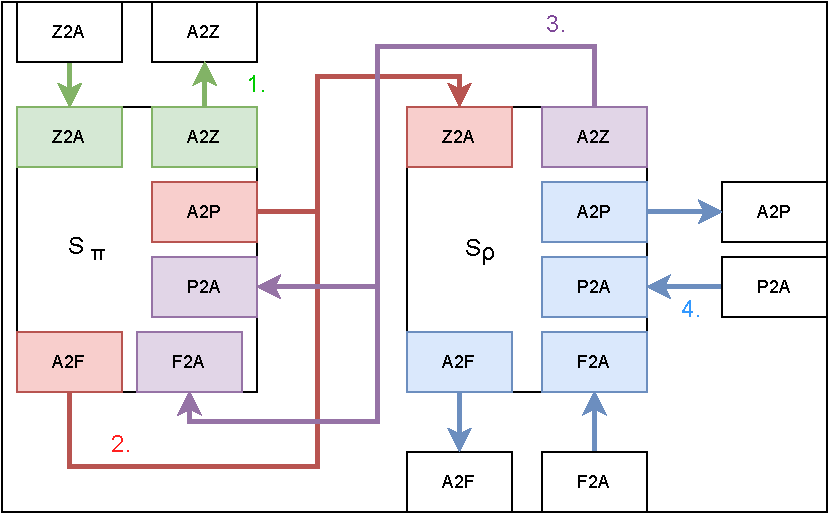
\includegraphics[scale=0.62]{figures/simcomp.pdf}
\caption{The composed simulators for $\F_1 \xrightarrow{\rho \circ \pi} \F_3$. The real world consists of $(\rho \circ \pi, \F_1)$. Inputs from \Z are for $\F_1$ and dummy parties interacting with $\F_1$, which \SIM{\pi} is equipped to handle. Outputs from \SIM{\pi} are for $\F_2$ and dummy parties of $\F_2$ which \SIM{\rho} is equipped to handle. FInally, outputs from \SIM{\rho} are for $\F_3$ and dummy parties of $\F_3$, which is just the ideal world in Theorem~\ref{thm:composition}.}
\label{fig:simcomp}
\end{figure}

%\begin{lstlisting}[basicstyle=\small\BeraMonottFamily, mathescape, frame=single]
%m = recv $\$$p2a ;
%case m (
%  P2A(pid, msg) =>
%   	case msg (
%      Committed =>
%        h = sample r k ;
%        send $\$$z2a P2A2Z(pid, (h)) ;
%      Open(b) =>
%	    x = sample r k ;
%        send $\$$z2a P2A2Z(pid, SMsg(b, x)) ;
%\end{lstlisting}

%When the committer is corrupt, the simulator has to do more work. 
%The key point that makes commitment in the RO model realizable is that \Z acquires commitment to give to the corrupt committer from \Fro through \A. 
%In th ideal world, the simulator recrods all the (key,value) pairs generated by its simulation of \Fro and therefore can always determine the bit \Z is committed to.
%When \Z queries \Sim with \inline{Z2A2F(SHash(b + x))} it stores the value and generates a hash value for it and returns it to \Z. 
%When instructed to give input to the corrupt party the simulator, \Sim gives input \inline{A2P(1, Commit(b))} where $b$ is the bit whos hash was requested.
%
%There is a unique edge case where \Z give some random bit sequence to \S as the commitment which wasn't generated by the random oracle. 
%In this case \S chooses a bit at random annd passes \inline{A2P(1, Commit(b))} to the protocol wrapper where $b$ is randomly selected.
%When prompted to open the commitment, \S does nothing as the real world receiver would fail to confirm whether the commitment corresponds to the bit $b$.




%\subsection{Ideal World}
%We described the functionality \Fcom in detail in Section~\ref{sec:execuc} as well as the functionality wrapper construction around it.
%We now describe how we implement ideal world (dummy) parties.

%We first describe at a high-level, the conversion happening within the functionality wrapper for \Fcom with the \inline{commit} message sent by the sender.
%When the wrapper receives the \inline{commit} message, the functionality wrapper executes the following:
%\begin{lstlisting}[basicstyle=\small\BeraMonottFamily, frame=single, mathescape]
%$\tg{(* l1 : list[pid \textasciicircum sender] *)}$
%case $\$$p2f (
%  yes => 
%    pid = recv $\$$p2f ; msg = recv $\$$p2f ;
%    case msg (
%      Commit(b) => 

%        $\$$ch_ = get_channel_by_pid pid $\$$l1 $\$$l2 ... ;
%        $\$$ch_.commit ;
%        send $\$$ch_ b ;
%        $\$$l2' <- append $\$$ch_ $\$$l2 ;
%\end{lstlisting}
%The wrapper also spawns a process to read from each of \Fcom's outgoing channels, case analyze on their value and send out the corresponding functional message to the protocol wrapper.

%The \msf{execUC} function in Figure~\ref{lst:execuc} accepts some number of type parameter which it spawns the main channels of the protocol with. 
%Most important out of these channels is the types governing communication between \Z and \A and between \Z and the protocol wrapper.
%If the types for these channel in both worlds aren't the same, even the import token expected, then it is trivial for an environment to distinguish the two worlds.
%It suffices to specify the import type parameters (\inline{p2f}, \inline{f2p}, \inline{z2p}, etc.) to \inline{execUC}.
%\paragraph{The Ideal World Execution}
%We summarize the message types in use by describing the type parameters to the ideal world execution.
%For the ideal, \inline{execUC} is invoked as follows (refer to the \inline{execUC} definition in Figure~\ref{lst:execuc} for what each of the parameters refers to):
%\begin{lstlisting}[basicstyle=\small\BeraMonottFamily, frame=single, mathescape]
%$\Type$ z2amsg[a][b] = Z2A2P of pid ^ a 
%                     | Z2A2F of b ;
%$\tg{(* ideal world *)}$
%execUC[K1,K2][comf2p][comp2f][comp2f][comf2p]
%  [comf2p][comp2f][comf2a][coma2f][rof2a][roa2f]
%  [rof2p][rop2f]
%\end{lstlisting}
%%$\tg{(* real world *)}$
%%execUC[K1,K2][comf2p][comp2f][rop2f][rof2p]
%%  [rof2p][rop2f][comf2a][coma2f][rof2a][roa2f]
%%  [rof2p][rop2f]
%Notice that the message types over \inline{p2z} and over \inline{p2f} are the same, because the ideal world parties are dummy parties which simply forward the messages to \Fcom.
%The type parameters for the adversary in the ideal world, though, still take the form of the types of \Fro.
%This is because the inputs \Z gives to both worlds (the dummy adversary in the real world) is intended for \Fro when communicating with the functionality through the adverasary or through corrupt parties 
%
%The party inputs from \inline{a2p} in the ideal world are intended for \Fcom, not \Fro, so they are of the same type \inline{comp2f}.
%Similarly, output from corrupt parties to the adversary in the ideal world is the same as output from \Fcom, and, therefore the message type is the same as \inline{comf2p}.
%The messages type parameters are wrapped in channel-specific types as well.
%For example, the channel \inline{z2a} is typed as follows:
%\begin{lstlisting}[basicstyle=\small\BeraMonottFamily, frame=single, mathescape]
%type z2amsg[a][b] = Z2A2P of pid ^ a
%                      | Z2A2F of b ;
%#z_to_a: comm[z2amsg[a2p][a2f]]
%$\tg{(* a2p=rop2f, a2f=roa2f in execUC above*)}$
%\end{lstlisting}
%
%\paragraph{Ideal Protocol}
%The ideal world protocl is a dummy party which forwards all messages to the functionality. 
%The message content from \inline{z2p} and \inline{p2f} is the same in the ideal world, but it is wrapped in different parameteric typed when it is sent from the \inline{z} or \inline{p}.
%As shown below the messages themselves are the same (\inline{comp2f} but typed differently (\inline{z2pmsg} vs \inline{p2fmsg}):
%\begin{lstlisting}[basicstyle=\small\BeraMonottFamily, frame=single, mathescape]
%$\Type$ z2pmsg[a] = Z2P of pid ^ a ;
%$\Type$ p2fmsg[a] = P2F of pid ^ a ;
%#z_to_p: comm[z2pmsg[comp2f]] ;
%#p_to_f: comm[p2fmsg[comp2f]] ;
%\end{lstlisting}
%The protocol wrapper only needs to forward the message unaltered but using a different type construtor. 

%The ideal functionality \Fcom is the same one introduced in Figure~\ref{fig:fcom} in Section~\ref{sec:nomosuc}. 
%In FIgure~\ref{lst:fcom} we present the Nomos definition of the same functionality and provide the channel types in FIgure~\ref{fig:fcomtypes}.
%We elide some of the clutter of acquiring and releasing shared channels in the form of: \texttt{\$p2f $\leftarrow$ acquire \#p\_to\_f} for clarity. 
%Wherever a linear channel like \texttt{\$p2f} is used it is in fact an acquired shared channel \texttt{\#p\_to\_f}.
%
%The key difference to note between \Fcom and its Nomos version is that the functionality is split up into two processes rather than compressed into one.
%This design decision is required because of how Nomos cycles between processes in a round-robin fashion and the communicator design.
%Therefore, processes must recurse when there is no message to be read and move to the next processes after the first expected message is received--in this case the \msf{P2FCommit(b)} message.
%
%
%\begin{figure}
%\centering
%\msf{type} \msf{Ip2f} = \msf{P2FCommit} of \msf{Bit} | \msf{P2FOpen}
%
%\msf{type} \msf{If2p} = \msf{F2PCommit} | \msf{F2POpen} of \msf{Bit}
%
%\msf{type} \msf{Ip2f} = \msf{SCommit} of Bit | \msf{SOpen}
%
%\msf{type} \msf{If2p} = \msf{RCommit} | \msf{ROpen} of Bit
%
%\msf{type} \msf{Rp2f} = \msf{SHash} of \msf{Int} | \msf{Send} of \msf{pid} \textasciicircum \msf{pid} \textasciicircum \msf{Int}
%
%\msf{type} \msf{Rf2p} = \msf{Pre} of \msf{Int} | \msf{RHash} of \msf{Int} | \msf{MSG} of \msf{pid} \textasciicircum \msf{pid} \textasciicircum \msf{Int}
%
%\caption{Types for the channels in the ideal world for \Fcom. Notice that Ip2f and If2p is the type of the channels \msf{z2p} and \msf{p2z} as they much match for both worlds and the ideal world parties simply forward messages to the functionality. The \msf{p2f} and \msf{f2p} channels are specific to the real and ideal world as the functionalities are not the same. Hence the real-world \msf{p2f} is typed with \msf{Rp2f} for the random oracle and the ideal world \msf{p2f} is typed with \msf{Ip2f} for \Fcom.}
%\label{fig:fcomtypes}
%\end{figure}
%
%\begin{figure*}
%\begin{lstlisting}[basicstyle=\small\BeraMonottFamily]
%proc F_code:
%  (s: sid), (k: Int), (rng: [Bit]), (clist: list[Int]),
%  (#p_to_f: comm[pid ^ Ip2f]{Ip2fn}), (#f_to_p: comm[pid ^ If2p]{If2pn}),
%  (#a_to_f: comm[Ia2f]{Ia2fn}), (#f_to_a: comm[If2a]{If2an})  |- ($ch: FtOE) =
%{
%  case $p2f (
%    yes =>	
%      pid, msg = recv $p2f ;
%      get $pwf {Ip2fn} ;
%      case msg (
%        P2FCommit(b) =>	
%          if pid == 1
%          then
%            send F2PCommit $f2p ;
%            pay {If2pn} $f2p ;
%            $ch <- F_com_open s k rng clist #p_to_f #f_to_p b ;
%          end
%      )
%   | no =>  
%       $ch <- F_code s k rng clist #p_to_f #f_to_p ;
%  )
%}
%
%proc F_code_open:
%{
%  case $p2f (
%    yes =>	
%      pid, msg = recv $p2f ;
%      get $p2f {0} ;
%      case msg (
%        P2FOpen =>	
%          if pid == 1
%          then
%            send F2POpen(b) $f2p ;
%            pay {0} $f2p ;
%            $ch <- 1 ;
%          end
%      )
%   | no =>
%       $ch <- F_code_open s k rng clist #p_to_f #f_to_p b ;
%  )
%}
%\end{lstlisting}
%\end{figure*}
%
%The real world protocol for commitment follows a simple communication patter:
%\begin{enumerate}
%\item On input bit $(\msf{P2FCommit}\ b)$ from the environment, the committer queries the random oracle with the message $(\msf{SHash}\ b | r)$ where $r \xleftarrow{\$} \{0,1\}^k$.
%The returned ``hash value'' is sent to the receiver as the commitment.
%\item On input \msf{P2FOpen} from \Z, the committer sends $(\msf{Send}\ p_L\ b\ r)$ to the receiver.
%\item The receiver checks that the commitment is correct be querying \Fro in the same way and asserting that the has returned $(\msf{RHash}\ h)$ is the same as the one sent by $p_C$.
%\item \todo{the type of Rf2p is kind of wrong so need to correct it}
%\end{enumerate}
%
%We provide only a simulator for the dummy adversary as that guarantees a simulator for all adversaries required our emulation definition.
%The simulator for commitment is relatively simple so we only provide a high-level description here and leave the full simulator code to the appendix.
%The simulator internally simulats the random oracle by maintaining a table of key-value pairs that it can control entirely.
%If the committer is corrupt:
%\begin{enumerate}
%\item The simulator can not determine the bit \Z wants to commit to so selects a random bit when activatd by the environment and gives it as input to the corrupted committer.
%\item When it's asked to open the commitment it simply forwards the request to the corrupt committer and stops.
%\end{enumerate}
%If the receiver is corrupt:
%\begin{enumerate}
%\item When activated by the receiver with (\msf{F2PCommit}), the simulator generates some random string $h$ to represent the commitment, stores it, and sends ($\msf{P2A}\ \msf{MSG}(p_C, p_R, h)$) to \Z.
%\item When it receives ($\msf{F2POpen}\ b$) from the receiver, it returns $(\msf{P2A}\ \msf{MSG}(p_C, p_R, b, r)$ to \Z where $r$ is a randomly generated sequence keeping the pair $(b | r, h)$ as the corresponding entry in the table.
%\item When activated by \Z to check the commitment, \Sim simply returns the commitment hash or creates a new one.
%\end{enumerate}
%
%\paragraph{Simulator Well-Matched}
%It is immediately obvious that the constructed simulator is well-typed if the dummy adversary is well-typed with the given type parameters.
%The simulator receives 1 import token per activation from \Z which suffices to simulated \Fro internally. 
%Subsequently, \Sim keeps all of the import it receives, and, therefore when one of the partiesis corrupt a simple bounding polynomial can be given as:
%\[
%	T_{\Dummysim}(n) = T_{\Fro}(n) + O(1)
%\]
%where $T_{\Fro}$ is a satisfying polynomial for \Fro. The additional constant factor simply accounts for sending messages to the corrupt parties.
%Therefore,
%\begin{gather}
%	\forall \Z, \langle \Z \leftrightarrow \DA \rangle \Rightarrow \langle \Z \leftrightarrow \Dummysim \rangle
%\end{gather}
%
%
%\begin{figure*}
%\begin{lstlisting}[basicstyle=\BeraMonottFamily]
%(* Z2P interface *)
%type Ip2f = P2FCommit of Bit | P2FOpen ;
%type If2p = F2PCommit | F2POpen of Bit ;
%
%(* Ideal World *)
%type Ip2f = SCommit of Bit | SOpen ;
%type If2p = RCommit | ROpen of Bit ;
%
%type Ia2f = 0 ;
%type If2a = 0 ;
%
%type Ia2p = Ip2f ;	(* crupt input is same as z2p *)
%type Ip2a = If2p ;
%
%(* Real World *)
%type Rp2f = SHash of Int | Send of pid ^ pid ^ Int ;
%type Rf2p = Pre of Int | RHash of Int | MSG of pid ^ pid ^ Int ;
%
%type Ra2f = A2Hash of Int ;
%type Rf2a = Hash2A of Int ;
%
%type Ra2p = Rp2f ;
%type Rp2a = Rf2p ;
%
%(* the import here is given as those for the dummy adversary in the real world *)
%p2zn <- 0 ; z2pn <- 1 ;
%a2zn <- 0 ; z2an <- 1 ; 
%
%Rf2pn <- 0 ; Rp2fn <- 1 ;
%Rp2an <- 0 ; Ra2pn <- 1 ;
%Rf2an <- 0 ; Ra2fn <- 1 ;
%
%If2pn <- 0 ; Ip2fn <- 0 ;
%Ip2an <- 0 ; Ia2pn <- 0 ;
%I
%
%(* channels *)
%#z_to_p <- comm[pid ^ Ip2f]
%#p_to_z <- comm[pid ^ If2p]
%#z_to_a <- comm[ z2d[Ra2p][Ra2f] ] ;
%#z_to_z <- comm[ d2z[Rp2a][Rf2a] ] ;
%
%
%(* Real World exec PI *)
%execUC[Ip2f][If2p][Rp2f][Rf2p][Rp2a][Ra2p][Rf2a][Ra2f][a2z][z2a]
%	  {p2zn}{z2pn}{f2pn}{p2fn}{p2an}{a2pn}{f2an}{a2fn}{a2zn}{z2an}
%
%(* Ideal world exec PHI *)
%execUC[If2p][Ip2f][Ip2f][If2p][Ip2a][Ia2p][If2a][Ia2f][a2z][z2a]
%	  {p2zn}{z2pn}
%
%
%
%
%
%
%\end{lstlisting}
%\end{figure*}


The type system in NomosUC helps to identify when the amount of potential that a functionality requires isn't satisfied by the bounding polynomia given.
We illustrate this point using the $\F_{\msf{map}}$. 
The functionality maintains a list that parties can append to the end of or read from.


%\caption{The $\mathcal{F}_{\msf{comm}}$ commitment ideal functionality in Nomos. The types for the sender and receiver channel define what inputs they can give to the functionality and what messsages are sent from the functionality back to the receiver.}
%\label{fig:nomos:commitment}
%\end{figure*}



\section{Import in NomosUC} \label{sec:motivate}
In this section we discuss how import is encoded into session types, how processes in NomosUC use import, motivate our adaptation of import into \emph{import session types} (IST), and the relevant type rules for making judgements on polynomial time.
IST allows processes to send import to each other algonside messages, like import between ITMs, but concretizes the accounting of actual computation steps through a resource called \emph{potential}~\cite{das2018work,dasnomos}.
Recall that an ITM that possesses $n'$ net import (= import received - import sent) can do at most $T(n')$ computation for some polynomial $T$.
In NomosUC, we say that a process with this import posseses at most $T(n')$ potential.
Runtime in IST is checked against a user-defined polynomial that is provided as a parameter at comple-time.

Unlike import, potential is never exchanged between processes, but is generated by ``consuming'' import.
Generating potential creates a runtime budget for the process, affects the amount ot import it has remaining, and makes explicit how much import has been ``consumed'' by the work already done.
For example, if a process with potential $T(n')$ generates $X < T(n')$ potential, then it can only send $k$ import to another process if $X \leq T(n'-k)$.
%Generated potential creates a runtime budget for the calling process and affects the amount of import it has remaining and makes explicit how much import is ``consumed'' by the process: if a process $P$ with $n'$ tokens generates $X$ potential and performs work $X < T(n')$ it can only send $k$ import if $X \leq T(n'-k)$.
Concretizing execution through potential as a resource allows us to make this judgement in the type system. 


\paragraph{Why another resource?} 
%Why is it necessary to add another resource on top of import rather than directly account of runtime through import?
We first address the question of why another resource is needed to bound the execution of indivual processes rather than treating import as the direct accounting value.
%In general, an arbitrary mechanism for bounding runtime can be realized by a linear resource (like in Das et al.~\cite{das2018work}), but absracting runtime through a polynomial in import is critical and requires a separate resource to track work performed.
This design is motivated, and hinted at, by Canetti~\cite{canettiUC} in the formulation of UC and the import mechanism, and we largely defer to the framework to motivate and explain it.
%In the general case of bounding runtime, a single linear resource is sufficient to control the runtime of processes (like the work by Das et al.~\cite{rast}), however, in UC we are concerned with capturing a realistic computation model and doing so leaks information that otherwise shouldn't be known. 
At a high level, the primary reason is that using import as the the unit of computation allows an ITM to precisely control the runtime of another that it gives import to.
Fundamentally, this would require ITMs to know before-hand the amount of computation another ITM will do in order to give it sufficient import.
Furthermore, this allows the environment, which gives messages and import to both the real and ideal world, to limit the computational power of the two worlds and gives it extra information with which to distinguish between them.
The ideal world functionality and the real world protocol will certainly perform different amounts work as they are different programs, and, therefore, terminate at different times~\footnote{A protocol that realizes \Fcom will do much more computation and message-passing between the two parties whereas \Fcom terminates just after accepting two inputs and storing the committed bit}. 
If \Z can force one world to terminate and the other to not, it can easily distinguish between them, and does so with information that isn't legitimately known to it in any reaslistic model.
\footnote{The specific example given by Canetti~\cite{canettiUC}: ``For instance, the initial ITI $I$ can start in a rejecting state, and then pass control to another ITI $M$. If $I$ ever gets activated again, it moves to an accepting state. Whether $I$ is activated again depends on the running time of $M$. If it exceeds the computation given to it (known by $I$) then $I$ accepts depending on information that should not be ``legitimately known'' to $I$.}.


%The database functionality performs potentially quadratic work, in total, in the number of items stored (or, equivalently, in the number of activations): a sequence of $n$ inserts and queries results in $O(n^2)$ work iterating over $\ell$.
%In this section we introduce how processes like \Fdb receive and use import, motivate our design for adding import to NomosUC, and the relevant typing rules for making judgements on polynomial time.
%Specifically, we adapt import into session types and create \emph{import session types} (IST).
%IST allows processes to send each other import over channels and accounts for the number of computation steps a process can take through a resource called \emph{potential}~\cite{das2018work,dasnomos}.
%Recall that an ITM that possesses $n'$ net import (= import received - import sent) can do at most $T(n')$ computation for some polynomial $T$.
%In NomosUC, we say that such an ITM has at most $T(n')$ potential.
%Runtime in IST is checked against a concrete polynomial given as a parameter at compile time. 
%We account for the actual work performed by a process with \emph{potential} where every step costs 1 unit of potential.

%\paragraph{Why another resource?} 
%%Why is it necessary to add another resource on top of import rather than directly account of runtime through import?
%In general, an arbitrary mechanism for bounding runtime can be realized by a linear resource (like in Das et al.~\cite{das2018work}), but absracting runtime through a polynomial in import is critical and requires a separate resource to track work performed.
%This design is motivated by Canetti~\cite{canettiUC}.
%%In the general case of bounding runtime, a single linear resource is sufficient to control the runtime of processes (like the work by Das et al.~\cite{rast}), however, in UC we are concerned with capturing a realistic computation model and doing so leaks information that otherwise shouldn't be known. 
%At a high-level, using import as the the unit of computation allows an ITM to precisely control the runtime of an ITM it gives import to, giving it information about the other's state that, realistically, it shouldn't know.
%For example, imagine a real world and an ideal world where the environment uses import to control exactly the number of steps each world is can take.
%The differing ITMs will perform different work and terminate at different times, and \Z can use this information to artificially distinguish between them.
%\footnote{The specific example given by Canetti~\cite{canettiUC}: ``For instance, the initial ITI $I$ can start in a rejecting state, and then pass control to another ITI $M$. If $I$ ever gets activated again, it moves to an accepting state. Whether $I$ is activated again depends on the running time of $M$. If it exceeds the computation given to it (known by $I$) then $I$ accepts depending on information that should not be ``legitimately known'' to $I$.}.


\subsection{Giving Runtime To Processes}
We introduce two new type constructors to define the import sent with messages using IST: $\getpot$ and $\paypot$.
They are highlighted in red in the session types for \Fcom and \Fro above.
Canonically, the internal choice operator $\ichoice$ is paired with $\getpot$ and the external choice $\echoice$ with $\paypot$.

In the case of \Fcom, sender must always send two import when sending label $\mb{commit}$ and none when sending $\mb{open}$.
Similarly, \Fcom sends one import to the receiver when sending label $\mb{rcommit}$ and none when sending $\mb{ropen}$.
In UC, the adversary never receives any import from a functionality or protocol parties. 
In the case of \Fro, every party must give import on a query for a hash value and never gets any in return.

The random oracle, over the course of an execution needs to store a list of all the values queries and may be activated a polynomial number of times.
Hence, we require that it always possess some import to perform such a computation. No import at all would allow it to perform constant $T(0)$ work across all activations.
The ideal commitment, on the other hand, is single-shot and does a constant amount of work. 
A natural question is why it requires any import, let alone two, and why does it give import to the receiver?
Recall that a prerequisite for emulation is that the session types in the real and ideal world match exactly. 
Setting \m{sender} and \m{receiver} this way ensures that a protocol that realizes \Fcom can perform some non-trivial computation.
In general, defining an ideal functionality with a specific amount import can be restrictive as to which protocols can realize it so it makes sense to sometimes define them as parameteric in the amount of import trasnferred.

\paragraph{Exchanging Import in NomosUC}
The new type operators for import in IST are paired with two new operators in process code: \ipay and \iget.
In sender code for \protcom in Figure~\ref{fig:fcom}, we see the sender explicitly gets two import from \zp that the session type requires (line 7).
Similarly, \Fro requires one import to be paid to perform a hash (line 9).
The type system that we describe later on requires that at any point in execution a process can never send import it doesn't possess, and that it's execution is always bounded by the net import it possesses.
This excludes situations where two processes infinitely send the same import token back to each other.


%\subsection{Giving Import to \Fdb}
%Quadratic work over $n$ insertions and accesses to \Fdb, necessitates import linear in $n$.
%Therefore, we add an import requirement to the session types between \Fdb and the protocol parties (and \A).
%
%%We introduce \emph{import session types (IST)} to express and exchange import between processes. 
%%Unlike resource-aware session types, resource sent with import session types implies computation polynomial in the amount sent rather than linear. 
%We introduce two new type constructors:  $\getpot$ and $\paypot$.
%The \Fdb session type now becomes:
%\begin{tabbing}
%    $\mi{type} \; \m{db[k][v]} = \ichoice{$\=$\textcolor{red}{\paypot{1}}$\=$ \; \mb{store}:\m{PID} \arrow \m{k} \arrow$ \\
%    \>\>$\echoice{ \mb{OK}: \m{PID} \arrow \m{db[k][v]}},$ \\
%    \>$\textcolor{red}{\paypot{1}}$\=$ \; \mb{get}: \m{PID} \arrow \m{k} \arrow$ \\
%    \>\>$\echoice{$\=$\mb{yes}: \m{v} \arrow \m{db[k][v]},$ \\
%    \>\>\>$\mb{no}: \m{db[k][v]}}}$
%\end{tabbing}
%The calling party sends import using the $\paypot$ operator and \Fdb sends import using the $\getpot$ operator.
%In this case, the type enforces that 1 import token is sent when a party takes the $\ichoice$ and calls \Fdb, and \Fdb never sends any import back.
%\footnote{Rather than explicitly place a $\textcolor{red}{\getpot{0}}$ we omit the operator altogether.}
%This session type ensures \Fdb possesses $n$ import after $n$ activations. 

%In NomosUC process code, we introduce new operations to let processes exchange the import specified by the session type and use potential to account for the work done.
%The same \Fdb process code from Section~\ref{sec:example} is augmented with the commands \inline{$\nget$} and \inline{$\npay$} for sending/receiving import. 
%Below we show the case of \inline{store} in \Fdb and the corresponding party paying the import (lines 6 and 4, in \red{red}).
%\begin{lstlisting}[basicstyle=\scriptsize\BeraMonottFamily, frame=single, mathescape, numbers=left, xleftmargin=2em, xrightmargin=2em,firstnumber=3]
%$\tg{...}$
%$\ncase$ $\$$p2f (
%  store => pid,(k',v') = $\nrecv$ $\$$p2f
%    $\tr{get {1} \$p2f}$
%    $\ngenpot$(length l + 2)
%    $\ntick$(1)
%    $\$$tb' <- pappend[(k,v)] <- $\$$tb k' v' ;
%    $\ntick$(1)
%    $\$$p2f.Ok; $\nsend$ $\$$p2f pid ;
%    $\$$c $\leftarrow$ Fdb[k][v] <- $\tg{(* args *)}$ $\$$tb'
%$\tg{...}$
%\end{lstlisting}
%$\nproc$ Fdb[k][v]: ($\$$p2f: db[k][v]), ($\$$f2p: 1), 
%  ($\$$a2f: adv[k][v]), ($\$$f2a: 1), (l: [(k,v)]) |- ($\$$c: 1) =
%{

%    retrieve => pid,k' = $\nrecv$ $\$$p2f ;
%      $\tr{get {1} \$p2f}$
%      b $\leftarrow$ exist $\leftarrow$ $\$$tb k' ;
%      $\nif$ b $\nthen$
%        v' $\leftarrow$ get $\$$tb k' ;
%        $\$$p2f.yes; $\nsend$ $\$$p2f pid; $\nsend$ $\$$p2f v';
%      $\nelse$
%        $\$$p2f.no; $\nsend$ $\$$p2f pid ;
%      $\$$c $\leftarrow$ Fdb[k][v $\leftarrow$ $\tg{(* args *)}$ 
%\begin{lstlisting}[basicstyle=\scriptsize\BeraMonottFamily, frame=single, mathescape, numbers=left, xleftmargin=2em, xrightmargin=2em,firstnumber=4]
%$\$$p2f.store ; $\tr{pay {1} \$p2f}$
%$\nsend$ $\$$p2f pid ; 
%$\nsend$ $\$$p2f someK ; $\nsend$ $\$$p2f someV ;
%$\ncase$ $\$$p2f ( Ok => 1 )
%\end{lstlisting}
%$\nproc$ somparty[k][v]: (pid: PID), ($\$$p2f: db[k][v]), 
%  ($\$$f2p: 1)  |- ($\$$c: 1) =
%{
%}

%\subsection{Potential Mechanism}
%Import in UC allows for polynomial runtime, and, in a sense, import is \emph{consumed} when a computation is performed. 
%The UC security definition only cares that there is \emph{some} polynomial to bound an ITM's runtime.
%In NomosUC, we are explicit about the polynomial used, and type-checking a collection of processes relies on a concrete polynomial that runtime is checked agains.
%In order to actually account for runtime, another concrete value is needed: \emph{potential}.
%
%The potential mechanism directly determines how much import a process has actually consumed by measuring how much comutation it does and is still able to do.
%Specifically, we want to ensure the following situation is caught by NomosUC.
%Two processes $A$ and $B$ shouldn't be able to send 1 import back and forth and \emph{both} perform polynomial from that 1 token.
%
%For example, when a process $A$ sends import to another process, the type system must ensure
%that the computation already performed by $A$ is still polynomially bounded by the import remaining after sending import.
%In other words, two processes $A$ and $B$ shouldn't be able to send 1 import back and forth and perform polynomial from that 1 token.
%$A$ performing a polynomial computation with the single import and sending it to $B$ should fail to type check. 
%Potential is related to import by the following statement: if a process
%possesses $n`$ net import then it has potential of $T(n')$, and it can not take more than $T(n')$ computational steps.
%Potential is never exchanged between processes and is checked in relation to the net import a process has. If a process performs 
%$X < T(n)$ steps and sends an import to another process such that $X > T(n-1)$, NomosUC fails to type-check the process (we leave all typing rules to the end of the section).

\paragraph{Potential}
NomosUC processes must be explicity about how much potential they use through two new keywords: \inline{$\ngenpot$} and \inline{$\ntick$}.
A UC proof on paper can theoretically reason about the execution of a ITM, but we require a concrete accounting mechanism for doing the same for NomosUC processes. 
The type system tracks, for every process, the cumulative amount of potential generated by the process, $q$, and the current remaining potential, $q'$. We elaborate on the details of the type system in a later section.
To perform $r$ work, a NomosUC process must first $r$ potential with \inline{$\ngenpot$}(r) resulting in $q+r$ and $q'+r$ potential (line 7).
The then process accounts for taking $x$ steps by calling \inline{$\ntick$(x)} resulting in remaining potential $q'-x$ (lines 8, 10)
We exclude the calls to \igp and \itick in Figure~\ref{fig:fcom} to save space, but, in general, instead of manually inserting a \itick everywhere, NomosUC can be instrumented to insert a \itick before every operation that it performs.
The typing rules at the end of the section use $q$ and $q'$ to judge \emph{valid} NomosUC processes.
%The function call to \inline{pappend} performs \itick operations, but the calling process generates the potential.
%Therefore, conservatively, \Fdb generates enough potential to expend unit cost for accessing each item in the list (line 4).
%In this code section, we rely on \inline{pappend} to execute \inline{$\ntick$} operations of it own, and \Fdb and deducts potential before performing a message send back to the party (line 7).
%\begin{lstlisting}[basicstyle=\scriptsize\BeraMonottFamily, frame=single, mathescape, numbers=left, xleftmargin=2em, xrightmargin=2em]
%$\tg{...}$
%$\ncase$ $\$$p2f (
%  store => pid,(k',v') = $\nrecv$ $\$$p2f
%    $\tr{get {1} \$p2f}$
%    $\ngenpot$(length l)
%    $\$$tb' <- pappend[(k,v)] <- $\$$tb k' v' ;
%    $\ntick$(1)
%    $\$$p2f.Ok; $\nsend$ $\$$p2f pid ;
%    $\$$c $\leftarrow$ Fdb[k][v] <- $\tg{(* args *)}$ $\$$tb'
%$\tg{...}$
%\end{lstlisting}
%Additionaly, abstracting import into a sub-resource called potential makes the UC framework all the more expressive.
%If import was used to count and bound computation directly, rather than through a polynomial, the \Fdb example becomes untennable. 
%A party querying \Fdb has to know how long the list is so it sends enough import to iterate over it, and it doesn't know how many items other parties may have added.
%This leads to a bizarre setting where parties must attempt to learn information about the list size or keep trying higher increments of import to complete a query.
%Constraining runtime in this way makes the framework unnecessarily cumbersome.

%Imagine the database session type specified 1 import token is exchanged in both directions: 1 token from parties when querying and 1 token back from \Fdb with the result. 
%Without a concrete resource to track the actual com
%For example, without the potential mechanism the following processes set would type check but obviously violates the rules of import. 
%
%\begin{tabbing}
%   $\mi{type} \; \m{atob} = \ichoice{\textcolor{red}{\paypot{1}} \; \mb{give}: \echoice{\textcolor{red}{\getpot{1}} \; \mb{receive}: \m{atob}}}$
%\end{tabbing}
%
%\begin{lstlisting}[basicstyle=\footnotesize\BeraMonottFamily, mathescape, frame=single]
%$\nproc$ A : (bigNumr: Int), ($\$$a2b: atob) |- ($\$$ch: 1) = {
%  $\text{\color{Red}{genPot k}}$
%  let bigNum = bigNum * 2 ;
%  $\$$a2b.give; $\npay$ {1} $\$$a2b ;
%  $\ncase$ $\$$a2b ( receive => $\nget$ {1} $\$$a2v )
%  $\$$ch <- A bigNum $\$$a2b ;
%}
%
%$\nproc$ B : (bigNum: Int), ($\$$a2b: atob) |- ($\$$ch: 1) = {
%  $\ncase$ $\$$a2b (
%    give => $\nget$ {1} $\$$a2b ;
%      $\text{\color{Red}{genPot k}}$
%      $\nlet$ bigNum = bigNum * 2 ;
%      $\$$a2b.receive ; $\npay$ {1} $\$$a2b ;
%      $\$$ch <- B <- bigNum $\$$a2b ;
%  )
%}
%\end{lstlisting}
%
%Without additional rules for accounting for potential (lines 2 and 12), and \emph{consuming} import, the above system would violate the basic import mechanism as defined by UC.

%Furthermore, abstracting potential from import has the added benefit of a more expressive framework.
%Take the database ideal functionality below as an example. 
%When a party performs a read, it doesn't know the size of the list before-hand. 
%Using only import as the accounting for computation, the protocol party would always have to give a precise amount of import to ensure the whole list can be read. 
%With potential, a single unit of import is enough for the functionality to determine how much polynomial computation (in this case, linear) needs to be done.  
%
%\begin{tabbing}
%   $\mi{type} \; \m{db[k][v]} = \ichoice{$\=$\textcolor{red}{\paypot{1}}$\=$ \; \mb{store}:\m{PID} \arrow \m{k} \arrow$ \\
%   \>\>$\echoice{ \mb{OK}: \m{PID} \arrow \m{db[k][v]}},$ \\
%   \>$\textcolor{red}{\paypot{1}}$\=$ \; \mb{get}: \m{PID} \arrow \m{k} \arrow$ \\
%   \>\>$\echoice{$\=$\mb{yes}: \m{v} \arrow \m{db[k][v]},$ \\
%   \>\>\>$\mb{no}: \m{db[k][v]}}}$
%\end{tabbing}
%
%\todo{fdatabase is nontrivial, how much of it to include? maybe only where it iterates over the list and generates n potential to do it}
%\begin{bbox}[title={Functionality $\F_{\msf{db}}$}]
%
%Initialize list $l := []$
%
%\OnInput \inmsg{add}{$x$} form $P_i$:
%   \begin{ritemize}
%       \item Append $x$ to $\ell$
%       \item \Send $ok \rightarrow P_i$
%   \end{ritemize}
%
%\OnInput \inmsg{get}from $P_i$:
%   \begin{ritemize}
%       \item \Send $\ell \rightarrow P_i$
%   \end{ritemize}
%\end{bbox}

\subsection{Virtual Tokens}
Our realization of import so far adheres to the design specified by Canetti et al~\cite{canettiUC}.
We encounter a subtle problem realizing a common UC design pattern in NomosUC: ITMs sandboxing, or running internally, other ITMs.
Simulators, in particular, rely on this design pattern to emulate real-world protocols, rewind them, replay them, and override their randomness.
Allowing processes in NomosUC to do the same results in some issues with execution cost analysis.

\paragraph*{\textbf{A Constraint Unique to NomosUC}}
Simulators in UC often run other ITMs internally in a black-box manner. 
In NomosUC, doing the same with processes comes with the added constraints of satisfying the simulated process's session type.
Say a simulator \Sim that sandboxes \Fro internally. 
Ideally, we want that the computation done by \Fro counts towards the total work performed by \Sim rather that requiring import of its own like its session type requires.
Not doing so unecessarily restricts the kinds of simulators, and hence the kinds of proofs, that NomosUC can realize.
Without a way to give \Fro some ``fake'' import, we run into the constraint illustrated by the following simple example.

Imagine an adversary in the real world that accepts one unit of import and uses it to query \Fro.
The ideal world simulator is given the same single unit of import as the real world adversary, by definition, and if it must expend it to sandbox \Fro then it's left with no import to do anything else.
This issue is further exacerbated when you consider \Sim simulating the entire real-world execution. All of its import budget is used up running the same processes as the real world rather than the sandbox counting toward its total potential budget.
More generally, an ideal functionality in the real world, whose output depends on the amount of computation it's able to do, must perform exactly the same work when run by \Sim in order to produce the same output.
Therefore, we formulate a mechanism to create \emph{virtual tokens} to give to sandboxed processes that satisfy its import requirements while still only counting towards the total work done by \Sim.
Though a simple concept, realizing this in our typing rules is major contribution of this work.
\todo{Perhaps a good way to frame it is saying that the work \Sim could otherwise do with only 1 import (sandboxing + other stuff) it now needs 2 import to do. When \Sim needs to spend import in the ideal world as well, liek interacting with the ideal functuionality it is one short and show all definitioons hafve to change to accomodate this.}

%In the ITM model, in UC, a simulator, \Sim, sandboxing \Fdb has the ITM encoded on its own tape allowing it to arbitrarily manipulate its state and execute it as necessary.
%Therefore, the computaton that \Sim and the sandboxed \Fdb perform are counted as part of \emph{the same ITM}.
%In NomosUC, there is no notion of encoding \Fdb within \Sim without rewriting its code.
%Reusing \Fdb then means treating it as \emph{a separate process}, which is undesirable.
%%In NomosUC, running \Fdb in a similar way mean reimplementing the functionality as part of the process code of \Sim. Reusing the \Fdb process means \emph{it must be treated as a separate process} 
%%%barring reimplementing the functionality as part of the code of \S, \emph{it is must be treated as a separate process} 
%%with a session type \m{db[k][v]} which requires one import sent with every message.
%In the listing below, the simulator wants to run a copy of \Fdb and communicates with it over a channel \ic{fdb} (line 5). 
%\Z gives both the dummy adversary, \DA, and \Sim a message with 1 import (line 9) intended for \Fdb in the real world, and like \DA, \Sim calls \Fdb (line 12) with 1 unit of import due to its type \m{db[k][v]} (line 13).
%%\Sim relies on the existing process to emulate the outputs \Z would see in the real world communicating with the dummy adverasry and \Fdb.
%%On line 9, \Sim gets 1 unit of import from \Z, the same the \DA gets in the real-world, and on line 13 it's forced to give it up to make the call to \Fdb and not do any polynomial work itself.
%Without giving the import, \Sim would fail to type-check, but in doing so is forced to give up its own import.
%
%More generally, a functionality in the real world, whose output depends on the amount of computation it's able to do, must do exactly the same work when run by \Sim to produce the same output.
%In the real world the dummy adversary, \DA, receiving $X$ import from \Z gives all $X$ to \F and doesn't do any other work.
%In the ideal world, \Sim runs the the real-world internally, receives the same $X$ import as \DA, and must give \F all $X$ import to ensure the same output is produced. 
%It is therefore forced to give up it's entire runtime budget, just as \DA does, and therefore can't do any additional polynomial work of its own (line 18).

%Ultimately, simply running \Fdb as a separate process constrains the kinds of simulators (and so proofs) that can be realized, and if we want our cost analysis to treat \Fdb and \Sim as one and the same, a few important questions are raised:
%does \Sim lose import and \Fdb gains import? do they both share the same import because \Fdb is sandboxed? can we tell the type system to ignore import in IST in some cases?
%
%\begin{lstlisting}[basicstyle=\scriptsize\BeraMonottFamily, frame=single, mathescape, numbers=left, xleftmargin=2em, xrightmargin=2em]
%$\nproc$ sim_db[k][v] : 
%  $\tg{(* the usual params *)}$
%  ($\$$z2a: Z2A[a2p,a2f]), ($\$$a2z: A2Z[p2a,f2a]),
%  ($\$$p2a: a2p), ($\$$f2a: f2a),
%  ($\$$fdb: db[k][v]) $\tg{(*...*)}$ |- ($\$$c: 1) =
%{
% $\nmatch$ $\$$z2a,$\$$p2a,$\$$f2a (
%    Z2A2F,*,* =>
%      $\nget$ {1} $\$$z2a
%      msg = $\nrecv$ $\$$z2a
%      $\ncase$ msg (
%        Query(k) => $\$$db.query
%          $\npay$ {1} $\$$db
%          $\nsend$ $\$$db k
%          $\ncase$ $\$$db (
%            yes => v = $\nrecv$ $\$$db 
%            _ => ()
%          x $\leftarrow$ do_poly_work ;
%  $\tg{.....}$
%\end{lstlisting}
%        Store(k,v) => $\$$db.store
%          $\npay$ {1} $\$$db
%          $\nsend$ $\$$db k ; $\nsend$ $\$$db v
%          $\ncase$ $\$$db ( Ok => 
%            x $\leftarrow$ do_poly_work ;
%            $\$$c <- sim_db[k][v] $\tg{(* args *)}$ )
%}


%% | describe the a simulated \Fdb now without virtual tokens and showcase the issue
%% | and we need to be able to reuse process definitions rather than make special virtual one
The approach we take to support sandboxing is adding \emph{virtual import tokens} to NomosUC.
Rather than a single type of token, we allow NomosUC processes to create fake import tokens to give to sandboxed processes and tie the amount of virtual import created to the real import the process holds.
Tokens types are represented by a token hierarchy 
\vspace{-0.5em}
\begin{mathpar}
  \mi{token types\;}\;\K_0 \to \K_1 \to ... \to \K_m
  \vspace{-0.5em}
\end{mathpar}
Where $\K_0$ are real import tokens and $\K_{i>0}$ are all virtual.
The heirarchy is a global definition used by all processes, and the number of levels $m$ in the heirarchy is staticall defined, at compile-time, as the number of layers of sandbox within a sandbox.
The heirarchy is statically defined to prevent infinite type creation at runtime, and we are confident that the loss of expressivity is insignificant.
Process definitions change by accepted a type parameter, \inline{K} in the definition of \inline{protcom}, that specifies its token type that is set by the spawning process.
The main processes of the execution like the environment and adversary are spawned with type $K_0$ and sandbox processes with tokens $K_{i > 0}$. 
Sandboxing in this way also asserts that simulated processes can't communicate with processes outside of the sandbox due to a token type mismatch.

\plan{There used to be a code snippet here showing a process definition with the toke type paramter but it's useless we just point to the process definition of procom above}
%For example, the simulator above is now given the parameter $K_0$ (for real), and type $K_1$ as the virtual type to sandbox with:
%\begin{lstlisting}[basicstyle=\scriptsize\BeraMonottFamily, frame=single, mathescape, numbers=left, xleftmargin=2em, xrightmargin=2em]
%$\$$c $\leftarrow$ sim_db$\tr{[K0,K1]}$[k][v] $\tg{(* the usual params *)}$
%            $\tr{\^{}\^{}\^{}\^{}\^{}\^{}}$
%  ($\$$z2a: Z2A[a2p,a2f]), ($\$$a2z: A2Z[p2a,f2a]),
%  ($\$$p2a: a2p), ($\$$f2a: f2a) $\tg{...}$
%\end{lstlisting}
%The simulator, in turn, spawns an instance of \Fdb with a with  virtual token type, $K_1$ that \Fdb considers real tokens:
%\begin{lstlisting}[basicstyle=\scriptsize\BeraMonottFamily, frame=single, mathescape, numbers=left, xleftmargin=2em, xrightmargin=2em]
%$\$$fdb $\leftarrow$ Fdb$\tr{[K1]}$[k][v] $\leftarrow$ $\tg{...}$
%\end{lstlisting}

\paragraph{Creating Virtual Import}
A new NomosUC operation \inline{$\nwithdraw\ $ K0 K1 n} allows a process, using its real token type $K_0$, to create $n$ new tokens of type $K_1$, and we add a new parameter to $\npay$ and $\nget$ which specifies the token type being sent or received. 
A process $P$ can spawn a process $P'$ with a virtual type $K_1$ and can pay/receive virtual tokens to/from $P'$.
A process (below) that sandboxes $\Fro$ (above) spawns it with its virtual token type (line 1), create the virtual tokens it needs to send (line 2), and finally send the tokens specifying the type being sent by \inline{$\npay$} (line 3).
\begin{lstlisting}[basicstyle=\scriptsize\BeraMonottFamily, frame=single, mathescape, numbers=left, xleftmargin=2em, xrightmargin=2em]
$\$$ $\leftarrow$ Fro[K+1][(Int,Bit)] <- k sid rng $\$$p2f' $\$$f2p' $\$$a2f' $\$$f2a' 
$\nwithdraw$ K0 K1 1
$\$$p2f'.query ; pay $\textcolor{red}{K1}$ {1} $\$$p2f' 
$\nsend$ $\$$p2f' x
\end{lstlisting}
%When communicating with augmented \Fdb (above), \Sim (below) first creates the virtual tokens (line 5) and then sends them on the channel (line 6).
%Trying to give a type $K_i$ to a process whose real token type is some $K_{j \neq i}$ fails to type-check for obvious reasons.
%\begin{lstlisting}[basicstyle=\scriptsize\BeraMonottFamily, frame=single, mathescape, numbers=left, xleftmargin=2em, xrightmargin=2em]
%$\nget$ {1} $\$$z2a
%msg = $\nrecv$ $\$$z2a
%$\ncase$ msg (
%  Query(k) => 
%    $\nwithdraw$ K0 K1 1
%    $\$$db.query
%    $\npay$ $\tm{K1}$ {1} $\$$db
%    $\nsend$ $\$$db k
%    $\ncase$ $\$$db (
%      yes => v = $\nrecv$ $\$$db 
%      _ => )
%    x $\leftarrow$ do_poly_work ;
%\end{lstlisting}

\paragraph{Relating virtual tokens to real work.}
%Without relating virtual tokens to the amount of import that the sanboxing process has, we encounter an infinite runs problem where processes can continue to create virtual tokens and processes to perform super-polynomial work.
Intuitively, the number of virtual tokens created should be tied to the total runtime budget of the sandboxing process to prevent an infinite runs problem.
NomosUC constrains the number of virtual tokens created through a globally known polynomial \GlobalF defined at compile-time.
The type system requires that the virtual tokens of type $i+1$, $t_{i+1}$, created by a process $P_i$ are upper bounded by $\GlobalF(t_i, k)$ where $t_i$ is the number of tokens $P_i$ possesses of its real token type $K_i$ and $k$ is the security parameter.
%This ensures that over all virtual processes within a ``real'' process the amount of tokens is never super-polynomial in the number of real import.
The \inline{$\nwithdraw$} operator itself consume some potential, preventing a process from calling it indefinitely.
There are no potential types, like toke types, howeve the type system only compares the potential created/used to a polynomial in that process's token type. 
The typing rules described next clarify on how the type system determines whether a process satisfies import-based polynomial runtime.

%Our treatment of virtual tokens bounded by a polynomial in the import a process has appears, on the surface to be identical to how we treat potential.
%A natural counter-point may be to treat potential as another virtual token in the heirarchy: make the last token in the heirarchy the potential.
%\todo{i don't know if i have a good answer for this other than it's easier. tokens don't know how deep the virtual tokens go. you can define one token type that everyone knows as potential but then there isn't really that much of a difference with that versus treating it differently. we want only one potential type to be used for compuation cost regadless of the token type of the process using it.}

%% | we need a different kind of virtual import to give to \Fb to satisfy its type and make the type system happy

%% | the keywords to create virtua tokens

%% | how do we make sure they don't exceed the polynomial constraints of the calling process?

\subsection{Typing Rules for Import and NomosUC}
We introduce some of the base type system from Nomos augmented with import, but focus mainly on the the new additions for handling import, potential, and virtual tokens. 

% | token heirarch and token validity context 
%Session types are derived from a Curry-Howard interpretation of intuitionistic linear logic. 
A Nomos process term is assigned the following judgement: 
\[
(x_1 : A_1), (x_2 : A_2), \ldots, (x_n : A_n) \vdash P :: (z : C)
\]
which states that process $P$ \emph{provides} a service
of session type $C$ along channel $z$, \emph{using} the services of session
types $A_1, \ldots, A_n$ provided along channels $x_1, \ldots, x_n$ respectively.
For a \emph{well-formed} judgment, all channel names need to be distinct.
The linear antecedents are often abbreviated to $\D$.

The NomosUC judgment has some additional components
\[
\Sg \semi k \semi \Tokens \semi \Psi \semi \D \entailpot{q}{q'} P :: (x : A)
\]
$\Sg$ denotes the signature containing type and process definitions and $k$
denotes the security parameter.
Both of these quantities are globally known and fixed, therefore we omit them from
most typing rules for brevity.
$\Tokens$ describes the total (ever received) and current ($=$ received - sent) import tokens
of each type stored in the process.
$\Psi$ represents the functional data structures and $\D$ collects the
session-typed channels along with an optional \emph{write token} $\wt$
(to resolve non-determinism in the semantics) used by the process. 
The write token globally determines which process is activated to take the next execution step.
We borrow the concept from ILC~\cite{ilc}, and, intuitively, a process sending a message must possess the write token. 
The typing rules below for $\getpot R$ nd $\getpot L$ (sending and receiving import on both endpoints of the channel) specify write token ownership, and the full typing rules for sending/receiving messages on channels (Appendix~\ref{app:basic}) details how the $\wt$ is exchanged.
Finally we denote the total potential created and the potential remaining for $P$ with $q$ and $q'$ above and below the turnstile.

The token context $\Tokens$ tracks the number of tokens of each type from the token hierarchy described in the previous section.
For each token type $\gamma_i$, $\Tokens$ stores $(t_i,t_i')$ which are the total tokens of type $i$ and the tokens of type $i$ currently owned by the process, respectively. 
We define a side condition for a process to be well-typed, and it is that its token context must always be valid \emph{w.r.t the security parameter $k$}.
To this end we define a globally known polynomial $\GlobalF : (\msf{nat}, \msf{nat}) \rightarrow \msf{nat}$ as the bound between two successive token types. UC requires this function to be \emph{super additive}, i.e. $\GlobalF(x+y,k) \geq \GlobalF(x,k) + \GlobalF(y,k)$.
The polynomial constrains the created tokens $t_{i+1} \leq \GlobalF(t_i, k)$.
We express this condition with the following inductive rules.
\begin{mathpar}
  \infer
  {\K_0 \hookrightarrow (t_0, t_0') \;\; \m{valid}(k)}
  {}
  \and
  \infer
  {\Tokens, \K_{i+1} \hookrightarrow (t_{i+1}, t_{i+1}')\;\; \m{valid}(k)}
  {\Tokens\;\; \m{valid}(k) \and
  \K_{i} \hookrightarrow (t_i, t_i') \in \Tokens \and
  t_{i+1} \leq \GlobalF(t_i',k)}
\end{mathpar}
We mandate that this condition is satisfied by all the process typing rules presented in this paper.

% | creating virtual tokens: withdraw tokens 
The first token-specific typing rule we present is creating new tokens with \inline{$\nwithdraw\ $ K0 K1 n}.
\begin{mathpar} \small
  \inferrule*[right=$\m{tok}$]
  {\textcolor{blue}{\Tokens, \K_{i+1} \hookrightarrow} (t_{\textcolor{blue}{i+1}} + n, t_{\textcolor{blue}{i+1}}' + n) \semi
  \Psi \semi\wt, \D \entailpot{\B{q}}{\B{q'}} P :: (x : A)}
  {\textcolor{blue}{\Tokens, \K_{i+1} \hookrightarrow} (t_{\textcolor{blue}{i+1}}, t_{\textcolor{blue}{i+1}}') \semi \Psi \semi \wt, \D \entailpot{\B{q}}{\B{q'}} \hspace{4em} \\
    \hspace{5em}\m{withdrawToken} \; \K_i \; n\; \K_{i+1}  \semi P :: (x : A)}
% \vspace{-0.5em}
\end{mathpar}
We highlight the importance of the constraint that only tokens of type $\gamma_i$ can create tokens of type $\gamma_{i+1}$.
Here the ``real'' token type for $P$ is $\gamma_i$ and executing \inline{$\nwithdraw$} $K_i K_{i+1} n$ increases only the virtual token counts ($t_{i+1}$ and $t_{i+1}'$) by $n$. 
The side condition of token validity ensures that $t_{i+1} + n \leq \GlobalF(t_i, k)$ where $K_i \hookrightarrow (t_i, t_i') \in \Gamma$. 

% | how does this manifest in the rules for choice: the new type constructors for sending import 
\paragraph*{\textbf{Exchanging Import Tokens}}
Here we present the full typing rule for $\getpot$ for each side of the channel.
We highlight in blue the additions when taking token types into account.
\begin{mathpar} \small
  \infer[\getpot R]
  {\textcolor{blue}{\Tokens, \K_i \hookrightarrow} (t_i, t_i') \semi \Psi \semi \D \entailpot{\B{q}}{\B{q'}} \eget{x}{r \textcolor{blue}{: \K_i}} \semi P ::
  (x : \tgetpot{A}{r \textcolor{blue}{: \K_i}})}
  {\textcolor{blue}{\Tokens, \K_i \hookrightarrow} (t_i, t_i'+r) \semi \Psi \semi \wt, \D \entailpot{\B{q}}{\B{q'}} P :: (x : A)}
  %
  \and
  %
  \inferrule*[Right=$\getpot L$]
  {\textcolor{blue}{\Tokens, \K_i \hookrightarrow} (t_i, t_i') \semi \Psi \semi \D, (x : A) \entailpot{\B{q}}{\B{q'}} P :: (z : C)}
  {\textcolor{blue}{\Tokens, \K_i \hookrightarrow} (t_i, t_i'+r) \semi \Psi \semi \wt, \D, (x : \tgetpot{A}{r \textcolor{blue}{: \K_i}}) \\\ \entailpot{\B{q}}{\B{q'}} 
  \epay{x}{r \textcolor{blue}{: \K_i}} \semi P :: (z : C)}
\end{mathpar}
In the rule $\getpot R$, process $P$ storing $(t_i, t_i')$ import tokens of type $\K_i$
receives $r$ additional $\K_i$ tokens adding it to the current token counter, thus
the continuation executes with $(t_i, t_i'+r)$ tokens of type $\K_i$.
Note that validity of token context is trivially satisfied in this case since the
process is gaining import tokens.
%
In the dual rule $\getpot L$, a process containing $(t_i, t_i'+r)$ tokens of type $\K_i$
pays $r$ units along channel $x$ leaving $(t_i, t_i')$ import tokens of type $\K_i$ with
the continuation.
In this case, the validity of the token context establishes that $t_{i+1} \leq \GlobalF(t_i',k)$,
a condition that is necessary for successful typechecking.
The typing rules for the dual constructor $\tpaypot{A}{r : \K}$
are the exact inverse and omitted for brevity.
Finally, the paying process must possess the $\wt$ and the receiver obtains it.

% | the write tokens is added: UC requires one activation at any time and so the write-token is required in the context of processes when external/internal choice are used

% | potential: genpot, tick 
\paragraph{Potential}
Potential is another key design in import session types.
The main operation to interact with the potential mechanism is processes generating  potential to be used with \igenpot and consuming it with \itick.
\begin{mathpar}
  \inferrule*[right=$\m{pot}$]
  {q+r \leq \GlobalF(t_{m}',k) \and K_{m} \hookrightarrow (t_{m}, t_{m}') \in \Tokens \\\
  k \semi \Tokens \semi \Psi \semi \wt, \D \entailpot{q+r}{q'+r} P :: (x : A)}
  {k \semi \Tokens \semi \Psi \semi \wt, \D \entailpot{q}{q'} \m{genPot} \; r \semi P :: (x : A)}
\end{mathpar}
A process initially storing $(q, q')$ potential units generates $r$ potential so that
the continuation contains $(q+r, q'+r)$ potential units.
Note, however, that the maximum potential that can be stored in a process is bounded by $\GlobalF(t_{m}',k)$
where $\GlobalF$ is the connection rate, $m$ is the simulation depth, and $k$ is the security parameter.
This restricts us from generating an unbounded amount of potential which could have violated the
polynomial execution cost bound.

Processes explicitly account for their own computation by executing \itick for every syntactic construct. NomosUC can be instrumented to automatically insert these before/after every operation.
\begin{mathpar}
  \infer[\m{tick}]
  {\Tokens \semi \Psi \semi \wt, \D \entailpot{q}{q'+r} \etick{r} \semi P :: (x : A)}
  {\Tokens \semi \Psi \semi \wt, \D \entailpot{q}{q'} P :: (x : A)}
\end{mathpar}
Note how the process starts with $q'+r$ potential units, and executing $\etick{r}$
consumes $r$ units leaving $q'$ potential for the continuation.
This is the only rule that increments the work counter of a process, and since this operation consumes $r$ units of potential, we can infer
that the total sum of potential and work of a closed set of processes will always be bounded.

%%%%%%%%%%%%%%%%%%%%%%%%%%%%%%%%%%%%%%%%%%%%%%%%%%%%%%%%%%%%%%%%%%%%%%%%%%%%%%%%%%%%%%%%%%%%%%%%%%%%%%%%%%%%%%%%%%%%%%%%%%%%%%%%%%%%%%%%%%%%%%%%%%%%%%%%%%%%
%%%%%%%%%%%%%%%%%%%%%%%%%%%%%%%%%%%%%%%%%%%%%%%%%%%%%%%%%%%%%%%%%%%%%%%%%%%%%%%%%%%%%%%%%%%%%%%%%%%%%%%%%%%%%%%%%%%%%%%%%%%%%%%%%%%%%%%%%%%%%%%%%%%%%%%%%%%%
%%%%%%%%%%%%%%%%%%%%%%%%%%%%%%%%%%%%%%%%%%%%%%%%%%%%%%%%%%%%%%%%%%%%%%%%%%%%%%%%%%%%%%%%%%%%%%%%%%%%%%%%%%%%%%%%%%%%%%%%%%%%%%%%%%%%%%%%%%%%%%%%%%%%%%%%%%%%

%\subsection{Remarks on Polynomial Time}
%\todo{ what do we want to talk about here that doesn't already exist above? }
%These are out of place remarks trying to address some comments from reviewers. There are some todo's for ankush to look over.
%
%\todo{some related work discussion from the time credits that were brought up in the latest round of reviews. like why not use those rather than import here?}
%
%\todo{should we talk about the DDH reduction here that was brought up in the first round of reviews.}
%
%We want to capture a polynomial time notion that can jugde open tersm as polynomial without factoring in what other processes they are connected to. 
%For example, we want to conclude that an adverasry is polynomial time if it performs at most polynomial work on every activation.
%Even if activated a super-polynomial number of times, the process is still considered polynomial time.
%A process providing super-polynomial activatesion of the adversary would fail to type check ensuring that this isn't a corner case which allows unbounded computation.





%\section{The first attempt to re-write after CSF}
A major contribution of NomosUC is its ability to ensure resource-bounded computation
as dictated by UC guidelines.
To this end, we introduce a static notion of \emph{import tokens} that provide a static upper
bound on the execution cost of NomosUC programs.
We use the exampe of a simple database functionality to explain and motivate the key design decisions around import in NomosUC.

The database functionality \Fdb (below) maintains a simple list with two calls from parites: \msf{add} which appends an item to the list and \msf{get} which returns the whole list. 
\begin{bbox}[title={Functionality $\F_{\msf{db}}$}]

Initialize list $l := []$

\OnInput \inmsg{add}{$x$} form $P_i$:
    \begin{ritemize}
        \item Append $x$ to $\ell$
        \item \Send $ok \rightarrow P_i$
    \end{ritemize}

\OnInput \inmsg{get}from $P_i$:
    \begin{ritemize}
        \item \Send $\ell \rightarrow P_i$
    \end{ritemize}
\end{bbox}

The session type can be intuitively defines follows.
\begin{tabbing}
    $\mi{type} \; \m{db[k][v]} = \ichoice{$\=$\textcolor{red}{\paypot{1}}$\=$ \; \mb{add}:\m{PID} \arrow \m{k} \arrow$ \\
    \>\>$\echoice{ \mb{OK}: \m{PID} \arrow \m{db[k][v]}},$ \\
    \>$\textcolor{red}{\paypot{1}}$\=$ \; \mb{get}: \m{PID} \arrow \m{k} \arrow$ \\
    \>\>$\echoice{$\=$\mb{yes}: \m{v} \arrow \m{db[k][v]},$ \\
    \>\>\>$\mb{no}: \m{db[k][v]}}}$
\end{tabbing}
The annotations of $\paypot{n}$ and $\getpot{n}$ define how much import is sent or received, respectively, between the two processes. The precise typing rules for the annotations is given later in the section. 
Formally, two new type constructors are introduced for sending import (we elide details on the types $\K$ of tokens $r$ for now):
\begin{center}
\begin{minipage}{0cm}
\begin{tabbing}
$A ::= \ldots \mid \tpaypot{A}{r : \K} \mid \tgetpot{A}{r : \K}$
\end{tabbing}
\end{minipage}
\end{center}
As expected, operations over a dynamic list are non-constant and therefore require some positive maount of import to compute over.
The code for communication over a channel adds only a new command to \msf{pay} import to the receiver, and for the receiver to \msf{get} the import.
\begin{lstlisting}[basicstyle=\footnotesize\BeraMonottFamily, mathescape, frame=single]
$\tg{// \$dbchan :: db[k][v]}$
$\$$dbchan.add 
$\npay$ $\$$dbchan K {1}  $\tr{(* new instructio *)}$
$\nsend$ $\$$dbchan key
$\nsend$ $\$$dbchan val
\end{lstlisting}
The \msf{pay} operation above contains an extra unknown parameter \inline{K}. 
This is the \emph{token type} of the tokens being sent to the process. 
The provider of $x : \tgetpot{A}{r : \K}$ is required to receive
$r$ import tokens 
%of type $\K$ 
from the client using the construct
$\eget{x}{r : \K}$. Dually, the client needs to pay this import
using the construct $\epay{x}{r : \K}$.

%Considering only real tokens a typing rule for the $\getpot$ operator looks as expected
Below we show the typing rule for the $\getpot$ operator without the use of token types.
We give the full typing rule later in this section after we introduce token types. 
\begin{mathpar} \small
  \infer[\getpot R]
  {(t, t') \semi \Psi \semi \D \vdash \eget{x}{r} \semi P ::
  (x : \tgetpot{A}{r})}
  {(t, t'+r) \semi \Psi \semi \wt, \D \vdash P :: (x : A)}
\end{mathpar}
In this rule, process $P$ storing $(t, t')$ import tokens receives $r$ additional tokens adding it to the current token counter, thus the continuation executes with $(t, t'+r)$ tokens. 

In NomosUC, we introduce the concept of token types to distinguish between ``real'' and ``virtual'' import tokens.
Token types are captured by the token context $\Gamma$ and consists of user-defined types
\vspace{-0.5em}
\begin{mathpar}
  \mi{token types\;}\;\K_0 \to \K_1 \to ... \to \K_m
  \vspace{-0.5em}
\end{mathpar}
Real tokens, type $\K_0$, are the standard UC tokens that permit all the computation in the system. 
Unlike, real tokens, virtual tokens are used as a tool in the type system to allow processes \emph{sandboxing} processes (i.e. run them internall) and satisfy the import requiremens of their types.
Instead of just $(t,t')$ each process has a token context $\Gamma$ which tracks the number of every token type for that process. 

We frist motivate additional tokens types through an example of sandboxxing and then present the relevant typing rules.
Sandboxing is an important and frequently occurring proof technique. 
In particular, ``overriding'' the random coin flips for an ITM is useful in rewinding proofs, since the random bits used by the sandboxed process can be recorded and replayed.
Consider a UC experiment with \Fdb and the dummy adversary in the real world. 
Naturally, the dummy adversary does nothing but forward whatever messages and import it receives to \Fdb. 
\begin{lstlisting}[basicstyle=\footnotesize\BeraMonottFamily, mathescape, frame=single]
$\nget$ K {x} $\$$z2a 
m $\leftarrow$ $\nrecv$ $\$$z2a
$\$$a2f.msg ; $\nsend$ $\$$a2f m
$\npay$ K {x} $\$$a2f
\end{lstlisting}

The simulator \Sim receives the identical messages and import for any given \Z, and it runs a copy of \Fdb in order to simulate the real world, internally.
\Sim needs to give \Fdb the same import it's given by \DA in the real world to ensure the same outputs. 
According to the $\paypot$ rule above, \Sim ends up with tokens $(t, t') = (\_, 0)$. Regardless of the polynomial used to judge computation, this ensures \Sim can only perform a constant amount of work.
Such a limitation on \Sim is unreasonable. We want that a sandboxed process uses \emph{the same} computation resources awarded to \S rather than using \emph{all} of it by consuming real import.
Therefore we allow \Sim to create ``virtual'' import tokens to give to \Fdb and ensure the new tokens are bounded, polynomially, by the ``real'' import tokens \S posseses. 

\paragraph{The Token Context $\Gamma$}
The token context of a process, $\Gamma$, maintains the number of each token types stored in it. 
Instead of $(t,t')$ as in the $\getpot$ rule above, $\Gamma$ is a set of $\gamma_i = (t_i, t_i') \in \Gamma$ to express the total and current number of each token type. 
The total $t_i$ is the total import created of that type and the current $t_i'$ are those currently owned by the process, so whenever tokens are exchanged they only affect $t_i'$ and not $t_i$.
We define a side condition for a process to be well-typed, and it is that its token context must always be valid \emph{w.r.t the security parameter $k$}.
To this end we define a globally known polynomial $\GlobalF : (\msf{nat}, \msf{nat}) \rightarrow \msf{nat}$ as bound between two successive token types. UC requires this function to be \emph{super additive}, i.e. $\GlobalF(x+y,k) \geq \GlobalF(x,k) + \GlobalF(y,k)$.
The polynomial constrains the created tokens $t_{i+1} \leq \GlobalF(t_i, k)$.
We express this condition with the following inductive rules.
\begin{mathpar}
  \infer
  {\K_0 \hookrightarrow (t_0, t_0') \;\; \m{valid}(k)}
  {}
  \and
  \infer
  {\Tokens, \K_{i+1} \hookrightarrow (t_{i+1}, t_{i+1}')\;\; \m{valid}(k)}
  {\Tokens\;\; \m{valid}(k) \and
  \K_{i} \hookrightarrow (t_i, t_i') \in \Tokens \and
  t_{i+1} \leq \GlobalF(t_i',k)}
\end{mathpar}
We mandate that this condition is satisfied by all the process typing rules presented in this paper.

\paragraph{Creating Virtual Tokens}
The first typing rule that affects the token context creates new virtual tokens.
We call this construct $\m{withdrawToken} \; K_i \; n \; K_{i+1}$.
\begin{mathpar} \small
  \inferrule*[right=$\m{tok}$]
  {\textcolor{blue}{\Tokens, \K_{i+1} \hookrightarrow} (t_{\textcolor{blue}{i+1}} + n, t_{\textcolor{blue}{i+1}}' + n) \semi
  \Psi \semi\wt, \D \entailpot{\B{q}}{\B{q'}} P :: (x : A)}
  {\textcolor{blue}{\Tokens, \K_{i+1} \hookrightarrow} (t_{\textcolor{blue}{i+1}}, t_{\textcolor{blue}{i+1}}') \semi \Psi \semi \wt, \D \entailpot{\B{q}}{\B{q'}} \hspace{4em} \\
    \hspace{5em}\m{withdrawToken} \; \K_i \; n\; \K_{i+1}  \semi P :: (x : A)}
% \vspace{-0.5em}
\end{mathpar}
We highlight the changes in the process definitions in \m{withdrawTokens}, from the simplified $\getpot \; R$ rule, in blue.
Namely, the process possesses a token context and adds the $n$ newly created virtual tokens to $(t_{i+1}, t_{i+1}')$ of type $K_{i+1}$. 
Implicitly, all processes have a ``real'' token type that they can't create more of. For \Sim in our above example, it's ``real token type'' is, in fact, the actual real tokens of type $\gamma_0$.
It is further restricted to creating tokens only one level deeper, i.e. of type $\gamma_1$. This it the token \Fdb receives and considers its ``real token type''. 
The side condition of token validity ensures that $t_{i+1} + n \leq \GlobalF(t_i, k)$ where $K_i \hookrightarrow (t_i, t_i') \in \Gamma$. 

\paragraph{Exchanging Import Tokens}
Here we present the full typing rule for $\getpot$ for each side of the channel.
We highlight in blue the additions when taking token types into account.
\begin{mathpar} \small
  \infer[\getpot R]
  {\textcolor{blue}{\Tokens, \K_i \hookrightarrow} (t_i, t_i') \semi \Psi \semi \D \entailpot{\B{q}}{\B{q'}} \eget{x}{r \textcolor{blue}{: \K_i}} \semi P ::
  (x : \tgetpot{A}{r \textcolor{blue}{: \K_i}})}
  {\textcolor{blue}{\Tokens, \K_i \hookrightarrow} (t_i, t_i'+r) \semi \Psi \semi \wt, \D \entailpot{\B{q}}{\B{q'}} P :: (x : A)}
  %
  \and
  %
  \inferrule*[Right=$\getpot L$]
  {\textcolor{blue}{\Tokens, \K_i \hookrightarrow} (t_i, t_i') \semi \Psi \semi \D, (x : A) \entailpot{\B{q}}{\B{q'}} P :: (z : C)}
  {\textcolor{blue}{\Tokens, \K_i \hookrightarrow} (t_i, t_i'+r) \semi \Psi \semi \wt, \D, (x : \tgetpot{A}{r \textcolor{blue}{: \K_i}}) \\\ \entailpot{\B{q}}{\B{q'}} 
  \epay{x}{r \textcolor{blue}{: \K_i}} \semi P :: (z : C)}
\end{mathpar}
In the rule $\getpot R$, process $P$ storing $(t_i, t_i')$ import tokens of type $\K_i$
receives $r$ additional $\K_i$ tokens adding it to the current token counter, thus
the continuation executes with $(t_i, t_i'+r)$ tokens of type $\K_i$.
Note that validity of token context is trivially satisfied in this case since the
process is gaining import tokens.
%
In the dual rule $\getpot L$, a process containing $(t_i, t_i'+r)$ tokens of type $\K_i$
pays $r$ units along channel $x$ leaving $(t_i, t_i')$ import tokens of type $\K_i$ with
the continuation.
In this case, the validity of the token context establishes that $t_{i+1} \leq \GlobalF(t_i',k)$,
a condition that is necessary for successful typechecking.
The typing rules for the dual constructor $\tpaypot{A}{r : \K}$
are the exact inverse and omitted for brevity.
Similar to prior rules, the sender of the import tokens transfers the write token $\wt$
along with the import to the receiver.

The corresponding NomosUC process for \Sim, below, is spawned as expected, with a type parameter $K$ as its token type. 
Every process is given a type parameter that encodes its ``real'' token type. 
Subsequently, \Sim spawns \Fdb with type parameter \inline{K1} (\Sim's virtual token type).
\begin{lstlisting}[basicstyle=\footnotesize\BeraMonottFamily, mathescape, frame=single]
$\nproc$ simulator[K][$\tg{other type params}$]:
  $\tg{(* simulator params, create channels or Fdb *)}$
  $\$$dbchan $\leftarrow$ F_db[K1] $\leftarrow$ $\tg{(*Fdb params*)}$
  $\tg{...}$
\end{lstlisting}
When sending a message for \Fdb, \Sim creates the tokens it needs to sastify the type $\m{db}[k][v]$ and then sends the message:
\begin{lstlisting}[basicstyle=\footnotesize\BeraMonottFamily, mathescape, frame=single]
$\tg{...}$
$\nwithdraw$ K 1 K1
$\$$dbchan.add ; $\npay$ K1 {1}
$\nsend$ $\$$dbchan key
$\nsend$ $\$$dbchan val
$\tg{...}$
\end{lstlisting}
In contrast to the previous code snippet showing how tokens are sent to \Fdb, here we only add a new \nwithdraw instruction, making virtualization, and code re-use, simple.

\paragraph*{\textbf{Process Definitions and Sandboxing}}
Process definitions in NomosUC have the form
$\Psi \semi \D \vdash f\{t : \K\} :: (x : A) = P$ where $f$
is the name of the process and $P$ its definition.
In addition, $\Psi$ and $\D$ denote the functional variables and session-typed channels
used by $f$ respectively while offering type $A$ on channel $x$.
In addition, $\K$ is the real token type for $f$ and we need $t$ tokens of type $\K$
to spawn $f$.
All definitions are collected in a fixed global process signature $\Sg$.
Also, since process definitions are mutually recursive, it is required that
for every process in the signature is well-typed w.r.t. $\Sg$.
This, in effect, requires us checking that each process definition obeys the type
specified for it in its signature.
Formally, for every definition of the form $\Psi \semi \D \vdash f\{t : \K\} :: (x : A) = P$ in $\Sg$,
we are required to check $\K \hookrightarrow (t, t) \semi \Psi \semi \D \entailpot{0}{0} P :: (x : A)$
Note that every process initiates with only one token type, i.e., its real token type,
and hence, its token context is trivially valid.
A process always starts with no potential, the reasoning for which is explained later.

\todo{the way the code is written doesn't look exactly like this, unclear how to give import at spawn time in Nomos code.}
\todo{Also below here it's back to the unmodified section from the original section}
But how is a new process spawned and how is the real token type for a newly spawned
process determined?
A new instance of a defined process $f$ can be spawned with
the expression $\procdef{f\{r : \K\}}{\overline{y}}{x} \semi Q$
where $\overline{y}$ is a sequence of argument expressions and channels matching the
antecedents $\Psi$ and $\D$ from the signature $\Sg$, and the real token type for $f$ is $\K$ with quantity $r$.
Sometimes a process invocation is a \emph{tail call}, written without
a continuation as $\procdef{f\{r : \K\}}{\overline{y}}{x}$.
This is a short-hand for
$\procdef{f\{r : \K\}}{\overline{y}}{x'} \semi \fwd{x}{x'}$ for a
fresh variable $x'$, that is, a fresh channel is created and
immediately identified with $x$.
A process spawn is typed as follows.
\begin{mathpar}
\inferrule*[right = $\m{spawn}$]
  {\Psi_1 \semi \D_1 \vdash f\{r : K\} :: (x : A) = P \in \Sg \and
  \\\ (\Psi_1 \semi \D_1) = \overline{y} \and
  \B{\Psi \share (\Psi_1, \Psi_2)} \\
  \Tokens, K \hookrightarrow (t, t') \semi \Psi_2 \semi \D_2, (x : A) \entailpot{\B{q}}{\B{q'}} Q :: (z : C)}
  {\Tokens, K \hookrightarrow (t, t'+r) \semi \Psi \semi \D_1, \D_2 \\\ \entailpot{\B{q}}{\B{q'}} \procdef{f\{r : K\}}{\overline{y}}{x} \semi Q ::
  (z : C)}
\end{mathpar}
We first look up the definition of $f$ in the signature $\Sg$
and match the arguments $\Psi$ and $\D$ with $\overline{y}$.
Next, we deduct $r$ token units of type $K$ from the current value of $K$
in the token context.
Finally, spawning the new process also creates channel $x : A$
which appears in the context for the typing of the continuation $Q$.

Remarkably, we can use the same syntactic construct for spawning
processes, whether it is a regular or sandboxed spawn.
Semantically, they are distinguished based on the token parameter.
For a regular spawn, the parent process passes in the real token type $\K_0$,
while for a sandboxed call, a virtual token type $\K_i (i > 0)$ is passed in.
We have a similar distinction for $\m{pay}$ and $\m{get}$ expressions:
if a real token is passed into these terms, it's a regular token
exchange; if a virtual token is passed in, it's a sandboxed $\m{pay}$
and $\m{get}$.

\paragraph*{\textbf{Potential}}
The main purpose of introducing import tokens was to bound the execution cost of ITMs.
But how do we connect import to the execution cost?
To this end, we introduce the notion of \emph{potential} in NomosUC to establish this connection.
Potential is an abstract quantity represented by a natural number stored
within each process.
To take an execution step, a process consumes \emph{one} unit of potential.
Therefore, the total potential stored in a process provides an upper bound on the total
number of execution steps that will ever be taken by the process.
To obtain a static upper bound, we integrate potential into the process typing judgment.
The symbol $\entailpot{q}{q'}$ denotes that the process stores $q$ and $q'$ units of
total and current potential (similar to total and current import).

Finally, the source of potential is the import tokens, completing the connection between
import and execution cost.
To this end, we introduce a novel construct $\m{genPot} \; r$ to generate potential
based on how much import is stored in the process.
\begin{mathpar}
  \inferrule*[right=$\m{pot}$]
  {q+r \leq \GlobalF(t_{m}',k) \and K_{m} \hookrightarrow (t_{m}, t_{m}') \in \Tokens \\\
  k \semi \Tokens \semi \Psi \semi \wt, \D \entailpot{q+r}{q'+r} P :: (x : A)}
  {k \semi \Tokens \semi \Psi \semi \wt, \D \entailpot{q}{q'} \m{genPot} \; r \semi P :: (x : A)}
\end{mathpar}
A process initially storing $(q, q')$ potential units generates $r$ potential so that
the continuation contains $(q+r, q'+r)$ potential units.
Note, however, that the maximum potential that can be stored in a process is bounded by $\GlobalF(t_{m}',k)$
where $\GlobalF$ is the connection rate, $m$ is the simulation depth, and $k$ is the security parameter.
This restricts us from generating an unbounded amount of potential which could have violated the
polynomial execution cost bound.

The necessity of potential as the main accounting mechanism, rather than just a single linear quantity like import, comes from the motivation of the import mechanism for polynomial time from Canetti~\ref{uc}.
At a high-level directly letting ITMs determine the number of steps another ITM can take provides information to the calling ITM that it should not have.
With such a mechanism, imagine two executions (say an ideal and real world) where the environment can control exactly the number of steps the executions are allowed to take. 
Such a mechanism allows \Z to artificially learn global information that it should not have~\footnote{The example given by Canetti~\cite{UC}: ``For instance, the initial ITI $I$ can start in a rejecting state, and then pass control to another ITI $M$. If $I$ ever gets activated again, it moves to an accepting state. Whether $I$ is activated again depends on the running time of $M$. If it exceeds the computation given to it (known by $I$) then $I$ accepts depending on information that should not be ``legitimately know'' to $I$.}

We assign a cost of 1 per syntactic construct introduced so far.
But this would cause potential to creep in all our typing rules, essentially deducting $1$ potential unit
from the process in each rule.
Instead, we simplify matters by introducing a $\etick{r}$ construct that consumes $r$
potential from the current stored process potential, as described below.
\begin{mathpar}
  \infer[\m{tick}]
  {\Tokens \semi \Psi \semi \wt, \D \entailpot{q}{q'+r} \etick{r} \semi P :: (x : A)}
  {\Tokens \semi \Psi \semi \wt, \D \entailpot{q}{q'} P :: (x : A)}
\end{mathpar}
Note how the process starts with $q'+r$ potential units, and executing $\etick{r}$
consumes $r$ units leaving $q'$ potential for the continuation.

Semantically, a process executing a $\etick{r}$ operation increments its work counter by $r$.
\begin{tabbing}
  $(\m{tick}) : \proc{c}{w, \etick{r} \semi P} \step \proc{c}{w+r, P}$
\end{tabbing}
Note that this is the only rule that increments the work counter of a process.
And since this operation consumes $r$ units of potential, we can infer
that the total sum of potential and work of a closed set of processes will always be bounded.


%
%\section{(Old and Unchanged) Import and Potential in NomosUC} \label{sec:import}
%A major contribution of NomosUC is its ability to ensure resource-bounded computation
as dictated by UC guidelines.
To this end, we introduce a static notion of \emph{import tokens} that provide a static upper
bound on the execution cost of NomosUC programs.

\paragraph*{\textbf{Import Tokens}}
The core aspect of NomosUC is the integration of import tokens with the type system
enabling a static reasoning of the import mechanism in NomosUC.
To this end, we introduce a novel token context $\Tokens$ in the typing judgment to
represent the real and virtual tokens.

Before we explain the token context further, we motivate the need for virtual tokens.
A common scenario in UC is to simulate the execution of other ITMs within a \emph{sandbox},
where one ITM executes the code of another ITM in a controlled and enclosed environment.
We wish to support the same sandboxed execution in NomosUC.
However, to ensure bounded computation, we need to bound the computational cost of a
sandboxed execution as well.
And the only mechanism to bound the cost of an execution is via import tokens.
However, virtual execution within a sandbox must not cost real import tokens.
For instance, suppose a process $P$ storing $t$ real import tokens
simulates a sandboxed execution of $Q$ such that $Q$ requires $t$
import tokens.
If $P$ transfers all its import to $Q$, $P$ will not be able to perform any execution of its own.

To address this issue, we introduce the concept of \emph{virtual tokens}.
In the aforementioned situation, $P$ will create $t$ virtual tokens
which can then be used to simulate the execution of $Q$, while $t$ real tokens are retained within $P$
allowing it to have its own execution.
In effect, the sandboxed execution is internal to a process and therefore must obey the resource (import token)
constraints provided to it.

Formally, every process contains a unique real token type, which we call type $\K_0$, by default.
There is no mechanism to create a real token; when a process is spawned (whether in a sandbox or not),
the parent process must specify the real token type and quantity for the newly spawned process.
Virtual tokens, on the other hand, can be created (under certain conditions, see below) by a process.
To ensure bounded execution, we require all tokens follow a \emph{token hierarchy}: $\K_0 \to \K_1 \to \K_2 \to \ldots \K_m$
such that we can only use tokens of type $\K_i$ to construct tokens of type $\K_{i+1}$.
However, allowing processes to create an unbounded number of virtual token types would lead to
an unbounded computational cost.
Thus, we statically fix all the virtual token types along with their hierarchy in a NomosUC program.
For instance, to define the above hierarchy, the programmer writes
\vspace{-0.5em}
\begin{mathpar}
  \mi{token types\;}\;\K_0 \to \K_1 \to ... \to \K_m
  \vspace{-0.5em}
\end{mathpar}
and then the programmer can only use one of these $m$ token types in their process definitions.
We call $m$ the \emph{simulation depth} of the program, allowing sandboxed processes to execute their
own sandboxes up to a depth of $m$.

The token context of a process, written as $\Tokens$ in its typing judgment, maintains the number
of tokens of each type stored in it.
We use the notation $\K \hookrightarrow (t, t')$ to express the total and current number of tokens
of type $\K$ stored in the process.
The total number here represents the amount of tokens created of that type, so whenever we create
new tokens of type $\K$, we increment the total.
The current number, on the other hand, tracks the amount of tokens currently owned by the process,
so whenever tokens are exchanged, they only impact the current token quantity and not the total.
The distinction helps us ensure bounded execution as exemplified by the validity of a token context, explained below.

For a process to be well-typed, an implicit side condition is
that its token context must always be \emph{valid w.r.t. the security parameter $k$}.
To this end, we introduce a fixed and globally known function $\GlobalF : \m{(nat, nat)} \to \m{nat}$ as the \emph{connection rate}
between two successive tokens in the hierarchy.
UC requires this function to be \emph{super-additive}, i.e.,
$\GlobalF(x+y, k) \geq \GlobalF(x, k) + \GlobalF(y, k)$.
Then, we require that if $\Tokens$ contains $t'$ current tokens of type
$\K_i$, it can only contain at most $\GlobalF(t',k)$ total tokens of type
$\K_{i+1}$. We express this validity condition using the following inductive rules.
\begin{mathpar}
  \infer
  {\K_0 \hookrightarrow (t_0, t_0') \;\; \m{valid}(k)}
  {}
  \and
  \infer
  {\Tokens, \K_{i+1} \hookrightarrow (t_{i+1}, t_{i+1}')\;\; \m{valid}(k)}
  {\Tokens\;\; \m{valid}(k) \and
  \K_{i} \hookrightarrow (t_i, t_i') \in \Tokens \and
  t_{i+1} \leq \GlobalF(t_i',k)}
\end{mathpar}
Since validity of a token context is a side condition, we mandate
that it is implicitly satisfied by all the process typing rules
presented in our paper.
From the viewpoint of a NomosUC implementation, this validity check only
needs to be performed when the token context undergoes a change.

We now present the process typing rules that impact the token context $\Tokens$.
As a first step in introducing program notation for import tokens, we need 
syntax for creating new tokens of a given token type.
We call this construct $\m{withdrawToken} \; K_i \; n \; K_{i+1}$.
% \vspace{-0.5em}
\begin{mathpar} \small
  \inferrule*[right=$\m{tok}$]
  {\Tokens, \K_{i+1} \hookrightarrow (t_{i+1} + n, t_{i+1}' + n) \semi
  \Psi \semi\wt, \D \entailpot{\B{q}}{\B{q'}} P :: (x : A)}
  {\Tokens, \K_{i+1} \hookrightarrow (t_{i+1}, t_{i+1}') \semi \Psi \semi \wt, \D \entailpot{\B{q}}{\B{q'}} \hspace{4em} \\
    \hspace{5em}\m{withdrawToken} \; \K_i \; n\; \K_{i+1}  \semi P :: (x : A)}
% \vspace{-0.5em}
\end{mathpar}
The above construct generates $n$ new tokens of type $\K_{i+1}$ and adds
them to both the total and current count for $\K_{i+1}$ in the token
context $\Tokens$.
The implicit side condition of the validity of the token context ensures
that $t_{i+1} + n \leq \GlobalF(t_i',k)$ where $K_i \hookrightarrow (t_i, t_i') \in \Tokens$.
If this side condition fails, the above construct would fail to typecheck.

In addition, we also introduce two dual constructs for exchanging tokens
between processes.
To this end, we first introduce two new type constructors.
\begin{center}
\begin{minipage}{0cm}
\begin{tabbing}
$A ::= \ldots \mid \tpaypot{A}{r : \K} \mid \tgetpot{A}{r : \K}$
\end{tabbing}
\end{minipage}
\end{center}
The provider of $x : \tgetpot{A}{r : \K}$ is required to receive
$r$ import tokens of type $\K$ from the client using the construct
$\eget{x}{r : \K}$. Dually, the client needs to pay this import
using the construct $\epay{x}{r : \K}$.
The behavior of $\tpaypot{A}{r : \K}$ is the exact inverse, the
provider pays potential that the client receives.
The typing rules for $\getpot$ are
\begin{mathpar} \small
  \infer[\getpot R]
  {\Tokens, \K_i \hookrightarrow (t_i, t_i') \semi \Psi \semi \D \entailpot{\B{q}}{\B{q'}} \eget{x}{r : \K_i} \semi P ::
  (x : \tgetpot{A}{r : \K_i})}
  {\Tokens, \K_i \hookrightarrow (t_i, t_i'+r) \semi \Psi \semi \wt, \D \entailpot{\B{q}}{\B{q'}} P :: (x : A)}
  %
  \and
  %
  \inferrule*[Right=$\getpot L$]
  {\Tokens, \K_i \hookrightarrow (t_i, t_i') \semi \Psi \semi \D, (x : A) \entailpot{\B{q}}{\B{q'}} P :: (z : C)}
  {\Tokens, \K_i \hookrightarrow (t_i, t_i'+r) \semi \Psi \semi \wt, \D, (x : \tgetpot{A}{r : \K_i}) \\\ \entailpot{\B{q}}{\B{q'}} 
  \epay{x}{r : \K_i} \semi P :: (z : C)}
\end{mathpar}
In the rule $\getpot R$, process $P$ storing $(t_i, t_i')$ import tokens of type $\K_i$
receives $r$ additional $\K_i$ tokens adding it to the current token counter, thus
the continuation executes with $(t_i, t_i'+r)$ tokens of type $\K_i$.
Note that validity of token context is trivially satisfied in this case since the
process is gaining import tokens.
%
In the dual rule $\getpot L$, a process containing $(t_i, t_i'+r)$ tokens of type $\K_i$
pays $r$ units along channel $x$ leaving $(t_i, t_i')$ import tokens of type $\K_i$ with
the continuation.
In this case, the validity of the token context establishes that $t_{i+1} \leq \GlobalF(t_i',k)$,
a condition that is necessary for successful typechecking.
The typing rules for the dual constructor $\tpaypot{A}{r : \K}$
are the exact inverse and omitted for brevity.
Similar to prior rules, the sender of the import tokens transfers the write token $\wt$
along with the import to the receiver.

% The need for virtual tokens in UC arises because machines often simulate
% other machines as part of their construction. The program notation for \msf{withdrawToken}
% does not require an inverse to exchange tokens \textit{back} from type $K'$ to $K$.
% The reason is that virtual tokens only exist to allow re-use of existing processes 
% and satisfy their types. Type $K$ tokens are not deducted when new ones of type $K'$ 
% are created is because, in reality, simulating a process by calling it or simply running
% its code natively should be equivalent in cost. Therefore, there is also no need to 
% include an inverse of \msf{withdrawToken} which exchanges from $K'$ to $K$.

\paragraph*{\textbf{Process Definitions and Sandboxing}}
Process definitions in NomosUC have the form
$\Psi \semi \D \vdash f\{t : \K\} :: (x : A) = P$ where $f$
is the name of the process and $P$ its definition.
In addition, $\Psi$ and $\D$ denote the functional variables and session-typed channels
used by $f$ respectively while offering type $A$ on channel $x$.
In addition, $\K$ is the real token type for $f$ and we need $t$ tokens of type $\K$
to spawn $f$.
All definitions are collected in a fixed global process signature $\Sg$.
Also, since process definitions are mutually recursive, it is required that
for every process in the signature is well-typed w.r.t. $\Sg$.
This, in effect, requires us checking that each process definition obeys the type
specified for it in its signature.
Formally, for every definition of the form $\Psi \semi \D \vdash f\{t : \K\} :: (x : A) = P$ in $\Sg$,
we are required to check $\K \hookrightarrow (t, t) \semi \Psi \semi \D \entailpot{0}{0} P :: (x : A)$
Note that every process initiates with only one token type, i.e., its real token type,
and hence, its token context is trivially valid.
A process always starts with no potential, the reasoning for which is explained later.

But how is a new process spawned and how is the real token type for a newly spawned
process determined?
A new instance of a defined process $f$ can be spawned with
the expression $\procdef{f\{r : \K\}}{\overline{y}}{x} \semi Q$
where $\overline{y}$ is a sequence of argument expressions and channels matching the
antecedents $\Psi$ and $\D$ from the signature $\Sg$, and the real token type for $f$ is $\K$ with quantity $r$.
Sometimes a process invocation is a \emph{tail call}, written without
a continuation as $\procdef{f\{r : \K\}}{\overline{y}}{x}$.
This is a short-hand for
$\procdef{f\{r : \K\}}{\overline{y}}{x'} \semi \fwd{x}{x'}$ for a
fresh variable $x'$, that is, a fresh channel is created and
immediately identified with $x$.
A process spawn is typed as follows.
\begin{mathpar}
\inferrule*[right = $\m{spawn}$]
  {\Psi_1 \semi \D_1 \vdash f\{r : K\} :: (x : A) = P \in \Sg \and
  \\\ (\Psi_1 \semi \D_1) = \overline{y} \and
  \B{\Psi \share (\Psi_1, \Psi_2)} \\
  \Tokens, K \hookrightarrow (t, t') \semi \Psi_2 \semi \D_2, (x : A) \entailpot{\B{q}}{\B{q'}} Q :: (z : C)}
  {\Tokens, K \hookrightarrow (t, t'+r) \semi \Psi \semi \D_1, \D_2 \\\ \entailpot{\B{q}}{\B{q'}} \procdef{f\{r : K\}}{\overline{y}}{x} \semi Q ::
  (z : C)}
\end{mathpar}
We first look up the definition of $f$ in the signature $\Sg$
and match the arguments $\Psi$ and $\D$ with $\overline{y}$.
Next, we deduct $r$ token units of type $K$ from the current value of $K$
in the token context.
Finally, spawning the new process also creates channel $x : A$
which appears in the context for the typing of the continuation $Q$.

Remarkably, we can use the same syntactic construct for spawning
processes, whether it is a regular or sandboxed spawn.
Semantically, they are distinguished based on the token parameter.
For a regular spawn, the parent process passes in the real token type $\K_0$,
while for a sandboxed call, a virtual token type $\K_i (i > 0)$ is passed in.
We have a similar distinction for $\m{pay}$ and $\m{get}$ expressions:
if a real token is passed into these terms, it's a regular token
exchange; if a virtual token is passed in, it's a sandboxed $\m{pay}$
and $\m{get}$.

\paragraph*{\textbf{Potential}}
The main purpose of introducing import tokens was to bound the execution cost of ITMs.
But how do we connect import to the execution cost?
To this end, we introduce the notion of \emph{potential} in NomosUC to establish this connection.
Potential is an abstract quantity represented by a natural number stored
within each process.
To take an execution step, a process consumes \emph{one} unit of potential.
Therefore, the total potential stored in a process provides an upper bound on the total
number of execution steps that will ever be taken by the process.
To obtain a static upper bound, we integrate potential into the process typing judgment.
The symbol $\entailpot{q}{q'}$ denotes that the process stores $q$ and $q'$ units of
total and current potential (similar to total and current import).

Finally, the source of potential is the import tokens, completing the connection between
import and execution cost.
To this end, we introduce a novel construct $\m{genPot} \; r$ to generate potential
based on how much import is stored in the process.
\begin{mathpar}
  \inferrule*[right=$\m{pot}$]
  {q+r \leq \GlobalF(t_{m}',k) \and K_{m} \hookrightarrow (t_{m}, t_{m}') \in \Tokens \\\
  k \semi \Tokens \semi \Psi \semi \wt, \D \entailpot{q+r}{q'+r} P :: (x : A)}
  {k \semi \Tokens \semi \Psi \semi \wt, \D \entailpot{q}{q'} \m{genPot} \; r \semi P :: (x : A)}
\end{mathpar}
A process initially storing $(q, q')$ potential units generates $r$ potential so that
the continuation contains $(q+r, q'+r)$ potential units.
Note, however, that the maximum potential that can be stored in a process is bounded by $\GlobalF(t_{m}',k)$
where $\GlobalF$ is the connection rate, $m$ is the simulation depth, and $k$ is the security parameter.
This restricts us from generating an unbounded amount of potential which could have violated the
polynomial execution cost bound.

The purpose of introducing potential into NomosUC is to bound the
number of execution steps.
To this end, we assign a cost of 1 per syntactic construct introduced so far.
But this would cause potential to creep in all our typing rules, essentially deducting $1$ potential unit
from the process in each rule.
Instead, we simplify matters by introducing a $\etick{r}$ construct that consumes $r$
potential from the current stored process potential, as described below.
\begin{mathpar}
  \infer[\m{tick}]
  {\Tokens \semi \Psi \semi \wt, \D \entailpot{q}{q'+r} \etick{r} \semi P :: (x : A)}
  {\Tokens \semi \Psi \semi \wt, \D \entailpot{q}{q'} P :: (x : A)}
\end{mathpar}
Note how the process starts with $q'+r$ potential units, and executing $\etick{r}$
consumes $r$ units leaving $q'$ potential for the continuation.

Semantically, a process executing a $\etick{r}$ operation increments its work counter by $r$.
\begin{tabbing}
  $(\m{tick}) : \proc{c}{w, \etick{r} \semi P} \step \proc{c}{w+r, P}$
\end{tabbing}
Note that this is the only rule that increments the work counter of a process.
And since this operation consumes $r$ units of potential, we can infer
that the total sum of potential and work of a closed set of processes will always be bounded.

% The implementation of NomosUC can integrate a cost instrumentation engine that automatically
% inserts a $\etick{1}$ construct before each syntactic construct.
% This enables us to simulate the cost model that counts the total number of
% execution steps.

% \begin{mathpar}
%   \D_1 \equiv_Z \D_2 \\
%   \D \overset{(import, potential, cost)}{\vDash} P :: \D' \\
%   A \equiv B \\
%   \infer[]
%   {\vars \vdash \D_1, (x : A) \equiv \D_2, (x : B)}
%   {\vars \vdash \D_1 \equiv \D_2 \and \vars \vdash A \equiv B}
% \end{mathpar}


\section{Type Safety of NomosUC} \label{sec:safety}
The deep connection between our type system and the operational semantics are
formalized by the standard \emph{type preservation} and \emph{progress} theorems.
The preservation theorem also guarantees that the execution time is polynomial in the import tokens.
The full set of base typing rules for Nomos, which we borrow and augment with import, along with the full set of typing rules for import in processes, is in Appendices~\ref{app:basic} and Append

To express these theorems, we introduce the semantic objects
$\proc{c}{w, P}$ and $\msg{c}{w, M}$ describing process $P$ (or message $M$) providing service along channel $c$ and with work counter $w$ storing the work done. %of a NomosUC program.
A multiset of such semantic objects communicating with each other
is known as a \emph{configuration}, denoted as $\config$.
\begin{mathpar}
  \config ::= \msg{c}{w, M} \mid \proc{c}{w, P} \mid \config \; \config
\end{mathpar}
A configuration is typed w.r.t. a signature $\Sg$ containing type and process definitions.
$\Sg$ is \emph{well formed} if
(a) every type definition $V = A_V \in \Sg$ is \emph{contractive}, i.e.,
$A_V$ is not itself a type name,
and (b) every process definition
$\Psi \semi \D \vdash f \{t : \K\} :: (x : A) = P$ in $\Sg$
is well typed according to the process typing judgment, i.e.
$\Sg \semi k \semi \K \hookrightarrow (t,t) \semi \Psi \semi \D \entailpot{0}{0} P :: (x : A)$.

%\begin{figure}[t]
%\begin{mathpar}
%  \vspace{-0.7em}
%  \infer[\m{empty}]
%  {\D \overset{0}{\underset{0}{\vDash}} (\cdot) :: \D}
%  {}
%  \and\vspace{-0.6em}
%  \infer[\m{compose}]
%  {\D_0 \overset{T_1+T_2}{\underset{W_1+W_2}{\vDash}} (\config_1 \; \config_2) :: \D_2}
%  {\D_0 \overset{T_1}{\underset{W_1}{\vDash}} \config_1 :: \D_1 \qquad
%  \D_1 \overset{T_2}{\underset{W_2}{\vDash}} \config_2 :: \D_2}
%  \and\vspace{-0.6em}
%  \inferrule*[right=$\m{proc}$]
%  {\Tokens, \K_0 \hookrightarrow (t, t') \semi \cdot \semi \D_1 \entailpot{q}{q'} P :: (c : A)}
%  {\D, \D_1 \overset{t}{\underset{w}{\vDash}} \proc{c}{w, P} :: (\D, (c : A) )}
%  \and\vspace{-0.6em}
%  \inferrule*[right=$\m{msg}$]
%  {\Tokens, \K_0 \hookrightarrow (t, t') \semi \cdot \semi \D_1 \entailpot{q}{q'} M :: (c : A)}
%  {\D, \D_1 \overset{t}{\underset{w}{\vDash}} \msg{c}{w, M} :: (\D, (c : A) )}
%\end{mathpar}
%\vspace{-1.2em}
%\caption{Typing rules for a configuration}
%\vspace{-1.1em}
%\label{fig:config_typing}
%%\Description{Configuration Typing Rules}
%\end{figure}

\rmd{A key question then is how to type these configurations.
Since they consist a set of processes and messages, they
both \emph{use} and \emph{provide} a collection of channels.
Another goal with the type safety theorems is to establish a connection
between the statically determined import tokens of a process,
its total potential, and the dynamically evolving work counters
that account for the total number of execution steps.}
We use the following judgment to type a configuration w.r.t. $\Sg$
(which we omit from the rules unless necessary).
\vspace{-0.2em}
\[
\Sg \semi \D_1 \overset{T}{\underset{W}{\vDash}} \config :: \D_2
\]
\vspace{-0.2em}
It states that the configuration $\config$
uses the channels in the context $\D_1$ and provides the channels in
the context $\D_2$.
In addition, $T$ and $W$ denotes the total sum of the number of real tokens
and work counter of each semantic object in a configuration, respectively.

\rmd{The configuration typing judgment is defined using
the rules presented in Figure~\ref{fig:config_typing}.}
%We relegate the $\m{proc}$ and $\m{msg}$ rules to Appendix~\ref{app:someapp} to save space.
%
%The rule $\m{empty}$ defines that an empty configuration
%An \m{empty} configuration is well-typed with $(T, W) = (0, 0)$ and uses and
%provides the same set of channels.
The $\m{compose}$ rule combines two configurations by canceling out
the common channels in $\D_1$ and adding the individual tokens, potential, and work.
\rmd{To build up the configuration from processes (resp. messages), we use the $\m{proc}$ (resp. $\m{msg}$) rule.}
\begin{mathpar}
  \infer[\m{compose}]
  {\D_0 \overset{T_1+T_2}{\underset{W_1+W_2}{\vDash}} (\config_1 \; \config_2) :: \D_2}
  {\D_0 \overset{T_1}{\underset{W_1}{\vDash}} \config_1 :: \D_1 \qquad
  \D_1 \overset{T_2}{\underset{W_2}{\vDash}} \config_2 :: \D_2}
\end{mathpar}
The full typing rules for a configuration (the \m{empty} configuration, \m{proc}, and \m{msg}) can be found in the Appendix and aren't necessary for understanding the theorems presented.

\rmd{For a process, the configuration simply checks how many real tokens $t$ it possesses and
uses it as the token count.
Note that the process could be operating in a sandbox in which case it would not possess
any globally real tokens, but its parent would cover for the cost of this sandboxed execution.
The $\m{msg}$ rule is the same as $\m{proc}$ (we do not need separate typing rules for messages).
Also, note that the functional context $\Psi$ is empty for both the $\m{proc}$ and $\m{msg}$
rules since we are typing runtime objects where all functional variables are substituted
by their values.}

\begin{lemma}[Local PPT]\label{lem:local_ppt}
  Consider a semantic object $\proc{c}{w, P}$ originating from a well-typed configuration and
  typed as $\K_0 \hookrightarrow (t, t'), \Tokens \semi \cdot \semi \D \entailpot{q}{q'} P :: (c : A)$
  where $\K_0$ is the real token type for $P$.
  Then there exists a polynomial $\poly$ such that $w \leq \poly(t, k)$.
\end{lemma}

\begin{proof}
  Since $q'$ is always non-negative, we trivially obtain $w \leq q'+w$.
  Also, note that the work counter $w$ only increments while executing $\etick{r}$
  which decrements $q'$ by $r$.
  And since $q$ is never decremented during executions, we get $q'+w \leq q$.
  Then, from the $\m{pot}$ rule, we obtain $q \leq \GlobalF(t_m', k) \leq \GlobalF(t_m, k)$.
  And, we keep following the token hierarchy to obtain
  $w \leq q \leq \GlobalF^{m}(t, k)$.
  And, thus $\poly = \GlobalF^{m}$ where $m$ is the simulation depth of the process.
  The same lemma would hold for messages as well.
\end{proof}

Next, we turn the local polytime invariant into a global polytime invariant exploiting
the super-additivity of $\GlobalF$.

\begin{theorem}[Global PPT] \label{thm:global_ppt}
  If a well-typed configuration is written as $\D \overset{T}{\underset{W}{\vDash}} \config :: \D'$,
  then $W \leq \poly(T, k)$.
\end{theorem}

\begin{proof}
  We use Lemma~\ref{lem:local_ppt} to obtain that for every semantic object $\proc{c}{w, P}$ (or $\msg{c}{w, M}$),
  $w \leq \poly(t, k)$ where $t$ is the real token quantity for that object.
  When these objects are composed, we get $W = \Sg w \leq \Sg \poly(t, k) \leq
  \poly(\Sg t, k) = \poly(T, k)$.
  Note that due to super-additivity of $\GlobalF$, we get that $\poly = \GlobalF^m$ is super-additive
  and therefore $\Sg \poly(t, k) \leq \poly(\Sg t, k)$.
\end{proof}

Finally, we establish the standard type safety theorems.

\begin{theorem}[Type Preservation]
\label{thm:preservation}
Suppose we have a well-typed configuration typed as
$\D \overset{T_1}{\underset{W_1}{\vDash}} \config_1 :: \D'$.
If $\config_1 \step \config_2$, then there exist $T_2$ and $W_2$ such
that $\D \overset{T_2}{\underset{W_2}{\vDash}} \config_2 :: \D'$.
\end{theorem}
\begin{proofsketch}
  By case analysis on the transition rule, applying inversion to the
  given typing derivation, and then assembling a new derivation of
  $\config_2$.
\end{proofsketch}

A process or message is said to be \emph{poised} if it is trying to
receive along the channel that it provides.  A poised process is
comparable to a computation expecting a value (e.g. a lambda expression).
Similarly, a poised message is trying to send along its provided channel and is equivalent to a value.
A configuration is poised if every process or message in the configuration is poised.
Conceptually, this implies that the configuration is trying to communicate
externally, i.e. along one of the channel it provides.
The progress theorem then shows that either a configuration can take a
step or it is poised.

\begin{theorem}[Global Progress]
\label{thm:progress}
\mbox{}
If $\cdot \overset{T}{\underset{W}{\vDash}} \config :: \D$ then either
\begin{enumerate}
\item[(i)] $\config \mapsto \config'$ for some $\config'$, or
\item[(ii)] $\config$ is poised.
\end{enumerate}
\end{theorem}
\begin{proof}
The proof proceeds by induction on the right-to-left typing of $\config$ so that either
$\config$ is empty (and therefore poised) or
$\config = (\dc\; \proc{c}{w, P})$ or
$\config = (\dc\; \msg{c}{w, M})$. By induction hypothesis, $\dc$ can
either take a step (and then so can $\config$), or $\dc$ is poised.  In
the latter case, we analyze the cases for $P$ and $M$, applying multiple steps of
inversion to show that in each
case either $\config$ can take a step or is poised.
\end{proof}

%\todo{Not sure where to include this discussion on crytographic reductions/hardness}
%\paragraph{Hardness Assumptions in Cryptography}
%One of the main tools for reasoning about security in cryptography is reductions. 
%Proving security usually relies on reducing an adversary that breaks the security of the protocol to one that breaks the security of a primitive that is assumed to be secure. 
%In many cases, the security is reduced to a problem with no known polynomial time solution such as discrete log or computational Diffe-Hellman (DDH).
%Although an assumption, the NomosUC model 
%
%For Computationsl Diffe-Hellman (CDH), for example, defining such a reduction in NomosUC means first implementing a process that attempts to tries to compute $g^{ab}$ from $g^a$ and $g^b$ for $g \in \mathsf{G}$ where $\mathsf{G}$ is cylic group, and then implementing the poynomial-time reduction itself.
%The NomosUC type system \todo{finish}


%\subsection{UC Communicators} \label{sec:communicators}
%% all the processes conncted together leads to a cycle of linear channels ==> Z <--> P so here we use a communicator 
%The UC execution connects the protocol to the environment in both directions of communication.
%This poses a technical challenge where, if linear channels are used, the resulting topology contains a cycle of linear channels: the environmtne offers a channel to the wrapper and the wrapper to the environment.
%Such cycles violate type preservation because a client is acquiring its client~\ref{dasnomos}.
%Therefore, we use a message buffers called communicators which offered shared channels that both ends of the communication can use.
%Communicators are used in the main UC execution in Section~\ref{sec:execuc} to connect the main processes together, as well as within the \partywrapper. 
%
%A communicator has a \emph{sender} and a \emph{receiver}. 
%The shared channel offered by the communicator has the following polymorphic session type:
%\begin{tabbing}
%  $\mi{stype} \; \m{comm[K][msg]\{n\}} =$\\
%  \quad $\up \tgetpot{}{n+1: K} \echoice{$\=$\mb{push} : \m{msg} \arrow
%  \down \m{comm[msg]},$\\
%  \>$\mb{pop} : \ichoice{$\=$\mb{yesmsg} : \m{msg} \product \down \tpaypot{}{n: K} \m{comm[msg]},$\\
%  \>\>$\mb{nomsg} : \down \m{comm[msg]} }}$
%\end{tabbing}
%
%One illustration of the use of shared session types is a \emph{communicator}.
%We use communicators as message buffers between two arbitrary processes: a
%\emph{sender} and a \emph{receiver}.
%The communicator is connected to both the sender and the receiver using a shared
%channel.
%
%Intuitively, the communicator receives \emph{push} requests from the sender followed
%by receiving a message and stores them internally.
%Analogously, the communicator receives \emph{pop} requests from the receiver,
%and responds appropriately with the message if one is stored inside the communicator.
%Formally, a communicator has the following polymorphic session type
%\begin{tabbing}
%  $\mi{stype} \; \m{comm[K][msg]\{n\}} =$\\
%  \quad $\up \tgetpot{}{n+1: K} \echoice{$\=$\mb{SEND} : \m{msg} \arrow
%  \down \m{comm[msg]},$\\
%  \>$\mb{RECV} : \ichoice{$\=$\mb{yes} : \m{msg} \product \down \tpaypot{}{n: K} \m{comm[msg]},$\\
%  \>\>$\mb{no} : \down \m{comm[msg]} }}$
%\end{tabbing}
%The $\up$ indicates that it is a shared channel that must be \emph{acquired} by a process in order to send something over it.
%
%The sender can $\mb{SEND}$ a message into the communicator, and the receiver can periodically try to $\mb{RECV}$ a message from it.
%If there is a message, it responds with $\mb{yes}$, the message of the parameterized type $\m{msg}$, and the import sent with it.
%Note that the communicator retains one unit of import from every message. 
%It needs at least one because it may be activated a polynomial number of times, and, therefore a constant amount of potential is insufficient. 
%At the end of activation, the channel is released with $\down$, and another process can acquire it.

%%\subsection{Discussion on Realizing Import}
%%In this section we present a generic way of using communicators and shared channel to realize arbitrary communication between two parties, avoid cycles, and, still, meaningfully use session types.
%%A consequence of the approach is that communicators carry only functionally typed messages and, therefore, shell code needs to convert between them and session-typed messages.
%%Now that we have introduced the import and potential mechanisms in NomosUC, we introduce a final consequence of our design.
%%
%%The communicator type, and the functional messages, restrict all messages in one direction between two parties to send a constant amount of import.
%%This means that if a protocol requires sending different import with different messages, NomosUC realizes it be sending the maximal import with every message.
%%As the intent of import is not to impose very right bounds on resource usage, we argue that this constraint only results in users defining types that give more import than absolutely necessary.


%\begin{itemize}
%\item Identify design decisions like concretizing potential, sandboxing and virtualizing with withdrawTokens, the valid token context rule, the type system in general
%\item Identify polytime concerns that need to be discussed in the context of our polytime design
%	\begin{itemize}
%	\item is PPT efficiently recognizable?
%	\item address the infinite runs problem and make sure it isn't allowed here with particular attention paid to withdrawTokens and infinite virtualizations
%	\item the type system guarantees we don't have a case where, given some polynomial, a machine just halts mid execution so we avoid any additional information that an environment can use to distinguish based on execution timing in both word
%	\end{itemize}
%\item end with the virtualization point and tie that into proposition 7 and the universal turing machine that can simulate the UC execution. This goes a long way in assuring PPT notion in NomosUC, even thought we aren't dealing exactly with ITMs here.
%\end{itemize}

%The type $\m{comm}$ is parameterized by the type $\m{msg}$, i.e., the type of
%messages in the buffer, and import type parameter, i.e. the amount of import tokens sent with
%the message. 
%The type initiates with an $\up$ denoting that $\m{comm}$ is a shared session type.
%The type prescribes that the communicator needs to be acquired by the sender (or receiver)
%for further interaction.
%Such an acquire-release discipline is automatically enforced by the shared session type.
%Once acquired, the communicator can either receive $\mb{push}$ (from sender) or
%$\mb{pop}$ requests (from receiver).
%In the former case, the communicator receives a message of type $\m{msg}$ and $n+1:K$ import tokens, and
%then detaches from the client using the dual $\down$ operator.
%In the latter case, the communicator checks if it internally contains a message
%for the receiver.
%If yes, the communicator replies with the $\mb{yesmsg}$ label followed by sending
%the message (the $\product$ constructor) and $n:K$ import tokens.
%Otherwise, the communicator replies with the $\mb{nomsg}$ label.
%In either case, the communicator then detaches from the client matching the $\down$
%operator.
%Internally, the communicator stores these messages in a first-in-first-out order.

%It is important to note that our communicators need at least 1 token of import 
%to use themselves to handle a potentially polynomial number of activations. 
%Therefore, it requires $n+1$ units of import from the sender and sends the intended
%$n$ tokens to the receiver when requested.

%The communicator is also the perfect opportunity to implement an unreliable
%message buffer that can drop or reorder messages.
%All we would need to do is change the internal implementation of the communicator
%\emph{without} changing the offered session type.


\section{The UC Experiment} \label{sec:execuc}
In this section, we introduce UC emulation and how protocol can realize ideal functionalities.
UC realization states that given some assumed protocol/functionality $\F_1$ we can realize some desired application $\F_2$ with a protocol $\pi$ that uses $\F_1$.
We express UC realization using
\[
	\F_1 \xrightarrow{\pi} \F_2
\]
which captures the protocol $\pi$ realizing $\F_2$ with $\F_1$.
More generally, we define UC realization in terms of UC emulation: indistinguishability between a real-world execution of $\pi$ with $\F_1$ and an ideal-world execution of $\F_2$ in Definition~\ref{def:realize}.
\begin{definition}[UC-Realize] \label{def:realize}
A protocol $\pi$ UC-realizes an ideal functionality $\F_1$ if $(\pi, \F_2) \sim (\idealP, \F_1)$ for some $\F_2$.
\begin{mathpar}
\footnotesize
\inferrule*[right=UC-Realize]
{ (\pi, \F_1) \sim (\idealP, \F_2) }
{ \F_1 \xrightarrow{\pi} \F_2 }
\end{mathpar}
\end{definition}
The dummy protocol \idealP is a trivial protocol defined such that for all \F
\begin{mathpar}
\inferrule
{ }
{ \F \xrightarrow{\idealP} \F }
\end{mathpar}

A key property of the UC framework is proving security (by emulation) of protocol composition.
Our UC-realize notation composes niceley given a composition operator between protocols and an operator between simulators.
Given an $\F_1 \xrightarrow{\pi} \F_2$ and and $\F_2 \xrightarrow{\rho} \F_3$, the composition theorem in UC states
\begin{theorem}[Composition]\label{thm:singlecomp}
\begin{mathpar}
\inferrule*[right=single-compose]
{
	\F_1 \xrightarrow{\pi} \F_2 \semi \F_2 \xrightarrow{\rho} \F_3 \\
}
{
	\F_1 \xrightarrow{\rho \circ \pi} \F_3
}
\end{mathpar}

%If \textit{well-typed} $(\pi, \F_1$) realizes $\F_2$ and ($\rho$, $\F_2$) realizes some $\F_3$, then $(\rho \circ \pi, \F_2)$ is \textit{well-typed} and realizes $\F_3$ when $\circ$ is defined as in Figure~\ref{lst:compose}.
\end{theorem}
Below, we introdue how the UC experiment is implemented in NomosUC, and then provide a composition operator $\circ$ for protocols, and one for simulators, that satisfied Theorem~\ref{thm:singlecomp}.
%We also express a critically important result in the UC framework: the dummy lemma, and a composition theorem.
%An important part of our definition is using code-generation techniques~\cite{somecodegeneration} to constructs some processes in the UC experiment as well ass useful operators to achieve full composition in the sense of Canetti et al.~\cite{uc}.

%We first introduce some convenient notation.
%For the remainder of this section, when we refer to a protocol, we actually refer to a pair of ITMs as in Definition~\ref{def:protocol}.
%\begin{definition}\label{def:protocol}
%A \textit{protocol} is a pair of terms ($\pi$, $\mathcal{F}$) where $\pi$ is the protocol run by honest parties and \F is an ideal functionality that parties an access.
%\end{definition}
%In the ideal world, $\pi$ is replaced by an an ideal protocol, \idealP, which is a dummy protocol: it frorwards message between \Z to \F for honest parties  and between \A and \F for corrupt parties.
%In the real world, \F is called the \textit{hybrid functionality} and stands in for a real protocol that emulates it.
%For protocols that don't make calls to any hybrid functionality, \F is just the dummy protocol which does nothing on activation by any other ITM.
%The dummy functionality accepts all messages, does nothing, and continues to wait for more messages.

\subsection{The UC Experiment}
The UC experiment is an execution of protocol parties and an ideal functionality, reacting to input by an adversary \A or the environment \Z.
The experiment, parameterized by a security parameter $k$ and source of randomness $r$,is created by an \inline{execUC} function  which spawns all the relevant processes: the environment, a \partywrapper, the adversary, the \fwrapper.
The two wrappers encapsulate the protocol parties and the functionality, respectively, and are necessary to allow dynamic creation of parties. Furthermore, they are connected to each other, and \Z and \A, through communicators (Section~\ref{sec:communicators}).

The statically-typed nature of NomosUC requires us to be explicit at the cost of expressiveness. One example is the \msf{execUC} function which which can be paramterized with different numbers of virtul token types. 
A statically-typed NomosUC process does not support this feature, and, therefore we use some simple code generation in order to craft the \inline{execUC} function to fit the protocol/functionality/adversary at hand.
It is clear that code generation only affects the process definition and doesn't affect the UC framework as it is realized by NomosUC.
%The statically-typed nature of NomosUC requires generic process like \inline{execUC} to be parametric in the message and the import token types of the protocol and functionality being executed.
%Despite this, we opt to generate a unique version of \inline{execUC}, for each set of \Z, \F, $\pi$, and \A, based the virtual token types it requires.
%In general, a process in the execution can internally simulate any number of processes which, in turn, may simulate processes themselsves.
%Therefore, \inline{execUC} needs to be generated to accept a variable number of virtual token types are parametes.
For the commitment example we've used throughout this work, the ideal world \inline{execUC} process definition looks like this:
\begin{lstlisting}[basicstyle=\footnotesize\BeraMonottFamily, frame=single, mathescape, caption={The process definition of the \msf{execUC} function.}]
$\tb{proc}$ $\tm{execUC}$[K][K1][z2p][p2z]...{z2pn}{p2zn}... :
  (k: $\tgr{int}$), (r: [Bit]) |- ($\$$d: Bit)
\end{lstlisting}
In general we will always have at least one virtual token type (type \inline{K1} in \inline{execUC}) to accommodate a process called the \emph{protocol wrapper} and it's analogue the \emph{functioality wrapper}. 
We describe these two processes in greater detail later in this section.
%In this example, a virtual token type, \inline{K1}, is used because of the \emph{protocol wrapper} and the \emph{functionality wrapper}. \anote{Mention here that $k$ is a security parameter, $r$ is the for the random choices}
%The protocol wrapper internally runs and manages all of the protocol parites and the functionality wrapper does the same with the ideal functionality.
%For this reason, every execution in NomosUC that uses the protocol wrapper and/or the functionality wrapper will \emph{always} require at least one virtual token type.

%\begin{figure*}
%In this section, we introduce UC emulation and how protocol can realize ideal functionalities.
UC realization states that given some assumed protocol/functionality $\F_1$ we can realize some desired application $\F_2$ with a protocol $\pi$ that uses $\F_1$.
We express UC realization using
\[
	\F_1 \xrightarrow{\pi} \F_2
\]
which captures the protocol $\pi$ realizing $\F_2$ with $\F_1$.
More generally, we define UC realization in terms of UC emulation: indistinguishability between a real-world execution of $\pi$ with $\F_1$ and an ideal-world execution of $\F_2$ in Definition~\ref{def:realize}.
\begin{definition}[UC-Realize] \label{def:realize}
A protocol $\pi$ UC-realizes an ideal functionality $\F_1$ if $(\pi, \F_2) \sim (\idealP, \F_1)$ for some $\F_2$.
\begin{mathpar}
\footnotesize
\inferrule*[right=UC-Realize]
{ (\pi, \F_1) \sim (\idealP, \F_2) }
{ \F_1 \xrightarrow{\pi} \F_2 }
\end{mathpar}
\end{definition}
The dummy protocol \idealP is a trivial protocol defined such that for all \F
\begin{mathpar}
\inferrule
{ }
{ \F \xrightarrow{\idealP} \F }
\end{mathpar}

A key property of the UC framework is proving security (by emulation) of protocol composition.
Our UC-realize notation composes niceley given a composition operator between protocols and an operator between simulators.
Given an $\F_1 \xrightarrow{\pi} \F_2$ and and $\F_2 \xrightarrow{\rho} \F_3$, the composition theorem in UC states
\begin{theorem}[Composition]\label{thm:singlecomp}
\begin{mathpar}
\inferrule*[right=single-compose]
{
	\F_1 \xrightarrow{\pi} \F_2 \semi \F_2 \xrightarrow{\rho} \F_3 \\
}
{
	\F_1 \xrightarrow{\rho \circ \pi} \F_3
}
\end{mathpar}

%If \textit{well-typed} $(\pi, \F_1$) realizes $\F_2$ and ($\rho$, $\F_2$) realizes some $\F_3$, then $(\rho \circ \pi, \F_2)$ is \textit{well-typed} and realizes $\F_3$ when $\circ$ is defined as in Figure~\ref{lst:compose}.
\end{theorem}
Below, we introdue how the UC experiment is implemented in NomosUC, and then provide a composition operator $\circ$ for protocols, and one for simulators, that satisfied Theorem~\ref{thm:singlecomp}.
%We also express a critically important result in the UC framework: the dummy lemma, and a composition theorem.
%An important part of our definition is using code-generation techniques~\cite{somecodegeneration} to constructs some processes in the UC experiment as well ass useful operators to achieve full composition in the sense of Canetti et al.~\cite{uc}.

%We first introduce some convenient notation.
%For the remainder of this section, when we refer to a protocol, we actually refer to a pair of ITMs as in Definition~\ref{def:protocol}.
%\begin{definition}\label{def:protocol}
%A \textit{protocol} is a pair of terms ($\pi$, $\mathcal{F}$) where $\pi$ is the protocol run by honest parties and \F is an ideal functionality that parties an access.
%\end{definition}
%In the ideal world, $\pi$ is replaced by an an ideal protocol, \idealP, which is a dummy protocol: it frorwards message between \Z to \F for honest parties  and between \A and \F for corrupt parties.
%In the real world, \F is called the \textit{hybrid functionality} and stands in for a real protocol that emulates it.
%For protocols that don't make calls to any hybrid functionality, \F is just the dummy protocol which does nothing on activation by any other ITM.
%The dummy functionality accepts all messages, does nothing, and continues to wait for more messages.

\subsection{The UC Experiment}
The UC experiment is an execution of protocol parties and an ideal functionality, reacting to input by an adversary \A or the environment \Z.
The experiment, parameterized by a security parameter $k$ and source of randomness $r$,is created by an \inline{execUC} function  which spawns all the relevant processes: the environment, a \partywrapper, the adversary, the \fwrapper.
The two wrappers encapsulate the protocol parties and the functionality, respectively, and are necessary to allow dynamic creation of parties. Furthermore, they are connected to each other, and \Z and \A, through communicators (Section~\ref{sec:communicators}).

The statically-typed nature of NomosUC requires us to be explicit at the cost of expressiveness. One example is the \msf{execUC} function which which can be paramterized with different numbers of virtul token types. 
A statically-typed NomosUC process does not support this feature, and, therefore we use some simple code generation in order to craft the \inline{execUC} function to fit the protocol/functionality/adversary at hand.
It is clear that code generation only affects the process definition and doesn't affect the UC framework as it is realized by NomosUC.
%The statically-typed nature of NomosUC requires generic process like \inline{execUC} to be parametric in the message and the import token types of the protocol and functionality being executed.
%Despite this, we opt to generate a unique version of \inline{execUC}, for each set of \Z, \F, $\pi$, and \A, based the virtual token types it requires.
%In general, a process in the execution can internally simulate any number of processes which, in turn, may simulate processes themselsves.
%Therefore, \inline{execUC} needs to be generated to accept a variable number of virtual token types are parametes.
For the commitment example we've used throughout this work, the ideal world \inline{execUC} process definition looks like this:
\begin{lstlisting}[basicstyle=\footnotesize\BeraMonottFamily, frame=single, mathescape, caption={The process definition of the \msf{execUC} function.}]
$\tb{proc}$ $\tm{execUC}$[K][K1][z2p][p2z]...{z2pn}{p2zn}... :
  (k: $\tgr{int}$), (r: [Bit]) |- ($\$$d: Bit)
\end{lstlisting}
In general we will always have at least one virtual token type (type \inline{K1} in \inline{execUC}) to accommodate a process called the \emph{protocol wrapper} and it's analogue the \emph{functioality wrapper}. 
We describe these two processes in greater detail later in this section.
%In this example, a virtual token type, \inline{K1}, is used because of the \emph{protocol wrapper} and the \emph{functionality wrapper}. \anote{Mention here that $k$ is a security parameter, $r$ is the for the random choices}
%The protocol wrapper internally runs and manages all of the protocol parites and the functionality wrapper does the same with the ideal functionality.
%For this reason, every execution in NomosUC that uses the protocol wrapper and/or the functionality wrapper will \emph{always} require at least one virtual token type.

%\begin{figure*}
%In this section, we introduce UC emulation and how protocol can realize ideal functionalities.
UC realization states that given some assumed protocol/functionality $\F_1$ we can realize some desired application $\F_2$ with a protocol $\pi$ that uses $\F_1$.
We express UC realization using
\[
	\F_1 \xrightarrow{\pi} \F_2
\]
which captures the protocol $\pi$ realizing $\F_2$ with $\F_1$.
More generally, we define UC realization in terms of UC emulation: indistinguishability between a real-world execution of $\pi$ with $\F_1$ and an ideal-world execution of $\F_2$ in Definition~\ref{def:realize}.
\begin{definition}[UC-Realize] \label{def:realize}
A protocol $\pi$ UC-realizes an ideal functionality $\F_1$ if $(\pi, \F_2) \sim (\idealP, \F_1)$ for some $\F_2$.
\begin{mathpar}
\footnotesize
\inferrule*[right=UC-Realize]
{ (\pi, \F_1) \sim (\idealP, \F_2) }
{ \F_1 \xrightarrow{\pi} \F_2 }
\end{mathpar}
\end{definition}
The dummy protocol \idealP is a trivial protocol defined such that for all \F
\begin{mathpar}
\inferrule
{ }
{ \F \xrightarrow{\idealP} \F }
\end{mathpar}

A key property of the UC framework is proving security (by emulation) of protocol composition.
Our UC-realize notation composes niceley given a composition operator between protocols and an operator between simulators.
Given an $\F_1 \xrightarrow{\pi} \F_2$ and and $\F_2 \xrightarrow{\rho} \F_3$, the composition theorem in UC states
\begin{theorem}[Composition]\label{thm:singlecomp}
\begin{mathpar}
\inferrule*[right=single-compose]
{
	\F_1 \xrightarrow{\pi} \F_2 \semi \F_2 \xrightarrow{\rho} \F_3 \\
}
{
	\F_1 \xrightarrow{\rho \circ \pi} \F_3
}
\end{mathpar}

%If \textit{well-typed} $(\pi, \F_1$) realizes $\F_2$ and ($\rho$, $\F_2$) realizes some $\F_3$, then $(\rho \circ \pi, \F_2)$ is \textit{well-typed} and realizes $\F_3$ when $\circ$ is defined as in Figure~\ref{lst:compose}.
\end{theorem}
Below, we introdue how the UC experiment is implemented in NomosUC, and then provide a composition operator $\circ$ for protocols, and one for simulators, that satisfied Theorem~\ref{thm:singlecomp}.
%We also express a critically important result in the UC framework: the dummy lemma, and a composition theorem.
%An important part of our definition is using code-generation techniques~\cite{somecodegeneration} to constructs some processes in the UC experiment as well ass useful operators to achieve full composition in the sense of Canetti et al.~\cite{uc}.

%We first introduce some convenient notation.
%For the remainder of this section, when we refer to a protocol, we actually refer to a pair of ITMs as in Definition~\ref{def:protocol}.
%\begin{definition}\label{def:protocol}
%A \textit{protocol} is a pair of terms ($\pi$, $\mathcal{F}$) where $\pi$ is the protocol run by honest parties and \F is an ideal functionality that parties an access.
%\end{definition}
%In the ideal world, $\pi$ is replaced by an an ideal protocol, \idealP, which is a dummy protocol: it frorwards message between \Z to \F for honest parties  and between \A and \F for corrupt parties.
%In the real world, \F is called the \textit{hybrid functionality} and stands in for a real protocol that emulates it.
%For protocols that don't make calls to any hybrid functionality, \F is just the dummy protocol which does nothing on activation by any other ITM.
%The dummy functionality accepts all messages, does nothing, and continues to wait for more messages.

\subsection{The UC Experiment}
The UC experiment is an execution of protocol parties and an ideal functionality, reacting to input by an adversary \A or the environment \Z.
The experiment, parameterized by a security parameter $k$ and source of randomness $r$,is created by an \inline{execUC} function  which spawns all the relevant processes: the environment, a \partywrapper, the adversary, the \fwrapper.
The two wrappers encapsulate the protocol parties and the functionality, respectively, and are necessary to allow dynamic creation of parties. Furthermore, they are connected to each other, and \Z and \A, through communicators (Section~\ref{sec:communicators}).

The statically-typed nature of NomosUC requires us to be explicit at the cost of expressiveness. One example is the \msf{execUC} function which which can be paramterized with different numbers of virtul token types. 
A statically-typed NomosUC process does not support this feature, and, therefore we use some simple code generation in order to craft the \inline{execUC} function to fit the protocol/functionality/adversary at hand.
It is clear that code generation only affects the process definition and doesn't affect the UC framework as it is realized by NomosUC.
%The statically-typed nature of NomosUC requires generic process like \inline{execUC} to be parametric in the message and the import token types of the protocol and functionality being executed.
%Despite this, we opt to generate a unique version of \inline{execUC}, for each set of \Z, \F, $\pi$, and \A, based the virtual token types it requires.
%In general, a process in the execution can internally simulate any number of processes which, in turn, may simulate processes themselsves.
%Therefore, \inline{execUC} needs to be generated to accept a variable number of virtual token types are parametes.
For the commitment example we've used throughout this work, the ideal world \inline{execUC} process definition looks like this:
\begin{lstlisting}[basicstyle=\footnotesize\BeraMonottFamily, frame=single, mathescape, caption={The process definition of the \msf{execUC} function.}]
$\tb{proc}$ $\tm{execUC}$[K][K1][z2p][p2z]...{z2pn}{p2zn}... :
  (k: $\tgr{int}$), (r: [Bit]) |- ($\$$d: Bit)
\end{lstlisting}
In general we will always have at least one virtual token type (type \inline{K1} in \inline{execUC}) to accommodate a process called the \emph{protocol wrapper} and it's analogue the \emph{functioality wrapper}. 
We describe these two processes in greater detail later in this section.
%In this example, a virtual token type, \inline{K1}, is used because of the \emph{protocol wrapper} and the \emph{functionality wrapper}. \anote{Mention here that $k$ is a security parameter, $r$ is the for the random choices}
%The protocol wrapper internally runs and manages all of the protocol parites and the functionality wrapper does the same with the ideal functionality.
%For this reason, every execution in NomosUC that uses the protocol wrapper and/or the functionality wrapper will \emph{always} require at least one virtual token type.

%\begin{figure*}
%\input{listings/execuc}
%\caption{The \msf{execUC} function used for the two-party commitment example used througout this paper. Recall, the \msf{execUC} is customized insofar as it takes in some number of virtual token types (here, $K_1$) to enable machines that simulate other machines. In the commitment example, there is no such simulation happening at the protocol or functionality level, therefore only the real token type $K_1$ is used here. The funtion spawns all the necessary ITMs in the UC execution: the environment, the protocol wrapper, the functionalty (wrapped), and the adversary. Each is parameterized with the security parameter $k$ and a random bit sequence $\msf{rng} \in \{0,1\}^{poly(k)}$.
%At the end, the environment is started and it returns a bit $b$ which is its guess for which world it is in. The full code can be found in the Appendix.}
%\label{lst:execuc}
%\end{figure*}

%We separate NomosUC into two modules: generic code and protocol-specific code. 
%Therefore, the \inline{execUC} refers to user specified code through the \inline{PS} module which defines \inline{PS.env} for \Z, \inline{PS.func} for the functionality, \inline{PS.prot} for the protocol, and \inline{PS.adv} for the adversary.
Communication between all of the major processes in the UC execution (\Z, \A, \partywrapper, and \fwrapper) is done through communicators introduced in Section~\ref{sec:nomosuc}.
Communicators are restricted to only sending functionally types messages in NomosUC, and we give generic types, below, to all such messages.
\todo{Is this important to even have here? seems a useless implementation detail.}
\begin{lstlisting}[basicstyle=\footnotesize\BeraMonottFamily, frame=single, mathescape]
$\Type$ p2zmsg[a] = P2Z of pid ^ a ;
$\Type$ p2fmsg[a] = P2F of pid ^ a ;
$\Type$ f2pmsg[a] = F2P of pid ^ a ;
\end{lstlisting}

\paragraph{The Environment}
The environment is the first machine that \inline{execUC} spawns and receives from it the session id and list of corrupted parties for this execution.
Its offered channel type \inline{EtoZ} specifies the interaction between \inline{execUC} and \Z:
\begin{lstlisting}[basicstyle=\footnotesize\BeraMonottFamily, mathescape, frame=single]
$\Type$ EtoZ[a] = +{init: a ^ list[pid] -> exec} 
$\Type$ exec = &{start : output_bit} ;
$\Type$ output_bit = +{bit: Bit -> 1} ;

$\tb{proc}$ PS.env[K][z2p,...]{p2zn,...} : 
  (k: $\tgr{int}$), (r: [Bit]), (#ztop: comm[z2pmsg[z2p]]{z2pn}), 
  (#ptoz: comm[p2zmsg[p2z]]{p2zn})...  |- ($\$$z : EtoZ) $\tg{(* <- offered channel *)}$
\end{lstlisting}
The environment also accepts communicators, as parameters, for communication with the protocol parties and the adversaries (in both directions), and offer a channel \inline{$\$$z} of type \inline{EtoZ}.
The type (above) states \Z provides an \emph{sid} of some user-defined type \inline{a} and a list of the \emph{pid}s of corrupted parties. 
Finally, \inline{execUC} instructs it to \inline{start} (\emph{external choice}) and return a bit $b$ as its guess for which world it is in.

%The \inline{\{z2pn\}}, for example, specifies the amount of import that must be sent by \Z with every message to a protocol party.
%The rest of the processes---the adversary, protocol wrapper, and functionality--are declared in the same way except the type parameters they expect are different: the protocol wrapper would of course accept type parameters for communication between it and \F, \A, and \Z.
%Finally the type of the offered channel \inline{$\$$z} is the same for all environments and communicates the \inline{sid} and set of corrupt parties chosen by \Z to \inline{execUC}.
%The \inline{sid} and corrupt list are parameters to the rest of the processes that \inline{execUC} spawns. 

%The communicators created by \inline{execUC} always use the same parametric types. 
%For example, for communication with the protocol, the types look like:
%\begin{lstlisting}[basicstyle=\small\BeraMonottFamily, frame=single, mathescape]
%$\Type$ p2zmsg[a] = P2Z of pid ^ a ;
%$\Type$ p2fmsg[a] = P2F of pid ^ a ;
%$\Type$ f2pmsg[a] = F2P of pid ^ a ;
%\end{lstlisting}
%Subsequently, the channel from \Z to the protocol wrapper will be typed as: \inline{comm[z2pmsg[z2p]]\{z2pn\}} where \inline{z2p} is a protocol-specific message type.
%The protocol \inline{PS.prot} is not spawned by \inline{execUC}. Instead the process spawns the protocol wrapper (described below) which spawns parties with that run the code \inline{PS.prot}.
%When in the ideal world, the protocol is given as the ideal protocol: one where the protocol wrapper converts the message from type \inline{z2pmsg[a]} to type \inline{p2fmsg[a]} but forwards the contents unaltered.
%The protocol wrapper and functionality wrapper manage spawning the instance(s) of the functionality and protocol parties.
%Similarly, an environment \msf{PS.env} and adversary \msf{PS.adv} must be defined as well.
%The message types exchanged between the processes are provided directly to \msf{execUC} as type parameters of the form \msf{p2f}, \msf{f2p}, and so on. 
%The first thing \inline{execUC} does is create the communicators and the corresponding channels for the main processes of the execution. 

%A consequence of using communicators is that in the UC setting they require at least 1 unit of import, beacuse they are activated a potentially polynomial number of times. 
%Therefore, all communicators in NomosUC receive some amount of import $n$ and send out only $n-1$. 
%The user-specified protocol, environment, functionality, and adverasary must account for this to ensure suffiient import is given to them.
%\begin{lstlisting}[basicstyle=\small\BeraMonottFamily, frame=single, mathescape]
%#ptoz <- communicator_init[K][p2zmsg[p2z]]
%           {p2zn+1} ;
%#ztop <- communicator_init[K][z2pmsg[z2p]]
%           {z2pn+1} ;
%...
%\end{lstlisting}
%This is strictly a design decision where user-defined protocols only specify import token requirements for the protocol not taking communicators into account. 
%The processes that they write, though, must conform to this standard and send an import token in addition to the amount they need.
%An alternate design would be that all import type parameters take the additional import token into account and communicators send one less than they receive.
%The drawback of the latter approach is that that when communicating with a process directly rather than through communicators (say, when simulating), you're sending one extra token for no reason.

%Next, the environment \msf{PS.env} is spawned, \inline{execUC} receives the \inline{sid} and corrupt list from \Z, and, finally, the remainder of the processes are spawned with these inputs. 
%Finally, the environment executes its own code when activated by \msf{\$z.start}, given the initial amoutn of import \inline{n}, and returns a bit through \inline{$\$$z.output_bit} which is its guess whether it's in the real or ideal world:
%\begin{lstlisting}[basicstyle=\small\BeraMonottFamily, frame=single, mathescape]
%$\$$z.start
%$\tb{pay}$ $\$$z {n}
%$\$$d <- $\$$z
%\end{lstlisting}

\subsection{The \partywrapper}
NomosUC departs slightly from the standard UC framework by using a \partywrapper to encapsulate all protocol parties and run them internally.
Rather than passing protocol party channels as parameters to \Z or \A (supporting a static set of parties), the \partywrapper provides a single endpoint for all messages to parties.
Similarly we adapt a \fwrapper to function like the \partywrapper but on functionalities. The main pupose of this wrapper and the \partywrapper is to intermediate communication between the session types the functionality uses and the functionally typed messages exchanges through communicators.

Like \iexecuc, we genrate the \partywrapper based on the protocol or functionality being executed. 
Converting between functional and session-typed messages is an easy task to automate and we push that onto code generation rather than requiring a user to produce it.
The extra processes generated within the \partywrapper are shown in Fiure~\ref{fig:blankpartywrapper}.
%In a nutshell, the wrapper accepts messages from a communicator, say from \Z, demultiplexes it, converts its type to one over a session-typed channel and conveys it to the necessary protocol party.

Following along with Figure~\ref{fig:blankpartywrapper}, the generated processes \inline{C} are use to de-multiplex messages based on the \inline{pid} of the receipient, and the \inline{z2p} and \inline{p2f} processes convert messages between the session typed channels and the functional messages that are received.
The arrow notation in Figure~\ref{fig:blankpartywrapper} indicates the $\m{prodiver} \leftarrow \m{client}$ relationship for each channel and provides their types.

We elaborate on the processes \inline{z2p}. For the commitment protocol the messages received by the \partywrapper are type as 
\begin{lstlisting}[basicstyle=\footnotesize\BeraMonottFamily, mathescape]
$\yo{type}$ comp2f = Commit of Bit | Open ;
$\yo{type}$ comf2p = Committed | Open of Bit ;
\end{lstlisting}
and the \inline{z2p} process intercepts them and communicates to the party over a channel typed with the \Fcom session types in Section~\ref{sec:nomosuc}.
For example when \Z gives the command to commit to a bit, \inline{z2p} does the following:
\begin{lstlisting}[basicstyle=\footnotesize\BeraMonottFamily, frame=single, mathescape]
case msg (
  Commit(b) =>
    $\$$z2p.commit ;
    $\tb{send}$ $\$$z2p b ;
    $\tb{pay}$ {z2pn} $\$$z2p ;
\end{lstlisting}
where \inline{$\$$z2p} is the session-typed channel to the committer.
The \inline{f2p} processes does the same for communication between the parties and the functionality.

Virtualizing the protoocl parties means that the wrapper and the parties it runs are, effectively, using the same import and potential.
We reason that the \partywrapper and protocol parties it runs will always have enough import by noticing that the \partywrapper does constant work on each activation.
Therefore, if protocol parties intend to hold on to import, there is always a suficient polynomial to allow both the wrapper and the party to perform potentially polynomial computation.
\todo{Reword this to make it crisper}.

%Folling along with Figure~\ref{fig:blankpartywrapper}, the generatd processes \inline{z2p} and \inline{f2p} communicate with the party over a session-typed channel and perform the message type conversion mentioned above based on a simple message type mapping provided by the user.
%The \inline{z2p} process offers a linear channel to the party with the correct session type with \Z. 
%The wrapper reads messages from \Z, demultiplexes them based on \inline{pid} and puts them in the appropriate virtual communcator (the green box labeled \inline{C}) for the \inline{z2p} processes to read from, convert, and send to the party.
%The protocol party offers a linear channel of its type with \F, and \inline{p2f} converts this to a functional type. \inline{p2f} offers the same type as a communciator to the wrapper which reads the message and sends it to \F. 
%Figure~\ref{fig:blankpartywrapper} indicates the type of the offered channel for all the relevant processes within the wrapper. 

%In order to use session types, the each protocol party is internally connected to two processes \inline{z2p} and \inline{f2p} over with session-typed channels for their communication with \Z and \F, respectively.
%\inline{z2p} is connected to party-specific virtual communicators so that \inline{z2p} and \inline{f2p} can read/send messages from. It can not read/write directly to/from the actual communicators connecting the protocol wrapper because, being simulations inside the protocol wrapper, they do not use the same token type.
%In the case of the ideal world with \Fcom, the both of the sender's ($\pi_1$) channel with \inline{z2p} channels with \inline{z2p} and \inline{f2p} are typed as \inline{sender}, and the protocol party itself ($\pi_1$) just fowards messages from one channel to the other.

%The processes \inline{Z2p} and \inline{f2p} are generated for each party based on their session-type, and they convert between them and functional messages for incoming/outgoing communcation with \Z, \F, or \A. 
%For example in the commitment example, where the functional message type is given by: 
%\begin{lstlisting}[basicstyle=\footnotesize\BeraMonottFamily, mathescape]
%$\yo{type}$ comp2f = Commit of Bit | Open ;
%$\yo{type}$ comf2p = Committed | Open of Bit ;
%\end{lstlisting}
%the \inline{z2p} process does something like this for the sender (where \inline{msg} is received from its virtual communicator):
%\begin{lstlisting}[basicstyle=\footnotesize\BeraMonottFamily, frame=single, mathescape]
%case msg (
%  Commit(b) =>
%    $\$$z2p.commit ;
%    $\tb{send}$ $\$$z2p b ;
%    $\tb{pay}$ {z2pn} $\$$z2p ;
%\end{lstlisting}
%It sends a commit message over the linear channel with the sender, and pays the necessary amount of (virtual) import tokens with the message.
%When \Z, \A, or \F send a message to a party that doesn't exist, the \partywrapper creates the new party's \inline{z2p}/\inline{f2p} processes and an instance of the party itself, and it connects them together in the same way shown. 
%We do something similar for functionalities, in Appefix~\ref{app:fwrapper}

\begin{figure}
\centering
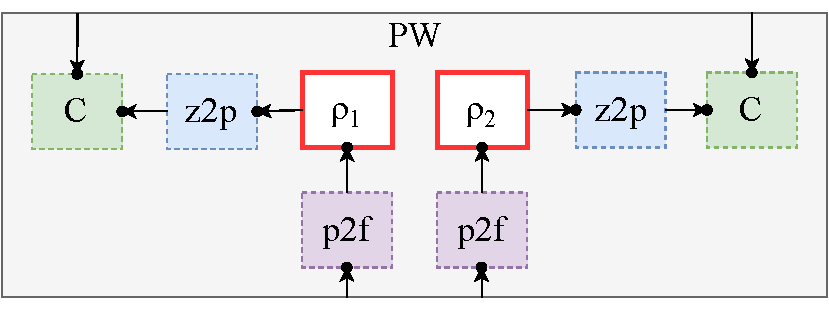
\includegraphics[scale=0.5]{figures/blankpartywrapper2.pdf}
\caption{The internals of the protocol wrapper with two parties. The arrows indicates the client/provider relationship between each pair: provider $\rightarrow$ client. The wrapper creates \texttt{z2p} to offer a channel and convert from gunctional to message type---the \texttt{p2f} do the same. A communicator is used because \texttt{z2p} cannot send message to real one with differing token type. The types of the processes offered are (color): \tgr{comm[z2pmsg[comp2f]]}, \tb{sender}, \tr{party[Int]}, \tp{comm[p2fmsg[rop2f]]}. }
%The processes \texttt{z2p} offer linear channels to their respective protocol parties that are typed according to that party's protocol, and they receive messages from virtual communicators that hold messages specific to one \texttt{pid}. The protocol code for $\pi_1$ and $\pi_2$ are user-specified and offer a channel to the \texttt{p2f} process according to their protocol with the functionality. The \texttt{p2f}s convert outgoing messages to, and incoming messages from, functional message types to be sent to/from the functionality. The protocol wrapper gives messages to the virtual communicators and receives messages from \texttt{p2f}s.}
\label{fig:blankpartywrapper}
\vspace{-1.5em}
\end{figure}

%For the commitment example, if $\pi_1$ and $\pi_2$ ran the commitment protocol, \inline{z2p} would offer a channel of type \inline{sender} and \inline{receiver} to $\pi_1$ and $\pi_2$, respectively, and it converts between the functional messages for the commitment protocol and the session typed ones. 
%In the ideal world, the $\pi_1$ and $\pi_2$ run a dummy protocol where their offered channels are simply forwarded to their \inline{z2p} channels, i.e. the \inline{z2p} and \inline{f2p} channels have the same type: \inline{sender} and \inline{receiver}, respectively.
%In the style of Nomos, the protocol wrapper:
%\begin{itemize}
%	\item Attempts to read messages incoming from \Z, \A, or \F and forward them to the appropriate process depending on \inline{pid}.
%	\item Read from the internal communicators or the \inline{p2f} processes for outcoing messages.
%\end{itemize}
%For reference the functional messages typed for the commitment protocol are:

%Recall the session types for the sender and receiver, with \Fcom, introduced in Section \ref{subsec:idealcommitment}.
%%\begin{gather}
%%	\mi{stype} \; \m{sender} = \ichoice{\mb{commit} : \m{bit} \product \m{scommitted}} \\
%%	\mi{stype} \; \m{scommitted} = \ichoice{\mb{open} : 1} \\
%%	\mi{stype} \; \m{receiver} = \echoice{\mb{commit} : \m{rcommitted}} \\
%%	\mi{stype} \; \m{rcommitted} = \echoice{\mb{open} : \m{bit} \arrow \one}
%%\end{gather}
%At the beginning there are no parties. When the \A or \Z write to a party with some pid $p$ the protocol wrapper creates $p$ if it does not exist.
%It creates and stores the session-typed channels or all of the parties in channels corresponding to their type and moves channels between them as the type evolves.
%For example for parties' channel with \Z the protocol wrapper generates the following lists:
%\begin{gather}
%	\m{R1L1}[\m{sender}] \\
%	\m{R1L2}[\m{scommitted}] \\
%	\m{R2L1}[\m{receiver}] \\
%	\m{R2L2}[\m{rcommitted}] 
%\end{gather}
%At the beginning of the protocol, the committer's \msf{z2p} channel would be in \inline{R1L1} and the receiver's is in \inline{R2L1}.
%The channel's connection the protocol wrapper to the rest are still functionally typed. It's channel \inline{p2f} will still be typed \inline{#ptof: comm[p2fmsg[comp2f]]} where \inline{comp2f} is:
%Succinctly, the protocol wrapper functions as follows:
%\begin{itemize}
%\item When the protocol wrapper receives a message for some \msf{pid}, if the party doesn't exist the protocol wrapper creates all the party's channel parameterized by the correct session types (the role of the party is determined by the incoming message). The channels are stored and outgoing channels are waiting to be read from.
%\item The message sent to the party with the session type is determined by the functional type. The wrapper creates a session-typed message and forwards the contents of the message to the party.
%Despite accepting functionally typed messages, the protocol wrapper uses session types in this way to allow the type checker to catch invalid and out of order environments, adversaries and functionalities. 
%For example, in the commitment protocol when the committer tries to commit a bit in \Fcom like this:
%\begin{lstlisting}[basicstyle=\small\BeraMonottFamily, frame=single, mathescape]
%$\$$p2f.commit 
%$\tb{send}$ $\$$p2f b
%$\tb{pay}$ {p2fn} $\$$p2f
%\end{lstlisting}
%\begin{lstlisting}[basicstyle=\small\BeraMonottFamily, frame=single, mathescape]
%$\$$p2f.SEND 
%$\tb{send}$ $\$$p2f pid 
%$\tb{send}$ $\$$p2f Commit(b)
%$\tb{pay}$ {p2fn} $\$$p2f
%\end{lstlisting}
%The party wrapper intercepts and converts it to a functionally typed message:
%\item For outgoing messages, the protocol wrapper does a similar conversion where it reads the sesion typed channel output by the party and converts its message to the appropriate functional message type.
%\end{itemize}

%\paragraph{Functionality Wrapper}
%The \fwrapper adopts a similar approach to the \partywrapper, except it only creates one instance of the underlying functionality.
%For the same reason as the \partywrapper, we use an \fwrapper to enable a dynamic set of parties.
%One caveat in supporting such functionalities, is that, so far, only functionalities whose type follows a specific form are allowed.
%In the random oracle type given below, notice that the type before and after a party interacts with it is the same: type $\m{party}[a]$.
%\begin{mathpar}
%\m{party}[a] = \textcolor{red}{\getpot^1} \ichoice{\mb{hash} : \m{pid} \arrow \m{int} \product \m{hashing}[a]} \\
%\m{hashing}[a] = \echoice{\mb{shash} : \m{pid} \arrow \m{int} \product \textcolor{red}{\paypot^0} \m{party}[a]} 
%\end{mathpar}
%A party queries a $\mb{hash}$ of an integer from \Fro and receives an integer as a response. The session type includes the \inline{pid}, which enables it to handle all parties over the same channel.
%
%An example of the internals of the \fwrapper are showing on the left-hand-side of Figure~\ref{fig:multisession}.
%Like the \inline{z2p} processes in the \partywrapper, \inline{S} and \inline{R} represent the sender and receiver in the commitment protocol, and they read from their virtual communicators and communicate with \Fcom over a session-typed channel.

%When a party invokes \Fro, the type it expects is \inline{party[a]}, and when it has received its hash the type is again back at \inline{party[a]}. 
%The wrapper handles such dynamic functionalities by channeling all party communication through one linear channel in the wrapper. 
%Therefore, \Fro reads on one channel and responds to the specific party with some \inline{pid}, and the protocol wrapper remains unchanged. 
%
%The constructions of the protocol wrapper and functionality wrapper enable users to write very simple ideal functionality and protocol code, as we will discuss in the next Section and in the Appedix.

%In the commitment example, \Fcom accepts two channels, one from each party, and two processes are created (call then \inline{p2f} for now) which offer channels of type \inline{sender} and \inline{receiver}, respectively. 
%The wrapper differs from the protocol wrapper for certain functionalities that accept a dynamic number of parties. 
%Continuing with our commitment example, the random oracle functionality, an idealized hash function, is used in the real world to realize \Fcom, and it allows a dynamic set of parties to inteact with it.
%Its session type with protocol parties is given below.
%The session type is special in that, for every interaction, the channels type always ends up back at \inline{party[a]} before any other party tries to use \Fro.
%NomosUC enables ideal functionalities whose types work like this by adding the \inline{pid} to the type, and having only one process in the functionality wrapper offering a channel of this type to \Fro.
%Unlike \Fcom where new communicator and \inline{p2f} process is created for each new party, messages from all parties pass through one such process.
%Additionally, moving the \inline{pid} into the session type means that the protocol wrapper can create arbitrarily many \inline{pid}s to communicate with \Fro.

\paragraph{The Adversary}
The adversary, much like the environment, is providing input to the protocol and functionalities.
As the UC framework is concerned with modular construction for protocols, and NomosUC with using session types to aid in suc construction, we do not give adversaries session types.
Therefore, they are not wrapper like protocols and functionalities, and communicate with all other processes directly through functional message types.

\subsection{Polynomial Bound}
The security of the UC framework relies on computational constraints on adversaries, and, generally, on what all ITMs can do.
It introduces the concept of import tokens as a new way to reason about ITMs being polynomial in the security parameter $k$. 
The import mechainsm as described in UC, and which we descrive in Section~\ref{sec:background}, ensures that a single ITM's execution is upper-bounded by some poynomial $T(n,k)$ where $T$ is a polynomial, $n$ is its net import token balance (received - sent), and $k$ is the security parameter.
Canetti et al. limit their discussion to parameterized systems where all machines do not do anything until they have received at least $k$ import.
We depart from this notion slightly and express ``interactive polynomial time'' by using a bounding polynomial in both import and $k$.
We do this for two reasons.
First, it remedies our exclusion of ``parameterized systems'' by easing the import requirements of cacnonical cryprograpic operations, such as a random oracle operation on $k$-bit strings that would otherwise require $k$ import. 
Second, we add $k$ to reflect a more natural notion of import and modularity in UC by allowing minimial import for constant-work one-shot processes like \Fcom which no longer need import just to handle $k$-bit strings.

In NomosUC, we build import into the type system to be able to reason about ITMs being locally polynomial time given some polynomial $T$.
Specifically, the system provides novel constructs to exchange import, generate potential from that import, and create virtual import for simulating other machines.
%Specifically, the type system can check whether a given polynomial bound in the import amount satisfies the potential generated/used by an open Nomos term.
The language additionally encodes the computational cost of each operation performed by an ITM, and statically guarantees that the execution cost of each ITM is locally polynomial in the net import it has over its entire execution. 
The locally polynomial invariant can be extended to claim that the entire UC execution of locally PPT ITMs is also PPT.

\begin{ddef}[PPT in $k$]\label{def:ppt}
A term $e(k,r)$ is \emph{well-resource-typed} and PPT if, given some amount of initial import $n$, there exists a polynomial $T(n,k)$ such that $\forall k, r, e(r,k) \{n\}$ terminates in at most $T(n,k)$ steps. 
\end{ddef}

%\begin{proof}
%The Nomos type system only type checks programs for which a satisfying assignment of polynomial $T$ is possible.
%Given an $n \in poly(k)$, all programs that type check must be \textit{well-resource-typed.}
%%The Nomos type system guarantees that a satisfying assignment of $n$ and $T$ will correctly type-check.
%%Therefore, given an initial amount of import $n(k) \in poly(k)$, the existence of some $T$ ensures that any process, regardless of its randomized execution according to the bit sequence $r$, $e$ is guarantees to be upper-bounded by $poly(k)$ satisfying the definition of probabilistic polynomial time in $k$.
%\end{proof}

%We demonstrate that our local PPT definition implies a PPT UC execution by adapting Proposition 7 from the UC framework to the NomosUC setting.
%Our sandboxing mechanism and \inline{withdrawTokens} procedure let us simulate the well-resource-typed ITMs, in the UC execution, within one ITM.
%We need only provide a suitable ``exchange rate function'' \GlobalF and a bounding polynomial $T$ on the single machine to conclude that it is well-resource-typed.
%If the initial import given to the system is $n$ then the single ITM generates $n$ virtual tokens, and simulates all inputs generated by the environment.
%Subsequently a sufficient bounding polynomial for this ITM is to the order of $O(n \times T')$ wher $T'$ is the largest polynomial among those bounding the simulated machines. The additional factor of $n$ exists to allow for routing/handling of messages between simulated machines.
%Clearly, this is not a tight bound but it will bound the entire UC execution, and our \inline{withdrawTokens} rules ensures that we are left with a valid token context.
%Therefore, the resulting UC execution, as a single ITM, is also well-resource-typed.

The soundness of our polytime notion comes down to showing that our UC experiment is PPT in only the security parameter $k$. 
The UC framework provides a simulation of a configuration of ITMs on a universal turing machine and proves that such a turing machine is also bounded by a polynomial $T$. 
Given the initial input of import tokens into the machine ($poly(k)$ amount of import), it can conclude that their import mechanism falls in line with the standard notion length-of-input polynomial time and satisfied their ``PPT in $k$'' definition. 
In NomosUC, we do not deal directly with ITMs, however, our type system allows us to judge whether a process, or collection of processes through the Preservation Theorem~\ref{thm:preservation}, is locally PPT given a particular polynomial. 
We use this judgement as a foundation and adapt Proposition 7 from UC~\cite{uc} to NomosUC, and show that our notion of locally PPT leads to a UC execution that is PPT in the security parameter $k$.

\todo{Define \F, \A, \Z, \m{PW}(\PI) as configurations that include the communicators to be used. Just need to create a standard for which direction communicator is part of which configuration.}
\begin{theorem} \label{thm:soundness}
Let \F, \A, \Z, and \m{PW}(\PI) be locally PPT configurations bounded by super additive polynomials $T_\F$, $T_\A$, $T_\Z$, $T_\PI$. Let \m{UC} be a configuration composed of a single process that runs \inline{execUC},. If \m{UC} receives $n \in poly(k)$ import initially, then the composed configuration $\m{UC} = \m{execUC} \; || \; \Z \; || \; \A \; || \; \m{PW}(\PI) \; || \; \F$ is PPT in $k$, where \m{PW} is the \partywrapper.
\end{theorem}

\begin{proof}
The resulting configuration \m{UC} has only one channel in it's context: the channel offered by \inline{execUC} of type \inline{Bit}. 
\inline{execUC}, therefore, is the intial process in the configuration and receives the intial import $n \in poly(k)$.

By the \m{compose} rule, the work done by the resulting configuration is strictly the sum of the work done by the composed configurations. 
The Preservation Theorem in conjunction with \m{compose} ensures type safety of \m{UC}, and allows us to concluce a sufficient bound on the total work done in \m{UC} by the polynomial $T'(n,k) = T_\A(n,k) + T_\Z(n,k) + T_\P(n,k) + T_\F(n,k) + O(1)$ where $n$ is the initial import into the system, and the addition $O(1)$ accounts for the constant bound on \inline{execUC}.
If we take the intial import $n$ to be polynomial in the security parameter $k$, we conclude that \m{UC} is PPT in $k$.
\end{proof}

\paragraph{Sending/Receiving Import}
Our construction of the UC experiment requires communicators (introduced in Section~\ref{sec:nomosuc}) to intermediate communication between the \Z, \A, \F, and \m{PW}(\PI).
Their use adds import requirements to the experiment that are not captures by just the types of \F, \A, and \PI. 
It results from them being activates a potentially polynomial number of times. Therefore, the communicator's type, introduced in Section~\ref{sec:nomosuc} defines the, reflects this computation by
retaining one of the import tokens that is sent accross it. 
Given that our functionalities are parameteric in the amount of import they send/receive (so as to not restriction wat protocols can realize them), the user must take into account the number of import taken by communicators.
In our commitment example, the messages from \Z that uses the most import in the real world is the sending the \inline{open} message to the committer. This activationa results in 5 communicators being activated and so five more import than the protocol already requires. As long as the ideal functionality is parameterized to accept the same amount of import, indistinguishability still holds. \todo{This belongs somewhere else}.

%Our construction of the \partywrapper and \fwrapper rely on sending functional messages between them through a shared communicator.
%The same holds true between the adversary and the two wrappers, and also holds true between the environment and the \partywrapper.
%When any of these parties is sending import to each other, they must always send the maximum import of any message that can be exchanged with each other.
%For example if parties $p_1$ and $p_2$ send $n_1$ and $n_2$ import to the functionality, then the communicator between the \partywrapper and \fwrapper will be typed to expect $max(n_1, n_2)+1$ import on every message from the \partywrapper and vice versa for messages from \fwrapper to \partywrapper. 
%Recall from Section~\ref{sec:nomosuc} that the $+1$ is required to give the communicator at least one unit of import.
%Similarly, \Z will send the maximum of the imports required by $p_1$ and $p_2$ plus two additional import for communicators.
%In total, for any activation by \A or \Z there can be up to three communicators activated in the execution. 

%An simple example where that illustrates the type system's capabilities is the authenticated append/read functionality $\F_\msf{AppRd}$~\footnote{We provide the code for this functionality in the appendix for the simplified case of a single party.}.
%The functionality requires parties to provide 1 unit of import to append items to the list and 1 unit of import to read from the list, and the functionality generates potential proportional to the length of the list in order to traverse it.
%It is clear that the total work performed by $\F_\msf{AppRd}$ is bounded by a quadratic poynomail, and the NomosUC type system ensures that only bounding polynomials quadratic or larger successfully type check.
%\todo{something more to say here}

%\begin{definition}[PPT Term]\label{def:pptterm}
%A \textit{PPT term} is a \textit{well-typed} term $e(k, r)$ that is \textit{closed} except for security parameter $k$, random bit sequence $r$.
%\end{definition}
%
%We first-define terms that are well-typed in the traditional session-types-sense in Definition~\ref{def:pptterm}, i.e. without any resource constraints~\cite{caires2010session}.
%Such terms are closed except for the security parameter $k$ and some uniformly random bit sequence $r$. 

%However, we also want to reason about terms that are well-typed when connected to another Nomos terms.

\subsection{Emulation}
Emulation underpins the UC security definition, and reasons about indistinguishability between two protocols over all adversaries against it and a simulator for all environments.
In NomosUC, we must be more careful to only consider protocols and adverasaries whose types (both message and import) match over the channels they share. 
Therefore, we introduce the term \textit{well-matched} to mean a PPT term $e$ is well-typed when connected to another term $e'$.
Simply put, we want to capture terms $e$ and $e'$ that can be connected over the channels the share given their type.
The resulting terms in Definition~\ref{def:wellmatched} are partionall closed after connection: the terms may only be connected on some subset of their channels.
%Simply put, the channels that $e$ and $e'$ share are of the same type. 
%Specifically, we want to exclude processes that logically share a channel, say the channel from \inline{p} to \inline{f}, but send (their types message types don't match).
%This new definition becomes important when we discuss UC emulation below as we want to reason about environments that are \textit{well-matched} for a protocol $\pi$ or a specific adversary \A.

\begin{ddef}[Well-Matched]\label{def:wellmatched}
\begin{mathpar}
\footnotesize
\inferrule*[right=Well-matched]
{\Tokens_1, K \semi \Delta_1 \vdash e :: \Delta_1' \semi 
\Tokens_2, K \semi \Delta_2 \vdash e' :: \Delta_2' \\ \\
 S \equiv \Delta_1 \bigcap \Delta_2 \neq \emptyset}
%{\Delta_1 \leftrightarrow \Delta_2}
{\Delta_1 \equiv_{S} \Delta_2 \semi e \leftrightarrow e'} 
\end{mathpar}
\end{ddef}

In the UC security definition, we say that a protocol $\pi$ posesses the same security properties as another protocol $\phi$ if no environment can distinguish between them for any adversary.
In most cases we compare a real protocol $\pi$ with an idealized protocol $(\idealP, \F)$ which is actually just an ideal functionality with dummy parties.
The ideal functionality is known to achieve the desired security processes because it acts like a simple, trusted third party.
%They are much simpler than protocols because they don't require any special code to handle mutually distrustful other processes, and they perform the given computation on behald of the ideal world parties.

Given the random choices ITMs in UC can make, it is clear that the outputs of \inline{execUC} produces and ensemble of distributions over all possible random bitstrings and security parameters.
Emulation, then, is about the ensembles created by two UC environments being computationally indistinguishable from each other.
We define indistinguishabiliy between ensembles in a standard way using \textit{statistical distance} in Definition~\ref{def:distance}.

\begin{definition}[Indisinguishability]\label{def:distance}
Two ensembles $\mathcal{D}_{1,k}, \mathcal{D}_{2,k}$ are indistinguishable, $\mathcal{D}_{1,k} \sim \mathcal{D}_{2,k}$, if their statistical distance is at most $negl(k), \forall k$.
\end{definition}

%\paragraph{Validity}
%For the remainder of this section we refer to \emph{valid} adversaries and simulators given a particular protocol, functionality, or environment.
%We refer to adversaries that type-check when connected to \Z, \F, or $\Pi$ by \inline{execUC}, and that are \emph{well-matched} as defined above. 
%Indisintiguishability between two protocols is defined as follows (we shorten the communicator type \msf{comm} to \msf{c}):

UC emulation combines the UC exeution with indistinguishability resuting in the following NomosUC emulation definition.
\begin{definition}[Emulation]\label{def:emulation}
Given two protocols $(\pi, \F_1), (\phi, \F_2)$ that are well-resource-typed then if $\forall \A$ well-matched with $(\pi, \F_1)$, $\exists \Sim$ s.t. $\forall \Z$ well-matched with \A and $(\pi, \F_1)$: \Sim is well-matched with $(\phi, \F_2)$, \Z is well-matched with $(\phi, \Sim)$, and $\msf{execUC}(\pi, \F_1, \Z, \A) \approx \msf{execUC}(\phi, \F_2, \Z, \Sim)$:

\begin{mathpar}
\footnotesize
	\inferrule*[right=emulate]
	{
		%. \models \msf{execUC}[\Tokentypes][\alpha] :: \Delta[\Tokentypes][\alpha] \\ \\ 
		% Protocols that are well-matched with their functionalities
		%\pi \rightarrow \Delta_1' \semi \phi \rightarrow \Delta_2' \semi \\
		\pi : \Delta_1'[\Tokentypes][\mathrm{T}_{\pi}] \semi \phi : \Delta_2'[\Tokentypes][\mathrm{T}_{\phi}] \semi \\
		%\langle \pi \leftrightarrow \F_2 \rangle, \langle \phi \leftrightarrow \F_1 \rangle \\
		% Type of execUC[DELTA_pi] and execUC[DELTA_phi]
		\forall \A \, | \, \Delta_4[\Tokentypes][\mathrm{T}_{\A}] \vdash \A :: \Delta_4', \langle \A \leftrightarrow \pi \rangle\\
		%\Delta_1'[\Tokentypes][\mathrm{T}_{\pi}] \equiv_{\Z} \Delta_1\ 
		%\semi \Delta_2'[\Tokentypes][\mathrm{T}_{\phi}] \equiv_\Z \Delta_2 \\
		% For all A if exists well-typed A that is well-matched with real world
		%\forall \A, (\exists (\Delta_4, \Delta_4') | \Delta_4 \vdash \A :: \Delta_4', \langle \A \leftrightarrow \pi \rangle, \langle \A \leftrightarrow \F_1 \rangle \\
		%\forall \A | \Delta_4 \vdash \A :: \Delta_4', \langle \A \leftrightarrow \pi \rangle, \langle \A \leftrightarrow \F_1 \rangle \\
		% implies simulator that is well-matched for ideal world
		%\Rightarrow \exists (\Delta_3,\Delta_3') \, | \, \Delta_3 \vdash \Sim_\A :: \Delta_3', \\ % \langle \Sim_\A \leftrightarrow \phi \rangle, \langle \Sim_\A \leftrightarrow \F_2 \rangle \\
		\Rightarrow \exists \Delta_3[\Tokentypes][\mathrm{T}_{\Sim}] \vdash \Sim_\A :: \Delta_3', \langle \Sim_\A \leftrightarrow \phi \rangle \\ % \langle \Sim_\A \leftrightarrow \phi \rangle, \langle \Sim_\A \leftrightarrow \F_2 \rangle \\
		% for all Z they that's well-matched for the real world => Z is well-matched with S and ideal world
		%\forall \Z (\langle \Z \leftrightarrow \A \rangle, \langle \Z \leftrightarrow \pi \rangle \Rightarrow \langle \Z \leftrightarrow \Sim_\A \rangle, \langle \Z \leftrightarrow \phi \rangle \\
		% and emulation has to hold
		\Rightarrow \forall \Z \; \msf{execUC} \ \pi\ \Z\ \F_1\ \A \approx\ \msf{execUC} \ \phi\ \Z\ \F_2\ \Sim_\A
	}
	{
		% EMULATION DEFINITION
		\lambda \A . \Sim_\A \vdash (\pi, \F_1) \sim (\phi, \F_2) % \F_1 \xrightarrow{\pi} \F_2
		%\lambda \A . \Sim_\A \vdash (\pi, \F_1) \sim (\phi, \F_2)
	}
\end{mathpar}
\end{definition}
The emulation definition above is quite straightforward. It starts with defining the protocols in question and their type under the type parameters passed to \inline{execUC}.
It then states that for all adversaries that are well-matched with $\pi$ and $\F_1$, there exists a simulator such that the two executions are indistinguishable. 
The definition ensures that for emulation to hold, the constructed simulator must be well-matched everywhere \A is well-matched: for all environments \A is well-matched with the \Sim must also be well-matched with.

With this emuluation definition we complete our definition of UC-realization in Definition~\ref{def:realize}.
If a simulator exists such that emulation holds for $(\pi, \F_1) \sim (\idealP, \F_2)$ then we say that the protocol $\pi$ UC-realied the functionality $\F_2$ in the $\F_1$-hybrid world:
\[
	\F_1 \xrightarrow{\pi} \F_2
\]

\paragraph{Import for Functionalities}
The \Fcom example use throughough this work is realized by protocol that uses the random oracle. 
A natural notion of import should define \Fcom as requiring 0 import because it is one-shot and halts after doing constant amount of work.
\Fro on the other hand, requires at least 1 unit of import in order to be handle a potentially polynomial mumber of activations as well as reading/writing $k$-bit strings.
This poses a problem that the ideal world requires 0 import however, the real world requires at least 1 unit of import.
We resolve this dilemma by defining functionalities as parameteric in the amount of import they require.
Parametric functionalities do not restrict UC-realization to only those protocols that are as compitatiaonally ``efficient'' as the them. In cryptography, it is common for real protocols to be computationally intensive while the ideal functionality they are realizing is trivial, and we want to be able to express such emulation.
We modify the arrow notation, slightly, to capture that a functionality can realize itself while requiring more import, and use the notation $\F^m$ to denote a functionality parameterized to require $m$ import.
\[
	\F_1^m \xrightarrow{\idealP} \F_2^{n \geq m}
\]
For the remainder of this work we do not bother import annotations on functionalities and only concern ourselves with the minimum import they require because it is an implementation detail.

%When we talk about emulation, we particularly care about emulation with respect to an ideal protocol $\phi$ which is really just $(\idealP, \F)$ where \idealP is the protocol which forwards all messages to/from \Z and \F.
%We say the protocol $\pi$ (potentially with a hybrid functionality $\F_1$) UC-realizes an ideal functionality $\F_2$ if Definition~\ref{def:emulation} holds for $(\pi, \F_1)$ and  $\phi = (\idealP, \F_2)$

%\begin{definition}[UC-Realize]
%A protocol $\pi$ UC-realized an ideal functionality $\F_1$ if $(\pi, \F_2) \sim (\idealP, \F_1)$ for some $\F_2$.
%
%\begin{mathpar}
%\footnotesize
%\inferrule*[right=UC-Realize]
%{ (\pi, \F_1) \sim (\idealP, \F_2) }
%{ \F_1 \xrightarrow{\pi} \F_2 }
%\end{mathpar}
%\end{definition}

\subsection{Dummy Lemma} \label{sec:dummy}
The dummy lemma is a crucial result in UC that reduces the design space of simulators to just one: for the dummy adversary in the real world.
The Lemma states that if a simulator exists for the dummy adversary, called the dummy simulator \DS, then there it is easy to construct a simulator for any other adversary \A. 
The simulator constructed in this lemma uses virtual tokens to internally run \DS and \A.

The intuitiom behind this results rests in the fact that emulation must hold over $\forall \Z$ for a particular \A. 
Particularly, in the case of \DS and \DummyAdv, emulation holds for a \Z that may be running any other possible \A internally and passing it's output to \DS and \DummyAdv.
Therefore, moving \A out of the simulation and into the execution, as the real adversary and as providing input to \DS, should maintain emulation between the two worlds.

\begin{theorem}[Dummy Lemma]\label{thm:dummy}
If \ $\exists \DS$ s.t. $ \DA, \DS \vdash \F_2 \xrightarrow{\pi} \F_1$ then $\forall \A \ \exists \Sim_\A$ s.t. $\Sim_{\A} \vdash  \F_2 \xrightarrow{\pi} \F_1)$ 
\end{theorem}

We give the proof of this lemma in the appendix, however, we provide an intuition for understanding why it is true.
Simulation w.r.t the dummy simulator works for all environments, even those that could run any potential real-world adverasry internally. Such environments, pass input to the adversary, whose output is given to the dummy simulator. 
The constructed simulator captures the idea of moving the adversary from the environment into the the execution, and the constructed simulator runs the real-world adverasry and dummy simulator internally.
Environment inputs are not passed to the adversary, and the adversary's outputs are passed to the dummy simulator.

%\begin{proof}
%The constructed simulator $\Sim_\A$ internally simulates \DS and \A through a virtual token type $K'$. 
%We describe the simulation pattern below to simulate messages to \DS and \A.
%
%On \inline{Z2A2P} input from \Z on channel \msf{z2a}, \Sim fowards the message to the internal \A with the same type but virtual tokens instead of real ones:
%\begin{lstlisting}[basicstyle=\small\BeraMonottFamily, frame=single,  mathescape, label={lst:sim}]
%msg = $\nrecv$ $\$$z2a ;
%$\nget$ $\$$z2a {z2an : K} ;
%$\tm{withdrawTokens}$ f K K1 z2an ;
%$\nsend$ $\$$a_z2a msg ;
%$\npay$ {z2an : K1} $\$$a_z2a ; 
%\end{lstlisting}
%
%Similarly, on \inline{A2P(pid,msg)} output from \A to a protocol party on channel \msf{a2p}, \Sim sends the message to \DS as input from \Z (type: \inline{Z2A2P(pid, msg)}:
%\begin{lstlisting}[basicstyle=\small\BeraMonottFamily, frame=single,  mathescape]
%pid = $\tb{recv}$ $\$$a_a2p ;
%msg = $\tb{recv}$ $\$$a_a2p ;
%$\tb{get}$ K1 $\$$aa2p {a2pn} ;
%$\tb{send}$ $\$$sd_z2a A2P(pid, msg) ;
%$\npay$ $\$$sd_z2a {z2an : K1} ;
%\end{lstlisting}
%
%$\Sim_\A$ accepts input from \Z and forwards it to the internal \A, which outputs to either the protocol parties or the ideal functionality. 
%\Sim forwards this output to \DS acting as input from the environment  and forward any outputs \DS creates to the intended recipients.
%Our main proof obligation here is to ensure that $\SIM{\A}$ in NomosUC is well-resource-typed for all well-resource-typed \A.
%The $\Sim_\A$ performs constant overhead on the simulattion of \A and \DS. Therefore, a sufficient bounding polynomial on the runtime of $\Sim_\A$ can be given as:
%\[
%T(n) = T_{\A,\DS}(n) + T_{\A,\DS}(n) + O(n)
%\]
%where $T_{\A,\DS}(n)$ is the greater of the two bounding polynomials for \DS and \A evaluated at $n$, and $n$ is the import that \Z sends to \A and \Sim. 
%We must also reason about the use of virtual tokens.
%Given that \A and \DS are well-resource-typed we can conclude that the virtual import tokens generated for activating \A and \DS never exceeds a polynomial in the number of real import tokens received by \Sim. 
%\end{proof}

\subsection{Single Composition}
In this section we present a composition operator for protocols that completes the single composition theorem, Theorem~\ref{thm:singlecomp}.
The composition operator allows replacement of a functioality with a protocol realizing it, and, potentially, any functionality that protocol uses.

Say a protocol $\pi$, using hybrid functionality $\F_1$, realizes functionality $\F_2$. 
For a protocol $\rho$ that uses $\F_2$, replacement results in parties of $\rho$ being directly connected to parties of $\pi$ within the \partywrapper.
The protocol party $\rho_i$ that is connected to its \inline{p2f} process with a channel of type $\mb{a}$ is connected to party $\pi_i$ with the same channel.
Party $\pi_i$ is, in turn, then connected to its \inline{p2f}.
This replacement is visually described in Figure~\ref{fig:replacement}.

%In this section we present a simplified composition theorem and a second theorem we call the squash theorem.
%These two theorems combine later in the section to prove the full UC composition theorem as it appears in the UC framework~\cite{uc}.
%
%Briefly the composition operator allows substitution of a functionality for a protocol that realized is. 
%The theorem states that a protocol that uses some functionaliy \F can replace with a protocol $\pi$ that realizes it along with any hybrid functionality $\pi$ uses.
%More specifically, in NomosUC, say a protocol $(\pi, \F_1)$ realizes some functionality $\F_2$.
%A protocol $\rho$ that uses $\F_2$ can replace is with instances of $\pi$ directly connected to the corresponding instances of $\rho$ \emph{within} the protocol wrapper, and the ideal functionality $\F_2$ being replaced by $\F_1$ in the functionality wrapper.

%We highlight first, that our protocol wrapper construction illustrated in \ref{fig:blankpartywrapper}, connects the internal process in that specific way to enable composition.
%Recal that the Nomos language has the concept of clients and providers for a give linear channel. Given to processes, the type of the channel changes depending on which process \emph{offers} the channel, i.e. is the provider, and who is the client.
%The arrows in Figure~\ref{fig:blankpartywrapper} illustrate the \emph{client} $\rightarrow$ \emph{provider} relationship.
%We illustrate how protocol replacement works in NomosUC in Figure~\ref{fig:replacement}.

\begin{figure}
\centering
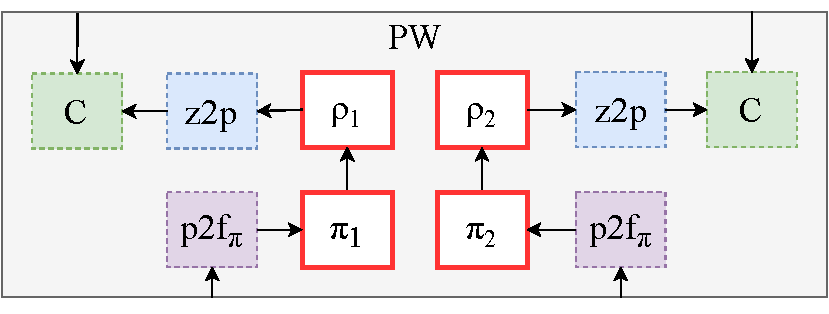
\includegraphics[scale=0.5]{figures/replacement2.pdf}
\caption{When we compose protocols we replace the \emph{p2f} process of $\rho$ with the corresponding instance of $\pi$ and its \emph{p2f} processes. By the emulation theorem, the channel offered by $\rho$ and accepted by $\pi$ have the same type.}
\label{fig:replacement}
\end{figure}

The code for the operator has the same type as any other protocol except, from the description above, it's offered channel is for the type of the functionality $\F_1$ instead of $\F_2$.
We rely on the code generation for to handle spawning instaces of a \inline{p2f} process corresponding to $\pi$ rather than $\rho$.
The operator is given in Figure~\ref{lst:compose}.
\begin{figure}
\begin{lstlisting}[basicstyle=\footnotesize\BeraMonottFamily, frame=single, mathescape]
$\tb{proc}$ compose[K][z,p]:
  (pid: Int), (rng: [Bit]), (sid: session[1]),
  (pid: Int), ($\$$z2p: z) |- ($\$$c: p) =
{
  $\$$ch <- PS.rho <- k rng sid pid $\$$z2p ;
  $\$$c <- Ps.pi <- k rng sid pid $\$$ch 
}
\end{lstlisting}
\caption{The composition operator accepts the same parameters as any other protocol party and offers the channel of type $p2f$ of the realizing protocol $\pi$. We connect $\rho$ to $\pi$ as an environment giving input to $\pi$. We do not need to include any import in our composition operator as the two protocols are guaranteed to be well-matched by the emulation definition. The operator replaces only one party (one \msf{pid}), and the \partywrapper instantiates parties that run the composed protocol.}
\label{lst:compose}
\end{figure}

The resulting composition operator, which composes the two simulators \SIM{\rho} and \SIM{\pi} inside the construction simulator, is best described in text as the resulting code is too verbose to include in the main body of this paper.
You can find the full simulator composition operator in the appendix.
\begin{itemize}
	\item Input from \Z is split between the two simulators
	\begin{itemize} 
		\item \inline{Z2A2P(pid, msg)} intended for parties of $\rho$ are passed to \SIM{\rho}
		\item \inline{Z2A2F(msg)} intended for $\F_1$ is passed to \SIM{\pi}.
	\end{itemize}
	\item Output from \SIM{\pi}: 
	\begin{itemize}
		\item \inline{A2F(msg)} for $\F_2$ and \inline{A2P(pid,msg)} for dummy parties of $\F_2$ are sent to \SIM{\rho} as \inline{Z2A2F(msg)}
		\item \inline{F2A2Z(msg)} is sent to \Z unaltered.
	\end{itemize}
	\item Output from \SIM{\rho}: 
	\begin{itemize}
		\item \inline{A2F(msg)} and \inline{A2P(pid,msg)} for $\F_3$ are sent out unaltered.
		\item \inline{F2A2Z(msg)} messages are sent to \SIM{\pi} as \inline{F2A(msg)} from $\F_2$.
		\item \inline{P2A2Z(pid,msg)} messages are sent to \Z unaltered.
	\end{itemize}
\end{itemize}
The simulator relies on simulators for $\F_1 \xrightarrow{\pi} \F_3$ and $\F_2 \xrightarrow{\rho} \F_3$ to satisfy simulation for Theorem~\ref{thm:singlecomp}.
It is clear that this construction adequately simulates the composed protocol. 
The type in the ideal world gurantees that both the real and ideal world adversaries get at least as much impor as any of the protocol parties. 
This ensures that the composed simulator has enough import to sandbox the two existing simulators and send import out to the ideal world parties and ideal funfctionality.
Therefore it is trivial to see that the composed simulator is well-resource-typed.

Another illustrative description of what composition proposes, logically, is shown by this series of UC executions where the $\equiv$ operator denotes equivalent UC executions that result from moving ITMs in and out of a sandbox, and $\approx$ indicates emulation:
\begin{align}
& \msf{execUC} \: \Z \, (\rho \circ \pi) \, \F_1 \, \DA \\
\equiv \; & \msf{execUC} \: (\Z \circ \rho) \, \pi \, \F_1 \, \DA \\
\approx \; & \msf{execUC} \: (\Z \circ \rho) \, \idealP \, \F_2 \, \SIM{\pi} \\
\equiv \; & \msf{execUC} \: \Z \, \rho \, \F_3 \, (\SIM{\pi} \circ \SIM{\rho})
%\approx \; & \msf{execUC} \: (\Z \circ \Sim{\pi}) \, \idealP \, \F_3 \, \Sim{\rho} \\
%\equiv \; & \msf{execUC} \: \Z \, \idealP \, \F_3 \, (\Sim{\pi} \circ \Sim{\rho}) 
\end{align}

%\item Inputs from \Z of \inline{Z2A2P(msg)} are passed to \SIM{\rho}, and inputs of \inline{Z2A2F(msg)} are passed to \SIM{\pi}.  
%\item \inline{P2A2Z(pid, msg)} outputs from \SIM{\rho} are forwarded to \Z unaltered.
%\item \inline{A2F(msg)} and \inline{A2P(pid, msg)} messages from \SIM{\pi} for $\F_2$ are sent to \SIM{\rho} as \inline{Z2A2F(msg)} and \inline{Z2A2P(pid, msg)}, respectively. 
%\item In the reverse direction, \inline{F2A2Z(msg)} messages from \SIM{\rho} are sent to \SIM{\pi} as \inline{F2A(msg)}, and, finally, \inline{F2A2Z(msg)} output generated by \SIM{\pi} is forwarded to \Z.
%\item \inline{A2P(pid,msg)}, \inline{A2F(msg)} messages from \SIM{\rho}, and \inline{P2A(pid,msg)} and \inline{F2A(msg)} from $\F_3$, are forwarded unaltered. 
%\end{itemize}

%We also provide a composition operator for simulators to construct a simulator for the composed protocol. We connect the simulatorsin the following way
%\begin{figure*}
%\begin{lstlisting}[basicstyle=\small\BeraMonottFamily, frame=single, mathescape]
%$\tb{proc}$ sim_compose[K][a2r,r2a][a2p,p2a][a2f,f2a]:
%  (k: Int), (rnd: [Bit]), (sid: session[1]),
%  (#z_to_a: comm[z2amsg[a2r][a2f]]), (#a_to_z: comm[a2zmsg[r2a,f2a]]),
%  (#a_to_p: comm[a2pmsg[a2r]]), (#p_to_a: comm[p2amsg[r2a]]), (#a_to_f: comm[a2fmsg[a2f]]), (#f_to_a: comm[f2amsg[f2a]])
%    |- ($\$$c: 1) =
%{
%  $\$$ch 
%\end{lstlisting}
%\end{figure*}

%\begin{figure*}
%\begin{lstlisting}[basicstyle=\small\BeraMonottFamily, frame=single,  mathescape]
%$\tb{proc}$ compose[K][z2r][r2z][f2r][r2f][p2f][f2p] : 
%    (pid: Int), ($\$$z_to_p: c[K][z2p]), ($\$$p_to_z: c[K][r2z]), 
%    ($\$$f_to_p: c[K][f2r]), ($\$$p_to_f: c[K][r2f])  |- ($\$$D : 1) =
%{
%	$\$$rho_to_pi <- $\tm{createchan}$[K][p2f];
%	$\$$pi_to_rho <- $\tm{createchan}$[K][f2p];
%
%	 <- pi  <-                 $\$$rho_to_pi $\$$pi_to_rho $\$$p_to_f $\$$f_to_p ;
%	 <- phi <- $\$$z_to_p $\$$p_to_z $\$$rho_to_pi $\$$pi_to_rho ; 
%}
%\end{lstlisting}
%\caption{Composition operator in Nomos that connects a protocol $\rho$ to a protocol $\pi$ that uses some functionality $\F$. The operators creates new channels to connect the realizing $\pi$ and it's hybrid \F. Output from $\rho$ intended for the replace functionality are actually send to parties of $\rho$, and channels outgoing from the parties to the functionality are given to $\pi$.}
%\label{lst:compose} 
%\end{figure*}

%\begin{theorem}[Composition]\label{thm:singlecomp}
%\begin{mathpar}
%\inferrule*[right=single-compose]
%{
%	\F_1 \xrightarrow{\pi} \F_2 \semi \F_2 \xrightarrow{\rho} \F_3 \\
%}
%{
%	\F_1 \xrightarrow{\rho \circ \pi} \F_3
%}
%\end{mathpar}
%
%If \textit{well-typed} $(\pi, \F_1$) realizes $\F_2$ and ($\rho$, $\F_2$) realizes some $\F_3$, then $(\rho \circ \pi, \F_2)$ is \textit{well-typed} and realizes $\F_3$ when $\circ$ is defined as in Figure~\ref{lst:compose}.
%\end{theorem}

%\begin{proof}
%The pre-condition ensures the existence of \textit{well-resource-typed} simulators $\Sim_\rho$ for $\F_2 \xrightarrow{\rho} \F_3$ and $\Sim_\pi$ for $\F_1 \xrightarrow{\pi} \F_2$, and, it is obvious that the composed protocol is also well-resource-typed.
%We construct a simulator \Sim' for the dummy adversary to show
%\[
%	\msf{execUC}\ (\rho \circ \pi)\ \F_1\ \Z\ \A \approx \msf{execUC}\ \idealP\ \F_3\ \Z\ \Sim''
%\]	
%
%The simulator $\Sim'$ relies only simulating \SIM{\pi} and \SIM{\rho}.
%Note that \SIM{\pi} can accept messages for $\pi$ or $\F_1$, simulate them, and generate input for $\F_2$. 
%Similarly, \SIM{\rho} can take inputs for $\rho$ or $\F_2$, simulate them, and generate input for $\F_3$.
%Therefore, we connect the two simulators in the natural way:
%\begin{itemize}
%\item Inputs from \Z of \inline{Z2A2P(msg)} are passed to \SIM{\rho}, and inputs of \inline{Z2A2F(msg)} are passed to \SIM{\pi}.  
%\item \inline{P2A2Z(pid, msg)} outputs from \SIM{\rho} are forwarded to \Z unaltered.
%\item \inline{A2F(msg)} and \inline{A2P(pid, msg)} messages from \SIM{\pi} for $\F_2$ are sent to \SIM{\rho} as \inline{Z2A2F(msg)} and \inline{Z2A2P(pid, msg)}, respectively. 
%\item In the reverse direction, \inline{F2A2Z(msg)} messages from \SIM{\rho} are sent to \SIM{\pi} as \inline{F2A(msg)}, and, finally, \inline{F2A2Z(msg)} output generated by \SIM{\pi} is forwarded to \Z.
%\item \inline{A2P(pid,msg)}, \inline{A2F(msg)} messages from \SIM{\rho}, and \inline{P2A(pid,msg)} and \inline{F2A(msg)} from $\F_3$, are forwarded unaltered. 
%\end{itemize}
%It is clear that \Sim' is able to emulate inputs from \Z to both parties of $\rho$ and the ideal functionalty $\F_1$.
%\Sim' performs constant over head in simulating two \emph{well-resource-typed}, and therefore it is clear that \Sim' is \emph{well-resource-typed}.
%When combined with the \emph{dummy lemma}, a well-resource-typed simulator exists for composition for any adverasry \A. 
%The dummy lemma presented above ensures that a simulator for any \A can be constructed that is well-resource-typed for all wel-resource-typed \A.
%\end{proof}
%
%We give a simpler, high-level idea of the forst step of the proof proof here which can be understood visually:
%The $\equiv$ operator is a result of moving around ITMs (some from within other ITMs into the main UC execution) and $\sim$ refers to indistinguishability.
%In line (13) above, $\rho$ is moved into the execution environment with an unchanged simulator as no additional simulation is required: the simulator allows unfettered communication between parties of $\rho$ and \Z.

\subsection{Multisession}

\begin{theorem}[Composition]\label{thm:composition}
\begin{mathpar}
\inferrule*[right=compose]
{
	%(\pi, !\F_1) \sim (\idealP, F_2) \semi (\rho, !\F_2) \sim (\idealP, \F_3) \\ 
	!\F_1 \xrightarrow{\pi} \F_2 \semi !\F_2 \xrightarrow{\rho} \F_3 \\
	%\Rightarrow \exists \Sim(\A) \vdash (\rho^{!\F_2 \rightarrow (!\pi \, \circ \, \msf{squash})}, !\F_1) \sim (\idealP, \F_3)
}
{
	!\F_1 \xrightarrow{\rho \, \circ !\pi \circ \, \msf{squash}} \F_3
	%(\rho \, \circ \, !\pi \circ \msf{squash}, !\F_1) \sim (\idealP, \F_3)
}
\end{mathpar}
\end{theorem}
Full composition in the UC framework extends beyond the simpler composition in Theorem~\ref{thm:singlecomp} which only defines replacement of one functionality with a protocol that realizes it.
Instead, UC composition allows for replacement of any number of instances of a functionality with instancesof the realizing protocol.
Theorem~\ref{thm:composition} illustrates the full composition theorem using our arrow notation, and highlights a theorem that we must prove before we can achieve full composition.
It relies on Theorem~\ref{thm:squash} that introduces the \msf{squash} protocol and the $!$ operator.
Notice that Theorem~\ref{thm:compose} follows directly from Theorem~\ref{thm:singlecomp} and Theorem~\ref{thm:squash}.

The multi-session extension of a protocol or functionality, specified by the $!$ operator (such as $!\rho$ or $!\F$), allows multiple instances of the protocol/functionality to be run within a sinlge ITM.
An ITM simulates the instances and multiplexes input/output to/from them much like the \partywrapper.

\begin{theorem}[Squash Theorem]\label{thm:squash}
%If a functionality \F is well-resource-typed, then $!\F$ and $!!\F$ are well-resource-typed (by Theorem~\ref{thm:bangppt}) and $(\idealP, !!\F) \sim (\msf{squash}, !\F)$.
%\textit{Well-resource-typed} \F $\Rightarrow$ $!\F \xrightarrow{\msf{squash}} !!\F$%  $(\idealP, !!\F) \sim (\msf{squash}, !\F)$
\begin{mathpar}
\inferrule*[right=squash]
{
\textit{well-resource-typed} \; \F
}
{
!\F \xrightarrow{\msf{squash}} !!\F
}
\end{mathpar}
\end{theorem}

For the multisession extension of a fuctionality, the type is straightforward and ony acts to multiplex input/outpt based on the intended target \inline{ssid}.
\begin{center}
\parbox{0cm}{
\begin{tabbing}
$\m{{P2MS}[a,b]\{n,m\}} = \textcolor{red}{\getpot^n} \ichoice{\mb{Inp}: ssid \arrow a \tensor \echoice{$\=$\mb{Ok}: \textcolor{red}{\paypot^0} \; \m{P2MS[a,b]\{n,m\}},$ \\
\>$\mb{Out}: ssid \arrow b \tensor \textcolor{red}{\paypot^m} \; \m{P2MS[a,b]\{m,n\}}}}$
%\m{MS2P[a][b]\{n,m\}}}$ \\
%\mi{stype} \; \m{{MS2P}[a][b]\{n,m\}} = \echoice{\mb{Ok}: \textcolor{red}{\paypot^0} \; \m{P2MS[a][b]\{n,m\}}, \mb{Out}: ssid \product b \arrow \textcolor{red}{\paypot^m} \; \m{P2MS[a][b]\{n,m\}}}  
\end{tabbing}}
\end{center}
The multisession extension is mentioned in greater detail in the appendix.
%and the functional types that are sent to the wrapper surrounding it are given by
%\begin{lstlisting}[basicstyle=\small\BeraMonottFamily, mathescape]
%$\yo{type}$ p2ms[a] = P2MS of ssid ^ a ;
%$\yo{type}$ ms2p[b] = MS2P of ssid ^ b ;
%\end{lstlisting}
%It is important to note that we require a session type here instead of allowing !\F act as the functionality wrapper because, when composed it must communicate directly communicate, over a session-typed channel, to another protocol.
%Furthermore, the construction of !\F is the same as in the \Fro example: one session typed channel for all parties.
%In Figure~\ref{fig:multisession} illustrated the functionality wrapper (right) and the multisession extension (left) for \Fcom. 
%\begin{figure}
%\centering
%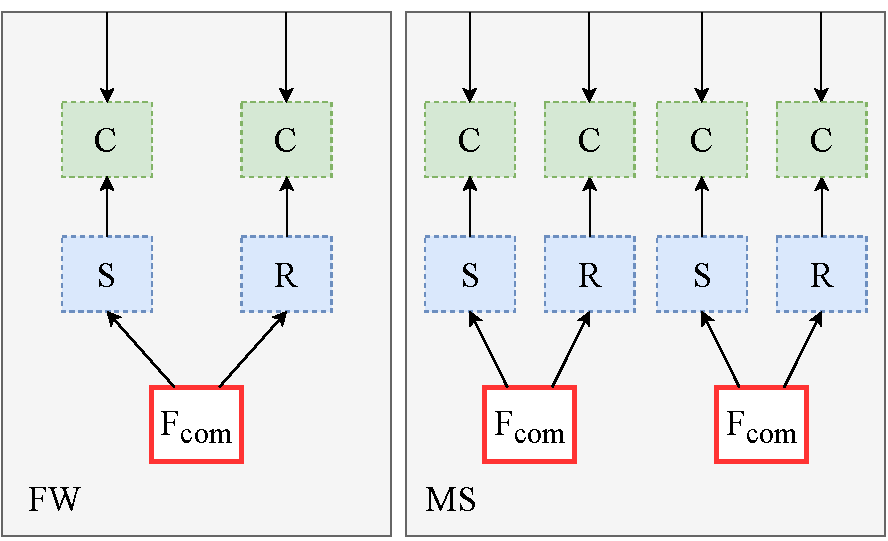
\includegraphics[scale=0.5]{figures/multisession.pdf}
%\caption{The multisession extension of \Fcom (right) with only two instances, creates the same processes $S$ and $R$ (offering the session typed channel to \Fcom) for every created instance. A communicator per session buffers messages for the $S$ and $R$ processes to consume and forward along their session-typed channel to \Fcom.}
%\label{fig:multisession}
%\end{figure}

%As a generic construction provided by NomosUC, the multisession operator requires some code generation but only to accept an arbitrary number of virtual token types if the underlying \F simulators other processes. 
%Furthermore, similar to the functionality wrapper, the multisession operator constructs the processes around \F in the same way and spawns them on-demand.
%The process definition for $!\F_\msf{com}$ is shown in Figure \ref{lst:bangf} accepting two token types: the real token type $K$ and the virtual token type $K_1$ for instances of $\F_\msf{com}$.
%
%\begin{figure}
%\begin{lstlisting}[basicstyle=\footnotesize\BeraMonottFamily, frame=single, mathescape]
%$\tb{proc}$ bangF[K,K1][p2f,...] :
%  (k: $\tgr{Int}$), (rng: [Bit]), (sid: session[a]), 
%  ($\$$p: P2MS[p2f][f2p]) |- ($\$$ch: 1) =
%\end{lstlisting}
%\caption{The type definition for the multisession operator for functionalities and the correspond message type and import parameters. The operator for protocol parties is identical in code but differens in that the parameters to the \texttt{P2MS} type are for \texttt{Z2P} interaction.}
%\label{lst:bangf}
%\end{figure}

\begin{theorem}[PPT !]\label{thm:bangppt}
If a functionality $\F$ is well-resource-typed, then it's multisession extension $!\F$ is well-resource-typed.
\end{theorem}

We examine this theorem in greater detail in the appendix. 
At a high-level it is obvious that such a construction, activated polynomially many times, is well-resource-typed as long as the underlying functionality/protocol is well-resource-typed.
%\begin{proof}
%A \textit{well-resource-typed} \F guarantees a polynomial $T_{\F}$ bounding its execution.
%In the worse-case, the multisession operator must spawn a new instance of $\F$ an every activation. 
%Let $N_{\F}$ denote the total number of instances (and, hence, number of activations) of $\F$ created by the operator.
%Note that $N_{\F}$ is polynomial in the security parameter $k$ for all well-typed environments, protocols, and adversary.
%Therefore, there always exists a bounding polynomial to bound a polynomial number of simulated instances of \F.
%The polynomial can be given as:
%$$ P_{!\F}(n) = N_{\F} P_{\F}(n) + \mathcal{O}(N_{\F}) $$
%where the $\mathcal{O}(N_{\F})$ is due to the overhead of maintaining and accessing the set of all instances.
%
%Similarly, \F being \textit{well-resource-typed} ensures a valid token context for all processes it may simulate. 
%Therefore, it is clear that there exists a global connecting poltnomial $f$ that ensures a valid token context for $!\F$.
%\end{proof}


%\begin{figure}
%\begin{lstlisting}[basicstyle=\small\BeraMonottFamily, mathescape, frame=single]
%$\yo{type}$ p2bFmsg[a] = P2bF of ssid ^ a ;
%$\yo{type}$ p2bbFmsg[a] = P2bbF of ssid ^ ssid ^ a ;
%$\tg{(* z2p : comm[z2pmsg[p2bbf[a]]] *)}$
%$\tg{(* p2f : comm[p2fmsg[P2bf[a]]] *)}$
%pid = recv $\$$z2p ;
%m = recv $\$$z2p ;
%case m (
%  P2bbF(ssid1, ssid2, m) =>
%    send $\$$p2f P2bF(ssid1 + ssid2, m) ;
%)
%\end{lstlisting}
%\caption{The \textit{squash protocol} accepts a message intended intended for $!!\F$ of type \inline{P2MS[p2ms[a]][ms2p[b]]}, i.e. of the form $(\msf{ssid}_1, (\msf{ssid}_1, msg))$.
%It ``flattens'' it into a single $\msf{ssid}_3 = \msf{ssid}_1 + \msf{ssid}_2$ that can be passed to $!\F$. The result is the same number of instances of \F but behind only a single $!$ operator.}
%\label{fig:squash}
%\end{figure}

\begin{proof} (Theorem~\ref{thm:squash})
On examination the \msf{squash} theorem does constant work per activation and concantenates two \inline{ssid}s into one for messages going to the functionality and does the inverse for messages incoming from the functionality.
We provide more detail for a proof of Theorem~\ref{thm:squash} in the Appendix, however, it is clear to see that the this theorem holds with a trivial simulator.
%First we describe the \msf{squash} protocol where $!!\F$ are nested $!$ operators.
%The protocol accepts messages intended for $!!\F$ of type \inline{P2MS[p2ms[a]][ms2p[b]]}, i.e. of the form $(\msf{ssid}_1, (\msf{ssid}_2, msg))$, and ``flattens'' them into a single message of type $\inline{P2MS[a][b]}$, i.e. of the form $(\msf{ssid}_3, msg)$.
%
%In $(\idealP, !!\F)$, \idealP~expects to receive messages of the form $(\msf{ssid}_1, (\msf{ssid}_2, m))$ where $\msf{ssid_2}$ is a sub-session of $\F$ (i.e. instance) inside some $!\F$ with sub-session id $\msf{ssid}_1$ inside of $!!\F$ (the message accesses functionality $\F[\msf{ssid}_1][\msf{ssid}_2]$).
%The \msf{squash} protocol flattens the indexing of instances of \F and combines session ids $\msf{ssid}_1$ and $\msf{ssid}_2$ into a single \msf{ssid}: $\msf{ssid}_3 := \msf{ssid}_1 \cdot \msf{ssid}_2$.
%If follows intuitively that the view for the environment remains the same. 
%
%We construct a simulator such that:
%\[
%\msf{execUC} \, \Z \, \idealP \, !!\F \, \SIM{\msf{squash}} \approx \msf{execUC} \, \Z \, \msf{squash} \, !\F \DA 
%\]
%The simulator is very simple. 
%Inputs to/from parties/\Z for a corrupt party is forwarded unmodified.
%Input intended for $!\F$ of the form $(\msf{ssid}_1 \cdot \msf{ssid}_2, msg)$ is sent as $(\msf{ssid}_1, (\msf{ssid}_2, msg))$ to $!!\F$. 
%Output from $!!\F$ is modified inversely and sent to \Z.
%
%The proposed simulator is trivially analyzed to be \textit{well-resource-typed}.
%It performs constant work per activation and does ``real'' simulation other than message modification to/from $!!\F$.
\end{proof}

\subsection{UC Composition}
Finally, we can conlude with full composition in Theorem~\ref{thm:compose}.
The proof follows directly from Theorems~\ref{thm:singlecomp} and \ref{thm:squash}.

\begin{proof}
By Theorem~\ref{thm:singlecomp} we can construct a simulator \SIM{1} for $!!\F_1 \xrightarrow{\rho \, \circ \, !\pi} \F_3$.
Theorem~\ref{thm:squash} then allows us to ``squash'' $!!\F_1$ and construct a simulator using \SIM{1} for $!\F_1 \xrightarrow{\rho \, \circ \, !\pi \, \circ \, \msf{squash}} \F_3$
\end{proof}

\subsection{Design Discussion}
One of the core research questions that this work aims to study session types applied to the UC framework. 
In this section, we discuss how resource-aware session types impact the design of functionalities in NomosUC as well as which are implementable.
We use the two-way authenticated channel functionality \Fauth to througout this discussion.

In plain session types, communication between two parties $P_s$ and $P_r$ occurs over a single duplex channel.
In UC the role of the adversary as a message scheduler in \Fauth, the most common network channel model, means a more complicated functionaty involving $P_s$, $P_r$, \F, and \A. 
The simplest, and most common approach, to \Fauth is the following communication pattern: a party $P_s$ sends a message to \Fauth, \Fauth sends the message to \A and waits for \A to say \inline{OK} before delivering the message to $P_r$.
Since both parties can send a message and receive a message, it is unclear which process, \Fauth or $P$, will be active along that channel at any given time.
Session types require this information to be statically known when two processes are communicating over a single channel--making this communication pattern unexpressable over a single channel.

There a few ways to overcome this constraint. 
In general, even though the UC framework places few restructions of communication patterns, most functionalities stick to a few.
\Fauth, for example, can take a few forms:
\begin{enumerate}
\item (presented above) Receiver and adverasry are activated directly: \Fauth waits for \A to tell it to deliver the message.
\item \Fauth ``polling'' approach: messages from $P_s$ are buffered for both \A and $P_r$. \A and $P_r$ must ask \Fauth for new messages. This is a more invonconvenient method, but can be useful for novel functionality designs that need a channel.
\item ``polling'' but receiver is activated: the message is stored in a buffer for \A, and \A's deliver message directly sends it to $P_r$.
\end{enumerate}
The simplest way to implement \Fauth in NomosUC is ``polling'' approach. As far as we know, we can systematically tranform any UC functionality into one that uses ``polling''. 
The consequences are that polling is inconvenient from a programming point of view because \Z needs to continuously activate parties to ask for new messages.
Hope is not lost though, because it turns out our type system can express functionalities in all three of the ways listed above. 
The first, and most natural, approach only requires splitting communicating between $P$ and \Fauth into two unidirectional channels
Such an extension to NomosUC trivially modifies the \partywrapper to handle two channels instead of one, and the types of the channels can be succintly expressed as: 
\begin{center}
\parbox{0cm}{
\begin{tabbing}
$\m{sending}[a] = \textcolor{red}{\getpot^n} \ichoice{\mb{sendmsg}: \m{a} \tensor \m{sendmsg}}$ \\
$\m{receive}[a] = \textcolor{red}{\getpot^m} \echoice{\mb{recv}: \m{a} \tensor \m{receive}}$ \\
$\m{adv}[a] = \echoice{\mb{leakmsg}: a \tensor \ichoice{ \mb{ok}: \m{leakmsg}}}$
\end{tabbing}}
\end{center}
The first to correspond to the channels for sending from $P$ to \Fauth and the second in the opposite direction. The third is the adversary's channel at \Fauth.

A notable part of our contruction is the machinery created around the protocol parties and functionality that intemediate their communication with communicators and functionally-typed messages.
Recall that such compromises are required in order to allow a \emph{dynamic} number of parties in UC.
The session type of the shared channel of a communicator only allows for a fixed amount of import to be sent over it with every messages. 
Protocols and functionalities that send different amounts of import depending on the message, say $i_1,...,i_n$, must now send $\m{max}(\{i_j\})$ import with every messages.
For existing UC definitions this appears to be an issue of ensuring a machine has \emph{enough} import, however, we can systematically map any UC import definition to one that works in NomosUC~\footnote{The problem can be reduced to ensuring enough ``latent'' import needed to compute, and, because we aren't concerned here with \emph{tight} computational bounds the problem is quite easy to solve. We discuss in greater detail in the appendix.}.



%\caption{The \msf{execUC} function used for the two-party commitment example used througout this paper. Recall, the \msf{execUC} is customized insofar as it takes in some number of virtual token types (here, $K_1$) to enable machines that simulate other machines. In the commitment example, there is no such simulation happening at the protocol or functionality level, therefore only the real token type $K_1$ is used here. The funtion spawns all the necessary ITMs in the UC execution: the environment, the protocol wrapper, the functionalty (wrapped), and the adversary. Each is parameterized with the security parameter $k$ and a random bit sequence $\msf{rng} \in \{0,1\}^{poly(k)}$.
%At the end, the environment is started and it returns a bit $b$ which is its guess for which world it is in. The full code can be found in the Appendix.}
%\label{lst:execuc}
%\end{figure*}

%We separate NomosUC into two modules: generic code and protocol-specific code. 
%Therefore, the \inline{execUC} refers to user specified code through the \inline{PS} module which defines \inline{PS.env} for \Z, \inline{PS.func} for the functionality, \inline{PS.prot} for the protocol, and \inline{PS.adv} for the adversary.
Communication between all of the major processes in the UC execution (\Z, \A, \partywrapper, and \fwrapper) is done through communicators introduced in Section~\ref{sec:nomosuc}.
Communicators are restricted to only sending functionally types messages in NomosUC, and we give generic types, below, to all such messages.
\todo{Is this important to even have here? seems a useless implementation detail.}
\begin{lstlisting}[basicstyle=\footnotesize\BeraMonottFamily, frame=single, mathescape]
$\Type$ p2zmsg[a] = P2Z of pid ^ a ;
$\Type$ p2fmsg[a] = P2F of pid ^ a ;
$\Type$ f2pmsg[a] = F2P of pid ^ a ;
\end{lstlisting}

\paragraph{The Environment}
The environment is the first machine that \inline{execUC} spawns and receives from it the session id and list of corrupted parties for this execution.
Its offered channel type \inline{EtoZ} specifies the interaction between \inline{execUC} and \Z:
\begin{lstlisting}[basicstyle=\footnotesize\BeraMonottFamily, mathescape, frame=single]
$\Type$ EtoZ[a] = +{init: a ^ list[pid] -> exec} 
$\Type$ exec = &{start : output_bit} ;
$\Type$ output_bit = +{bit: Bit -> 1} ;

$\tb{proc}$ PS.env[K][z2p,...]{p2zn,...} : 
  (k: $\tgr{int}$), (r: [Bit]), (#ztop: comm[z2pmsg[z2p]]{z2pn}), 
  (#ptoz: comm[p2zmsg[p2z]]{p2zn})...  |- ($\$$z : EtoZ) $\tg{(* <- offered channel *)}$
\end{lstlisting}
The environment also accepts communicators, as parameters, for communication with the protocol parties and the adversaries (in both directions), and offer a channel \inline{$\$$z} of type \inline{EtoZ}.
The type (above) states \Z provides an \emph{sid} of some user-defined type \inline{a} and a list of the \emph{pid}s of corrupted parties. 
Finally, \inline{execUC} instructs it to \inline{start} (\emph{external choice}) and return a bit $b$ as its guess for which world it is in.

%The \inline{\{z2pn\}}, for example, specifies the amount of import that must be sent by \Z with every message to a protocol party.
%The rest of the processes---the adversary, protocol wrapper, and functionality--are declared in the same way except the type parameters they expect are different: the protocol wrapper would of course accept type parameters for communication between it and \F, \A, and \Z.
%Finally the type of the offered channel \inline{$\$$z} is the same for all environments and communicates the \inline{sid} and set of corrupt parties chosen by \Z to \inline{execUC}.
%The \inline{sid} and corrupt list are parameters to the rest of the processes that \inline{execUC} spawns. 

%The communicators created by \inline{execUC} always use the same parametric types. 
%For example, for communication with the protocol, the types look like:
%\begin{lstlisting}[basicstyle=\small\BeraMonottFamily, frame=single, mathescape]
%$\Type$ p2zmsg[a] = P2Z of pid ^ a ;
%$\Type$ p2fmsg[a] = P2F of pid ^ a ;
%$\Type$ f2pmsg[a] = F2P of pid ^ a ;
%\end{lstlisting}
%Subsequently, the channel from \Z to the protocol wrapper will be typed as: \inline{comm[z2pmsg[z2p]]\{z2pn\}} where \inline{z2p} is a protocol-specific message type.
%The protocol \inline{PS.prot} is not spawned by \inline{execUC}. Instead the process spawns the protocol wrapper (described below) which spawns parties with that run the code \inline{PS.prot}.
%When in the ideal world, the protocol is given as the ideal protocol: one where the protocol wrapper converts the message from type \inline{z2pmsg[a]} to type \inline{p2fmsg[a]} but forwards the contents unaltered.
%The protocol wrapper and functionality wrapper manage spawning the instance(s) of the functionality and protocol parties.
%Similarly, an environment \msf{PS.env} and adversary \msf{PS.adv} must be defined as well.
%The message types exchanged between the processes are provided directly to \msf{execUC} as type parameters of the form \msf{p2f}, \msf{f2p}, and so on. 
%The first thing \inline{execUC} does is create the communicators and the corresponding channels for the main processes of the execution. 

%A consequence of using communicators is that in the UC setting they require at least 1 unit of import, beacuse they are activated a potentially polynomial number of times. 
%Therefore, all communicators in NomosUC receive some amount of import $n$ and send out only $n-1$. 
%The user-specified protocol, environment, functionality, and adverasary must account for this to ensure suffiient import is given to them.
%\begin{lstlisting}[basicstyle=\small\BeraMonottFamily, frame=single, mathescape]
%#ptoz <- communicator_init[K][p2zmsg[p2z]]
%           {p2zn+1} ;
%#ztop <- communicator_init[K][z2pmsg[z2p]]
%           {z2pn+1} ;
%...
%\end{lstlisting}
%This is strictly a design decision where user-defined protocols only specify import token requirements for the protocol not taking communicators into account. 
%The processes that they write, though, must conform to this standard and send an import token in addition to the amount they need.
%An alternate design would be that all import type parameters take the additional import token into account and communicators send one less than they receive.
%The drawback of the latter approach is that that when communicating with a process directly rather than through communicators (say, when simulating), you're sending one extra token for no reason.

%Next, the environment \msf{PS.env} is spawned, \inline{execUC} receives the \inline{sid} and corrupt list from \Z, and, finally, the remainder of the processes are spawned with these inputs. 
%Finally, the environment executes its own code when activated by \msf{\$z.start}, given the initial amoutn of import \inline{n}, and returns a bit through \inline{$\$$z.output_bit} which is its guess whether it's in the real or ideal world:
%\begin{lstlisting}[basicstyle=\small\BeraMonottFamily, frame=single, mathescape]
%$\$$z.start
%$\tb{pay}$ $\$$z {n}
%$\$$d <- $\$$z
%\end{lstlisting}

\subsection{The \partywrapper}
NomosUC departs slightly from the standard UC framework by using a \partywrapper to encapsulate all protocol parties and run them internally.
Rather than passing protocol party channels as parameters to \Z or \A (supporting a static set of parties), the \partywrapper provides a single endpoint for all messages to parties.
Similarly we adapt a \fwrapper to function like the \partywrapper but on functionalities. The main pupose of this wrapper and the \partywrapper is to intermediate communication between the session types the functionality uses and the functionally typed messages exchanges through communicators.

Like \iexecuc, we genrate the \partywrapper based on the protocol or functionality being executed. 
Converting between functional and session-typed messages is an easy task to automate and we push that onto code generation rather than requiring a user to produce it.
The extra processes generated within the \partywrapper are shown in Fiure~\ref{fig:blankpartywrapper}.
%In a nutshell, the wrapper accepts messages from a communicator, say from \Z, demultiplexes it, converts its type to one over a session-typed channel and conveys it to the necessary protocol party.

Following along with Figure~\ref{fig:blankpartywrapper}, the generated processes \inline{C} are use to de-multiplex messages based on the \inline{pid} of the receipient, and the \inline{z2p} and \inline{p2f} processes convert messages between the session typed channels and the functional messages that are received.
The arrow notation in Figure~\ref{fig:blankpartywrapper} indicates the $\m{prodiver} \leftarrow \m{client}$ relationship for each channel and provides their types.

We elaborate on the processes \inline{z2p}. For the commitment protocol the messages received by the \partywrapper are type as 
\begin{lstlisting}[basicstyle=\footnotesize\BeraMonottFamily, mathescape]
$\yo{type}$ comp2f = Commit of Bit | Open ;
$\yo{type}$ comf2p = Committed | Open of Bit ;
\end{lstlisting}
and the \inline{z2p} process intercepts them and communicates to the party over a channel typed with the \Fcom session types in Section~\ref{sec:nomosuc}.
For example when \Z gives the command to commit to a bit, \inline{z2p} does the following:
\begin{lstlisting}[basicstyle=\footnotesize\BeraMonottFamily, frame=single, mathescape]
case msg (
  Commit(b) =>
    $\$$z2p.commit ;
    $\tb{send}$ $\$$z2p b ;
    $\tb{pay}$ {z2pn} $\$$z2p ;
\end{lstlisting}
where \inline{$\$$z2p} is the session-typed channel to the committer.
The \inline{f2p} processes does the same for communication between the parties and the functionality.

Virtualizing the protoocl parties means that the wrapper and the parties it runs are, effectively, using the same import and potential.
We reason that the \partywrapper and protocol parties it runs will always have enough import by noticing that the \partywrapper does constant work on each activation.
Therefore, if protocol parties intend to hold on to import, there is always a suficient polynomial to allow both the wrapper and the party to perform potentially polynomial computation.
\todo{Reword this to make it crisper}.

%Folling along with Figure~\ref{fig:blankpartywrapper}, the generatd processes \inline{z2p} and \inline{f2p} communicate with the party over a session-typed channel and perform the message type conversion mentioned above based on a simple message type mapping provided by the user.
%The \inline{z2p} process offers a linear channel to the party with the correct session type with \Z. 
%The wrapper reads messages from \Z, demultiplexes them based on \inline{pid} and puts them in the appropriate virtual communcator (the green box labeled \inline{C}) for the \inline{z2p} processes to read from, convert, and send to the party.
%The protocol party offers a linear channel of its type with \F, and \inline{p2f} converts this to a functional type. \inline{p2f} offers the same type as a communciator to the wrapper which reads the message and sends it to \F. 
%Figure~\ref{fig:blankpartywrapper} indicates the type of the offered channel for all the relevant processes within the wrapper. 

%In order to use session types, the each protocol party is internally connected to two processes \inline{z2p} and \inline{f2p} over with session-typed channels for their communication with \Z and \F, respectively.
%\inline{z2p} is connected to party-specific virtual communicators so that \inline{z2p} and \inline{f2p} can read/send messages from. It can not read/write directly to/from the actual communicators connecting the protocol wrapper because, being simulations inside the protocol wrapper, they do not use the same token type.
%In the case of the ideal world with \Fcom, the both of the sender's ($\pi_1$) channel with \inline{z2p} channels with \inline{z2p} and \inline{f2p} are typed as \inline{sender}, and the protocol party itself ($\pi_1$) just fowards messages from one channel to the other.

%The processes \inline{Z2p} and \inline{f2p} are generated for each party based on their session-type, and they convert between them and functional messages for incoming/outgoing communcation with \Z, \F, or \A. 
%For example in the commitment example, where the functional message type is given by: 
%\begin{lstlisting}[basicstyle=\footnotesize\BeraMonottFamily, mathescape]
%$\yo{type}$ comp2f = Commit of Bit | Open ;
%$\yo{type}$ comf2p = Committed | Open of Bit ;
%\end{lstlisting}
%the \inline{z2p} process does something like this for the sender (where \inline{msg} is received from its virtual communicator):
%\begin{lstlisting}[basicstyle=\footnotesize\BeraMonottFamily, frame=single, mathescape]
%case msg (
%  Commit(b) =>
%    $\$$z2p.commit ;
%    $\tb{send}$ $\$$z2p b ;
%    $\tb{pay}$ {z2pn} $\$$z2p ;
%\end{lstlisting}
%It sends a commit message over the linear channel with the sender, and pays the necessary amount of (virtual) import tokens with the message.
%When \Z, \A, or \F send a message to a party that doesn't exist, the \partywrapper creates the new party's \inline{z2p}/\inline{f2p} processes and an instance of the party itself, and it connects them together in the same way shown. 
%We do something similar for functionalities, in Appefix~\ref{app:fwrapper}

\begin{figure}
\centering
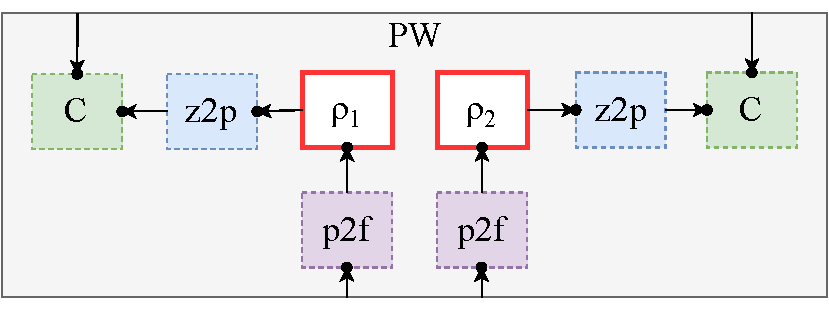
\includegraphics[scale=0.5]{figures/blankpartywrapper2.pdf}
\caption{The internals of the protocol wrapper with two parties. The arrows indicates the client/provider relationship between each pair: provider $\rightarrow$ client. The wrapper creates \texttt{z2p} to offer a channel and convert from gunctional to message type---the \texttt{p2f} do the same. A communicator is used because \texttt{z2p} cannot send message to real one with differing token type. The types of the processes offered are (color): \tgr{comm[z2pmsg[comp2f]]}, \tb{sender}, \tr{party[Int]}, \tp{comm[p2fmsg[rop2f]]}. }
%The processes \texttt{z2p} offer linear channels to their respective protocol parties that are typed according to that party's protocol, and they receive messages from virtual communicators that hold messages specific to one \texttt{pid}. The protocol code for $\pi_1$ and $\pi_2$ are user-specified and offer a channel to the \texttt{p2f} process according to their protocol with the functionality. The \texttt{p2f}s convert outgoing messages to, and incoming messages from, functional message types to be sent to/from the functionality. The protocol wrapper gives messages to the virtual communicators and receives messages from \texttt{p2f}s.}
\label{fig:blankpartywrapper}
\vspace{-1.5em}
\end{figure}

%For the commitment example, if $\pi_1$ and $\pi_2$ ran the commitment protocol, \inline{z2p} would offer a channel of type \inline{sender} and \inline{receiver} to $\pi_1$ and $\pi_2$, respectively, and it converts between the functional messages for the commitment protocol and the session typed ones. 
%In the ideal world, the $\pi_1$ and $\pi_2$ run a dummy protocol where their offered channels are simply forwarded to their \inline{z2p} channels, i.e. the \inline{z2p} and \inline{f2p} channels have the same type: \inline{sender} and \inline{receiver}, respectively.
%In the style of Nomos, the protocol wrapper:
%\begin{itemize}
%	\item Attempts to read messages incoming from \Z, \A, or \F and forward them to the appropriate process depending on \inline{pid}.
%	\item Read from the internal communicators or the \inline{p2f} processes for outcoing messages.
%\end{itemize}
%For reference the functional messages typed for the commitment protocol are:

%Recall the session types for the sender and receiver, with \Fcom, introduced in Section \ref{subsec:idealcommitment}.
%%\begin{gather}
%%	\mi{stype} \; \m{sender} = \ichoice{\mb{commit} : \m{bit} \product \m{scommitted}} \\
%%	\mi{stype} \; \m{scommitted} = \ichoice{\mb{open} : 1} \\
%%	\mi{stype} \; \m{receiver} = \echoice{\mb{commit} : \m{rcommitted}} \\
%%	\mi{stype} \; \m{rcommitted} = \echoice{\mb{open} : \m{bit} \arrow \one}
%%\end{gather}
%At the beginning there are no parties. When the \A or \Z write to a party with some pid $p$ the protocol wrapper creates $p$ if it does not exist.
%It creates and stores the session-typed channels or all of the parties in channels corresponding to their type and moves channels between them as the type evolves.
%For example for parties' channel with \Z the protocol wrapper generates the following lists:
%\begin{gather}
%	\m{R1L1}[\m{sender}] \\
%	\m{R1L2}[\m{scommitted}] \\
%	\m{R2L1}[\m{receiver}] \\
%	\m{R2L2}[\m{rcommitted}] 
%\end{gather}
%At the beginning of the protocol, the committer's \msf{z2p} channel would be in \inline{R1L1} and the receiver's is in \inline{R2L1}.
%The channel's connection the protocol wrapper to the rest are still functionally typed. It's channel \inline{p2f} will still be typed \inline{#ptof: comm[p2fmsg[comp2f]]} where \inline{comp2f} is:
%Succinctly, the protocol wrapper functions as follows:
%\begin{itemize}
%\item When the protocol wrapper receives a message for some \msf{pid}, if the party doesn't exist the protocol wrapper creates all the party's channel parameterized by the correct session types (the role of the party is determined by the incoming message). The channels are stored and outgoing channels are waiting to be read from.
%\item The message sent to the party with the session type is determined by the functional type. The wrapper creates a session-typed message and forwards the contents of the message to the party.
%Despite accepting functionally typed messages, the protocol wrapper uses session types in this way to allow the type checker to catch invalid and out of order environments, adversaries and functionalities. 
%For example, in the commitment protocol when the committer tries to commit a bit in \Fcom like this:
%\begin{lstlisting}[basicstyle=\small\BeraMonottFamily, frame=single, mathescape]
%$\$$p2f.commit 
%$\tb{send}$ $\$$p2f b
%$\tb{pay}$ {p2fn} $\$$p2f
%\end{lstlisting}
%\begin{lstlisting}[basicstyle=\small\BeraMonottFamily, frame=single, mathescape]
%$\$$p2f.SEND 
%$\tb{send}$ $\$$p2f pid 
%$\tb{send}$ $\$$p2f Commit(b)
%$\tb{pay}$ {p2fn} $\$$p2f
%\end{lstlisting}
%The party wrapper intercepts and converts it to a functionally typed message:
%\item For outgoing messages, the protocol wrapper does a similar conversion where it reads the sesion typed channel output by the party and converts its message to the appropriate functional message type.
%\end{itemize}

%\paragraph{Functionality Wrapper}
%The \fwrapper adopts a similar approach to the \partywrapper, except it only creates one instance of the underlying functionality.
%For the same reason as the \partywrapper, we use an \fwrapper to enable a dynamic set of parties.
%One caveat in supporting such functionalities, is that, so far, only functionalities whose type follows a specific form are allowed.
%In the random oracle type given below, notice that the type before and after a party interacts with it is the same: type $\m{party}[a]$.
%\begin{mathpar}
%\m{party}[a] = \textcolor{red}{\getpot^1} \ichoice{\mb{hash} : \m{pid} \arrow \m{int} \product \m{hashing}[a]} \\
%\m{hashing}[a] = \echoice{\mb{shash} : \m{pid} \arrow \m{int} \product \textcolor{red}{\paypot^0} \m{party}[a]} 
%\end{mathpar}
%A party queries a $\mb{hash}$ of an integer from \Fro and receives an integer as a response. The session type includes the \inline{pid}, which enables it to handle all parties over the same channel.
%
%An example of the internals of the \fwrapper are showing on the left-hand-side of Figure~\ref{fig:multisession}.
%Like the \inline{z2p} processes in the \partywrapper, \inline{S} and \inline{R} represent the sender and receiver in the commitment protocol, and they read from their virtual communicators and communicate with \Fcom over a session-typed channel.

%When a party invokes \Fro, the type it expects is \inline{party[a]}, and when it has received its hash the type is again back at \inline{party[a]}. 
%The wrapper handles such dynamic functionalities by channeling all party communication through one linear channel in the wrapper. 
%Therefore, \Fro reads on one channel and responds to the specific party with some \inline{pid}, and the protocol wrapper remains unchanged. 
%
%The constructions of the protocol wrapper and functionality wrapper enable users to write very simple ideal functionality and protocol code, as we will discuss in the next Section and in the Appedix.

%In the commitment example, \Fcom accepts two channels, one from each party, and two processes are created (call then \inline{p2f} for now) which offer channels of type \inline{sender} and \inline{receiver}, respectively. 
%The wrapper differs from the protocol wrapper for certain functionalities that accept a dynamic number of parties. 
%Continuing with our commitment example, the random oracle functionality, an idealized hash function, is used in the real world to realize \Fcom, and it allows a dynamic set of parties to inteact with it.
%Its session type with protocol parties is given below.
%The session type is special in that, for every interaction, the channels type always ends up back at \inline{party[a]} before any other party tries to use \Fro.
%NomosUC enables ideal functionalities whose types work like this by adding the \inline{pid} to the type, and having only one process in the functionality wrapper offering a channel of this type to \Fro.
%Unlike \Fcom where new communicator and \inline{p2f} process is created for each new party, messages from all parties pass through one such process.
%Additionally, moving the \inline{pid} into the session type means that the protocol wrapper can create arbitrarily many \inline{pid}s to communicate with \Fro.

\paragraph{The Adversary}
The adversary, much like the environment, is providing input to the protocol and functionalities.
As the UC framework is concerned with modular construction for protocols, and NomosUC with using session types to aid in suc construction, we do not give adversaries session types.
Therefore, they are not wrapper like protocols and functionalities, and communicate with all other processes directly through functional message types.

\subsection{Polynomial Bound}
The security of the UC framework relies on computational constraints on adversaries, and, generally, on what all ITMs can do.
It introduces the concept of import tokens as a new way to reason about ITMs being polynomial in the security parameter $k$. 
The import mechainsm as described in UC, and which we descrive in Section~\ref{sec:background}, ensures that a single ITM's execution is upper-bounded by some poynomial $T(n,k)$ where $T$ is a polynomial, $n$ is its net import token balance (received - sent), and $k$ is the security parameter.
Canetti et al. limit their discussion to parameterized systems where all machines do not do anything until they have received at least $k$ import.
We depart from this notion slightly and express ``interactive polynomial time'' by using a bounding polynomial in both import and $k$.
We do this for two reasons.
First, it remedies our exclusion of ``parameterized systems'' by easing the import requirements of cacnonical cryprograpic operations, such as a random oracle operation on $k$-bit strings that would otherwise require $k$ import. 
Second, we add $k$ to reflect a more natural notion of import and modularity in UC by allowing minimial import for constant-work one-shot processes like \Fcom which no longer need import just to handle $k$-bit strings.

In NomosUC, we build import into the type system to be able to reason about ITMs being locally polynomial time given some polynomial $T$.
Specifically, the system provides novel constructs to exchange import, generate potential from that import, and create virtual import for simulating other machines.
%Specifically, the type system can check whether a given polynomial bound in the import amount satisfies the potential generated/used by an open Nomos term.
The language additionally encodes the computational cost of each operation performed by an ITM, and statically guarantees that the execution cost of each ITM is locally polynomial in the net import it has over its entire execution. 
The locally polynomial invariant can be extended to claim that the entire UC execution of locally PPT ITMs is also PPT.

\begin{ddef}[PPT in $k$]\label{def:ppt}
A term $e(k,r)$ is \emph{well-resource-typed} and PPT if, given some amount of initial import $n$, there exists a polynomial $T(n,k)$ such that $\forall k, r, e(r,k) \{n\}$ terminates in at most $T(n,k)$ steps. 
\end{ddef}

%\begin{proof}
%The Nomos type system only type checks programs for which a satisfying assignment of polynomial $T$ is possible.
%Given an $n \in poly(k)$, all programs that type check must be \textit{well-resource-typed.}
%%The Nomos type system guarantees that a satisfying assignment of $n$ and $T$ will correctly type-check.
%%Therefore, given an initial amount of import $n(k) \in poly(k)$, the existence of some $T$ ensures that any process, regardless of its randomized execution according to the bit sequence $r$, $e$ is guarantees to be upper-bounded by $poly(k)$ satisfying the definition of probabilistic polynomial time in $k$.
%\end{proof}

%We demonstrate that our local PPT definition implies a PPT UC execution by adapting Proposition 7 from the UC framework to the NomosUC setting.
%Our sandboxing mechanism and \inline{withdrawTokens} procedure let us simulate the well-resource-typed ITMs, in the UC execution, within one ITM.
%We need only provide a suitable ``exchange rate function'' \GlobalF and a bounding polynomial $T$ on the single machine to conclude that it is well-resource-typed.
%If the initial import given to the system is $n$ then the single ITM generates $n$ virtual tokens, and simulates all inputs generated by the environment.
%Subsequently a sufficient bounding polynomial for this ITM is to the order of $O(n \times T')$ wher $T'$ is the largest polynomial among those bounding the simulated machines. The additional factor of $n$ exists to allow for routing/handling of messages between simulated machines.
%Clearly, this is not a tight bound but it will bound the entire UC execution, and our \inline{withdrawTokens} rules ensures that we are left with a valid token context.
%Therefore, the resulting UC execution, as a single ITM, is also well-resource-typed.

The soundness of our polytime notion comes down to showing that our UC experiment is PPT in only the security parameter $k$. 
The UC framework provides a simulation of a configuration of ITMs on a universal turing machine and proves that such a turing machine is also bounded by a polynomial $T$. 
Given the initial input of import tokens into the machine ($poly(k)$ amount of import), it can conclude that their import mechanism falls in line with the standard notion length-of-input polynomial time and satisfied their ``PPT in $k$'' definition. 
In NomosUC, we do not deal directly with ITMs, however, our type system allows us to judge whether a process, or collection of processes through the Preservation Theorem~\ref{thm:preservation}, is locally PPT given a particular polynomial. 
We use this judgement as a foundation and adapt Proposition 7 from UC~\cite{uc} to NomosUC, and show that our notion of locally PPT leads to a UC execution that is PPT in the security parameter $k$.

\todo{Define \F, \A, \Z, \m{PW}(\PI) as configurations that include the communicators to be used. Just need to create a standard for which direction communicator is part of which configuration.}
\begin{theorem} \label{thm:soundness}
Let \F, \A, \Z, and \m{PW}(\PI) be locally PPT configurations bounded by super additive polynomials $T_\F$, $T_\A$, $T_\Z$, $T_\PI$. Let \m{UC} be a configuration composed of a single process that runs \inline{execUC},. If \m{UC} receives $n \in poly(k)$ import initially, then the composed configuration $\m{UC} = \m{execUC} \; || \; \Z \; || \; \A \; || \; \m{PW}(\PI) \; || \; \F$ is PPT in $k$, where \m{PW} is the \partywrapper.
\end{theorem}

\begin{proof}
The resulting configuration \m{UC} has only one channel in it's context: the channel offered by \inline{execUC} of type \inline{Bit}. 
\inline{execUC}, therefore, is the intial process in the configuration and receives the intial import $n \in poly(k)$.

By the \m{compose} rule, the work done by the resulting configuration is strictly the sum of the work done by the composed configurations. 
The Preservation Theorem in conjunction with \m{compose} ensures type safety of \m{UC}, and allows us to concluce a sufficient bound on the total work done in \m{UC} by the polynomial $T'(n,k) = T_\A(n,k) + T_\Z(n,k) + T_\P(n,k) + T_\F(n,k) + O(1)$ where $n$ is the initial import into the system, and the addition $O(1)$ accounts for the constant bound on \inline{execUC}.
If we take the intial import $n$ to be polynomial in the security parameter $k$, we conclude that \m{UC} is PPT in $k$.
\end{proof}

\paragraph{Sending/Receiving Import}
Our construction of the UC experiment requires communicators (introduced in Section~\ref{sec:nomosuc}) to intermediate communication between the \Z, \A, \F, and \m{PW}(\PI).
Their use adds import requirements to the experiment that are not captures by just the types of \F, \A, and \PI. 
It results from them being activates a potentially polynomial number of times. Therefore, the communicator's type, introduced in Section~\ref{sec:nomosuc} defines the, reflects this computation by
retaining one of the import tokens that is sent accross it. 
Given that our functionalities are parameteric in the amount of import they send/receive (so as to not restriction wat protocols can realize them), the user must take into account the number of import taken by communicators.
In our commitment example, the messages from \Z that uses the most import in the real world is the sending the \inline{open} message to the committer. This activationa results in 5 communicators being activated and so five more import than the protocol already requires. As long as the ideal functionality is parameterized to accept the same amount of import, indistinguishability still holds. \todo{This belongs somewhere else}.

%Our construction of the \partywrapper and \fwrapper rely on sending functional messages between them through a shared communicator.
%The same holds true between the adversary and the two wrappers, and also holds true between the environment and the \partywrapper.
%When any of these parties is sending import to each other, they must always send the maximum import of any message that can be exchanged with each other.
%For example if parties $p_1$ and $p_2$ send $n_1$ and $n_2$ import to the functionality, then the communicator between the \partywrapper and \fwrapper will be typed to expect $max(n_1, n_2)+1$ import on every message from the \partywrapper and vice versa for messages from \fwrapper to \partywrapper. 
%Recall from Section~\ref{sec:nomosuc} that the $+1$ is required to give the communicator at least one unit of import.
%Similarly, \Z will send the maximum of the imports required by $p_1$ and $p_2$ plus two additional import for communicators.
%In total, for any activation by \A or \Z there can be up to three communicators activated in the execution. 

%An simple example where that illustrates the type system's capabilities is the authenticated append/read functionality $\F_\msf{AppRd}$~\footnote{We provide the code for this functionality in the appendix for the simplified case of a single party.}.
%The functionality requires parties to provide 1 unit of import to append items to the list and 1 unit of import to read from the list, and the functionality generates potential proportional to the length of the list in order to traverse it.
%It is clear that the total work performed by $\F_\msf{AppRd}$ is bounded by a quadratic poynomail, and the NomosUC type system ensures that only bounding polynomials quadratic or larger successfully type check.
%\todo{something more to say here}

%\begin{definition}[PPT Term]\label{def:pptterm}
%A \textit{PPT term} is a \textit{well-typed} term $e(k, r)$ that is \textit{closed} except for security parameter $k$, random bit sequence $r$.
%\end{definition}
%
%We first-define terms that are well-typed in the traditional session-types-sense in Definition~\ref{def:pptterm}, i.e. without any resource constraints~\cite{caires2010session}.
%Such terms are closed except for the security parameter $k$ and some uniformly random bit sequence $r$. 

%However, we also want to reason about terms that are well-typed when connected to another Nomos terms.

\subsection{Emulation}
Emulation underpins the UC security definition, and reasons about indistinguishability between two protocols over all adversaries against it and a simulator for all environments.
In NomosUC, we must be more careful to only consider protocols and adverasaries whose types (both message and import) match over the channels they share. 
Therefore, we introduce the term \textit{well-matched} to mean a PPT term $e$ is well-typed when connected to another term $e'$.
Simply put, we want to capture terms $e$ and $e'$ that can be connected over the channels the share given their type.
The resulting terms in Definition~\ref{def:wellmatched} are partionall closed after connection: the terms may only be connected on some subset of their channels.
%Simply put, the channels that $e$ and $e'$ share are of the same type. 
%Specifically, we want to exclude processes that logically share a channel, say the channel from \inline{p} to \inline{f}, but send (their types message types don't match).
%This new definition becomes important when we discuss UC emulation below as we want to reason about environments that are \textit{well-matched} for a protocol $\pi$ or a specific adversary \A.

\begin{ddef}[Well-Matched]\label{def:wellmatched}
\begin{mathpar}
\footnotesize
\inferrule*[right=Well-matched]
{\Tokens_1, K \semi \Delta_1 \vdash e :: \Delta_1' \semi 
\Tokens_2, K \semi \Delta_2 \vdash e' :: \Delta_2' \\ \\
 S \equiv \Delta_1 \bigcap \Delta_2 \neq \emptyset}
%{\Delta_1 \leftrightarrow \Delta_2}
{\Delta_1 \equiv_{S} \Delta_2 \semi e \leftrightarrow e'} 
\end{mathpar}
\end{ddef}

In the UC security definition, we say that a protocol $\pi$ posesses the same security properties as another protocol $\phi$ if no environment can distinguish between them for any adversary.
In most cases we compare a real protocol $\pi$ with an idealized protocol $(\idealP, \F)$ which is actually just an ideal functionality with dummy parties.
The ideal functionality is known to achieve the desired security processes because it acts like a simple, trusted third party.
%They are much simpler than protocols because they don't require any special code to handle mutually distrustful other processes, and they perform the given computation on behald of the ideal world parties.

Given the random choices ITMs in UC can make, it is clear that the outputs of \inline{execUC} produces and ensemble of distributions over all possible random bitstrings and security parameters.
Emulation, then, is about the ensembles created by two UC environments being computationally indistinguishable from each other.
We define indistinguishabiliy between ensembles in a standard way using \textit{statistical distance} in Definition~\ref{def:distance}.

\begin{definition}[Indisinguishability]\label{def:distance}
Two ensembles $\mathcal{D}_{1,k}, \mathcal{D}_{2,k}$ are indistinguishable, $\mathcal{D}_{1,k} \sim \mathcal{D}_{2,k}$, if their statistical distance is at most $negl(k), \forall k$.
\end{definition}

%\paragraph{Validity}
%For the remainder of this section we refer to \emph{valid} adversaries and simulators given a particular protocol, functionality, or environment.
%We refer to adversaries that type-check when connected to \Z, \F, or $\Pi$ by \inline{execUC}, and that are \emph{well-matched} as defined above. 
%Indisintiguishability between two protocols is defined as follows (we shorten the communicator type \msf{comm} to \msf{c}):

UC emulation combines the UC exeution with indistinguishability resuting in the following NomosUC emulation definition.
\begin{definition}[Emulation]\label{def:emulation}
Given two protocols $(\pi, \F_1), (\phi, \F_2)$ that are well-resource-typed then if $\forall \A$ well-matched with $(\pi, \F_1)$, $\exists \Sim$ s.t. $\forall \Z$ well-matched with \A and $(\pi, \F_1)$: \Sim is well-matched with $(\phi, \F_2)$, \Z is well-matched with $(\phi, \Sim)$, and $\msf{execUC}(\pi, \F_1, \Z, \A) \approx \msf{execUC}(\phi, \F_2, \Z, \Sim)$:

\begin{mathpar}
\footnotesize
	\inferrule*[right=emulate]
	{
		%. \models \msf{execUC}[\Tokentypes][\alpha] :: \Delta[\Tokentypes][\alpha] \\ \\ 
		% Protocols that are well-matched with their functionalities
		%\pi \rightarrow \Delta_1' \semi \phi \rightarrow \Delta_2' \semi \\
		\pi : \Delta_1'[\Tokentypes][\mathrm{T}_{\pi}] \semi \phi : \Delta_2'[\Tokentypes][\mathrm{T}_{\phi}] \semi \\
		%\langle \pi \leftrightarrow \F_2 \rangle, \langle \phi \leftrightarrow \F_1 \rangle \\
		% Type of execUC[DELTA_pi] and execUC[DELTA_phi]
		\forall \A \, | \, \Delta_4[\Tokentypes][\mathrm{T}_{\A}] \vdash \A :: \Delta_4', \langle \A \leftrightarrow \pi \rangle\\
		%\Delta_1'[\Tokentypes][\mathrm{T}_{\pi}] \equiv_{\Z} \Delta_1\ 
		%\semi \Delta_2'[\Tokentypes][\mathrm{T}_{\phi}] \equiv_\Z \Delta_2 \\
		% For all A if exists well-typed A that is well-matched with real world
		%\forall \A, (\exists (\Delta_4, \Delta_4') | \Delta_4 \vdash \A :: \Delta_4', \langle \A \leftrightarrow \pi \rangle, \langle \A \leftrightarrow \F_1 \rangle \\
		%\forall \A | \Delta_4 \vdash \A :: \Delta_4', \langle \A \leftrightarrow \pi \rangle, \langle \A \leftrightarrow \F_1 \rangle \\
		% implies simulator that is well-matched for ideal world
		%\Rightarrow \exists (\Delta_3,\Delta_3') \, | \, \Delta_3 \vdash \Sim_\A :: \Delta_3', \\ % \langle \Sim_\A \leftrightarrow \phi \rangle, \langle \Sim_\A \leftrightarrow \F_2 \rangle \\
		\Rightarrow \exists \Delta_3[\Tokentypes][\mathrm{T}_{\Sim}] \vdash \Sim_\A :: \Delta_3', \langle \Sim_\A \leftrightarrow \phi \rangle \\ % \langle \Sim_\A \leftrightarrow \phi \rangle, \langle \Sim_\A \leftrightarrow \F_2 \rangle \\
		% for all Z they that's well-matched for the real world => Z is well-matched with S and ideal world
		%\forall \Z (\langle \Z \leftrightarrow \A \rangle, \langle \Z \leftrightarrow \pi \rangle \Rightarrow \langle \Z \leftrightarrow \Sim_\A \rangle, \langle \Z \leftrightarrow \phi \rangle \\
		% and emulation has to hold
		\Rightarrow \forall \Z \; \msf{execUC} \ \pi\ \Z\ \F_1\ \A \approx\ \msf{execUC} \ \phi\ \Z\ \F_2\ \Sim_\A
	}
	{
		% EMULATION DEFINITION
		\lambda \A . \Sim_\A \vdash (\pi, \F_1) \sim (\phi, \F_2) % \F_1 \xrightarrow{\pi} \F_2
		%\lambda \A . \Sim_\A \vdash (\pi, \F_1) \sim (\phi, \F_2)
	}
\end{mathpar}
\end{definition}
The emulation definition above is quite straightforward. It starts with defining the protocols in question and their type under the type parameters passed to \inline{execUC}.
It then states that for all adversaries that are well-matched with $\pi$ and $\F_1$, there exists a simulator such that the two executions are indistinguishable. 
The definition ensures that for emulation to hold, the constructed simulator must be well-matched everywhere \A is well-matched: for all environments \A is well-matched with the \Sim must also be well-matched with.

With this emuluation definition we complete our definition of UC-realization in Definition~\ref{def:realize}.
If a simulator exists such that emulation holds for $(\pi, \F_1) \sim (\idealP, \F_2)$ then we say that the protocol $\pi$ UC-realied the functionality $\F_2$ in the $\F_1$-hybrid world:
\[
	\F_1 \xrightarrow{\pi} \F_2
\]

\paragraph{Import for Functionalities}
The \Fcom example use throughough this work is realized by protocol that uses the random oracle. 
A natural notion of import should define \Fcom as requiring 0 import because it is one-shot and halts after doing constant amount of work.
\Fro on the other hand, requires at least 1 unit of import in order to be handle a potentially polynomial mumber of activations as well as reading/writing $k$-bit strings.
This poses a problem that the ideal world requires 0 import however, the real world requires at least 1 unit of import.
We resolve this dilemma by defining functionalities as parameteric in the amount of import they require.
Parametric functionalities do not restrict UC-realization to only those protocols that are as compitatiaonally ``efficient'' as the them. In cryptography, it is common for real protocols to be computationally intensive while the ideal functionality they are realizing is trivial, and we want to be able to express such emulation.
We modify the arrow notation, slightly, to capture that a functionality can realize itself while requiring more import, and use the notation $\F^m$ to denote a functionality parameterized to require $m$ import.
\[
	\F_1^m \xrightarrow{\idealP} \F_2^{n \geq m}
\]
For the remainder of this work we do not bother import annotations on functionalities and only concern ourselves with the minimum import they require because it is an implementation detail.

%When we talk about emulation, we particularly care about emulation with respect to an ideal protocol $\phi$ which is really just $(\idealP, \F)$ where \idealP is the protocol which forwards all messages to/from \Z and \F.
%We say the protocol $\pi$ (potentially with a hybrid functionality $\F_1$) UC-realizes an ideal functionality $\F_2$ if Definition~\ref{def:emulation} holds for $(\pi, \F_1)$ and  $\phi = (\idealP, \F_2)$

%\begin{definition}[UC-Realize]
%A protocol $\pi$ UC-realized an ideal functionality $\F_1$ if $(\pi, \F_2) \sim (\idealP, \F_1)$ for some $\F_2$.
%
%\begin{mathpar}
%\footnotesize
%\inferrule*[right=UC-Realize]
%{ (\pi, \F_1) \sim (\idealP, \F_2) }
%{ \F_1 \xrightarrow{\pi} \F_2 }
%\end{mathpar}
%\end{definition}

\subsection{Dummy Lemma} \label{sec:dummy}
The dummy lemma is a crucial result in UC that reduces the design space of simulators to just one: for the dummy adversary in the real world.
The Lemma states that if a simulator exists for the dummy adversary, called the dummy simulator \DS, then there it is easy to construct a simulator for any other adversary \A. 
The simulator constructed in this lemma uses virtual tokens to internally run \DS and \A.

The intuitiom behind this results rests in the fact that emulation must hold over $\forall \Z$ for a particular \A. 
Particularly, in the case of \DS and \DummyAdv, emulation holds for a \Z that may be running any other possible \A internally and passing it's output to \DS and \DummyAdv.
Therefore, moving \A out of the simulation and into the execution, as the real adversary and as providing input to \DS, should maintain emulation between the two worlds.

\begin{theorem}[Dummy Lemma]\label{thm:dummy}
If \ $\exists \DS$ s.t. $ \DA, \DS \vdash \F_2 \xrightarrow{\pi} \F_1$ then $\forall \A \ \exists \Sim_\A$ s.t. $\Sim_{\A} \vdash  \F_2 \xrightarrow{\pi} \F_1)$ 
\end{theorem}

We give the proof of this lemma in the appendix, however, we provide an intuition for understanding why it is true.
Simulation w.r.t the dummy simulator works for all environments, even those that could run any potential real-world adverasry internally. Such environments, pass input to the adversary, whose output is given to the dummy simulator. 
The constructed simulator captures the idea of moving the adversary from the environment into the the execution, and the constructed simulator runs the real-world adverasry and dummy simulator internally.
Environment inputs are not passed to the adversary, and the adversary's outputs are passed to the dummy simulator.

%\begin{proof}
%The constructed simulator $\Sim_\A$ internally simulates \DS and \A through a virtual token type $K'$. 
%We describe the simulation pattern below to simulate messages to \DS and \A.
%
%On \inline{Z2A2P} input from \Z on channel \msf{z2a}, \Sim fowards the message to the internal \A with the same type but virtual tokens instead of real ones:
%\begin{lstlisting}[basicstyle=\small\BeraMonottFamily, frame=single,  mathescape, label={lst:sim}]
%msg = $\nrecv$ $\$$z2a ;
%$\nget$ $\$$z2a {z2an : K} ;
%$\tm{withdrawTokens}$ f K K1 z2an ;
%$\nsend$ $\$$a_z2a msg ;
%$\npay$ {z2an : K1} $\$$a_z2a ; 
%\end{lstlisting}
%
%Similarly, on \inline{A2P(pid,msg)} output from \A to a protocol party on channel \msf{a2p}, \Sim sends the message to \DS as input from \Z (type: \inline{Z2A2P(pid, msg)}:
%\begin{lstlisting}[basicstyle=\small\BeraMonottFamily, frame=single,  mathescape]
%pid = $\tb{recv}$ $\$$a_a2p ;
%msg = $\tb{recv}$ $\$$a_a2p ;
%$\tb{get}$ K1 $\$$aa2p {a2pn} ;
%$\tb{send}$ $\$$sd_z2a A2P(pid, msg) ;
%$\npay$ $\$$sd_z2a {z2an : K1} ;
%\end{lstlisting}
%
%$\Sim_\A$ accepts input from \Z and forwards it to the internal \A, which outputs to either the protocol parties or the ideal functionality. 
%\Sim forwards this output to \DS acting as input from the environment  and forward any outputs \DS creates to the intended recipients.
%Our main proof obligation here is to ensure that $\SIM{\A}$ in NomosUC is well-resource-typed for all well-resource-typed \A.
%The $\Sim_\A$ performs constant overhead on the simulattion of \A and \DS. Therefore, a sufficient bounding polynomial on the runtime of $\Sim_\A$ can be given as:
%\[
%T(n) = T_{\A,\DS}(n) + T_{\A,\DS}(n) + O(n)
%\]
%where $T_{\A,\DS}(n)$ is the greater of the two bounding polynomials for \DS and \A evaluated at $n$, and $n$ is the import that \Z sends to \A and \Sim. 
%We must also reason about the use of virtual tokens.
%Given that \A and \DS are well-resource-typed we can conclude that the virtual import tokens generated for activating \A and \DS never exceeds a polynomial in the number of real import tokens received by \Sim. 
%\end{proof}

\subsection{Single Composition}
In this section we present a composition operator for protocols that completes the single composition theorem, Theorem~\ref{thm:singlecomp}.
The composition operator allows replacement of a functioality with a protocol realizing it, and, potentially, any functionality that protocol uses.

Say a protocol $\pi$, using hybrid functionality $\F_1$, realizes functionality $\F_2$. 
For a protocol $\rho$ that uses $\F_2$, replacement results in parties of $\rho$ being directly connected to parties of $\pi$ within the \partywrapper.
The protocol party $\rho_i$ that is connected to its \inline{p2f} process with a channel of type $\mb{a}$ is connected to party $\pi_i$ with the same channel.
Party $\pi_i$ is, in turn, then connected to its \inline{p2f}.
This replacement is visually described in Figure~\ref{fig:replacement}.

%In this section we present a simplified composition theorem and a second theorem we call the squash theorem.
%These two theorems combine later in the section to prove the full UC composition theorem as it appears in the UC framework~\cite{uc}.
%
%Briefly the composition operator allows substitution of a functionality for a protocol that realized is. 
%The theorem states that a protocol that uses some functionaliy \F can replace with a protocol $\pi$ that realizes it along with any hybrid functionality $\pi$ uses.
%More specifically, in NomosUC, say a protocol $(\pi, \F_1)$ realizes some functionality $\F_2$.
%A protocol $\rho$ that uses $\F_2$ can replace is with instances of $\pi$ directly connected to the corresponding instances of $\rho$ \emph{within} the protocol wrapper, and the ideal functionality $\F_2$ being replaced by $\F_1$ in the functionality wrapper.

%We highlight first, that our protocol wrapper construction illustrated in \ref{fig:blankpartywrapper}, connects the internal process in that specific way to enable composition.
%Recal that the Nomos language has the concept of clients and providers for a give linear channel. Given to processes, the type of the channel changes depending on which process \emph{offers} the channel, i.e. is the provider, and who is the client.
%The arrows in Figure~\ref{fig:blankpartywrapper} illustrate the \emph{client} $\rightarrow$ \emph{provider} relationship.
%We illustrate how protocol replacement works in NomosUC in Figure~\ref{fig:replacement}.

\begin{figure}
\centering
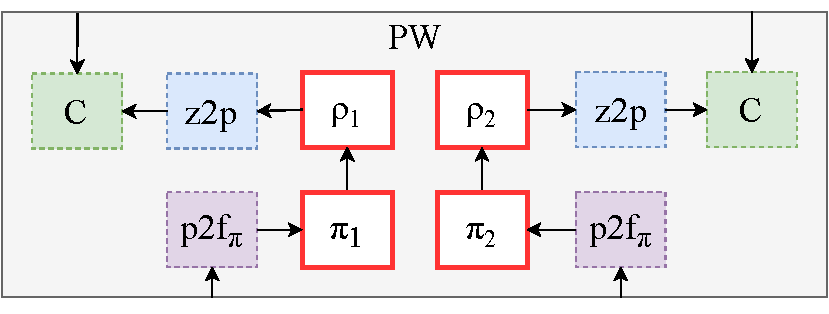
\includegraphics[scale=0.5]{figures/replacement2.pdf}
\caption{When we compose protocols we replace the \emph{p2f} process of $\rho$ with the corresponding instance of $\pi$ and its \emph{p2f} processes. By the emulation theorem, the channel offered by $\rho$ and accepted by $\pi$ have the same type.}
\label{fig:replacement}
\end{figure}

The code for the operator has the same type as any other protocol except, from the description above, it's offered channel is for the type of the functionality $\F_1$ instead of $\F_2$.
We rely on the code generation for to handle spawning instaces of a \inline{p2f} process corresponding to $\pi$ rather than $\rho$.
The operator is given in Figure~\ref{lst:compose}.
\begin{figure}
\begin{lstlisting}[basicstyle=\footnotesize\BeraMonottFamily, frame=single, mathescape]
$\tb{proc}$ compose[K][z,p]:
  (pid: Int), (rng: [Bit]), (sid: session[1]),
  (pid: Int), ($\$$z2p: z) |- ($\$$c: p) =
{
  $\$$ch <- PS.rho <- k rng sid pid $\$$z2p ;
  $\$$c <- Ps.pi <- k rng sid pid $\$$ch 
}
\end{lstlisting}
\caption{The composition operator accepts the same parameters as any other protocol party and offers the channel of type $p2f$ of the realizing protocol $\pi$. We connect $\rho$ to $\pi$ as an environment giving input to $\pi$. We do not need to include any import in our composition operator as the two protocols are guaranteed to be well-matched by the emulation definition. The operator replaces only one party (one \msf{pid}), and the \partywrapper instantiates parties that run the composed protocol.}
\label{lst:compose}
\end{figure}

The resulting composition operator, which composes the two simulators \SIM{\rho} and \SIM{\pi} inside the construction simulator, is best described in text as the resulting code is too verbose to include in the main body of this paper.
You can find the full simulator composition operator in the appendix.
\begin{itemize}
	\item Input from \Z is split between the two simulators
	\begin{itemize} 
		\item \inline{Z2A2P(pid, msg)} intended for parties of $\rho$ are passed to \SIM{\rho}
		\item \inline{Z2A2F(msg)} intended for $\F_1$ is passed to \SIM{\pi}.
	\end{itemize}
	\item Output from \SIM{\pi}: 
	\begin{itemize}
		\item \inline{A2F(msg)} for $\F_2$ and \inline{A2P(pid,msg)} for dummy parties of $\F_2$ are sent to \SIM{\rho} as \inline{Z2A2F(msg)}
		\item \inline{F2A2Z(msg)} is sent to \Z unaltered.
	\end{itemize}
	\item Output from \SIM{\rho}: 
	\begin{itemize}
		\item \inline{A2F(msg)} and \inline{A2P(pid,msg)} for $\F_3$ are sent out unaltered.
		\item \inline{F2A2Z(msg)} messages are sent to \SIM{\pi} as \inline{F2A(msg)} from $\F_2$.
		\item \inline{P2A2Z(pid,msg)} messages are sent to \Z unaltered.
	\end{itemize}
\end{itemize}
The simulator relies on simulators for $\F_1 \xrightarrow{\pi} \F_3$ and $\F_2 \xrightarrow{\rho} \F_3$ to satisfy simulation for Theorem~\ref{thm:singlecomp}.
It is clear that this construction adequately simulates the composed protocol. 
The type in the ideal world gurantees that both the real and ideal world adversaries get at least as much impor as any of the protocol parties. 
This ensures that the composed simulator has enough import to sandbox the two existing simulators and send import out to the ideal world parties and ideal funfctionality.
Therefore it is trivial to see that the composed simulator is well-resource-typed.

Another illustrative description of what composition proposes, logically, is shown by this series of UC executions where the $\equiv$ operator denotes equivalent UC executions that result from moving ITMs in and out of a sandbox, and $\approx$ indicates emulation:
\begin{align}
& \msf{execUC} \: \Z \, (\rho \circ \pi) \, \F_1 \, \DA \\
\equiv \; & \msf{execUC} \: (\Z \circ \rho) \, \pi \, \F_1 \, \DA \\
\approx \; & \msf{execUC} \: (\Z \circ \rho) \, \idealP \, \F_2 \, \SIM{\pi} \\
\equiv \; & \msf{execUC} \: \Z \, \rho \, \F_3 \, (\SIM{\pi} \circ \SIM{\rho})
%\approx \; & \msf{execUC} \: (\Z \circ \Sim{\pi}) \, \idealP \, \F_3 \, \Sim{\rho} \\
%\equiv \; & \msf{execUC} \: \Z \, \idealP \, \F_3 \, (\Sim{\pi} \circ \Sim{\rho}) 
\end{align}

%\item Inputs from \Z of \inline{Z2A2P(msg)} are passed to \SIM{\rho}, and inputs of \inline{Z2A2F(msg)} are passed to \SIM{\pi}.  
%\item \inline{P2A2Z(pid, msg)} outputs from \SIM{\rho} are forwarded to \Z unaltered.
%\item \inline{A2F(msg)} and \inline{A2P(pid, msg)} messages from \SIM{\pi} for $\F_2$ are sent to \SIM{\rho} as \inline{Z2A2F(msg)} and \inline{Z2A2P(pid, msg)}, respectively. 
%\item In the reverse direction, \inline{F2A2Z(msg)} messages from \SIM{\rho} are sent to \SIM{\pi} as \inline{F2A(msg)}, and, finally, \inline{F2A2Z(msg)} output generated by \SIM{\pi} is forwarded to \Z.
%\item \inline{A2P(pid,msg)}, \inline{A2F(msg)} messages from \SIM{\rho}, and \inline{P2A(pid,msg)} and \inline{F2A(msg)} from $\F_3$, are forwarded unaltered. 
%\end{itemize}

%We also provide a composition operator for simulators to construct a simulator for the composed protocol. We connect the simulatorsin the following way
%\begin{figure*}
%\begin{lstlisting}[basicstyle=\small\BeraMonottFamily, frame=single, mathescape]
%$\tb{proc}$ sim_compose[K][a2r,r2a][a2p,p2a][a2f,f2a]:
%  (k: Int), (rnd: [Bit]), (sid: session[1]),
%  (#z_to_a: comm[z2amsg[a2r][a2f]]), (#a_to_z: comm[a2zmsg[r2a,f2a]]),
%  (#a_to_p: comm[a2pmsg[a2r]]), (#p_to_a: comm[p2amsg[r2a]]), (#a_to_f: comm[a2fmsg[a2f]]), (#f_to_a: comm[f2amsg[f2a]])
%    |- ($\$$c: 1) =
%{
%  $\$$ch 
%\end{lstlisting}
%\end{figure*}

%\begin{figure*}
%\begin{lstlisting}[basicstyle=\small\BeraMonottFamily, frame=single,  mathescape]
%$\tb{proc}$ compose[K][z2r][r2z][f2r][r2f][p2f][f2p] : 
%    (pid: Int), ($\$$z_to_p: c[K][z2p]), ($\$$p_to_z: c[K][r2z]), 
%    ($\$$f_to_p: c[K][f2r]), ($\$$p_to_f: c[K][r2f])  |- ($\$$D : 1) =
%{
%	$\$$rho_to_pi <- $\tm{createchan}$[K][p2f];
%	$\$$pi_to_rho <- $\tm{createchan}$[K][f2p];
%
%	 <- pi  <-                 $\$$rho_to_pi $\$$pi_to_rho $\$$p_to_f $\$$f_to_p ;
%	 <- phi <- $\$$z_to_p $\$$p_to_z $\$$rho_to_pi $\$$pi_to_rho ; 
%}
%\end{lstlisting}
%\caption{Composition operator in Nomos that connects a protocol $\rho$ to a protocol $\pi$ that uses some functionality $\F$. The operators creates new channels to connect the realizing $\pi$ and it's hybrid \F. Output from $\rho$ intended for the replace functionality are actually send to parties of $\rho$, and channels outgoing from the parties to the functionality are given to $\pi$.}
%\label{lst:compose} 
%\end{figure*}

%\begin{theorem}[Composition]\label{thm:singlecomp}
%\begin{mathpar}
%\inferrule*[right=single-compose]
%{
%	\F_1 \xrightarrow{\pi} \F_2 \semi \F_2 \xrightarrow{\rho} \F_3 \\
%}
%{
%	\F_1 \xrightarrow{\rho \circ \pi} \F_3
%}
%\end{mathpar}
%
%If \textit{well-typed} $(\pi, \F_1$) realizes $\F_2$ and ($\rho$, $\F_2$) realizes some $\F_3$, then $(\rho \circ \pi, \F_2)$ is \textit{well-typed} and realizes $\F_3$ when $\circ$ is defined as in Figure~\ref{lst:compose}.
%\end{theorem}

%\begin{proof}
%The pre-condition ensures the existence of \textit{well-resource-typed} simulators $\Sim_\rho$ for $\F_2 \xrightarrow{\rho} \F_3$ and $\Sim_\pi$ for $\F_1 \xrightarrow{\pi} \F_2$, and, it is obvious that the composed protocol is also well-resource-typed.
%We construct a simulator \Sim' for the dummy adversary to show
%\[
%	\msf{execUC}\ (\rho \circ \pi)\ \F_1\ \Z\ \A \approx \msf{execUC}\ \idealP\ \F_3\ \Z\ \Sim''
%\]	
%
%The simulator $\Sim'$ relies only simulating \SIM{\pi} and \SIM{\rho}.
%Note that \SIM{\pi} can accept messages for $\pi$ or $\F_1$, simulate them, and generate input for $\F_2$. 
%Similarly, \SIM{\rho} can take inputs for $\rho$ or $\F_2$, simulate them, and generate input for $\F_3$.
%Therefore, we connect the two simulators in the natural way:
%\begin{itemize}
%\item Inputs from \Z of \inline{Z2A2P(msg)} are passed to \SIM{\rho}, and inputs of \inline{Z2A2F(msg)} are passed to \SIM{\pi}.  
%\item \inline{P2A2Z(pid, msg)} outputs from \SIM{\rho} are forwarded to \Z unaltered.
%\item \inline{A2F(msg)} and \inline{A2P(pid, msg)} messages from \SIM{\pi} for $\F_2$ are sent to \SIM{\rho} as \inline{Z2A2F(msg)} and \inline{Z2A2P(pid, msg)}, respectively. 
%\item In the reverse direction, \inline{F2A2Z(msg)} messages from \SIM{\rho} are sent to \SIM{\pi} as \inline{F2A(msg)}, and, finally, \inline{F2A2Z(msg)} output generated by \SIM{\pi} is forwarded to \Z.
%\item \inline{A2P(pid,msg)}, \inline{A2F(msg)} messages from \SIM{\rho}, and \inline{P2A(pid,msg)} and \inline{F2A(msg)} from $\F_3$, are forwarded unaltered. 
%\end{itemize}
%It is clear that \Sim' is able to emulate inputs from \Z to both parties of $\rho$ and the ideal functionalty $\F_1$.
%\Sim' performs constant over head in simulating two \emph{well-resource-typed}, and therefore it is clear that \Sim' is \emph{well-resource-typed}.
%When combined with the \emph{dummy lemma}, a well-resource-typed simulator exists for composition for any adverasry \A. 
%The dummy lemma presented above ensures that a simulator for any \A can be constructed that is well-resource-typed for all wel-resource-typed \A.
%\end{proof}
%
%We give a simpler, high-level idea of the forst step of the proof proof here which can be understood visually:
%The $\equiv$ operator is a result of moving around ITMs (some from within other ITMs into the main UC execution) and $\sim$ refers to indistinguishability.
%In line (13) above, $\rho$ is moved into the execution environment with an unchanged simulator as no additional simulation is required: the simulator allows unfettered communication between parties of $\rho$ and \Z.

\subsection{Multisession}

\begin{theorem}[Composition]\label{thm:composition}
\begin{mathpar}
\inferrule*[right=compose]
{
	%(\pi, !\F_1) \sim (\idealP, F_2) \semi (\rho, !\F_2) \sim (\idealP, \F_3) \\ 
	!\F_1 \xrightarrow{\pi} \F_2 \semi !\F_2 \xrightarrow{\rho} \F_3 \\
	%\Rightarrow \exists \Sim(\A) \vdash (\rho^{!\F_2 \rightarrow (!\pi \, \circ \, \msf{squash})}, !\F_1) \sim (\idealP, \F_3)
}
{
	!\F_1 \xrightarrow{\rho \, \circ !\pi \circ \, \msf{squash}} \F_3
	%(\rho \, \circ \, !\pi \circ \msf{squash}, !\F_1) \sim (\idealP, \F_3)
}
\end{mathpar}
\end{theorem}
Full composition in the UC framework extends beyond the simpler composition in Theorem~\ref{thm:singlecomp} which only defines replacement of one functionality with a protocol that realizes it.
Instead, UC composition allows for replacement of any number of instances of a functionality with instancesof the realizing protocol.
Theorem~\ref{thm:composition} illustrates the full composition theorem using our arrow notation, and highlights a theorem that we must prove before we can achieve full composition.
It relies on Theorem~\ref{thm:squash} that introduces the \msf{squash} protocol and the $!$ operator.
Notice that Theorem~\ref{thm:compose} follows directly from Theorem~\ref{thm:singlecomp} and Theorem~\ref{thm:squash}.

The multi-session extension of a protocol or functionality, specified by the $!$ operator (such as $!\rho$ or $!\F$), allows multiple instances of the protocol/functionality to be run within a sinlge ITM.
An ITM simulates the instances and multiplexes input/output to/from them much like the \partywrapper.

\begin{theorem}[Squash Theorem]\label{thm:squash}
%If a functionality \F is well-resource-typed, then $!\F$ and $!!\F$ are well-resource-typed (by Theorem~\ref{thm:bangppt}) and $(\idealP, !!\F) \sim (\msf{squash}, !\F)$.
%\textit{Well-resource-typed} \F $\Rightarrow$ $!\F \xrightarrow{\msf{squash}} !!\F$%  $(\idealP, !!\F) \sim (\msf{squash}, !\F)$
\begin{mathpar}
\inferrule*[right=squash]
{
\textit{well-resource-typed} \; \F
}
{
!\F \xrightarrow{\msf{squash}} !!\F
}
\end{mathpar}
\end{theorem}

For the multisession extension of a fuctionality, the type is straightforward and ony acts to multiplex input/outpt based on the intended target \inline{ssid}.
\begin{center}
\parbox{0cm}{
\begin{tabbing}
$\m{{P2MS}[a,b]\{n,m\}} = \textcolor{red}{\getpot^n} \ichoice{\mb{Inp}: ssid \arrow a \tensor \echoice{$\=$\mb{Ok}: \textcolor{red}{\paypot^0} \; \m{P2MS[a,b]\{n,m\}},$ \\
\>$\mb{Out}: ssid \arrow b \tensor \textcolor{red}{\paypot^m} \; \m{P2MS[a,b]\{m,n\}}}}$
%\m{MS2P[a][b]\{n,m\}}}$ \\
%\mi{stype} \; \m{{MS2P}[a][b]\{n,m\}} = \echoice{\mb{Ok}: \textcolor{red}{\paypot^0} \; \m{P2MS[a][b]\{n,m\}}, \mb{Out}: ssid \product b \arrow \textcolor{red}{\paypot^m} \; \m{P2MS[a][b]\{n,m\}}}  
\end{tabbing}}
\end{center}
The multisession extension is mentioned in greater detail in the appendix.
%and the functional types that are sent to the wrapper surrounding it are given by
%\begin{lstlisting}[basicstyle=\small\BeraMonottFamily, mathescape]
%$\yo{type}$ p2ms[a] = P2MS of ssid ^ a ;
%$\yo{type}$ ms2p[b] = MS2P of ssid ^ b ;
%\end{lstlisting}
%It is important to note that we require a session type here instead of allowing !\F act as the functionality wrapper because, when composed it must communicate directly communicate, over a session-typed channel, to another protocol.
%Furthermore, the construction of !\F is the same as in the \Fro example: one session typed channel for all parties.
%In Figure~\ref{fig:multisession} illustrated the functionality wrapper (right) and the multisession extension (left) for \Fcom. 
%\begin{figure}
%\centering
%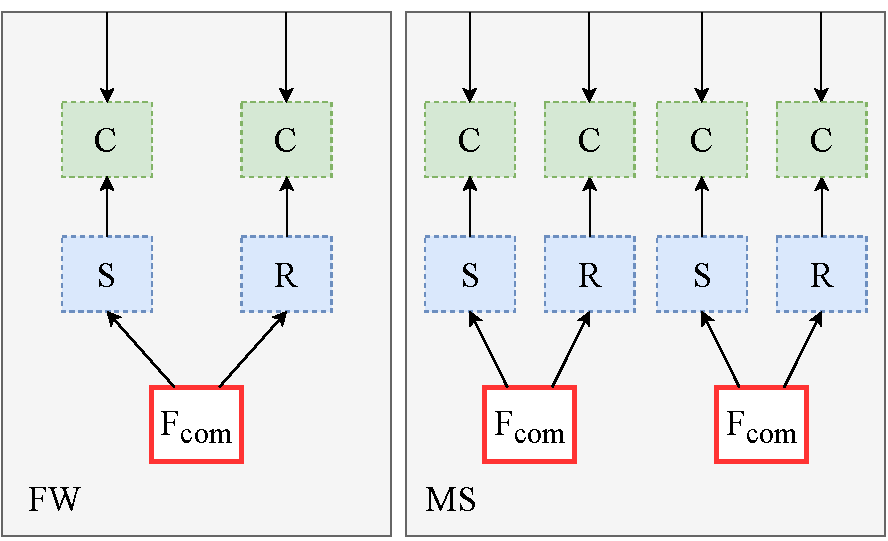
\includegraphics[scale=0.5]{figures/multisession.pdf}
%\caption{The multisession extension of \Fcom (right) with only two instances, creates the same processes $S$ and $R$ (offering the session typed channel to \Fcom) for every created instance. A communicator per session buffers messages for the $S$ and $R$ processes to consume and forward along their session-typed channel to \Fcom.}
%\label{fig:multisession}
%\end{figure}

%As a generic construction provided by NomosUC, the multisession operator requires some code generation but only to accept an arbitrary number of virtual token types if the underlying \F simulators other processes. 
%Furthermore, similar to the functionality wrapper, the multisession operator constructs the processes around \F in the same way and spawns them on-demand.
%The process definition for $!\F_\msf{com}$ is shown in Figure \ref{lst:bangf} accepting two token types: the real token type $K$ and the virtual token type $K_1$ for instances of $\F_\msf{com}$.
%
%\begin{figure}
%\begin{lstlisting}[basicstyle=\footnotesize\BeraMonottFamily, frame=single, mathescape]
%$\tb{proc}$ bangF[K,K1][p2f,...] :
%  (k: $\tgr{Int}$), (rng: [Bit]), (sid: session[a]), 
%  ($\$$p: P2MS[p2f][f2p]) |- ($\$$ch: 1) =
%\end{lstlisting}
%\caption{The type definition for the multisession operator for functionalities and the correspond message type and import parameters. The operator for protocol parties is identical in code but differens in that the parameters to the \texttt{P2MS} type are for \texttt{Z2P} interaction.}
%\label{lst:bangf}
%\end{figure}

\begin{theorem}[PPT !]\label{thm:bangppt}
If a functionality $\F$ is well-resource-typed, then it's multisession extension $!\F$ is well-resource-typed.
\end{theorem}

We examine this theorem in greater detail in the appendix. 
At a high-level it is obvious that such a construction, activated polynomially many times, is well-resource-typed as long as the underlying functionality/protocol is well-resource-typed.
%\begin{proof}
%A \textit{well-resource-typed} \F guarantees a polynomial $T_{\F}$ bounding its execution.
%In the worse-case, the multisession operator must spawn a new instance of $\F$ an every activation. 
%Let $N_{\F}$ denote the total number of instances (and, hence, number of activations) of $\F$ created by the operator.
%Note that $N_{\F}$ is polynomial in the security parameter $k$ for all well-typed environments, protocols, and adversary.
%Therefore, there always exists a bounding polynomial to bound a polynomial number of simulated instances of \F.
%The polynomial can be given as:
%$$ P_{!\F}(n) = N_{\F} P_{\F}(n) + \mathcal{O}(N_{\F}) $$
%where the $\mathcal{O}(N_{\F})$ is due to the overhead of maintaining and accessing the set of all instances.
%
%Similarly, \F being \textit{well-resource-typed} ensures a valid token context for all processes it may simulate. 
%Therefore, it is clear that there exists a global connecting poltnomial $f$ that ensures a valid token context for $!\F$.
%\end{proof}


%\begin{figure}
%\begin{lstlisting}[basicstyle=\small\BeraMonottFamily, mathescape, frame=single]
%$\yo{type}$ p2bFmsg[a] = P2bF of ssid ^ a ;
%$\yo{type}$ p2bbFmsg[a] = P2bbF of ssid ^ ssid ^ a ;
%$\tg{(* z2p : comm[z2pmsg[p2bbf[a]]] *)}$
%$\tg{(* p2f : comm[p2fmsg[P2bf[a]]] *)}$
%pid = recv $\$$z2p ;
%m = recv $\$$z2p ;
%case m (
%  P2bbF(ssid1, ssid2, m) =>
%    send $\$$p2f P2bF(ssid1 + ssid2, m) ;
%)
%\end{lstlisting}
%\caption{The \textit{squash protocol} accepts a message intended intended for $!!\F$ of type \inline{P2MS[p2ms[a]][ms2p[b]]}, i.e. of the form $(\msf{ssid}_1, (\msf{ssid}_1, msg))$.
%It ``flattens'' it into a single $\msf{ssid}_3 = \msf{ssid}_1 + \msf{ssid}_2$ that can be passed to $!\F$. The result is the same number of instances of \F but behind only a single $!$ operator.}
%\label{fig:squash}
%\end{figure}

\begin{proof} (Theorem~\ref{thm:squash})
On examination the \msf{squash} theorem does constant work per activation and concantenates two \inline{ssid}s into one for messages going to the functionality and does the inverse for messages incoming from the functionality.
We provide more detail for a proof of Theorem~\ref{thm:squash} in the Appendix, however, it is clear to see that the this theorem holds with a trivial simulator.
%First we describe the \msf{squash} protocol where $!!\F$ are nested $!$ operators.
%The protocol accepts messages intended for $!!\F$ of type \inline{P2MS[p2ms[a]][ms2p[b]]}, i.e. of the form $(\msf{ssid}_1, (\msf{ssid}_2, msg))$, and ``flattens'' them into a single message of type $\inline{P2MS[a][b]}$, i.e. of the form $(\msf{ssid}_3, msg)$.
%
%In $(\idealP, !!\F)$, \idealP~expects to receive messages of the form $(\msf{ssid}_1, (\msf{ssid}_2, m))$ where $\msf{ssid_2}$ is a sub-session of $\F$ (i.e. instance) inside some $!\F$ with sub-session id $\msf{ssid}_1$ inside of $!!\F$ (the message accesses functionality $\F[\msf{ssid}_1][\msf{ssid}_2]$).
%The \msf{squash} protocol flattens the indexing of instances of \F and combines session ids $\msf{ssid}_1$ and $\msf{ssid}_2$ into a single \msf{ssid}: $\msf{ssid}_3 := \msf{ssid}_1 \cdot \msf{ssid}_2$.
%If follows intuitively that the view for the environment remains the same. 
%
%We construct a simulator such that:
%\[
%\msf{execUC} \, \Z \, \idealP \, !!\F \, \SIM{\msf{squash}} \approx \msf{execUC} \, \Z \, \msf{squash} \, !\F \DA 
%\]
%The simulator is very simple. 
%Inputs to/from parties/\Z for a corrupt party is forwarded unmodified.
%Input intended for $!\F$ of the form $(\msf{ssid}_1 \cdot \msf{ssid}_2, msg)$ is sent as $(\msf{ssid}_1, (\msf{ssid}_2, msg))$ to $!!\F$. 
%Output from $!!\F$ is modified inversely and sent to \Z.
%
%The proposed simulator is trivially analyzed to be \textit{well-resource-typed}.
%It performs constant work per activation and does ``real'' simulation other than message modification to/from $!!\F$.
\end{proof}

\subsection{UC Composition}
Finally, we can conlude with full composition in Theorem~\ref{thm:compose}.
The proof follows directly from Theorems~\ref{thm:singlecomp} and \ref{thm:squash}.

\begin{proof}
By Theorem~\ref{thm:singlecomp} we can construct a simulator \SIM{1} for $!!\F_1 \xrightarrow{\rho \, \circ \, !\pi} \F_3$.
Theorem~\ref{thm:squash} then allows us to ``squash'' $!!\F_1$ and construct a simulator using \SIM{1} for $!\F_1 \xrightarrow{\rho \, \circ \, !\pi \, \circ \, \msf{squash}} \F_3$
\end{proof}

\subsection{Design Discussion}
One of the core research questions that this work aims to study session types applied to the UC framework. 
In this section, we discuss how resource-aware session types impact the design of functionalities in NomosUC as well as which are implementable.
We use the two-way authenticated channel functionality \Fauth to througout this discussion.

In plain session types, communication between two parties $P_s$ and $P_r$ occurs over a single duplex channel.
In UC the role of the adversary as a message scheduler in \Fauth, the most common network channel model, means a more complicated functionaty involving $P_s$, $P_r$, \F, and \A. 
The simplest, and most common approach, to \Fauth is the following communication pattern: a party $P_s$ sends a message to \Fauth, \Fauth sends the message to \A and waits for \A to say \inline{OK} before delivering the message to $P_r$.
Since both parties can send a message and receive a message, it is unclear which process, \Fauth or $P$, will be active along that channel at any given time.
Session types require this information to be statically known when two processes are communicating over a single channel--making this communication pattern unexpressable over a single channel.

There a few ways to overcome this constraint. 
In general, even though the UC framework places few restructions of communication patterns, most functionalities stick to a few.
\Fauth, for example, can take a few forms:
\begin{enumerate}
\item (presented above) Receiver and adverasry are activated directly: \Fauth waits for \A to tell it to deliver the message.
\item \Fauth ``polling'' approach: messages from $P_s$ are buffered for both \A and $P_r$. \A and $P_r$ must ask \Fauth for new messages. This is a more invonconvenient method, but can be useful for novel functionality designs that need a channel.
\item ``polling'' but receiver is activated: the message is stored in a buffer for \A, and \A's deliver message directly sends it to $P_r$.
\end{enumerate}
The simplest way to implement \Fauth in NomosUC is ``polling'' approach. As far as we know, we can systematically tranform any UC functionality into one that uses ``polling''. 
The consequences are that polling is inconvenient from a programming point of view because \Z needs to continuously activate parties to ask for new messages.
Hope is not lost though, because it turns out our type system can express functionalities in all three of the ways listed above. 
The first, and most natural, approach only requires splitting communicating between $P$ and \Fauth into two unidirectional channels
Such an extension to NomosUC trivially modifies the \partywrapper to handle two channels instead of one, and the types of the channels can be succintly expressed as: 
\begin{center}
\parbox{0cm}{
\begin{tabbing}
$\m{sending}[a] = \textcolor{red}{\getpot^n} \ichoice{\mb{sendmsg}: \m{a} \tensor \m{sendmsg}}$ \\
$\m{receive}[a] = \textcolor{red}{\getpot^m} \echoice{\mb{recv}: \m{a} \tensor \m{receive}}$ \\
$\m{adv}[a] = \echoice{\mb{leakmsg}: a \tensor \ichoice{ \mb{ok}: \m{leakmsg}}}$
\end{tabbing}}
\end{center}
The first to correspond to the channels for sending from $P$ to \Fauth and the second in the opposite direction. The third is the adversary's channel at \Fauth.

A notable part of our contruction is the machinery created around the protocol parties and functionality that intemediate their communication with communicators and functionally-typed messages.
Recall that such compromises are required in order to allow a \emph{dynamic} number of parties in UC.
The session type of the shared channel of a communicator only allows for a fixed amount of import to be sent over it with every messages. 
Protocols and functionalities that send different amounts of import depending on the message, say $i_1,...,i_n$, must now send $\m{max}(\{i_j\})$ import with every messages.
For existing UC definitions this appears to be an issue of ensuring a machine has \emph{enough} import, however, we can systematically map any UC import definition to one that works in NomosUC~\footnote{The problem can be reduced to ensuring enough ``latent'' import needed to compute, and, because we aren't concerned here with \emph{tight} computational bounds the problem is quite easy to solve. We discuss in greater detail in the appendix.}.



%\caption{The \msf{execUC} function used for the two-party commitment example used througout this paper. Recall, the \msf{execUC} is customized insofar as it takes in some number of virtual token types (here, $K_1$) to enable machines that simulate other machines. In the commitment example, there is no such simulation happening at the protocol or functionality level, therefore only the real token type $K_1$ is used here. The funtion spawns all the necessary ITMs in the UC execution: the environment, the protocol wrapper, the functionalty (wrapped), and the adversary. Each is parameterized with the security parameter $k$ and a random bit sequence $\msf{rng} \in \{0,1\}^{poly(k)}$.
%At the end, the environment is started and it returns a bit $b$ which is its guess for which world it is in. The full code can be found in the Appendix.}
%\label{lst:execuc}
%\end{figure*}

%We separate NomosUC into two modules: generic code and protocol-specific code. 
%Therefore, the \inline{execUC} refers to user specified code through the \inline{PS} module which defines \inline{PS.env} for \Z, \inline{PS.func} for the functionality, \inline{PS.prot} for the protocol, and \inline{PS.adv} for the adversary.
Communication between all of the major processes in the UC execution (\Z, \A, \partywrapper, and \fwrapper) is done through communicators introduced in Section~\ref{sec:nomosuc}.
Communicators are restricted to only sending functionally types messages in NomosUC, and we give generic types, below, to all such messages.
\todo{Is this important to even have here? seems a useless implementation detail.}
\begin{lstlisting}[basicstyle=\footnotesize\BeraMonottFamily, frame=single, mathescape]
$\Type$ p2zmsg[a] = P2Z of pid ^ a ;
$\Type$ p2fmsg[a] = P2F of pid ^ a ;
$\Type$ f2pmsg[a] = F2P of pid ^ a ;
\end{lstlisting}

\paragraph{The Environment}
The environment is the first machine that \inline{execUC} spawns and receives from it the session id and list of corrupted parties for this execution.
Its offered channel type \inline{EtoZ} specifies the interaction between \inline{execUC} and \Z:
\begin{lstlisting}[basicstyle=\footnotesize\BeraMonottFamily, mathescape, frame=single]
$\Type$ EtoZ[a] = +{init: a ^ list[pid] -> exec} 
$\Type$ exec = &{start : output_bit} ;
$\Type$ output_bit = +{bit: Bit -> 1} ;

$\tb{proc}$ PS.env[K][z2p,...]{p2zn,...} : 
  (k: $\tgr{int}$), (r: [Bit]), (#ztop: comm[z2pmsg[z2p]]{z2pn}), 
  (#ptoz: comm[p2zmsg[p2z]]{p2zn})...  |- ($\$$z : EtoZ) $\tg{(* <- offered channel *)}$
\end{lstlisting}
The environment also accepts communicators, as parameters, for communication with the protocol parties and the adversaries (in both directions), and offer a channel \inline{$\$$z} of type \inline{EtoZ}.
The type (above) states \Z provides an \emph{sid} of some user-defined type \inline{a} and a list of the \emph{pid}s of corrupted parties. 
Finally, \inline{execUC} instructs it to \inline{start} (\emph{external choice}) and return a bit $b$ as its guess for which world it is in.

%The \inline{\{z2pn\}}, for example, specifies the amount of import that must be sent by \Z with every message to a protocol party.
%The rest of the processes---the adversary, protocol wrapper, and functionality--are declared in the same way except the type parameters they expect are different: the protocol wrapper would of course accept type parameters for communication between it and \F, \A, and \Z.
%Finally the type of the offered channel \inline{$\$$z} is the same for all environments and communicates the \inline{sid} and set of corrupt parties chosen by \Z to \inline{execUC}.
%The \inline{sid} and corrupt list are parameters to the rest of the processes that \inline{execUC} spawns. 

%The communicators created by \inline{execUC} always use the same parametric types. 
%For example, for communication with the protocol, the types look like:
%\begin{lstlisting}[basicstyle=\small\BeraMonottFamily, frame=single, mathescape]
%$\Type$ p2zmsg[a] = P2Z of pid ^ a ;
%$\Type$ p2fmsg[a] = P2F of pid ^ a ;
%$\Type$ f2pmsg[a] = F2P of pid ^ a ;
%\end{lstlisting}
%Subsequently, the channel from \Z to the protocol wrapper will be typed as: \inline{comm[z2pmsg[z2p]]\{z2pn\}} where \inline{z2p} is a protocol-specific message type.
%The protocol \inline{PS.prot} is not spawned by \inline{execUC}. Instead the process spawns the protocol wrapper (described below) which spawns parties with that run the code \inline{PS.prot}.
%When in the ideal world, the protocol is given as the ideal protocol: one where the protocol wrapper converts the message from type \inline{z2pmsg[a]} to type \inline{p2fmsg[a]} but forwards the contents unaltered.
%The protocol wrapper and functionality wrapper manage spawning the instance(s) of the functionality and protocol parties.
%Similarly, an environment \msf{PS.env} and adversary \msf{PS.adv} must be defined as well.
%The message types exchanged between the processes are provided directly to \msf{execUC} as type parameters of the form \msf{p2f}, \msf{f2p}, and so on. 
%The first thing \inline{execUC} does is create the communicators and the corresponding channels for the main processes of the execution. 

%A consequence of using communicators is that in the UC setting they require at least 1 unit of import, beacuse they are activated a potentially polynomial number of times. 
%Therefore, all communicators in NomosUC receive some amount of import $n$ and send out only $n-1$. 
%The user-specified protocol, environment, functionality, and adverasary must account for this to ensure suffiient import is given to them.
%\begin{lstlisting}[basicstyle=\small\BeraMonottFamily, frame=single, mathescape]
%#ptoz <- communicator_init[K][p2zmsg[p2z]]
%           {p2zn+1} ;
%#ztop <- communicator_init[K][z2pmsg[z2p]]
%           {z2pn+1} ;
%...
%\end{lstlisting}
%This is strictly a design decision where user-defined protocols only specify import token requirements for the protocol not taking communicators into account. 
%The processes that they write, though, must conform to this standard and send an import token in addition to the amount they need.
%An alternate design would be that all import type parameters take the additional import token into account and communicators send one less than they receive.
%The drawback of the latter approach is that that when communicating with a process directly rather than through communicators (say, when simulating), you're sending one extra token for no reason.

%Next, the environment \msf{PS.env} is spawned, \inline{execUC} receives the \inline{sid} and corrupt list from \Z, and, finally, the remainder of the processes are spawned with these inputs. 
%Finally, the environment executes its own code when activated by \msf{\$z.start}, given the initial amoutn of import \inline{n}, and returns a bit through \inline{$\$$z.output_bit} which is its guess whether it's in the real or ideal world:
%\begin{lstlisting}[basicstyle=\small\BeraMonottFamily, frame=single, mathescape]
%$\$$z.start
%$\tb{pay}$ $\$$z {n}
%$\$$d <- $\$$z
%\end{lstlisting}

\subsection{The \partywrapper}
NomosUC departs slightly from the standard UC framework by using a \partywrapper to encapsulate all protocol parties and run them internally.
Rather than passing protocol party channels as parameters to \Z or \A (supporting a static set of parties), the \partywrapper provides a single endpoint for all messages to parties.
Similarly we adapt a \fwrapper to function like the \partywrapper but on functionalities. The main pupose of this wrapper and the \partywrapper is to intermediate communication between the session types the functionality uses and the functionally typed messages exchanges through communicators.

Like \iexecuc, we genrate the \partywrapper based on the protocol or functionality being executed. 
Converting between functional and session-typed messages is an easy task to automate and we push that onto code generation rather than requiring a user to produce it.
The extra processes generated within the \partywrapper are shown in Fiure~\ref{fig:blankpartywrapper}.
%In a nutshell, the wrapper accepts messages from a communicator, say from \Z, demultiplexes it, converts its type to one over a session-typed channel and conveys it to the necessary protocol party.

Following along with Figure~\ref{fig:blankpartywrapper}, the generated processes \inline{C} are use to de-multiplex messages based on the \inline{pid} of the receipient, and the \inline{z2p} and \inline{p2f} processes convert messages between the session typed channels and the functional messages that are received.
The arrow notation in Figure~\ref{fig:blankpartywrapper} indicates the $\m{prodiver} \leftarrow \m{client}$ relationship for each channel and provides their types.

We elaborate on the processes \inline{z2p}. For the commitment protocol the messages received by the \partywrapper are type as 
\begin{lstlisting}[basicstyle=\footnotesize\BeraMonottFamily, mathescape]
$\yo{type}$ comp2f = Commit of Bit | Open ;
$\yo{type}$ comf2p = Committed | Open of Bit ;
\end{lstlisting}
and the \inline{z2p} process intercepts them and communicates to the party over a channel typed with the \Fcom session types in Section~\ref{sec:nomosuc}.
For example when \Z gives the command to commit to a bit, \inline{z2p} does the following:
\begin{lstlisting}[basicstyle=\footnotesize\BeraMonottFamily, frame=single, mathescape]
case msg (
  Commit(b) =>
    $\$$z2p.commit ;
    $\tb{send}$ $\$$z2p b ;
    $\tb{pay}$ {z2pn} $\$$z2p ;
\end{lstlisting}
where \inline{$\$$z2p} is the session-typed channel to the committer.
The \inline{f2p} processes does the same for communication between the parties and the functionality.

Virtualizing the protoocl parties means that the wrapper and the parties it runs are, effectively, using the same import and potential.
We reason that the \partywrapper and protocol parties it runs will always have enough import by noticing that the \partywrapper does constant work on each activation.
Therefore, if protocol parties intend to hold on to import, there is always a suficient polynomial to allow both the wrapper and the party to perform potentially polynomial computation.
\todo{Reword this to make it crisper}.

%Folling along with Figure~\ref{fig:blankpartywrapper}, the generatd processes \inline{z2p} and \inline{f2p} communicate with the party over a session-typed channel and perform the message type conversion mentioned above based on a simple message type mapping provided by the user.
%The \inline{z2p} process offers a linear channel to the party with the correct session type with \Z. 
%The wrapper reads messages from \Z, demultiplexes them based on \inline{pid} and puts them in the appropriate virtual communcator (the green box labeled \inline{C}) for the \inline{z2p} processes to read from, convert, and send to the party.
%The protocol party offers a linear channel of its type with \F, and \inline{p2f} converts this to a functional type. \inline{p2f} offers the same type as a communciator to the wrapper which reads the message and sends it to \F. 
%Figure~\ref{fig:blankpartywrapper} indicates the type of the offered channel for all the relevant processes within the wrapper. 

%In order to use session types, the each protocol party is internally connected to two processes \inline{z2p} and \inline{f2p} over with session-typed channels for their communication with \Z and \F, respectively.
%\inline{z2p} is connected to party-specific virtual communicators so that \inline{z2p} and \inline{f2p} can read/send messages from. It can not read/write directly to/from the actual communicators connecting the protocol wrapper because, being simulations inside the protocol wrapper, they do not use the same token type.
%In the case of the ideal world with \Fcom, the both of the sender's ($\pi_1$) channel with \inline{z2p} channels with \inline{z2p} and \inline{f2p} are typed as \inline{sender}, and the protocol party itself ($\pi_1$) just fowards messages from one channel to the other.

%The processes \inline{Z2p} and \inline{f2p} are generated for each party based on their session-type, and they convert between them and functional messages for incoming/outgoing communcation with \Z, \F, or \A. 
%For example in the commitment example, where the functional message type is given by: 
%\begin{lstlisting}[basicstyle=\footnotesize\BeraMonottFamily, mathescape]
%$\yo{type}$ comp2f = Commit of Bit | Open ;
%$\yo{type}$ comf2p = Committed | Open of Bit ;
%\end{lstlisting}
%the \inline{z2p} process does something like this for the sender (where \inline{msg} is received from its virtual communicator):
%\begin{lstlisting}[basicstyle=\footnotesize\BeraMonottFamily, frame=single, mathescape]
%case msg (
%  Commit(b) =>
%    $\$$z2p.commit ;
%    $\tb{send}$ $\$$z2p b ;
%    $\tb{pay}$ {z2pn} $\$$z2p ;
%\end{lstlisting}
%It sends a commit message over the linear channel with the sender, and pays the necessary amount of (virtual) import tokens with the message.
%When \Z, \A, or \F send a message to a party that doesn't exist, the \partywrapper creates the new party's \inline{z2p}/\inline{f2p} processes and an instance of the party itself, and it connects them together in the same way shown. 
%We do something similar for functionalities, in Appefix~\ref{app:fwrapper}

\begin{figure}
\centering
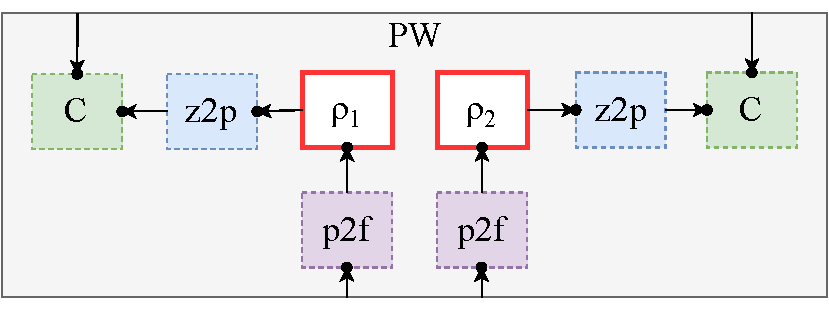
\includegraphics[scale=0.5]{figures/blankpartywrapper2.pdf}
\caption{The internals of the protocol wrapper with two parties. The arrows indicates the client/provider relationship between each pair: provider $\rightarrow$ client. The wrapper creates \texttt{z2p} to offer a channel and convert from gunctional to message type---the \texttt{p2f} do the same. A communicator is used because \texttt{z2p} cannot send message to real one with differing token type. The types of the processes offered are (color): \tgr{comm[z2pmsg[comp2f]]}, \tb{sender}, \tr{party[Int]}, \tp{comm[p2fmsg[rop2f]]}. }
%The processes \texttt{z2p} offer linear channels to their respective protocol parties that are typed according to that party's protocol, and they receive messages from virtual communicators that hold messages specific to one \texttt{pid}. The protocol code for $\pi_1$ and $\pi_2$ are user-specified and offer a channel to the \texttt{p2f} process according to their protocol with the functionality. The \texttt{p2f}s convert outgoing messages to, and incoming messages from, functional message types to be sent to/from the functionality. The protocol wrapper gives messages to the virtual communicators and receives messages from \texttt{p2f}s.}
\label{fig:blankpartywrapper}
\vspace{-1.5em}
\end{figure}

%For the commitment example, if $\pi_1$ and $\pi_2$ ran the commitment protocol, \inline{z2p} would offer a channel of type \inline{sender} and \inline{receiver} to $\pi_1$ and $\pi_2$, respectively, and it converts between the functional messages for the commitment protocol and the session typed ones. 
%In the ideal world, the $\pi_1$ and $\pi_2$ run a dummy protocol where their offered channels are simply forwarded to their \inline{z2p} channels, i.e. the \inline{z2p} and \inline{f2p} channels have the same type: \inline{sender} and \inline{receiver}, respectively.
%In the style of Nomos, the protocol wrapper:
%\begin{itemize}
%	\item Attempts to read messages incoming from \Z, \A, or \F and forward them to the appropriate process depending on \inline{pid}.
%	\item Read from the internal communicators or the \inline{p2f} processes for outcoing messages.
%\end{itemize}
%For reference the functional messages typed for the commitment protocol are:

%Recall the session types for the sender and receiver, with \Fcom, introduced in Section \ref{subsec:idealcommitment}.
%%\begin{gather}
%%	\mi{stype} \; \m{sender} = \ichoice{\mb{commit} : \m{bit} \product \m{scommitted}} \\
%%	\mi{stype} \; \m{scommitted} = \ichoice{\mb{open} : 1} \\
%%	\mi{stype} \; \m{receiver} = \echoice{\mb{commit} : \m{rcommitted}} \\
%%	\mi{stype} \; \m{rcommitted} = \echoice{\mb{open} : \m{bit} \arrow \one}
%%\end{gather}
%At the beginning there are no parties. When the \A or \Z write to a party with some pid $p$ the protocol wrapper creates $p$ if it does not exist.
%It creates and stores the session-typed channels or all of the parties in channels corresponding to their type and moves channels between them as the type evolves.
%For example for parties' channel with \Z the protocol wrapper generates the following lists:
%\begin{gather}
%	\m{R1L1}[\m{sender}] \\
%	\m{R1L2}[\m{scommitted}] \\
%	\m{R2L1}[\m{receiver}] \\
%	\m{R2L2}[\m{rcommitted}] 
%\end{gather}
%At the beginning of the protocol, the committer's \msf{z2p} channel would be in \inline{R1L1} and the receiver's is in \inline{R2L1}.
%The channel's connection the protocol wrapper to the rest are still functionally typed. It's channel \inline{p2f} will still be typed \inline{#ptof: comm[p2fmsg[comp2f]]} where \inline{comp2f} is:
%Succinctly, the protocol wrapper functions as follows:
%\begin{itemize}
%\item When the protocol wrapper receives a message for some \msf{pid}, if the party doesn't exist the protocol wrapper creates all the party's channel parameterized by the correct session types (the role of the party is determined by the incoming message). The channels are stored and outgoing channels are waiting to be read from.
%\item The message sent to the party with the session type is determined by the functional type. The wrapper creates a session-typed message and forwards the contents of the message to the party.
%Despite accepting functionally typed messages, the protocol wrapper uses session types in this way to allow the type checker to catch invalid and out of order environments, adversaries and functionalities. 
%For example, in the commitment protocol when the committer tries to commit a bit in \Fcom like this:
%\begin{lstlisting}[basicstyle=\small\BeraMonottFamily, frame=single, mathescape]
%$\$$p2f.commit 
%$\tb{send}$ $\$$p2f b
%$\tb{pay}$ {p2fn} $\$$p2f
%\end{lstlisting}
%\begin{lstlisting}[basicstyle=\small\BeraMonottFamily, frame=single, mathescape]
%$\$$p2f.SEND 
%$\tb{send}$ $\$$p2f pid 
%$\tb{send}$ $\$$p2f Commit(b)
%$\tb{pay}$ {p2fn} $\$$p2f
%\end{lstlisting}
%The party wrapper intercepts and converts it to a functionally typed message:
%\item For outgoing messages, the protocol wrapper does a similar conversion where it reads the sesion typed channel output by the party and converts its message to the appropriate functional message type.
%\end{itemize}

%\paragraph{Functionality Wrapper}
%The \fwrapper adopts a similar approach to the \partywrapper, except it only creates one instance of the underlying functionality.
%For the same reason as the \partywrapper, we use an \fwrapper to enable a dynamic set of parties.
%One caveat in supporting such functionalities, is that, so far, only functionalities whose type follows a specific form are allowed.
%In the random oracle type given below, notice that the type before and after a party interacts with it is the same: type $\m{party}[a]$.
%\begin{mathpar}
%\m{party}[a] = \textcolor{red}{\getpot^1} \ichoice{\mb{hash} : \m{pid} \arrow \m{int} \product \m{hashing}[a]} \\
%\m{hashing}[a] = \echoice{\mb{shash} : \m{pid} \arrow \m{int} \product \textcolor{red}{\paypot^0} \m{party}[a]} 
%\end{mathpar}
%A party queries a $\mb{hash}$ of an integer from \Fro and receives an integer as a response. The session type includes the \inline{pid}, which enables it to handle all parties over the same channel.
%
%An example of the internals of the \fwrapper are showing on the left-hand-side of Figure~\ref{fig:multisession}.
%Like the \inline{z2p} processes in the \partywrapper, \inline{S} and \inline{R} represent the sender and receiver in the commitment protocol, and they read from their virtual communicators and communicate with \Fcom over a session-typed channel.

%When a party invokes \Fro, the type it expects is \inline{party[a]}, and when it has received its hash the type is again back at \inline{party[a]}. 
%The wrapper handles such dynamic functionalities by channeling all party communication through one linear channel in the wrapper. 
%Therefore, \Fro reads on one channel and responds to the specific party with some \inline{pid}, and the protocol wrapper remains unchanged. 
%
%The constructions of the protocol wrapper and functionality wrapper enable users to write very simple ideal functionality and protocol code, as we will discuss in the next Section and in the Appedix.

%In the commitment example, \Fcom accepts two channels, one from each party, and two processes are created (call then \inline{p2f} for now) which offer channels of type \inline{sender} and \inline{receiver}, respectively. 
%The wrapper differs from the protocol wrapper for certain functionalities that accept a dynamic number of parties. 
%Continuing with our commitment example, the random oracle functionality, an idealized hash function, is used in the real world to realize \Fcom, and it allows a dynamic set of parties to inteact with it.
%Its session type with protocol parties is given below.
%The session type is special in that, for every interaction, the channels type always ends up back at \inline{party[a]} before any other party tries to use \Fro.
%NomosUC enables ideal functionalities whose types work like this by adding the \inline{pid} to the type, and having only one process in the functionality wrapper offering a channel of this type to \Fro.
%Unlike \Fcom where new communicator and \inline{p2f} process is created for each new party, messages from all parties pass through one such process.
%Additionally, moving the \inline{pid} into the session type means that the protocol wrapper can create arbitrarily many \inline{pid}s to communicate with \Fro.

\paragraph{The Adversary}
The adversary, much like the environment, is providing input to the protocol and functionalities.
As the UC framework is concerned with modular construction for protocols, and NomosUC with using session types to aid in suc construction, we do not give adversaries session types.
Therefore, they are not wrapper like protocols and functionalities, and communicate with all other processes directly through functional message types.

\subsection{Polynomial Bound}
The security of the UC framework relies on computational constraints on adversaries, and, generally, on what all ITMs can do.
It introduces the concept of import tokens as a new way to reason about ITMs being polynomial in the security parameter $k$. 
The import mechainsm as described in UC, and which we descrive in Section~\ref{sec:background}, ensures that a single ITM's execution is upper-bounded by some poynomial $T(n,k)$ where $T$ is a polynomial, $n$ is its net import token balance (received - sent), and $k$ is the security parameter.
Canetti et al. limit their discussion to parameterized systems where all machines do not do anything until they have received at least $k$ import.
We depart from this notion slightly and express ``interactive polynomial time'' by using a bounding polynomial in both import and $k$.
We do this for two reasons.
First, it remedies our exclusion of ``parameterized systems'' by easing the import requirements of cacnonical cryprograpic operations, such as a random oracle operation on $k$-bit strings that would otherwise require $k$ import. 
Second, we add $k$ to reflect a more natural notion of import and modularity in UC by allowing minimial import for constant-work one-shot processes like \Fcom which no longer need import just to handle $k$-bit strings.

In NomosUC, we build import into the type system to be able to reason about ITMs being locally polynomial time given some polynomial $T$.
Specifically, the system provides novel constructs to exchange import, generate potential from that import, and create virtual import for simulating other machines.
%Specifically, the type system can check whether a given polynomial bound in the import amount satisfies the potential generated/used by an open Nomos term.
The language additionally encodes the computational cost of each operation performed by an ITM, and statically guarantees that the execution cost of each ITM is locally polynomial in the net import it has over its entire execution. 
The locally polynomial invariant can be extended to claim that the entire UC execution of locally PPT ITMs is also PPT.

\begin{ddef}[PPT in $k$]\label{def:ppt}
A term $e(k,r)$ is \emph{well-resource-typed} and PPT if, given some amount of initial import $n$, there exists a polynomial $T(n,k)$ such that $\forall k, r, e(r,k) \{n\}$ terminates in at most $T(n,k)$ steps. 
\end{ddef}

%\begin{proof}
%The Nomos type system only type checks programs for which a satisfying assignment of polynomial $T$ is possible.
%Given an $n \in poly(k)$, all programs that type check must be \textit{well-resource-typed.}
%%The Nomos type system guarantees that a satisfying assignment of $n$ and $T$ will correctly type-check.
%%Therefore, given an initial amount of import $n(k) \in poly(k)$, the existence of some $T$ ensures that any process, regardless of its randomized execution according to the bit sequence $r$, $e$ is guarantees to be upper-bounded by $poly(k)$ satisfying the definition of probabilistic polynomial time in $k$.
%\end{proof}

%We demonstrate that our local PPT definition implies a PPT UC execution by adapting Proposition 7 from the UC framework to the NomosUC setting.
%Our sandboxing mechanism and \inline{withdrawTokens} procedure let us simulate the well-resource-typed ITMs, in the UC execution, within one ITM.
%We need only provide a suitable ``exchange rate function'' \GlobalF and a bounding polynomial $T$ on the single machine to conclude that it is well-resource-typed.
%If the initial import given to the system is $n$ then the single ITM generates $n$ virtual tokens, and simulates all inputs generated by the environment.
%Subsequently a sufficient bounding polynomial for this ITM is to the order of $O(n \times T')$ wher $T'$ is the largest polynomial among those bounding the simulated machines. The additional factor of $n$ exists to allow for routing/handling of messages between simulated machines.
%Clearly, this is not a tight bound but it will bound the entire UC execution, and our \inline{withdrawTokens} rules ensures that we are left with a valid token context.
%Therefore, the resulting UC execution, as a single ITM, is also well-resource-typed.

The soundness of our polytime notion comes down to showing that our UC experiment is PPT in only the security parameter $k$. 
The UC framework provides a simulation of a configuration of ITMs on a universal turing machine and proves that such a turing machine is also bounded by a polynomial $T$. 
Given the initial input of import tokens into the machine ($poly(k)$ amount of import), it can conclude that their import mechanism falls in line with the standard notion length-of-input polynomial time and satisfied their ``PPT in $k$'' definition. 
In NomosUC, we do not deal directly with ITMs, however, our type system allows us to judge whether a process, or collection of processes through the Preservation Theorem~\ref{thm:preservation}, is locally PPT given a particular polynomial. 
We use this judgement as a foundation and adapt Proposition 7 from UC~\cite{uc} to NomosUC, and show that our notion of locally PPT leads to a UC execution that is PPT in the security parameter $k$.

\todo{Define \F, \A, \Z, \m{PW}(\PI) as configurations that include the communicators to be used. Just need to create a standard for which direction communicator is part of which configuration.}
\begin{theorem} \label{thm:soundness}
Let \F, \A, \Z, and \m{PW}(\PI) be locally PPT configurations bounded by super additive polynomials $T_\F$, $T_\A$, $T_\Z$, $T_\PI$. Let \m{UC} be a configuration composed of a single process that runs \inline{execUC},. If \m{UC} receives $n \in poly(k)$ import initially, then the composed configuration $\m{UC} = \m{execUC} \; || \; \Z \; || \; \A \; || \; \m{PW}(\PI) \; || \; \F$ is PPT in $k$, where \m{PW} is the \partywrapper.
\end{theorem}

\begin{proof}
The resulting configuration \m{UC} has only one channel in it's context: the channel offered by \inline{execUC} of type \inline{Bit}. 
\inline{execUC}, therefore, is the intial process in the configuration and receives the intial import $n \in poly(k)$.

By the \m{compose} rule, the work done by the resulting configuration is strictly the sum of the work done by the composed configurations. 
The Preservation Theorem in conjunction with \m{compose} ensures type safety of \m{UC}, and allows us to concluce a sufficient bound on the total work done in \m{UC} by the polynomial $T'(n,k) = T_\A(n,k) + T_\Z(n,k) + T_\P(n,k) + T_\F(n,k) + O(1)$ where $n$ is the initial import into the system, and the addition $O(1)$ accounts for the constant bound on \inline{execUC}.
If we take the intial import $n$ to be polynomial in the security parameter $k$, we conclude that \m{UC} is PPT in $k$.
\end{proof}

\paragraph{Sending/Receiving Import}
Our construction of the UC experiment requires communicators (introduced in Section~\ref{sec:nomosuc}) to intermediate communication between the \Z, \A, \F, and \m{PW}(\PI).
Their use adds import requirements to the experiment that are not captures by just the types of \F, \A, and \PI. 
It results from them being activates a potentially polynomial number of times. Therefore, the communicator's type, introduced in Section~\ref{sec:nomosuc} defines the, reflects this computation by
retaining one of the import tokens that is sent accross it. 
Given that our functionalities are parameteric in the amount of import they send/receive (so as to not restriction wat protocols can realize them), the user must take into account the number of import taken by communicators.
In our commitment example, the messages from \Z that uses the most import in the real world is the sending the \inline{open} message to the committer. This activationa results in 5 communicators being activated and so five more import than the protocol already requires. As long as the ideal functionality is parameterized to accept the same amount of import, indistinguishability still holds. \todo{This belongs somewhere else}.

%Our construction of the \partywrapper and \fwrapper rely on sending functional messages between them through a shared communicator.
%The same holds true between the adversary and the two wrappers, and also holds true between the environment and the \partywrapper.
%When any of these parties is sending import to each other, they must always send the maximum import of any message that can be exchanged with each other.
%For example if parties $p_1$ and $p_2$ send $n_1$ and $n_2$ import to the functionality, then the communicator between the \partywrapper and \fwrapper will be typed to expect $max(n_1, n_2)+1$ import on every message from the \partywrapper and vice versa for messages from \fwrapper to \partywrapper. 
%Recall from Section~\ref{sec:nomosuc} that the $+1$ is required to give the communicator at least one unit of import.
%Similarly, \Z will send the maximum of the imports required by $p_1$ and $p_2$ plus two additional import for communicators.
%In total, for any activation by \A or \Z there can be up to three communicators activated in the execution. 

%An simple example where that illustrates the type system's capabilities is the authenticated append/read functionality $\F_\msf{AppRd}$~\footnote{We provide the code for this functionality in the appendix for the simplified case of a single party.}.
%The functionality requires parties to provide 1 unit of import to append items to the list and 1 unit of import to read from the list, and the functionality generates potential proportional to the length of the list in order to traverse it.
%It is clear that the total work performed by $\F_\msf{AppRd}$ is bounded by a quadratic poynomail, and the NomosUC type system ensures that only bounding polynomials quadratic or larger successfully type check.
%\todo{something more to say here}

%\begin{definition}[PPT Term]\label{def:pptterm}
%A \textit{PPT term} is a \textit{well-typed} term $e(k, r)$ that is \textit{closed} except for security parameter $k$, random bit sequence $r$.
%\end{definition}
%
%We first-define terms that are well-typed in the traditional session-types-sense in Definition~\ref{def:pptterm}, i.e. without any resource constraints~\cite{caires2010session}.
%Such terms are closed except for the security parameter $k$ and some uniformly random bit sequence $r$. 

%However, we also want to reason about terms that are well-typed when connected to another Nomos terms.

\subsection{Emulation}
Emulation underpins the UC security definition, and reasons about indistinguishability between two protocols over all adversaries against it and a simulator for all environments.
In NomosUC, we must be more careful to only consider protocols and adverasaries whose types (both message and import) match over the channels they share. 
Therefore, we introduce the term \textit{well-matched} to mean a PPT term $e$ is well-typed when connected to another term $e'$.
Simply put, we want to capture terms $e$ and $e'$ that can be connected over the channels the share given their type.
The resulting terms in Definition~\ref{def:wellmatched} are partionall closed after connection: the terms may only be connected on some subset of their channels.
%Simply put, the channels that $e$ and $e'$ share are of the same type. 
%Specifically, we want to exclude processes that logically share a channel, say the channel from \inline{p} to \inline{f}, but send (their types message types don't match).
%This new definition becomes important when we discuss UC emulation below as we want to reason about environments that are \textit{well-matched} for a protocol $\pi$ or a specific adversary \A.

\begin{ddef}[Well-Matched]\label{def:wellmatched}
\begin{mathpar}
\footnotesize
\inferrule*[right=Well-matched]
{\Tokens_1, K \semi \Delta_1 \vdash e :: \Delta_1' \semi 
\Tokens_2, K \semi \Delta_2 \vdash e' :: \Delta_2' \\ \\
 S \equiv \Delta_1 \bigcap \Delta_2 \neq \emptyset}
%{\Delta_1 \leftrightarrow \Delta_2}
{\Delta_1 \equiv_{S} \Delta_2 \semi e \leftrightarrow e'} 
\end{mathpar}
\end{ddef}

In the UC security definition, we say that a protocol $\pi$ posesses the same security properties as another protocol $\phi$ if no environment can distinguish between them for any adversary.
In most cases we compare a real protocol $\pi$ with an idealized protocol $(\idealP, \F)$ which is actually just an ideal functionality with dummy parties.
The ideal functionality is known to achieve the desired security processes because it acts like a simple, trusted third party.
%They are much simpler than protocols because they don't require any special code to handle mutually distrustful other processes, and they perform the given computation on behald of the ideal world parties.

Given the random choices ITMs in UC can make, it is clear that the outputs of \inline{execUC} produces and ensemble of distributions over all possible random bitstrings and security parameters.
Emulation, then, is about the ensembles created by two UC environments being computationally indistinguishable from each other.
We define indistinguishabiliy between ensembles in a standard way using \textit{statistical distance} in Definition~\ref{def:distance}.

\begin{definition}[Indisinguishability]\label{def:distance}
Two ensembles $\mathcal{D}_{1,k}, \mathcal{D}_{2,k}$ are indistinguishable, $\mathcal{D}_{1,k} \sim \mathcal{D}_{2,k}$, if their statistical distance is at most $negl(k), \forall k$.
\end{definition}

%\paragraph{Validity}
%For the remainder of this section we refer to \emph{valid} adversaries and simulators given a particular protocol, functionality, or environment.
%We refer to adversaries that type-check when connected to \Z, \F, or $\Pi$ by \inline{execUC}, and that are \emph{well-matched} as defined above. 
%Indisintiguishability between two protocols is defined as follows (we shorten the communicator type \msf{comm} to \msf{c}):

UC emulation combines the UC exeution with indistinguishability resuting in the following NomosUC emulation definition.
\begin{definition}[Emulation]\label{def:emulation}
Given two protocols $(\pi, \F_1), (\phi, \F_2)$ that are well-resource-typed then if $\forall \A$ well-matched with $(\pi, \F_1)$, $\exists \Sim$ s.t. $\forall \Z$ well-matched with \A and $(\pi, \F_1)$: \Sim is well-matched with $(\phi, \F_2)$, \Z is well-matched with $(\phi, \Sim)$, and $\msf{execUC}(\pi, \F_1, \Z, \A) \approx \msf{execUC}(\phi, \F_2, \Z, \Sim)$:

\begin{mathpar}
\footnotesize
	\inferrule*[right=emulate]
	{
		%. \models \msf{execUC}[\Tokentypes][\alpha] :: \Delta[\Tokentypes][\alpha] \\ \\ 
		% Protocols that are well-matched with their functionalities
		%\pi \rightarrow \Delta_1' \semi \phi \rightarrow \Delta_2' \semi \\
		\pi : \Delta_1'[\Tokentypes][\mathrm{T}_{\pi}] \semi \phi : \Delta_2'[\Tokentypes][\mathrm{T}_{\phi}] \semi \\
		%\langle \pi \leftrightarrow \F_2 \rangle, \langle \phi \leftrightarrow \F_1 \rangle \\
		% Type of execUC[DELTA_pi] and execUC[DELTA_phi]
		\forall \A \, | \, \Delta_4[\Tokentypes][\mathrm{T}_{\A}] \vdash \A :: \Delta_4', \langle \A \leftrightarrow \pi \rangle\\
		%\Delta_1'[\Tokentypes][\mathrm{T}_{\pi}] \equiv_{\Z} \Delta_1\ 
		%\semi \Delta_2'[\Tokentypes][\mathrm{T}_{\phi}] \equiv_\Z \Delta_2 \\
		% For all A if exists well-typed A that is well-matched with real world
		%\forall \A, (\exists (\Delta_4, \Delta_4') | \Delta_4 \vdash \A :: \Delta_4', \langle \A \leftrightarrow \pi \rangle, \langle \A \leftrightarrow \F_1 \rangle \\
		%\forall \A | \Delta_4 \vdash \A :: \Delta_4', \langle \A \leftrightarrow \pi \rangle, \langle \A \leftrightarrow \F_1 \rangle \\
		% implies simulator that is well-matched for ideal world
		%\Rightarrow \exists (\Delta_3,\Delta_3') \, | \, \Delta_3 \vdash \Sim_\A :: \Delta_3', \\ % \langle \Sim_\A \leftrightarrow \phi \rangle, \langle \Sim_\A \leftrightarrow \F_2 \rangle \\
		\Rightarrow \exists \Delta_3[\Tokentypes][\mathrm{T}_{\Sim}] \vdash \Sim_\A :: \Delta_3', \langle \Sim_\A \leftrightarrow \phi \rangle \\ % \langle \Sim_\A \leftrightarrow \phi \rangle, \langle \Sim_\A \leftrightarrow \F_2 \rangle \\
		% for all Z they that's well-matched for the real world => Z is well-matched with S and ideal world
		%\forall \Z (\langle \Z \leftrightarrow \A \rangle, \langle \Z \leftrightarrow \pi \rangle \Rightarrow \langle \Z \leftrightarrow \Sim_\A \rangle, \langle \Z \leftrightarrow \phi \rangle \\
		% and emulation has to hold
		\Rightarrow \forall \Z \; \msf{execUC} \ \pi\ \Z\ \F_1\ \A \approx\ \msf{execUC} \ \phi\ \Z\ \F_2\ \Sim_\A
	}
	{
		% EMULATION DEFINITION
		\lambda \A . \Sim_\A \vdash (\pi, \F_1) \sim (\phi, \F_2) % \F_1 \xrightarrow{\pi} \F_2
		%\lambda \A . \Sim_\A \vdash (\pi, \F_1) \sim (\phi, \F_2)
	}
\end{mathpar}
\end{definition}
The emulation definition above is quite straightforward. It starts with defining the protocols in question and their type under the type parameters passed to \inline{execUC}.
It then states that for all adversaries that are well-matched with $\pi$ and $\F_1$, there exists a simulator such that the two executions are indistinguishable. 
The definition ensures that for emulation to hold, the constructed simulator must be well-matched everywhere \A is well-matched: for all environments \A is well-matched with the \Sim must also be well-matched with.

With this emuluation definition we complete our definition of UC-realization in Definition~\ref{def:realize}.
If a simulator exists such that emulation holds for $(\pi, \F_1) \sim (\idealP, \F_2)$ then we say that the protocol $\pi$ UC-realied the functionality $\F_2$ in the $\F_1$-hybrid world:
\[
	\F_1 \xrightarrow{\pi} \F_2
\]

\paragraph{Import for Functionalities}
The \Fcom example use throughough this work is realized by protocol that uses the random oracle. 
A natural notion of import should define \Fcom as requiring 0 import because it is one-shot and halts after doing constant amount of work.
\Fro on the other hand, requires at least 1 unit of import in order to be handle a potentially polynomial mumber of activations as well as reading/writing $k$-bit strings.
This poses a problem that the ideal world requires 0 import however, the real world requires at least 1 unit of import.
We resolve this dilemma by defining functionalities as parameteric in the amount of import they require.
Parametric functionalities do not restrict UC-realization to only those protocols that are as compitatiaonally ``efficient'' as the them. In cryptography, it is common for real protocols to be computationally intensive while the ideal functionality they are realizing is trivial, and we want to be able to express such emulation.
We modify the arrow notation, slightly, to capture that a functionality can realize itself while requiring more import, and use the notation $\F^m$ to denote a functionality parameterized to require $m$ import.
\[
	\F_1^m \xrightarrow{\idealP} \F_2^{n \geq m}
\]
For the remainder of this work we do not bother import annotations on functionalities and only concern ourselves with the minimum import they require because it is an implementation detail.

%When we talk about emulation, we particularly care about emulation with respect to an ideal protocol $\phi$ which is really just $(\idealP, \F)$ where \idealP is the protocol which forwards all messages to/from \Z and \F.
%We say the protocol $\pi$ (potentially with a hybrid functionality $\F_1$) UC-realizes an ideal functionality $\F_2$ if Definition~\ref{def:emulation} holds for $(\pi, \F_1)$ and  $\phi = (\idealP, \F_2)$

%\begin{definition}[UC-Realize]
%A protocol $\pi$ UC-realized an ideal functionality $\F_1$ if $(\pi, \F_2) \sim (\idealP, \F_1)$ for some $\F_2$.
%
%\begin{mathpar}
%\footnotesize
%\inferrule*[right=UC-Realize]
%{ (\pi, \F_1) \sim (\idealP, \F_2) }
%{ \F_1 \xrightarrow{\pi} \F_2 }
%\end{mathpar}
%\end{definition}

\subsection{Dummy Lemma} \label{sec:dummy}
The dummy lemma is a crucial result in UC that reduces the design space of simulators to just one: for the dummy adversary in the real world.
The Lemma states that if a simulator exists for the dummy adversary, called the dummy simulator \DS, then there it is easy to construct a simulator for any other adversary \A. 
The simulator constructed in this lemma uses virtual tokens to internally run \DS and \A.

The intuitiom behind this results rests in the fact that emulation must hold over $\forall \Z$ for a particular \A. 
Particularly, in the case of \DS and \DummyAdv, emulation holds for a \Z that may be running any other possible \A internally and passing it's output to \DS and \DummyAdv.
Therefore, moving \A out of the simulation and into the execution, as the real adversary and as providing input to \DS, should maintain emulation between the two worlds.

\begin{theorem}[Dummy Lemma]\label{thm:dummy}
If \ $\exists \DS$ s.t. $ \DA, \DS \vdash \F_2 \xrightarrow{\pi} \F_1$ then $\forall \A \ \exists \Sim_\A$ s.t. $\Sim_{\A} \vdash  \F_2 \xrightarrow{\pi} \F_1)$ 
\end{theorem}

We give the proof of this lemma in the appendix, however, we provide an intuition for understanding why it is true.
Simulation w.r.t the dummy simulator works for all environments, even those that could run any potential real-world adverasry internally. Such environments, pass input to the adversary, whose output is given to the dummy simulator. 
The constructed simulator captures the idea of moving the adversary from the environment into the the execution, and the constructed simulator runs the real-world adverasry and dummy simulator internally.
Environment inputs are not passed to the adversary, and the adversary's outputs are passed to the dummy simulator.

%\begin{proof}
%The constructed simulator $\Sim_\A$ internally simulates \DS and \A through a virtual token type $K'$. 
%We describe the simulation pattern below to simulate messages to \DS and \A.
%
%On \inline{Z2A2P} input from \Z on channel \msf{z2a}, \Sim fowards the message to the internal \A with the same type but virtual tokens instead of real ones:
%\begin{lstlisting}[basicstyle=\small\BeraMonottFamily, frame=single,  mathescape, label={lst:sim}]
%msg = $\nrecv$ $\$$z2a ;
%$\nget$ $\$$z2a {z2an : K} ;
%$\tm{withdrawTokens}$ f K K1 z2an ;
%$\nsend$ $\$$a_z2a msg ;
%$\npay$ {z2an : K1} $\$$a_z2a ; 
%\end{lstlisting}
%
%Similarly, on \inline{A2P(pid,msg)} output from \A to a protocol party on channel \msf{a2p}, \Sim sends the message to \DS as input from \Z (type: \inline{Z2A2P(pid, msg)}:
%\begin{lstlisting}[basicstyle=\small\BeraMonottFamily, frame=single,  mathescape]
%pid = $\tb{recv}$ $\$$a_a2p ;
%msg = $\tb{recv}$ $\$$a_a2p ;
%$\tb{get}$ K1 $\$$aa2p {a2pn} ;
%$\tb{send}$ $\$$sd_z2a A2P(pid, msg) ;
%$\npay$ $\$$sd_z2a {z2an : K1} ;
%\end{lstlisting}
%
%$\Sim_\A$ accepts input from \Z and forwards it to the internal \A, which outputs to either the protocol parties or the ideal functionality. 
%\Sim forwards this output to \DS acting as input from the environment  and forward any outputs \DS creates to the intended recipients.
%Our main proof obligation here is to ensure that $\SIM{\A}$ in NomosUC is well-resource-typed for all well-resource-typed \A.
%The $\Sim_\A$ performs constant overhead on the simulattion of \A and \DS. Therefore, a sufficient bounding polynomial on the runtime of $\Sim_\A$ can be given as:
%\[
%T(n) = T_{\A,\DS}(n) + T_{\A,\DS}(n) + O(n)
%\]
%where $T_{\A,\DS}(n)$ is the greater of the two bounding polynomials for \DS and \A evaluated at $n$, and $n$ is the import that \Z sends to \A and \Sim. 
%We must also reason about the use of virtual tokens.
%Given that \A and \DS are well-resource-typed we can conclude that the virtual import tokens generated for activating \A and \DS never exceeds a polynomial in the number of real import tokens received by \Sim. 
%\end{proof}

\subsection{Single Composition}
In this section we present a composition operator for protocols that completes the single composition theorem, Theorem~\ref{thm:singlecomp}.
The composition operator allows replacement of a functioality with a protocol realizing it, and, potentially, any functionality that protocol uses.

Say a protocol $\pi$, using hybrid functionality $\F_1$, realizes functionality $\F_2$. 
For a protocol $\rho$ that uses $\F_2$, replacement results in parties of $\rho$ being directly connected to parties of $\pi$ within the \partywrapper.
The protocol party $\rho_i$ that is connected to its \inline{p2f} process with a channel of type $\mb{a}$ is connected to party $\pi_i$ with the same channel.
Party $\pi_i$ is, in turn, then connected to its \inline{p2f}.
This replacement is visually described in Figure~\ref{fig:replacement}.

%In this section we present a simplified composition theorem and a second theorem we call the squash theorem.
%These two theorems combine later in the section to prove the full UC composition theorem as it appears in the UC framework~\cite{uc}.
%
%Briefly the composition operator allows substitution of a functionality for a protocol that realized is. 
%The theorem states that a protocol that uses some functionaliy \F can replace with a protocol $\pi$ that realizes it along with any hybrid functionality $\pi$ uses.
%More specifically, in NomosUC, say a protocol $(\pi, \F_1)$ realizes some functionality $\F_2$.
%A protocol $\rho$ that uses $\F_2$ can replace is with instances of $\pi$ directly connected to the corresponding instances of $\rho$ \emph{within} the protocol wrapper, and the ideal functionality $\F_2$ being replaced by $\F_1$ in the functionality wrapper.

%We highlight first, that our protocol wrapper construction illustrated in \ref{fig:blankpartywrapper}, connects the internal process in that specific way to enable composition.
%Recal that the Nomos language has the concept of clients and providers for a give linear channel. Given to processes, the type of the channel changes depending on which process \emph{offers} the channel, i.e. is the provider, and who is the client.
%The arrows in Figure~\ref{fig:blankpartywrapper} illustrate the \emph{client} $\rightarrow$ \emph{provider} relationship.
%We illustrate how protocol replacement works in NomosUC in Figure~\ref{fig:replacement}.

\begin{figure}
\centering
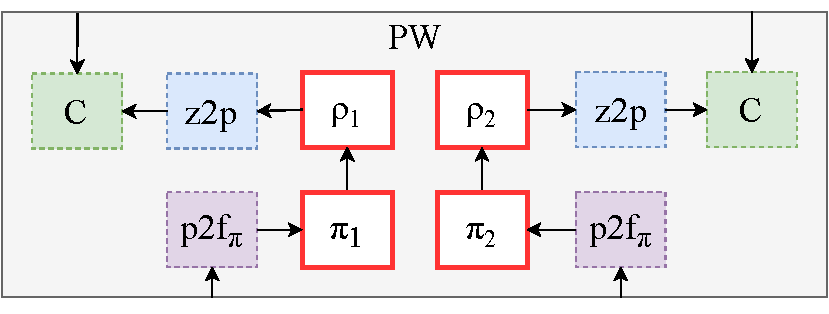
\includegraphics[scale=0.5]{figures/replacement2.pdf}
\caption{When we compose protocols we replace the \emph{p2f} process of $\rho$ with the corresponding instance of $\pi$ and its \emph{p2f} processes. By the emulation theorem, the channel offered by $\rho$ and accepted by $\pi$ have the same type.}
\label{fig:replacement}
\end{figure}

The code for the operator has the same type as any other protocol except, from the description above, it's offered channel is for the type of the functionality $\F_1$ instead of $\F_2$.
We rely on the code generation for to handle spawning instaces of a \inline{p2f} process corresponding to $\pi$ rather than $\rho$.
The operator is given in Figure~\ref{lst:compose}.
\begin{figure}
\begin{lstlisting}[basicstyle=\footnotesize\BeraMonottFamily, frame=single, mathescape]
$\tb{proc}$ compose[K][z,p]:
  (pid: Int), (rng: [Bit]), (sid: session[1]),
  (pid: Int), ($\$$z2p: z) |- ($\$$c: p) =
{
  $\$$ch <- PS.rho <- k rng sid pid $\$$z2p ;
  $\$$c <- Ps.pi <- k rng sid pid $\$$ch 
}
\end{lstlisting}
\caption{The composition operator accepts the same parameters as any other protocol party and offers the channel of type $p2f$ of the realizing protocol $\pi$. We connect $\rho$ to $\pi$ as an environment giving input to $\pi$. We do not need to include any import in our composition operator as the two protocols are guaranteed to be well-matched by the emulation definition. The operator replaces only one party (one \msf{pid}), and the \partywrapper instantiates parties that run the composed protocol.}
\label{lst:compose}
\end{figure}

The resulting composition operator, which composes the two simulators \SIM{\rho} and \SIM{\pi} inside the construction simulator, is best described in text as the resulting code is too verbose to include in the main body of this paper.
You can find the full simulator composition operator in the appendix.
\begin{itemize}
	\item Input from \Z is split between the two simulators
	\begin{itemize} 
		\item \inline{Z2A2P(pid, msg)} intended for parties of $\rho$ are passed to \SIM{\rho}
		\item \inline{Z2A2F(msg)} intended for $\F_1$ is passed to \SIM{\pi}.
	\end{itemize}
	\item Output from \SIM{\pi}: 
	\begin{itemize}
		\item \inline{A2F(msg)} for $\F_2$ and \inline{A2P(pid,msg)} for dummy parties of $\F_2$ are sent to \SIM{\rho} as \inline{Z2A2F(msg)}
		\item \inline{F2A2Z(msg)} is sent to \Z unaltered.
	\end{itemize}
	\item Output from \SIM{\rho}: 
	\begin{itemize}
		\item \inline{A2F(msg)} and \inline{A2P(pid,msg)} for $\F_3$ are sent out unaltered.
		\item \inline{F2A2Z(msg)} messages are sent to \SIM{\pi} as \inline{F2A(msg)} from $\F_2$.
		\item \inline{P2A2Z(pid,msg)} messages are sent to \Z unaltered.
	\end{itemize}
\end{itemize}
The simulator relies on simulators for $\F_1 \xrightarrow{\pi} \F_3$ and $\F_2 \xrightarrow{\rho} \F_3$ to satisfy simulation for Theorem~\ref{thm:singlecomp}.
It is clear that this construction adequately simulates the composed protocol. 
The type in the ideal world gurantees that both the real and ideal world adversaries get at least as much impor as any of the protocol parties. 
This ensures that the composed simulator has enough import to sandbox the two existing simulators and send import out to the ideal world parties and ideal funfctionality.
Therefore it is trivial to see that the composed simulator is well-resource-typed.

Another illustrative description of what composition proposes, logically, is shown by this series of UC executions where the $\equiv$ operator denotes equivalent UC executions that result from moving ITMs in and out of a sandbox, and $\approx$ indicates emulation:
\begin{align}
& \msf{execUC} \: \Z \, (\rho \circ \pi) \, \F_1 \, \DA \\
\equiv \; & \msf{execUC} \: (\Z \circ \rho) \, \pi \, \F_1 \, \DA \\
\approx \; & \msf{execUC} \: (\Z \circ \rho) \, \idealP \, \F_2 \, \SIM{\pi} \\
\equiv \; & \msf{execUC} \: \Z \, \rho \, \F_3 \, (\SIM{\pi} \circ \SIM{\rho})
%\approx \; & \msf{execUC} \: (\Z \circ \Sim{\pi}) \, \idealP \, \F_3 \, \Sim{\rho} \\
%\equiv \; & \msf{execUC} \: \Z \, \idealP \, \F_3 \, (\Sim{\pi} \circ \Sim{\rho}) 
\end{align}

%\item Inputs from \Z of \inline{Z2A2P(msg)} are passed to \SIM{\rho}, and inputs of \inline{Z2A2F(msg)} are passed to \SIM{\pi}.  
%\item \inline{P2A2Z(pid, msg)} outputs from \SIM{\rho} are forwarded to \Z unaltered.
%\item \inline{A2F(msg)} and \inline{A2P(pid, msg)} messages from \SIM{\pi} for $\F_2$ are sent to \SIM{\rho} as \inline{Z2A2F(msg)} and \inline{Z2A2P(pid, msg)}, respectively. 
%\item In the reverse direction, \inline{F2A2Z(msg)} messages from \SIM{\rho} are sent to \SIM{\pi} as \inline{F2A(msg)}, and, finally, \inline{F2A2Z(msg)} output generated by \SIM{\pi} is forwarded to \Z.
%\item \inline{A2P(pid,msg)}, \inline{A2F(msg)} messages from \SIM{\rho}, and \inline{P2A(pid,msg)} and \inline{F2A(msg)} from $\F_3$, are forwarded unaltered. 
%\end{itemize}

%We also provide a composition operator for simulators to construct a simulator for the composed protocol. We connect the simulatorsin the following way
%\begin{figure*}
%\begin{lstlisting}[basicstyle=\small\BeraMonottFamily, frame=single, mathescape]
%$\tb{proc}$ sim_compose[K][a2r,r2a][a2p,p2a][a2f,f2a]:
%  (k: Int), (rnd: [Bit]), (sid: session[1]),
%  (#z_to_a: comm[z2amsg[a2r][a2f]]), (#a_to_z: comm[a2zmsg[r2a,f2a]]),
%  (#a_to_p: comm[a2pmsg[a2r]]), (#p_to_a: comm[p2amsg[r2a]]), (#a_to_f: comm[a2fmsg[a2f]]), (#f_to_a: comm[f2amsg[f2a]])
%    |- ($\$$c: 1) =
%{
%  $\$$ch 
%\end{lstlisting}
%\end{figure*}

%\begin{figure*}
%\begin{lstlisting}[basicstyle=\small\BeraMonottFamily, frame=single,  mathescape]
%$\tb{proc}$ compose[K][z2r][r2z][f2r][r2f][p2f][f2p] : 
%    (pid: Int), ($\$$z_to_p: c[K][z2p]), ($\$$p_to_z: c[K][r2z]), 
%    ($\$$f_to_p: c[K][f2r]), ($\$$p_to_f: c[K][r2f])  |- ($\$$D : 1) =
%{
%	$\$$rho_to_pi <- $\tm{createchan}$[K][p2f];
%	$\$$pi_to_rho <- $\tm{createchan}$[K][f2p];
%
%	 <- pi  <-                 $\$$rho_to_pi $\$$pi_to_rho $\$$p_to_f $\$$f_to_p ;
%	 <- phi <- $\$$z_to_p $\$$p_to_z $\$$rho_to_pi $\$$pi_to_rho ; 
%}
%\end{lstlisting}
%\caption{Composition operator in Nomos that connects a protocol $\rho$ to a protocol $\pi$ that uses some functionality $\F$. The operators creates new channels to connect the realizing $\pi$ and it's hybrid \F. Output from $\rho$ intended for the replace functionality are actually send to parties of $\rho$, and channels outgoing from the parties to the functionality are given to $\pi$.}
%\label{lst:compose} 
%\end{figure*}

%\begin{theorem}[Composition]\label{thm:singlecomp}
%\begin{mathpar}
%\inferrule*[right=single-compose]
%{
%	\F_1 \xrightarrow{\pi} \F_2 \semi \F_2 \xrightarrow{\rho} \F_3 \\
%}
%{
%	\F_1 \xrightarrow{\rho \circ \pi} \F_3
%}
%\end{mathpar}
%
%If \textit{well-typed} $(\pi, \F_1$) realizes $\F_2$ and ($\rho$, $\F_2$) realizes some $\F_3$, then $(\rho \circ \pi, \F_2)$ is \textit{well-typed} and realizes $\F_3$ when $\circ$ is defined as in Figure~\ref{lst:compose}.
%\end{theorem}

%\begin{proof}
%The pre-condition ensures the existence of \textit{well-resource-typed} simulators $\Sim_\rho$ for $\F_2 \xrightarrow{\rho} \F_3$ and $\Sim_\pi$ for $\F_1 \xrightarrow{\pi} \F_2$, and, it is obvious that the composed protocol is also well-resource-typed.
%We construct a simulator \Sim' for the dummy adversary to show
%\[
%	\msf{execUC}\ (\rho \circ \pi)\ \F_1\ \Z\ \A \approx \msf{execUC}\ \idealP\ \F_3\ \Z\ \Sim''
%\]	
%
%The simulator $\Sim'$ relies only simulating \SIM{\pi} and \SIM{\rho}.
%Note that \SIM{\pi} can accept messages for $\pi$ or $\F_1$, simulate them, and generate input for $\F_2$. 
%Similarly, \SIM{\rho} can take inputs for $\rho$ or $\F_2$, simulate them, and generate input for $\F_3$.
%Therefore, we connect the two simulators in the natural way:
%\begin{itemize}
%\item Inputs from \Z of \inline{Z2A2P(msg)} are passed to \SIM{\rho}, and inputs of \inline{Z2A2F(msg)} are passed to \SIM{\pi}.  
%\item \inline{P2A2Z(pid, msg)} outputs from \SIM{\rho} are forwarded to \Z unaltered.
%\item \inline{A2F(msg)} and \inline{A2P(pid, msg)} messages from \SIM{\pi} for $\F_2$ are sent to \SIM{\rho} as \inline{Z2A2F(msg)} and \inline{Z2A2P(pid, msg)}, respectively. 
%\item In the reverse direction, \inline{F2A2Z(msg)} messages from \SIM{\rho} are sent to \SIM{\pi} as \inline{F2A(msg)}, and, finally, \inline{F2A2Z(msg)} output generated by \SIM{\pi} is forwarded to \Z.
%\item \inline{A2P(pid,msg)}, \inline{A2F(msg)} messages from \SIM{\rho}, and \inline{P2A(pid,msg)} and \inline{F2A(msg)} from $\F_3$, are forwarded unaltered. 
%\end{itemize}
%It is clear that \Sim' is able to emulate inputs from \Z to both parties of $\rho$ and the ideal functionalty $\F_1$.
%\Sim' performs constant over head in simulating two \emph{well-resource-typed}, and therefore it is clear that \Sim' is \emph{well-resource-typed}.
%When combined with the \emph{dummy lemma}, a well-resource-typed simulator exists for composition for any adverasry \A. 
%The dummy lemma presented above ensures that a simulator for any \A can be constructed that is well-resource-typed for all wel-resource-typed \A.
%\end{proof}
%
%We give a simpler, high-level idea of the forst step of the proof proof here which can be understood visually:
%The $\equiv$ operator is a result of moving around ITMs (some from within other ITMs into the main UC execution) and $\sim$ refers to indistinguishability.
%In line (13) above, $\rho$ is moved into the execution environment with an unchanged simulator as no additional simulation is required: the simulator allows unfettered communication between parties of $\rho$ and \Z.

\subsection{Multisession}

\begin{theorem}[Composition]\label{thm:composition}
\begin{mathpar}
\inferrule*[right=compose]
{
	%(\pi, !\F_1) \sim (\idealP, F_2) \semi (\rho, !\F_2) \sim (\idealP, \F_3) \\ 
	!\F_1 \xrightarrow{\pi} \F_2 \semi !\F_2 \xrightarrow{\rho} \F_3 \\
	%\Rightarrow \exists \Sim(\A) \vdash (\rho^{!\F_2 \rightarrow (!\pi \, \circ \, \msf{squash})}, !\F_1) \sim (\idealP, \F_3)
}
{
	!\F_1 \xrightarrow{\rho \, \circ !\pi \circ \, \msf{squash}} \F_3
	%(\rho \, \circ \, !\pi \circ \msf{squash}, !\F_1) \sim (\idealP, \F_3)
}
\end{mathpar}
\end{theorem}
Full composition in the UC framework extends beyond the simpler composition in Theorem~\ref{thm:singlecomp} which only defines replacement of one functionality with a protocol that realizes it.
Instead, UC composition allows for replacement of any number of instances of a functionality with instancesof the realizing protocol.
Theorem~\ref{thm:composition} illustrates the full composition theorem using our arrow notation, and highlights a theorem that we must prove before we can achieve full composition.
It relies on Theorem~\ref{thm:squash} that introduces the \msf{squash} protocol and the $!$ operator.
Notice that Theorem~\ref{thm:compose} follows directly from Theorem~\ref{thm:singlecomp} and Theorem~\ref{thm:squash}.

The multi-session extension of a protocol or functionality, specified by the $!$ operator (such as $!\rho$ or $!\F$), allows multiple instances of the protocol/functionality to be run within a sinlge ITM.
An ITM simulates the instances and multiplexes input/output to/from them much like the \partywrapper.

\begin{theorem}[Squash Theorem]\label{thm:squash}
%If a functionality \F is well-resource-typed, then $!\F$ and $!!\F$ are well-resource-typed (by Theorem~\ref{thm:bangppt}) and $(\idealP, !!\F) \sim (\msf{squash}, !\F)$.
%\textit{Well-resource-typed} \F $\Rightarrow$ $!\F \xrightarrow{\msf{squash}} !!\F$%  $(\idealP, !!\F) \sim (\msf{squash}, !\F)$
\begin{mathpar}
\inferrule*[right=squash]
{
\textit{well-resource-typed} \; \F
}
{
!\F \xrightarrow{\msf{squash}} !!\F
}
\end{mathpar}
\end{theorem}

For the multisession extension of a fuctionality, the type is straightforward and ony acts to multiplex input/outpt based on the intended target \inline{ssid}.
\begin{center}
\parbox{0cm}{
\begin{tabbing}
$\m{{P2MS}[a,b]\{n,m\}} = \textcolor{red}{\getpot^n} \ichoice{\mb{Inp}: ssid \arrow a \tensor \echoice{$\=$\mb{Ok}: \textcolor{red}{\paypot^0} \; \m{P2MS[a,b]\{n,m\}},$ \\
\>$\mb{Out}: ssid \arrow b \tensor \textcolor{red}{\paypot^m} \; \m{P2MS[a,b]\{m,n\}}}}$
%\m{MS2P[a][b]\{n,m\}}}$ \\
%\mi{stype} \; \m{{MS2P}[a][b]\{n,m\}} = \echoice{\mb{Ok}: \textcolor{red}{\paypot^0} \; \m{P2MS[a][b]\{n,m\}}, \mb{Out}: ssid \product b \arrow \textcolor{red}{\paypot^m} \; \m{P2MS[a][b]\{n,m\}}}  
\end{tabbing}}
\end{center}
The multisession extension is mentioned in greater detail in the appendix.
%and the functional types that are sent to the wrapper surrounding it are given by
%\begin{lstlisting}[basicstyle=\small\BeraMonottFamily, mathescape]
%$\yo{type}$ p2ms[a] = P2MS of ssid ^ a ;
%$\yo{type}$ ms2p[b] = MS2P of ssid ^ b ;
%\end{lstlisting}
%It is important to note that we require a session type here instead of allowing !\F act as the functionality wrapper because, when composed it must communicate directly communicate, over a session-typed channel, to another protocol.
%Furthermore, the construction of !\F is the same as in the \Fro example: one session typed channel for all parties.
%In Figure~\ref{fig:multisession} illustrated the functionality wrapper (right) and the multisession extension (left) for \Fcom. 
%\begin{figure}
%\centering
%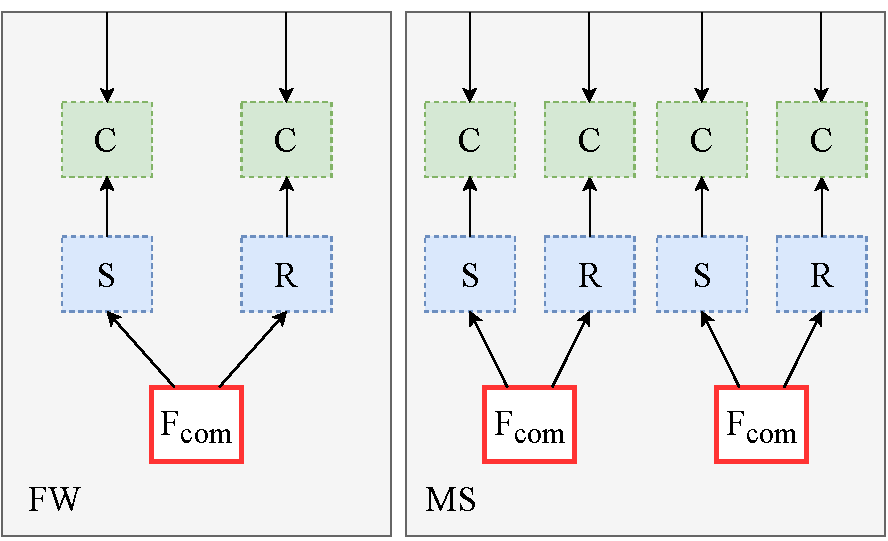
\includegraphics[scale=0.5]{figures/multisession.pdf}
%\caption{The multisession extension of \Fcom (right) with only two instances, creates the same processes $S$ and $R$ (offering the session typed channel to \Fcom) for every created instance. A communicator per session buffers messages for the $S$ and $R$ processes to consume and forward along their session-typed channel to \Fcom.}
%\label{fig:multisession}
%\end{figure}

%As a generic construction provided by NomosUC, the multisession operator requires some code generation but only to accept an arbitrary number of virtual token types if the underlying \F simulators other processes. 
%Furthermore, similar to the functionality wrapper, the multisession operator constructs the processes around \F in the same way and spawns them on-demand.
%The process definition for $!\F_\msf{com}$ is shown in Figure \ref{lst:bangf} accepting two token types: the real token type $K$ and the virtual token type $K_1$ for instances of $\F_\msf{com}$.
%
%\begin{figure}
%\begin{lstlisting}[basicstyle=\footnotesize\BeraMonottFamily, frame=single, mathescape]
%$\tb{proc}$ bangF[K,K1][p2f,...] :
%  (k: $\tgr{Int}$), (rng: [Bit]), (sid: session[a]), 
%  ($\$$p: P2MS[p2f][f2p]) |- ($\$$ch: 1) =
%\end{lstlisting}
%\caption{The type definition for the multisession operator for functionalities and the correspond message type and import parameters. The operator for protocol parties is identical in code but differens in that the parameters to the \texttt{P2MS} type are for \texttt{Z2P} interaction.}
%\label{lst:bangf}
%\end{figure}

\begin{theorem}[PPT !]\label{thm:bangppt}
If a functionality $\F$ is well-resource-typed, then it's multisession extension $!\F$ is well-resource-typed.
\end{theorem}

We examine this theorem in greater detail in the appendix. 
At a high-level it is obvious that such a construction, activated polynomially many times, is well-resource-typed as long as the underlying functionality/protocol is well-resource-typed.
%\begin{proof}
%A \textit{well-resource-typed} \F guarantees a polynomial $T_{\F}$ bounding its execution.
%In the worse-case, the multisession operator must spawn a new instance of $\F$ an every activation. 
%Let $N_{\F}$ denote the total number of instances (and, hence, number of activations) of $\F$ created by the operator.
%Note that $N_{\F}$ is polynomial in the security parameter $k$ for all well-typed environments, protocols, and adversary.
%Therefore, there always exists a bounding polynomial to bound a polynomial number of simulated instances of \F.
%The polynomial can be given as:
%$$ P_{!\F}(n) = N_{\F} P_{\F}(n) + \mathcal{O}(N_{\F}) $$
%where the $\mathcal{O}(N_{\F})$ is due to the overhead of maintaining and accessing the set of all instances.
%
%Similarly, \F being \textit{well-resource-typed} ensures a valid token context for all processes it may simulate. 
%Therefore, it is clear that there exists a global connecting poltnomial $f$ that ensures a valid token context for $!\F$.
%\end{proof}


%\begin{figure}
%\begin{lstlisting}[basicstyle=\small\BeraMonottFamily, mathescape, frame=single]
%$\yo{type}$ p2bFmsg[a] = P2bF of ssid ^ a ;
%$\yo{type}$ p2bbFmsg[a] = P2bbF of ssid ^ ssid ^ a ;
%$\tg{(* z2p : comm[z2pmsg[p2bbf[a]]] *)}$
%$\tg{(* p2f : comm[p2fmsg[P2bf[a]]] *)}$
%pid = recv $\$$z2p ;
%m = recv $\$$z2p ;
%case m (
%  P2bbF(ssid1, ssid2, m) =>
%    send $\$$p2f P2bF(ssid1 + ssid2, m) ;
%)
%\end{lstlisting}
%\caption{The \textit{squash protocol} accepts a message intended intended for $!!\F$ of type \inline{P2MS[p2ms[a]][ms2p[b]]}, i.e. of the form $(\msf{ssid}_1, (\msf{ssid}_1, msg))$.
%It ``flattens'' it into a single $\msf{ssid}_3 = \msf{ssid}_1 + \msf{ssid}_2$ that can be passed to $!\F$. The result is the same number of instances of \F but behind only a single $!$ operator.}
%\label{fig:squash}
%\end{figure}

\begin{proof} (Theorem~\ref{thm:squash})
On examination the \msf{squash} theorem does constant work per activation and concantenates two \inline{ssid}s into one for messages going to the functionality and does the inverse for messages incoming from the functionality.
We provide more detail for a proof of Theorem~\ref{thm:squash} in the Appendix, however, it is clear to see that the this theorem holds with a trivial simulator.
%First we describe the \msf{squash} protocol where $!!\F$ are nested $!$ operators.
%The protocol accepts messages intended for $!!\F$ of type \inline{P2MS[p2ms[a]][ms2p[b]]}, i.e. of the form $(\msf{ssid}_1, (\msf{ssid}_2, msg))$, and ``flattens'' them into a single message of type $\inline{P2MS[a][b]}$, i.e. of the form $(\msf{ssid}_3, msg)$.
%
%In $(\idealP, !!\F)$, \idealP~expects to receive messages of the form $(\msf{ssid}_1, (\msf{ssid}_2, m))$ where $\msf{ssid_2}$ is a sub-session of $\F$ (i.e. instance) inside some $!\F$ with sub-session id $\msf{ssid}_1$ inside of $!!\F$ (the message accesses functionality $\F[\msf{ssid}_1][\msf{ssid}_2]$).
%The \msf{squash} protocol flattens the indexing of instances of \F and combines session ids $\msf{ssid}_1$ and $\msf{ssid}_2$ into a single \msf{ssid}: $\msf{ssid}_3 := \msf{ssid}_1 \cdot \msf{ssid}_2$.
%If follows intuitively that the view for the environment remains the same. 
%
%We construct a simulator such that:
%\[
%\msf{execUC} \, \Z \, \idealP \, !!\F \, \SIM{\msf{squash}} \approx \msf{execUC} \, \Z \, \msf{squash} \, !\F \DA 
%\]
%The simulator is very simple. 
%Inputs to/from parties/\Z for a corrupt party is forwarded unmodified.
%Input intended for $!\F$ of the form $(\msf{ssid}_1 \cdot \msf{ssid}_2, msg)$ is sent as $(\msf{ssid}_1, (\msf{ssid}_2, msg))$ to $!!\F$. 
%Output from $!!\F$ is modified inversely and sent to \Z.
%
%The proposed simulator is trivially analyzed to be \textit{well-resource-typed}.
%It performs constant work per activation and does ``real'' simulation other than message modification to/from $!!\F$.
\end{proof}

\subsection{UC Composition}
Finally, we can conlude with full composition in Theorem~\ref{thm:compose}.
The proof follows directly from Theorems~\ref{thm:singlecomp} and \ref{thm:squash}.

\begin{proof}
By Theorem~\ref{thm:singlecomp} we can construct a simulator \SIM{1} for $!!\F_1 \xrightarrow{\rho \, \circ \, !\pi} \F_3$.
Theorem~\ref{thm:squash} then allows us to ``squash'' $!!\F_1$ and construct a simulator using \SIM{1} for $!\F_1 \xrightarrow{\rho \, \circ \, !\pi \, \circ \, \msf{squash}} \F_3$
\end{proof}

\subsection{Design Discussion}
One of the core research questions that this work aims to study session types applied to the UC framework. 
In this section, we discuss how resource-aware session types impact the design of functionalities in NomosUC as well as which are implementable.
We use the two-way authenticated channel functionality \Fauth to througout this discussion.

In plain session types, communication between two parties $P_s$ and $P_r$ occurs over a single duplex channel.
In UC the role of the adversary as a message scheduler in \Fauth, the most common network channel model, means a more complicated functionaty involving $P_s$, $P_r$, \F, and \A. 
The simplest, and most common approach, to \Fauth is the following communication pattern: a party $P_s$ sends a message to \Fauth, \Fauth sends the message to \A and waits for \A to say \inline{OK} before delivering the message to $P_r$.
Since both parties can send a message and receive a message, it is unclear which process, \Fauth or $P$, will be active along that channel at any given time.
Session types require this information to be statically known when two processes are communicating over a single channel--making this communication pattern unexpressable over a single channel.

There a few ways to overcome this constraint. 
In general, even though the UC framework places few restructions of communication patterns, most functionalities stick to a few.
\Fauth, for example, can take a few forms:
\begin{enumerate}
\item (presented above) Receiver and adverasry are activated directly: \Fauth waits for \A to tell it to deliver the message.
\item \Fauth ``polling'' approach: messages from $P_s$ are buffered for both \A and $P_r$. \A and $P_r$ must ask \Fauth for new messages. This is a more invonconvenient method, but can be useful for novel functionality designs that need a channel.
\item ``polling'' but receiver is activated: the message is stored in a buffer for \A, and \A's deliver message directly sends it to $P_r$.
\end{enumerate}
The simplest way to implement \Fauth in NomosUC is ``polling'' approach. As far as we know, we can systematically tranform any UC functionality into one that uses ``polling''. 
The consequences are that polling is inconvenient from a programming point of view because \Z needs to continuously activate parties to ask for new messages.
Hope is not lost though, because it turns out our type system can express functionalities in all three of the ways listed above. 
The first, and most natural, approach only requires splitting communicating between $P$ and \Fauth into two unidirectional channels
Such an extension to NomosUC trivially modifies the \partywrapper to handle two channels instead of one, and the types of the channels can be succintly expressed as: 
\begin{center}
\parbox{0cm}{
\begin{tabbing}
$\m{sending}[a] = \textcolor{red}{\getpot^n} \ichoice{\mb{sendmsg}: \m{a} \tensor \m{sendmsg}}$ \\
$\m{receive}[a] = \textcolor{red}{\getpot^m} \echoice{\mb{recv}: \m{a} \tensor \m{receive}}$ \\
$\m{adv}[a] = \echoice{\mb{leakmsg}: a \tensor \ichoice{ \mb{ok}: \m{leakmsg}}}$
\end{tabbing}}
\end{center}
The first to correspond to the channels for sending from $P$ to \Fauth and the second in the opposite direction. The third is the adversary's channel at \Fauth.

A notable part of our contruction is the machinery created around the protocol parties and functionality that intemediate their communication with communicators and functionally-typed messages.
Recall that such compromises are required in order to allow a \emph{dynamic} number of parties in UC.
The session type of the shared channel of a communicator only allows for a fixed amount of import to be sent over it with every messages. 
Protocols and functionalities that send different amounts of import depending on the message, say $i_1,...,i_n$, must now send $\m{max}(\{i_j\})$ import with every messages.
For existing UC definitions this appears to be an issue of ensuring a machine has \emph{enough} import, however, we can systematically map any UC import definition to one that works in NomosUC~\footnote{The problem can be reduced to ensuring enough ``latent'' import needed to compute, and, because we aren't concerned here with \emph{tight} computational bounds the problem is quite easy to solve. We discuss in greater detail in the appendix.}.




%\section{flip}
%In this section we introduce a coin flip functionality \Fflip and discuss how composition affects its import requirements, and we introduce a design pattern where session types can enforce message ordering across multiple channels. 
\Fflip is realized by protocol $\prot{flip}$ in the $\F_{\msf{comauth}}$-hybrid world (a functionality combining \Fcom with a one-way, one-shot channel, \Fauth, from the receiver to the sender). 
In this section we again go through assigning consatnt import but this time notice how import assignments change when, say, a functionality is used by different protocols. 
%We push the realizing protocols, simulators, and process code to Appendix~\ref{app:flip} and focus here on the \Fflip and \Fropp session types.

\begin{figure*}
	\begin{center}
	\parbox{0cm}{
	\begin{tabbing}
		$\m{flip[K]\{n\}\{m\}} = \ichoice{\mb{init}: \rpaypot{n} \; K \arrow \ichoice{\mb{getflip}: \rpaypot{n}  \echoice{ $\=$\mb{yes}: \rgetpot{m} \; Bit \product 1,$ 
		$ \mb{no}: \rgetpot{m} \; \m{flipped}[K]}}}$ \\
		$\m{receiver[K]\{n\}\{m\}} = \ichoice{\mb{getflip}: \rpaypot{n} \; \echoice{$\=$ \mb{yes}: \rgetpot{m} \; Bit \product 1,$
		$\mb{no}: \rpaypot{m} \; \m{receiver[K]}}}$ \\
		$\m{adv[K]\{n\}} = \echoice{\mb{askflip}: \; K \arrow \echoice{\mb{flipok}: \ichoice{$\=$\mb{yes}: 1,$
		$\mb{no}: 1}}}$
	\end{tabbing}}
	\end{center}
	\vspace{-5mm}
	\caption{The session types describing \Fflip's channels with the flipper, receiver, and the adversary.}
	\label{fig:fliptype}
\end{figure*}

The code for \Fflip is quite simple and shown below and the types \inline{flipper} and \inline{receiver} shown in Figure~\ref{fig:fliptype}.
\begin{lstlisting}[basicstyle=\scriptsize\BeraMonottFamily, frame=single, mathescape]
$\nproc$ F_coinflip[K]{p2fn}{m} :
  (k: Int), (rng: [Bit]), (sid: session[1]),
  ($\$$F: flipper[$\tp{K}$]{$\tp{p2fn}$}{$\tp{f2pn}$}), ($\$$R: receiver[$\tp{K}$]{$\tp{p2fn}$}{$\tp{f2pn}$}),
  ($\$$A: adv[$\tp{K}$]) |- ($\$$c: 1) =
{
  $\ncase$ $\$$F (
    init =>
      x = $\nrecv$ $\$$F ;
      $\nget$ $\$$F {p2fn}
      b = sample 1 rng ;
      $\$$A.flipped ;
      $\nsend$ $\$$A x ;
      $\tg{(* wait for getflips *)}$
      $\$$f <- getflip_f{$\tp{p2fn}$}{$\tp{f2pn}$} <- b $\$$F ;
      $\$$r <- getflip_r[$\tp{K}$]{$\tp{p2fn}$}{$\tp{f2pn}$} <- b x $\$$R ;
  )
}

$\nproc$ getflip_f[K]{p2fn}{m} :
  (k: Int), (rng: [Bit]), (sid: session[s]),
  (b: Bit), ($\$$F: f_flipped[$\tp{K}$]{$\tp{p2fn}$}{$\tp{f2pn}$}),
  ($\$$A: adv[$\tp{K}$]) |- ($\$$c: 1) =
{
  $\ncase$ $\$$F (
    getflip =>
      $\$$A.askflip ;
      $\ncase$ $\$$A (
        yes => 
          $\$$F.yes ; $\nsend$ $\$$F b ;
          $\npay$ {f2pn} K $\$$F ;
        no => $\$$F.no ; $\npay$ {f2pn} K $\$$F ;
      )
  )
}
\end{lstlisting}
The code for  \inline{getflip_r} is identical except it is the receiver. 
It checks for a flip result by either party, \Fflip asks the adversary whether to deliver the output to the party asking for it.
Much like the real-world case where if the corrupt committer never opens its commitment, the simulator here can ensure that only the flipper receives the flip.
As the session type indicates, the adversary responds with a \inline{yes} or \inline{no} to deliver the flip.

\subsection{Protocol for Flipping}
The protocol we use to realize the coin flip uses \Fcom, used throughout this work, and a one-way channel $\F_{\msf{auth}}$ which allows messages to be sent in both directions. 
Its type differs from \Fcom alone.
Again we split communication between two uni-direction channels for each of the committer and receiver unlike \Fcom.
The types of the channels are
\begin{center}
\parbox{0cm}{
\begin{tabbing}
	$\m{commitp2f}[a]\{m\} = $\\
	\qquad $\ichoice{$\=$\mb{commit}: \rpaypot{2} Bit \product \m{committedp2f}[a]}$ \\
    	%\>$\mb{sendmsg}: \rpaypot{m} a \product \m{commitp2f}[a]}$ \\
	$\m{committedp2f}[a]\{m\} = $\\
	\qquad $\ichoice{$\=$\mb{open}: \m{donep2f}[a]}$ \\
		%\>$\mb{sendmsg}: \rpaypot{m} a \product \m{committedp2f}[a]}$ \\
	$\m{commitf2p}[a] = \echoice{\mb{msg}: \rgetpot{m} a \arrow \m{commitf2p}[a]}$ \\
	$\m{receivep2f}[a] = \ichoice{\mb{sendmsg}: \rpaypot{m} a \product \m{receivep2f}[a]}$ \\
	$\m{receivef2p}[a] = \echoice{$\=$\mb{committed}: \m{receivedf2p}[a]}$\\
		%\>$\mb{msg}: \rgetpot{m} a \arrow \m{receiverf2p}[a]}$ \\
	$\m{receivedf2p}[a] = \echoice{$\=$\mb{opened}: Bit \arrow \m{donef2p}[a]}$ \\
	    %\>$\mb{msg}: \rgetpot{m} a \arrow \m{receivedf2p}[a]}$ \\
\end{tabbing}}
\end{center}
Again, this type is seen by wrapped instances of \prot{flip} and, as far as the commitment inputs, is the same type that \Fcom sees (we use different names here to distinguish channels). 

%Notice that the ordering of messages locally for the committer and receiver are still present. 
Notice that the inputs for the committer have not changed, and it additionally has a channel to receive messages from the channel functionality. 
Like the example of $\pi_\msf{com}$ above, we can set the parameters as necessary for $\prot{flip}$.
As you'd expect the commitment functionality takes in some amount of non-zero import, here it's 2 for the random oracle assumption we're working with, to ensure that it's able to perform some polynomial amount of work in computing hashes, 
and that the \mb{sendmsg} branches take an arbitrary amount of import allowing a sender to send $m$ import to the other party. 

The protocol that realizes this functionality, $\pi_{\msf{commauth}}$ is identical to $\pi_{\msf{com}}$ except it forwards $\mb{sendmsg}$ messages to the hybrid functionality \Fropp' that allows for \emph{2-way} communication, that is one-shot in each direction, rather than the original one-way channel. 
Notice that \Fropp' has a two-way channel, because $\pi_{\msf{commauth}}$ will send messages from committer to receiver and vice versa, but the high level $\F_{\msf{commauth}}$ only exposes the new feature of sending messages from the receiver to the committer. 
Getting to the two-way channel from \Fropp only requires the following on top of the session type in Figure~\ref{fig:fropptype}: 
\begin{itemize}
	\item an additional $\mb{sendmsg}$ on \m{rquery} that allows sending 1 import to the committer
	\item and \mb{msg} session in \m{shash} with 1 import token to let the committe receive messages.
\end{itemize}

Again we aim to set the constant amount of import that is sent through \partywrapper with \Z and \F. 
Like the original commitment, the \partywrapper, running wrapped instances of \prot{flip}, needs sends 4 units of import to $\F_{\msf{commauth}}$ on \mb{commit}, \mb{open}, and \mb{sendmsg} inputs due to the protocl that we are using. 
Additionally, the one-way message carrying the randomness $r$ from the receiver to the comitter which, by virtue of the 4 import for the commitment, must result in the \partywrapper sending 4 import to $\F_{\msf{commchan}}$.

Given these import requirements, we can assign a sufficient assignment of import that the \partywrapper receives from \Z. 
We conclude that a constant of 12 import per input from \Z is sufficient to accomdate all $\F_{\msf{commchan}}$ inputs including the message sent from the receiver. 

We elide similar reasoning and assignment for communication betwen the \partywrapper and \A because it is much simpler, however it is clear to see that it is easy to determine such assignments and conclude that the providerless channels construction, import-wise, does not conflict with the generalized composition operator.
All the import assigned here, both for the sessio types seen by the wrapped protocol parties and the constant amounts sent to/from the \partywrapper, are checked and validated by the NomosUC type system. 

%\subsection{Simulator}
%The protocol for the coin flip uses \Fcom. 
%The flipper commits to a bit $b$, the receiver sends the flipper a random bit $r$ in return, the flipper opens its commitment, and both parties compute the flip as $r \oplus b$.
%The simulator for this protocol to realize \Fflip is straightforward:
%\begin{itemize}
%\item If the flipper is corrupt, the simulator tells the flipper to \inline{init} the flip when the environment sends it a \inline{Commit b} message. It gets the flip outcome $f$ from the flipper and simulates the receivers random bit $r = f \oplus b$ for the environment. It never delivers the flip outcome to the receiver unless the environment instructs it to open the flipper's commitment. By setting $r = f \oplus b$, when the environment receives $f$ it can check that $r \oplus b = f$.
%\item If the receiver is corrupt, the simulator waits for \Fflip to inform it that the flip was initiated. It simulates the \inline{Commit} message from \Fcom to the receiver, for \Z. When it receives the random bit that \Z wants the receiver to send, it gets the flip outcome from the receiver, computes $b = r \oplus f$ and sends \inline{Open b} to \Z. Again, \Z can verify $b \oplus r$ similar to the above case.
%nl
%\end{itemize}
%
%\subsection{Composition}
%We describe a composition theorem in the previous section, a composition operator for protocols, and a brief highlight of the composition operator for simulators.
%Composition of the coin flip with the commitment protocol is realized with simulator composition in exactly this way.
%We give a diagram of simulator composition in~\ref{fig:simcomp}.
%\begin{figure}
%\centering
%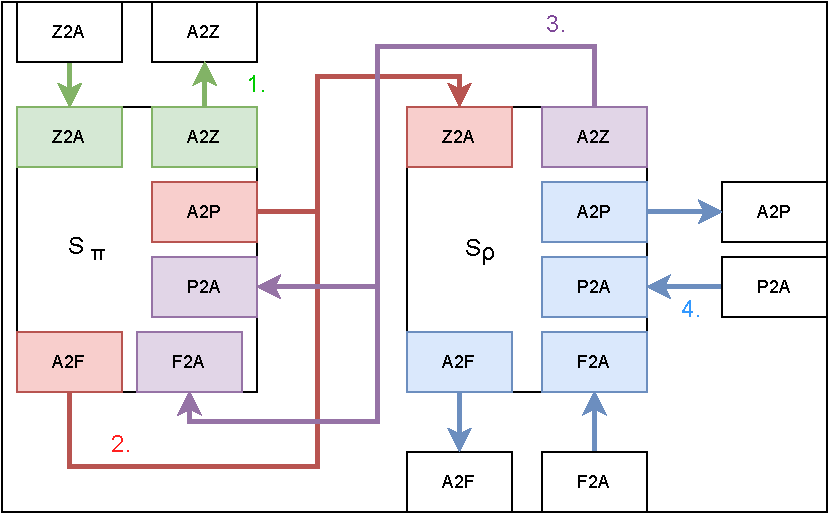
\includegraphics[scale=0.5]{figures/simcomp.pdf}
%\caption{The composed simulators for $\F_1 \xrightarrow{\rho \circ \pi} \F_3$. The real world consists of $(\rho \circ \pi, \F_1)$. Inputs from \Z are for $\F_1$ and dummy parties interacting with $\F_1$, which \SIM{\pi} is equipped to handle. Outputs from \SIM{\pi} are for $\F_2$ and dummy parties of $\F_2$ which \SIM{\rho} is equipped to handle. Finally, outputs from \SIM{\rho} are for $\F_3$ and dummy parties of $\F_3$, which is just the ideal world in Theorem~\ref{thm:composition}.}
%\label{fig:simcomp}
%\end{figure}


%\section{Ideal Functionalities} \label{sec:idealfs}
%In this section we explore some of the tradeoffs introduced earlier and the design space for ideal functionalities in NomosUC.
Specifically, we explore the polymorphism described in Section~\ref{sec:execuc} that mitigates the loss of expressiveness of session types that arises from splitting communication, between a party and a functionality, into two uni-directional channels.
We also share two functionalities, the random oracle \Fro as an example of a type that allows dynamic parties with only one channel, and we compare secure message communicatin (\Fsmc, a simpler version of \Fauth) to writing functionalities in a closely related work: easyUC~\cite{easyuc}.

\subsection{Polymorphism for Ideal Functionalities}
We mention in the previous section that despite splitting communication for \Fauth into two uni-directional channels per party, we use polymorphism to achieve message ordering between channels as well.
A contrived example of such a type below shows that with minimal extra variables in a type can achieve the same for arbitrarily complicated functionalities. 
The idea is that we can add an arbitrary number of variables to achieve the desired oredering by allowing the protocol to determine the concrete types for each type parameter. 
The tradeoff is extra session type clutter, from including multiple type variables that don't carry any data, but as we see with the type and functionality definition below the type is still clear upon inspection.

Imagine an ideal functionality where two parties take one of two roles with the following session types:
\begin{center}
	\parbox{0cm}{
	\begin{tabbing}
		$\m{role1\_p2f}[a] = \ichoice{\mb{do1}: \m{Int} \product \m{a} \product \m{role1\_p2f}}$ \\
		$\m{role1\_f2p}[a] = \echoice{\mb{do2}: \m{String} \arrow \m{a} \arrow 1}$ \\
		$\m{role2\_p2f}[a][b][c] = \ichoice{$\=$\mb{do3}: \m{a} \product \m{b} \product \m{role2\_p2f}$ \\
		\>$\mb{do4}: \m{Int} \product \m{c} \product \m{role2\_p2f}}$ \\
		$\m{role2\_f2p}[b][c] = \echoice{\mb{do5}: \arrow \m{b} \arrow \m{c} \arrow 1}$
	\end{tabbing}}
\end{center}
The session types define party 1 as giving 1 input \mb{do1} and party 2 giving two inputs \mb{do2}. 
When used with the following type definition for the a functionality
\begin{lstlisting}[basicstyle=\scriptsize\BeraMonottFamily, frame=single, mathescape]
$\nproc$ F[a, b, c]: $\tg{...}$
  ($\$$P12F: role1_p2f[a]), ($\$$F2P1: role1_f2p[a]), 
  ($\$$P22F: role2_p2f[a,b,c]), ($\$$F2P2: role2_f2p[b,c]) $\tg{...}$
\end{lstlisting}
we can achieve the following ordering of messages \emph{between} the multiple sessions:
\begin{itemize}
	\item Party 1 must give input \mb{do1} and determine the type \m{a} before \F can output \mb{do2} of that same type.
	\item Party 2 must give input \mb{do3} after party 1 gives \mb{do1}, and it must give inputs \mb{do3}, \mb{do4} (concretizing the types of \m{b} and \m{c}) before \F can output \mb{do5}.   
\end{itemize}

Functionalities whose code attempts to send concrete types over the sessions will fail to type check, and protocols that wish to realize them must also follow the same communication pattern
It is important to note here that the session type isn't enough to enforce order, but the functionality's type definition must also enforce the dependency.

\subsection{Secure Message Communication, \Fsmc}
Secure message communication, or \Fsmc, is the \Fauth functionality reduced to handle one-way communication only.
Therefore, unlike \Fauth the session type can be captured by a single channel for each party. 
The session types for \Fsmc are
{\centering
\parbox{0cm}{
\begin{tabbing}
$\m{sender}[a] = \ichoice{\mb{sendmsg}: PID \product a \product 1}$ \\
$\m{receiver}[a] = \echoice{\mb{recv}: PID \arrow a \arrow 1}$ 
\end{tabbing}}
}
The session type, in a sense, defines a state machine that is enforced by the type system.
The same functionality in a related work, EasyUC, only defines messages and function types, and requires the user code to define a state machine, perform runtime checks on inputs, reject inputs out of order, and manage communication through the EasyUC's addressing scheme. 
When compared to the entire code for \Fsmc below, the EasyUC code is at least three times as long.
Not only does that make UC definitions more complicated by introduces the potential for bugs in what should be a simple functionality\footnote{The full code of the EasyUC SMC example can be found at \url{https://github.com/easyuc/EasyUC/blob/master/smc/SMC.ec}}.
\begin{lstlisting}[basicstyle=\scriptsize\BeraMonottFamily, frame=single, mathescape]
$\nproc$ f_smc[K][a] : ($\$$S: sender[a]), ($\$$R: receiver[a]), 
	($\$$A: adv[a]) |- ($\$$ch: 1) = {
  let pidS :: PID, pidR :: PID = sid ;
  case $\$$S (
    sendmsg => pid = recv $\$$S ; m = recv $\$$S ;
               if pid == pidS then
                 $\$$A.leakmsg ; send $\$$A m ;
                 case $\$$A ( deliver => $\$$R.recvmsg ;
                              send $\$$R m ;
                 )
               else error "bad sender " ++ pid )
}
\end{lstlisting}
\todo{@andrew: i hesitate with this section because we can't afford to include code for \Fsmc in EasyUC because of space constraints so the point is slightly lost aside from my claims below but there is a URL}

We also note that we can realize \Fauth by applying the multisession operator to \Fsmc ($!\Fsmc$) and remove the need for splitting communication between two channels like we did in Section~\ref{sec:execuc}.
In general, it is better to write ideal functionalities to be as small and single-purpose as possible and combine them with generic operators, like $!$, to create more complex functionalities. 

%\subsection{Append-only Database}
%Prior notions of polynomial time in the UC framework require that ITMs execute in time polynomial in the length of their input.
%Other notions of polynomial time suggested in prior versions of the UC framework and other such notions~\ref{hofheinz} also run into problems when realizing functionalities where protocol parties 

%\section{Coin Flipping and Commitment} \label{sec:commitment}
%In this section we work throgh the entire commitment example that has seen used throughout this paper, and we show composition by realizing a coin flipping ideal functionality \Fflip and a protocol realizing it in the \Fcom-hybrid world.
We present the random oracle functionalitt \Fro, the real world protocol \prot{com}, and a simulator for the dummy adversary.
Along the way we address the apparent import mismatch between \Fcom and \Fro, and we discuss how emulation and composition work around it.
Finally, we give \Fflip, and a realizing protocol and sketch the composed simulator for $\Fro \xrightarrow{\prot{flip} \circ \prot{com}} \Fflip$.

%\subsection{Static Corruptions}
%We deal in the static corruptions model of UC in this work. 
%This means that the environment decides the set of corrupt parties before the UC execution begins, and the adversary has no ability to corrupt any new parties mid-execution.
%The way NomosUC handles corrupt parties, and their inputs, is also how it handles ideal world (dummy parties).
%
%The dummy protocol does nothing but forward messages on its \inline{z2p} channel to its offered channel, and vice versa. 
%%Its code has the same type definition as any other protocol party but the code is trivial:
%%\begin{lstlisting}[basicstyle=\small\BeraMonottFamily, mathescape]
%%$\$$ch <- $\$$d ;
%%\end{lstlisting}
%%where \inline{$\$$d} is the channel it offers.
%%For honest and corrupt dummy parties in the ideal world, their incoming type from \Z or \A is the same and matches the type of the underlying \F.
%%It follows, then, that in the real world the type of \A's channel with the party is the same as that of \Fro.

\subsection{The Random Oracle}
The random oracle functionality captures an idealized hash function. It samples random strings of length $k$ as ``hash values`` and stores them in a table for deterministic hashes.
It allows both protocol parties and the adversary to request hashes from it.
We augment \Fro with a single communication channel allowing it parties to send messages to each other. One caveat from traditional communication
is that the protocol parties must poll \Fro for new messages. The augmented functionality is called \Fropp from now on.

The random oracle is differet from \Fcom in that it has one channel fo all parties to use. This is due to the fact that its function is the same for all parties.
Recall the session type and its struture disusse in Section~\ref{sec:execuc}. The augmented session type is given below:
%The design of the random oracle is different from \Fcom in that it has only one channel for all parties to communicate over.
%We discussed the unique structure of the session type for \Fro in Section~\ref{sec:execuc}: its type before and after interaction with a party is the same.
%This enables a dynamic set of parties to communicate with it by moving the \inline{pid} of the message sender/receiver into the type.
%Our augmented functionality's type retains this feature, as described by its session type:
%\begin{mathpar}
\begin{center}
\parbox{0cm}{
\begin{tabbing}
$\m{party}[a] = \textcolor{red}{\getpot^2} \ichoice{$\=$\mb{hash} : \m{pid} \arrow \m{int} \tensor \m{hashing}[a],$\\
\>$\mb{send} : \m{pid} \arrow \m{pid} \arrow \m{a} \tensor \m{party}[a],$ \\
\>$\mb{recv}: \m{pid} \tensor \m{newmsg[a]}}$ \\
$\m{hashing}[a] = \echoice{\mb{shash} : \m{pid} \arrow \m{int} \tensor \textcolor{red}{\paypot^1} \m{party}[a]}$ \\
$\m{newmsg}[a] = \echoice{ \mb{yes}: \m{pid} \arrow \m{pid} \arrow \m{a} \tensor \textcolor{red}{\paypot^1} \m{party}[a], \mb{no}: \m{pid} \tensor \m{party[a]}}$
%\end{mathpar}
\end{tabbing}}
\end{center}
Similarly, the functional types are given by:
%One side effect of the session types is that we modify the standard UC channel to require receivers to ask for new messages sent to them.
%We cannot directly deliver messages to their receivers, because the committer's and receiver's \inline{p2f} channel would end up with different types and back to \inline{party[a]}.
%The corresponding functional message type between the protocol wrapper and functionality is also updated with inputs for the channel:
\begin{lstlisting}[basicstyle=\footnotesize\BeraMonottFamily, mathescape]
$\Type$ rop2f[a] = QHash of $\tgr{Int}$ | Send of pid ^ a 
               | Recv ;
$\Type$ rof2p[a] = RHash of $\tgr{Int}$ | Yes of pid ^ a 
               | No ;
\end{lstlisting}

\subsection{Commitment Protocol}
The real world commitment protocol is constructed in the random oracle model in the way of ~\cite{hofheinz}.
Its incoming channel from \Z is typed identically to \Fcom to ensure that emulation and composition hold.

We include in Figure~\ref{lst:committed} the most important part of the protocol: how the sender computes the commitment for its input bit. The receivers check of the commitment follows the same pattern for querying hashes. 
The sender accepts a bit from its \inline{z2p} channel and generates a nonce to blind the bit through a \inline{sample} of randomness~\footnote{Blinding is necessary otherwise \A knows the pre-image and can query \Fro for its hash value.}.
It creates the commitment by sending \Fropp the blinded bit and receiving a hash value from \inline{p2f}.
Finally it sends the hash to the receiver (which has pid=2).

Conversely, the receiver must request the commitment \inline{h} message from \Fropp, notify \Z of the commitment, and, as shown in Figure~\ref{lst:receiver}, when it receives the bit and the nonce it checks that its hash with the commitment.
%$\tb{case}$ $\$$z2p (
%  commit => 
\begin{figure}
\begin{lstlisting}[basicstyle=\footnotesize\BeraMonottFamily, frame=single, mathescape]
b = $\tm{recv}$ $\$$z2p ;
bits = sample k rng ;
$\$$p2f.hash ;
$\tm{send}$ $\$$p2f pid ;
$\tm{send}$ $\$$p2f b + bits ;
$\tb{case}$ $\$$p2f (
  shash => 
    h = $\tm{recv}$ $\$$p2f ;
    $\$$p2f.send ;
    $\tm{send}$ $\$$p2f pid 2 hash;
\end{lstlisting}
\caption{The code for the committer in $\prot{com}$ when it receives a \msf{commit} message from \Z. It obtains a hash of the message from \Fropp over \msf{p2f} and sends it to the receiver (pid=2) through the same functionality.}
\label{lst:committer}
\end{figure}
%$\$$p2f.recvmsg ;
%$\tb{case}$ $\$$p2f (
%  Yes(p, h)
%  $\tm{recv}$ $\$$p2f ;
%...
%$\tm{send}$ $\$$p2f (b+h);
%...
\begin{figure}
\begin{lstlisting}[basicstyle=\footnotesize\BeraMonottFamily, frame=single, mathescape]
sender = $\tm{recv}$ $\$$p2f ;
(b,h) = recv $\tm{recv}$ $\$$p2f ;
$\tg{(* query the hash of b+h *)}$
h = $\tm{recv}$ $\$$p2f ;
$\yo{if}$ h == hash
$\yo{then}$
  $\$$z2p.open
\end{lstlisting}
\caption{The code for the receiver checks for a new message and receives the bit and nonce from the committer. If the hash of the bit and nonce matches the commitment it received, it returns \msf{open} to \Z to confirm the commitment.}
\label{lst:receiver}
\end{figure}

%The protocol works as follows:
%\begin{enumerate}
%\item When the committer receives a \inline{Commit(b)} message from \Z, it samples some random bits $r$ and generates a hash $h$ by sending \inline{SHash(b + r)} to \Fro.
%\item It then sends the commitment to the receiver who notifies \Z with a \inline{committed} message.
%\item Finally, when \Z instructs the committer to \inline{Open} the commitment, it sends bit \inline{b} and randomness \inline{r} to the receiver. The receiver checks the commitment, with \inline{b} and \inline{r}, against \Fro and outputs \inline{Open(b)} to \Z if it checks out.
%\end{enumerate}

\subsection{Simulation}
Finally, we present a simulator \simcom, for the dummy adversary, for which the \Fcom is realized by \prot{com} in the \Fropp-hybrid world.
The simulator is straightforward and internally maintains a table like \Fro and responds to the environments queries for hashes. 
When the receiver is corrupt:
\begin{itemize}
\item \simcom responds with \inline{P2A2Z(2, no)} to all messages by \Z to get a message from the functionality
\item On \inline{Committed} by the ideal receiver, \simcom generates a random $r$ and sends \inline{P2A2Z(2, RHash(h))}.
\item In \inline{Open(b)} from the ideal receiver, \simcom generates a random nonce $x$ and stores \inline{b+x : h} in its \Fro table, and sends \inline{Yes(1, (b,x))} to \Z when asked for messages for the corrupt receiver.
\end{itemize}

The corrupt committer is not much different from the above case. In this case
the simulator stores the bit $b$, the none $x$ and the corresponding hash $h$ that \Z uses to create a commitment.
When the simulator receives the message to send the commitment to the receiver, it tells the ideal world committer to commit to $b$, and when it's told to open the commitment it opens it in the ideal world. 

It is immediately clear that this simulator satisfied $\Fro \xrightarrow{\prot{com}} \Fcom$ for the dummy adversary.

\subsection{Coin Flipping}
We present secure coin flipping here as another example and one that makes use of our composition operator. 
Additionally, this example makes use of a neat trick we use to get more guarantees out of the NomosUC type system.
Securely flipping a coin is a basic cryptographic primitive whose ideal functilnalitt \Fflip is captured by the session types in Figure~\ref{fig:fflip}.
It's a 2-party protocol where one party is the initator of the flip and the other is a receiver.
The desired property is that the coin flip is entirely unbiased by either of the two parties. The corresponding ideal functionality \Fflip samples a bit from from its random tape and returns it as the coin flip.
\begin{figure}
\centering
\begin{lstlisting}[basicstyle=\footnotesize\BeraMonottFamily, frame=single, mathescape]
$\Type$ flipper[K] = +{ init: K -> flipped } ;
$\Type$ fflipped = +{ getflip: &{ flip: Bit * 1 ,
                                  noflip: fflipped }} ;
$\Type$ receiver[K] = +{ getflip: &{ flip: K -> Bit -> 1 ,
                                     noflip: recever[K] }} ;
$\Type$ adv[K] = &{ flipped: K -> deliver } ;
$\Type$ deliver = &{ askflip: +{ yes: deliver,
                                 no: deliver }}
\end{lstlisting}
\end{figure}

\Fflip only sends messages to the receiver when asked for the outcome of the flip with a \inline{getflip}. 
We augment the session type, and the corresponding ideal functionality, with a polymorphic \inline{K} to strengthen the type and ensure that the receiver can not receive anything from \inline{getflip} until the flipped sends something of type \inline{K} to \Fflip.
We concretize \inline{K} with the unit type \inline{()} at the protocol level as we only care about ordering in the functionality. 
This gives the type more power and allows the resulting functionality and protocol code to be simpler. 

The code for \Fflip is quite simple and shown below:
\begin{lstlisting}[basicstyle=\footnotesize\BeraMonottFamily, frame=single, mathescape]
$\nproc$ F_coinflip[K] :
  (k: Int), (rng: [Bit]), (sid: session[1]),
  ($\$$F: flipper[K]), ($\$$R: receiver[K]),
  ($\$$A: adv[K]) |- ($\$$c: 1) =
{
  $\ncase$ $\$$F (
    init =>
      x = $\nrecv$ $\$$F ;
      b = sample 1 rng ;
      $\$$A.flipped ;
      $\nsend$ $\$$A x ;
	  $\tg{(* wait for getflips *)}$
      $\$$f <- getflip_f <- b $\$$F ;
      $\$$r <- getflip_r[K] <- b x $\$$R ;
  )
}
\end{lstlisting}
We elide the code for \inline{getflip} although it is straightforward. 
The adversary decides whether to deliver the output flip to a party asking for it.
Much like the real-world case where the corrupt committer never opens its commitment, the simulator here can ensure that only the flipper receives the flip.
As the session type indicates, the adversary responds with a \inline{yes} or \inline{no} to deliver the flip.

%Upon a \inline{getflip} request, the adversary is activated and asked whether to deliver the outcome as shown in Figure~\ref{fig:optional}. 
%\begin{figure}
%\centering
%\begin{lstlisting}[basicstyle=\small\BeraMonottFamily, frame=single, mathescape]
%$\ncase$ $\$$F (
%  getflip =>
%    $\$$A.askflip ;
%    $\ncase$ $\$$A (
%      yes =>
%        $\$$F.flip ; send $\$$F b ;
%      no =>
%        $\tg{(* loop and wait for getflip *)}$
%    )
%)
%\end{lstlisting}
%\caption{} \label{fig:optional}
%\end{figure}

The protocol for the coin flip uses \Fcom. 
The flipper commits to a bit $b$, the receiver sends the flipper a random bit $r$ in return, the flipper opens its commitment, and both parties compute the flip as $r \oplus b$.
The simulator for this protocol to realize \Fflip is straightforward:
\begin{itemize}
\item If the flipper is corrupt, the simulator tells the flipper to \inline{init} the flip when the environment sends it a \inline{Commit b} message. It gets the flip outcome $f$ from the flipper and simulates the receivers random bit $r = f \oplus b$ for the environment. It never delivers the flip outcome to the receiver unless the environment instructs it to open the flipper's commitment. By setting $r = f \oplus b$, when the environment receives $f$ it can check that $r \oplus b = f$.
\item If the receiver is corrupt, the simulator waits for \Fflip to inform it that the flip was initiated. It simulates the \inline{Commit} message from \Fcom to the receiver, for \Z. When it receives the random bit that \Z wants the receiver to send, it gets the flip outcome from the receiver, computes $b = r \oplus f$ and sends \inline{Open b} to \Z. Again, \Z can verify $b \oplus r$ similar to the above case.
nl
\end{itemize}

\subsection{Composition}
We describe a composition theorem in the previous section and a composition operator for protocols.
Here we demonstrate how to compose the simulatlors from the two experiments to create a simulator to prove Theorem~\ref{thm:compose}.
Two simulators being composed are: \SIM{com} for $\Fro \xrightarrow{\prot{com}} \Fcom$ and \SIM{flip} for $\Fcom \xrightarrow{\prot{flip}} \Fflip$. 
The code for the composed is very similar to the simulator for the Dummy Lemma described in Section~\ref{sec:dummy} and expanded on in Appendix~\ref{app:dummy}.
The exact connects are different but it follows identical virtualization and sandboxing.
Therefore, we elide any code snippets from this secion and, instead, present a high-level description of the simulator.

For the sake of generality, we refer to protocols $\pi$, $\rho$, and functionalities $\F_1$, $\F_2$, and $\F_3$, where $\rho$ is \prot{flip}, $\pi$ is \prot{com}, $\F_1$ is \Fro, $\F_2$ is \Fcom, and $\F_3$ is \Fflip.
The numbered steps in the description below correspond to the numbered arrows in Figure~\ref{fig:simcomp}.
\begin{enumerate}
\item Input from \Z: \inline{Z2A2P(p, msg)} for dummy parties of $\F_1$ and \inline{Z2A2F(msg)} for $\F_1$  are forwarded to \SIM{\pi}, and, Outputs from \SIM{\pi}: \inline{F2A2Z(msg)} and \inline{P2A2Z(p,msg)} are forwarded to \Z unaltered.
\item Inputs from \SIM{\pi}: \inline{A2F(msg)} for $\F_2$ and \inline{A2P(msg)} for dummy parties of $\F_2$ are forwarded to \SIM{\rho} as \inline{Z2A2F(msg)} \inline{Z2A2P(p,msg)}, respectively.
\item Outputs from \SIM{\rho}: \inline{P2A2Z(p,msg)} from simulated parties of $\rho$  and \inline{F2A2Z(msg)} from the simulated $\F_2$ are forwarded to \SIM{\pi} as \inline{P2A(p,m)} and \inline{F2A(m)}, respectively.
\item Inputs from \SIM{\rho}: \inline{A2F(msg)} for $\F_3$ and \inline{A2P(p,msg)} for dummy parties of $\F_3$ are forwarded unaltered, and, Outputs from $\F_3$ and its ideal parties: \inline{F2A(msg)} from $\F_3$ and \inline{P2A(p,msg)} from its ideal parties is forwarded to \SIM{\rho} unaltered.
\end{enumerate}

\begin{figure}
\centering
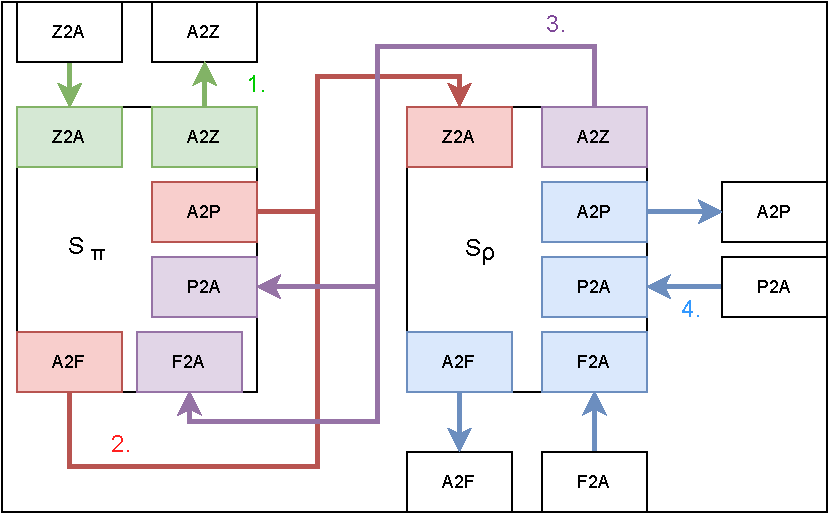
\includegraphics[scale=0.62]{figures/simcomp.pdf}
\caption{The composed simulators for $\F_1 \xrightarrow{\rho \circ \pi} \F_3$. The real world consists of $(\rho \circ \pi, \F_1)$. Inputs from \Z are for $\F_1$ and dummy parties interacting with $\F_1$, which \SIM{\pi} is equipped to handle. Outputs from \SIM{\pi} are for $\F_2$ and dummy parties of $\F_2$ which \SIM{\rho} is equipped to handle. FInally, outputs from \SIM{\rho} are for $\F_3$ and dummy parties of $\F_3$, which is just the ideal world in Theorem~\ref{thm:composition}.}
\label{fig:simcomp}
\end{figure}

%\begin{lstlisting}[basicstyle=\small\BeraMonottFamily, mathescape, frame=single]
%m = recv $\$$p2a ;
%case m (
%  P2A(pid, msg) =>
%   	case msg (
%      Committed =>
%        h = sample r k ;
%        send $\$$z2a P2A2Z(pid, (h)) ;
%      Open(b) =>
%	    x = sample r k ;
%        send $\$$z2a P2A2Z(pid, SMsg(b, x)) ;
%\end{lstlisting}

%When the committer is corrupt, the simulator has to do more work. 
%The key point that makes commitment in the RO model realizable is that \Z acquires commitment to give to the corrupt committer from \Fro through \A. 
%In th ideal world, the simulator recrods all the (key,value) pairs generated by its simulation of \Fro and therefore can always determine the bit \Z is committed to.
%When \Z queries \Sim with \inline{Z2A2F(SHash(b + x))} it stores the value and generates a hash value for it and returns it to \Z. 
%When instructed to give input to the corrupt party the simulator, \Sim gives input \inline{A2P(1, Commit(b))} where $b$ is the bit whos hash was requested.
%
%There is a unique edge case where \Z give some random bit sequence to \S as the commitment which wasn't generated by the random oracle. 
%In this case \S chooses a bit at random annd passes \inline{A2P(1, Commit(b))} to the protocol wrapper where $b$ is randomly selected.
%When prompted to open the commitment, \S does nothing as the real world receiver would fail to confirm whether the commitment corresponds to the bit $b$.




%\subsection{Ideal World}
%We described the functionality \Fcom in detail in Section~\ref{sec:execuc} as well as the functionality wrapper construction around it.
%We now describe how we implement ideal world (dummy) parties.

%We first describe at a high-level, the conversion happening within the functionality wrapper for \Fcom with the \inline{commit} message sent by the sender.
%When the wrapper receives the \inline{commit} message, the functionality wrapper executes the following:
%\begin{lstlisting}[basicstyle=\small\BeraMonottFamily, frame=single, mathescape]
%$\tg{(* l1 : list[pid \textasciicircum sender] *)}$
%case $\$$p2f (
%  yes => 
%    pid = recv $\$$p2f ; msg = recv $\$$p2f ;
%    case msg (
%      Commit(b) => 

%        $\$$ch_ = get_channel_by_pid pid $\$$l1 $\$$l2 ... ;
%        $\$$ch_.commit ;
%        send $\$$ch_ b ;
%        $\$$l2' <- append $\$$ch_ $\$$l2 ;
%\end{lstlisting}
%The wrapper also spawns a process to read from each of \Fcom's outgoing channels, case analyze on their value and send out the corresponding functional message to the protocol wrapper.

%The \msf{execUC} function in Figure~\ref{lst:execuc} accepts some number of type parameter which it spawns the main channels of the protocol with. 
%Most important out of these channels is the types governing communication between \Z and \A and between \Z and the protocol wrapper.
%If the types for these channel in both worlds aren't the same, even the import token expected, then it is trivial for an environment to distinguish the two worlds.
%It suffices to specify the import type parameters (\inline{p2f}, \inline{f2p}, \inline{z2p}, etc.) to \inline{execUC}.
%\paragraph{The Ideal World Execution}
%We summarize the message types in use by describing the type parameters to the ideal world execution.
%For the ideal, \inline{execUC} is invoked as follows (refer to the \inline{execUC} definition in Figure~\ref{lst:execuc} for what each of the parameters refers to):
%\begin{lstlisting}[basicstyle=\small\BeraMonottFamily, frame=single, mathescape]
%$\Type$ z2amsg[a][b] = Z2A2P of pid ^ a 
%                     | Z2A2F of b ;
%$\tg{(* ideal world *)}$
%execUC[K1,K2][comf2p][comp2f][comp2f][comf2p]
%  [comf2p][comp2f][comf2a][coma2f][rof2a][roa2f]
%  [rof2p][rop2f]
%\end{lstlisting}
%%$\tg{(* real world *)}$
%%execUC[K1,K2][comf2p][comp2f][rop2f][rof2p]
%%  [rof2p][rop2f][comf2a][coma2f][rof2a][roa2f]
%%  [rof2p][rop2f]
%Notice that the message types over \inline{p2z} and over \inline{p2f} are the same, because the ideal world parties are dummy parties which simply forward the messages to \Fcom.
%The type parameters for the adversary in the ideal world, though, still take the form of the types of \Fro.
%This is because the inputs \Z gives to both worlds (the dummy adversary in the real world) is intended for \Fro when communicating with the functionality through the adverasary or through corrupt parties 
%
%The party inputs from \inline{a2p} in the ideal world are intended for \Fcom, not \Fro, so they are of the same type \inline{comp2f}.
%Similarly, output from corrupt parties to the adversary in the ideal world is the same as output from \Fcom, and, therefore the message type is the same as \inline{comf2p}.
%The messages type parameters are wrapped in channel-specific types as well.
%For example, the channel \inline{z2a} is typed as follows:
%\begin{lstlisting}[basicstyle=\small\BeraMonottFamily, frame=single, mathescape]
%type z2amsg[a][b] = Z2A2P of pid ^ a
%                      | Z2A2F of b ;
%#z_to_a: comm[z2amsg[a2p][a2f]]
%$\tg{(* a2p=rop2f, a2f=roa2f in execUC above*)}$
%\end{lstlisting}
%
%\paragraph{Ideal Protocol}
%The ideal world protocl is a dummy party which forwards all messages to the functionality. 
%The message content from \inline{z2p} and \inline{p2f} is the same in the ideal world, but it is wrapped in different parameteric typed when it is sent from the \inline{z} or \inline{p}.
%As shown below the messages themselves are the same (\inline{comp2f} but typed differently (\inline{z2pmsg} vs \inline{p2fmsg}):
%\begin{lstlisting}[basicstyle=\small\BeraMonottFamily, frame=single, mathescape]
%$\Type$ z2pmsg[a] = Z2P of pid ^ a ;
%$\Type$ p2fmsg[a] = P2F of pid ^ a ;
%#z_to_p: comm[z2pmsg[comp2f]] ;
%#p_to_f: comm[p2fmsg[comp2f]] ;
%\end{lstlisting}
%The protocol wrapper only needs to forward the message unaltered but using a different type construtor. 

%The ideal functionality \Fcom is the same one introduced in Figure~\ref{fig:fcom} in Section~\ref{sec:nomosuc}. 
%In FIgure~\ref{lst:fcom} we present the Nomos definition of the same functionality and provide the channel types in FIgure~\ref{fig:fcomtypes}.
%We elide some of the clutter of acquiring and releasing shared channels in the form of: \texttt{\$p2f $\leftarrow$ acquire \#p\_to\_f} for clarity. 
%Wherever a linear channel like \texttt{\$p2f} is used it is in fact an acquired shared channel \texttt{\#p\_to\_f}.
%
%The key difference to note between \Fcom and its Nomos version is that the functionality is split up into two processes rather than compressed into one.
%This design decision is required because of how Nomos cycles between processes in a round-robin fashion and the communicator design.
%Therefore, processes must recurse when there is no message to be read and move to the next processes after the first expected message is received--in this case the \msf{P2FCommit(b)} message.
%
%
%\begin{figure}
%\centering
%\msf{type} \msf{Ip2f} = \msf{P2FCommit} of \msf{Bit} | \msf{P2FOpen}
%
%\msf{type} \msf{If2p} = \msf{F2PCommit} | \msf{F2POpen} of \msf{Bit}
%
%\msf{type} \msf{Ip2f} = \msf{SCommit} of Bit | \msf{SOpen}
%
%\msf{type} \msf{If2p} = \msf{RCommit} | \msf{ROpen} of Bit
%
%\msf{type} \msf{Rp2f} = \msf{SHash} of \msf{Int} | \msf{Send} of \msf{pid} \textasciicircum \msf{pid} \textasciicircum \msf{Int}
%
%\msf{type} \msf{Rf2p} = \msf{Pre} of \msf{Int} | \msf{RHash} of \msf{Int} | \msf{MSG} of \msf{pid} \textasciicircum \msf{pid} \textasciicircum \msf{Int}
%
%\caption{Types for the channels in the ideal world for \Fcom. Notice that Ip2f and If2p is the type of the channels \msf{z2p} and \msf{p2z} as they much match for both worlds and the ideal world parties simply forward messages to the functionality. The \msf{p2f} and \msf{f2p} channels are specific to the real and ideal world as the functionalities are not the same. Hence the real-world \msf{p2f} is typed with \msf{Rp2f} for the random oracle and the ideal world \msf{p2f} is typed with \msf{Ip2f} for \Fcom.}
%\label{fig:fcomtypes}
%\end{figure}
%
%\begin{figure*}
%\begin{lstlisting}[basicstyle=\small\BeraMonottFamily]
%proc F_code:
%  (s: sid), (k: Int), (rng: [Bit]), (clist: list[Int]),
%  (#p_to_f: comm[pid ^ Ip2f]{Ip2fn}), (#f_to_p: comm[pid ^ If2p]{If2pn}),
%  (#a_to_f: comm[Ia2f]{Ia2fn}), (#f_to_a: comm[If2a]{If2an})  |- ($ch: FtOE) =
%{
%  case $p2f (
%    yes =>	
%      pid, msg = recv $p2f ;
%      get $pwf {Ip2fn} ;
%      case msg (
%        P2FCommit(b) =>	
%          if pid == 1
%          then
%            send F2PCommit $f2p ;
%            pay {If2pn} $f2p ;
%            $ch <- F_com_open s k rng clist #p_to_f #f_to_p b ;
%          end
%      )
%   | no =>  
%       $ch <- F_code s k rng clist #p_to_f #f_to_p ;
%  )
%}
%
%proc F_code_open:
%{
%  case $p2f (
%    yes =>	
%      pid, msg = recv $p2f ;
%      get $p2f {0} ;
%      case msg (
%        P2FOpen =>	
%          if pid == 1
%          then
%            send F2POpen(b) $f2p ;
%            pay {0} $f2p ;
%            $ch <- 1 ;
%          end
%      )
%   | no =>
%       $ch <- F_code_open s k rng clist #p_to_f #f_to_p b ;
%  )
%}
%\end{lstlisting}
%\end{figure*}
%
%The real world protocol for commitment follows a simple communication patter:
%\begin{enumerate}
%\item On input bit $(\msf{P2FCommit}\ b)$ from the environment, the committer queries the random oracle with the message $(\msf{SHash}\ b | r)$ where $r \xleftarrow{\$} \{0,1\}^k$.
%The returned ``hash value'' is sent to the receiver as the commitment.
%\item On input \msf{P2FOpen} from \Z, the committer sends $(\msf{Send}\ p_L\ b\ r)$ to the receiver.
%\item The receiver checks that the commitment is correct be querying \Fro in the same way and asserting that the has returned $(\msf{RHash}\ h)$ is the same as the one sent by $p_C$.
%\item \todo{the type of Rf2p is kind of wrong so need to correct it}
%\end{enumerate}
%
%We provide only a simulator for the dummy adversary as that guarantees a simulator for all adversaries required our emulation definition.
%The simulator for commitment is relatively simple so we only provide a high-level description here and leave the full simulator code to the appendix.
%The simulator internally simulats the random oracle by maintaining a table of key-value pairs that it can control entirely.
%If the committer is corrupt:
%\begin{enumerate}
%\item The simulator can not determine the bit \Z wants to commit to so selects a random bit when activatd by the environment and gives it as input to the corrupted committer.
%\item When it's asked to open the commitment it simply forwards the request to the corrupt committer and stops.
%\end{enumerate}
%If the receiver is corrupt:
%\begin{enumerate}
%\item When activated by the receiver with (\msf{F2PCommit}), the simulator generates some random string $h$ to represent the commitment, stores it, and sends ($\msf{P2A}\ \msf{MSG}(p_C, p_R, h)$) to \Z.
%\item When it receives ($\msf{F2POpen}\ b$) from the receiver, it returns $(\msf{P2A}\ \msf{MSG}(p_C, p_R, b, r)$ to \Z where $r$ is a randomly generated sequence keeping the pair $(b | r, h)$ as the corresponding entry in the table.
%\item When activated by \Z to check the commitment, \Sim simply returns the commitment hash or creates a new one.
%\end{enumerate}
%
%\paragraph{Simulator Well-Matched}
%It is immediately obvious that the constructed simulator is well-typed if the dummy adversary is well-typed with the given type parameters.
%The simulator receives 1 import token per activation from \Z which suffices to simulated \Fro internally. 
%Subsequently, \Sim keeps all of the import it receives, and, therefore when one of the partiesis corrupt a simple bounding polynomial can be given as:
%\[
%	T_{\Dummysim}(n) = T_{\Fro}(n) + O(1)
%\]
%where $T_{\Fro}$ is a satisfying polynomial for \Fro. The additional constant factor simply accounts for sending messages to the corrupt parties.
%Therefore,
%\begin{gather}
%	\forall \Z, \langle \Z \leftrightarrow \DA \rangle \Rightarrow \langle \Z \leftrightarrow \Dummysim \rangle
%\end{gather}
%
%
%\begin{figure*}
%\begin{lstlisting}[basicstyle=\BeraMonottFamily]
%(* Z2P interface *)
%type Ip2f = P2FCommit of Bit | P2FOpen ;
%type If2p = F2PCommit | F2POpen of Bit ;
%
%(* Ideal World *)
%type Ip2f = SCommit of Bit | SOpen ;
%type If2p = RCommit | ROpen of Bit ;
%
%type Ia2f = 0 ;
%type If2a = 0 ;
%
%type Ia2p = Ip2f ;	(* crupt input is same as z2p *)
%type Ip2a = If2p ;
%
%(* Real World *)
%type Rp2f = SHash of Int | Send of pid ^ pid ^ Int ;
%type Rf2p = Pre of Int | RHash of Int | MSG of pid ^ pid ^ Int ;
%
%type Ra2f = A2Hash of Int ;
%type Rf2a = Hash2A of Int ;
%
%type Ra2p = Rp2f ;
%type Rp2a = Rf2p ;
%
%(* the import here is given as those for the dummy adversary in the real world *)
%p2zn <- 0 ; z2pn <- 1 ;
%a2zn <- 0 ; z2an <- 1 ; 
%
%Rf2pn <- 0 ; Rp2fn <- 1 ;
%Rp2an <- 0 ; Ra2pn <- 1 ;
%Rf2an <- 0 ; Ra2fn <- 1 ;
%
%If2pn <- 0 ; Ip2fn <- 0 ;
%Ip2an <- 0 ; Ia2pn <- 0 ;
%I
%
%(* channels *)
%#z_to_p <- comm[pid ^ Ip2f]
%#p_to_z <- comm[pid ^ If2p]
%#z_to_a <- comm[ z2d[Ra2p][Ra2f] ] ;
%#z_to_z <- comm[ d2z[Rp2a][Rf2a] ] ;
%
%
%(* Real World exec PI *)
%execUC[Ip2f][If2p][Rp2f][Rf2p][Rp2a][Ra2p][Rf2a][Ra2f][a2z][z2a]
%	  {p2zn}{z2pn}{f2pn}{p2fn}{p2an}{a2pn}{f2an}{a2fn}{a2zn}{z2an}
%
%(* Ideal world exec PHI *)
%execUC[If2p][Ip2f][Ip2f][If2p][Ip2a][Ia2p][If2a][Ia2f][a2z][z2a]
%	  {p2zn}{z2pn}
%
%
%
%
%
%
%\end{lstlisting}
%\end{figure*}


The type system in NomosUC helps to identify when the amount of potential that a functionality requires isn't satisfied by the bounding polynomia given.
We illustrate this point using the $\F_{\msf{map}}$. 
The functionality maintains a list that parties can append to the end of or read from.




\section{Related Works} \label{sec:related}
There is a large volume of work that introduces tools for modeling UC protocols and reasoning about UC security.
Some even mechanize UC proof-generation~\cite{certicrypt, easycrypt, cryptoverif, cryptol, fstar}.
However, unlike our work, many of them only do so in the standalone setting without any composition guarantees.
They also do not completely capture a robust polynomial-time notion or realize generalized composition. 

Canetti et al.~\cite{easyuc} and Barbosa et al.~\cite{barbosa} both build off EasyCrypt's game-based security definitions to reach UC-like simulation-based definitions.
They both mechanize security proof generation and allow more complicated reasoning for indistinguishability given a formal term capping the environments capabilities. Out work, like ILC defines indistinguishability in terms of a security parameter $k$, but without any program logic for security. 
Barbosa introduces a limited polynomial time notion for its definitions, whereas EasyUC~\cite{easyuc} does not encode any runtime guarantees in its programs. 
For example, it cannot detect indefinite message passing between \A and \F. Neither, however, capture full UC composition.
Barbosa realizes simplified UC~\cite{suc}, and, like EasyUC, does not capture dynamic party creation or the multisession operator.
In contrast, NomosUC derives a polynomial-time bound on ITMs statically with a proof that the computed bounds are correct.

%EasyUC~\cite{easyuc} introduces a toolset built on top of the existing EasyCrypt~\cite{easycrypt} toolset to model UC protocols and generate proofs of security.
%It moves past the game-based security limitation of EasyCrypt and achieves the broader simulation-based definitions of UC, but does not encode any runtime guarantees.
%%EasyUC mechanizes UC's notion of simulation-based security and formally verifies UC realization--something Nomos doesn't attempt to do.
%%The major limitation of EasyUC is that it does not encode any guarantees on the runtime of any process.
%For example it can not detect a functionality and the adversary can exchange messages \emph{indefinitely} in their key exchange example. It also can not capture full UC composition because it is limited to a statically determined number of parties in any execution.
%%NomosUC, on the other hand, proposes the full UC composition theorem, a robust polynomial time notion that relies on the import mechanism introduced in UC, and a full expressive language that can support arbitrary UC executions.
%
%Barbosa et al.~\cite{barbosa} builds off EasyCrypt as well, but introduce a polynomial time notion to their handling of UC. 
%However, it is limited by the procedure call commnication method of EasyCrypt, limiting expressiveness, and only realizes the simplidied SUC~\cite{suc} without dynamic party creation.
%%They're able to relate the guarantees provided by EasyCrypt to the execution time of an adversary that can break the security of the protocol. 
%%Barbarosa also must contend with the procedure call communication of EasyCrypt limiting the expressiveness of the framework. 
%%Furthermore it suffers similar drawbacks to EasyUC, and all works mentioned in this section, in that does not fully capture dynamic party creation in UC, and they realize only a simplified version of UC~\cite{suc}.

ILC proposed by Liao et al.~\cite{ilc} is another work closely related to ours which introduced the idea of using a write token
to resolve read and write non-determinism.
But it suffers some of the same drawbacks as EasyUC and the work of Barbosa et al.~\cite{barbosa},
because it does not support full composition and is also limited to a static number of parties in its UC definition.
It improves on EasyUC and provides a polynomial time notion, but ends up requiring simulation in both directions to prove emulation. 
This means that even simple protocols like a ping-response server cannot be judged secure.

The work on IPDL~\cite{ipdl} by Morrisett et al. also aims to mechanize proofs of security and improves upon EasyUC by providing a better notion of emulation,
more akin to the UC framework, and symbolically tracks the run time of straight-line programs (and those with statically upper-bounded loops).
IPDL further implements a unique communication mechanism that imposes a static dependency between channels ``firing''.
%It symbolically tracks the run time of programs but can only do so for straight-line programs or those with statically upper-bounded loops.
However, it precludes expressing constructs like the multisession operator, presented later in this work. 
%The operator allows creation of an arbitrary number of subsessions of a functionality and is critical to realizing the full UC composition theorem.

We summarize the imporant features of the most closely related work to NomosUC in Figure~\ref{fig:relatedworks}.
%The columns are broken up according to the features mentioned in the above discussion.
The first row discusses whether the environment can create an arbitrary number of parties at runtime. %There is no partial-support in this category, either it is supported or it isn't.
The second row broadly covers whether there is any restricted or full support for runtime or polynomial-time analysis or dynamic tracking. %restricted poly time (partiais performed by the project
%Notice that there is partial support where ILC provides a restricted notion of polynomial time.
The third row determines whether full UC-style composition is supported, i.e. replacement of an arbitrary number of functionalities with realizing protocols (the existence of a multisession operator is essential). 
The last row highlights a design choice in communication through channels or through programming-style procedure calls.
The distinction plays an important role in how communication is captured in each work, and whether arbitrary communication patterns from UC are not fully supported.

% Colums: blank | parties at runtime | notion of UC | polynomial time | generalized composition operator | channels | procedural 
\begin{figure}[H]
\centering 
\begin{table}[H]
	\vspace{-2em}
	%\scalebox{0.7}{\begin{tabular}{l | c  c  c  c  c}
	%& \rot{Dynamic \# Parties} & \rot{Polytime Notion} & \rot{General Composition} & \rot{\parbox{3cm}{Channels/Procedures}} \\
	%\hline
	%IPDL~\cite{ipdl} & \emptycirc[0.75ex] & \fullcirc[0.75ex] & \fullcirc[0.75ex] & Channels \\
	%%\hline
	%EasyUC~\cite{easyuc} & \emptycirc[0.75ex] & \emptycirc[0.75ex] & \emptycirc[0.75ex] & Procedure Calls \\
	%%\hline
	%Barbosa et al.~\cite{barbarosa} & \emptycirc[0.75ex] & \fullcirc[0.75ex] & \fullcirc[0.75ex] & Procedure  Calls \\
	%%\hline
	%ILC~\cite{ilc} & \emptycirc[0.75ex] & \halfcircleft[0.75ex] & \emptycirc[0.75ex]  & Channels    \\
	%%\hline
	%NomosUC (this work) & \fullcirc[0.75ex]  & \fullcirc[0.75ex]  & \fullcirc[0.75ex]  & Channels  \\
	%%\hline
	%\end{tabular}}
	\scalebox{0.7}{\begin{tabular}{l | c  c  c  c  c}
	& IPDL & EasyUC & Barbosa et al. & ILC & \textbf{NomosUC}\\
	\hline
	Dynamic \# of Parties & \emptycirc[0.75ex] & \emptycirc[0.75ex] & \emptycirc[0.75ex] & \emptycirc[0.75ex] & \fullcirc[0.75ex] \\
	%\hline
	Polytime Notion & \fullcirc[0.75ex] & \emptycirc[0.75ex] & \fullcirc[0.75ex] & \halfcircleft[0.75ex] & \fullcirc[0.75ex] \\
	%\hline
	General Composition & \fullcirc[0.75ex] & \emptycirc[0.75ex] & \fullcirc[0.75ex] & \emptycirc[0.75ex] & \fullcirc[0.75ex] \\
	Security Proofs & \fullcirc[0.75ex] & \fullcirc[0.75ex] & \fullcirc[0.75ex] & \emptycirc[0.75ex] & \emptycirc[0.75ex] \\
	%\hline
	Channels/Procedures & Channels & Procedure Calls & Procedure Calls  & Channels & Channels 
	%\hline
	\end{tabular}}
\end{table}
\vspace{-1em}
\caption{Aspects covered by related works.
Empty circle \emptycirc[0.5ex] indicates no support, half circle \halfcircleft[0.5ex] indicates partial support,
and full circle \fullcirc[0.5ex] indicates full support.}
\vspace{-1em}
\label{fig:relatedworks}
\end{figure}

\paragraph*{\textbf{Session Types}}
On a different thread, the core calculus of NomosUC is inspired from resource-aware session types~\cite{das2018work} which combines
session types~\cite{HondaCONCUR1993, HondaESOP1998, HondaPOPL2008,caires2010session, ToninhoESOP2013, PfenningFOSSACS2015,
WadlerICFP2012} and automatic amortized resource analysis~\cite{Hofmann03AARA,HoffmannW15}.
We build off binary session types in this work, however other formuations such as multi-party session types exist that allow describing a protocol between many processes rather than bi-directional~\cite{Capecchi10CONCUR}.
Though appearing as a better fit, multiparty session types are not well-suited for dynamic creation of parties since they require statically specifying a global communication protocol between all processes.
This would not allow for the possibility of spawning a dynamic (or even static) number of processes in the middle of a communication, which is central to UC.
Moreover, binary session types also provide support for cost analysis that is fundamental to the import mechanism, a core contribution of our work.

%Session types were introduced by Honda et al.~\cite{HondaCONCUR1993} to describe and enforce bi-directional communication protocols
%in message-passing systems.
%Resource-aware session types~\cite{das2018work} add potential annotations to session types for execution cost analysis
%of distributed protocols.
%Another formulation of session types that aren't binary~\cite{Derakhshan21LICS} are multiparty-session types~\cite{Capecchi10CONCUR} that
%More related to security, recent work has integrated session types with information flow type systems, both
%in the binary~\cite{Derakhshan21LICS} and multiparty~\cite{Capecchi10CONCUR} setting.
%The former uses logical relations to define non-interference while the latter
%guarantees a form of access control and secure information flow.

%There is large body of similar work that introduces process calculi, some extensions of $\pi$-calculus, like ILC.
%Mateus et al.~\cite{mateus} for example introduces process calulus for simpler, sequential composition but is constraints to a schedular-based construction where probabilistic state transitions follow unifor distribution at every step.
%SymbolicUC~\cite{symbolicuc} \todo{finish oter symbolic logic and state their weaknesses and that ther are subsumed by ILC}.
%
%NomosUC adds to the body of prior work by using resource-aware session types~\cite{das} to describe protocols, functionalities, and their behavior. 
%Session types express the steps and communication in a protocol at the type level, and offer greater tooling for creating large protocols with smaller, modular pieces. 
%Resource-aware session types add a mechanism called potential, that we use to implment the import mechanism described in the UC framework.
%Import provides a more precise notion of polynomial time in UC (refer to the UC framework~\cite{UC}), and, to the best of our knowledge, this is the first such work to implement and create tooling around it. \todo{surely there is better wording than ``create tooling around it'' to get across the point I'm trying to make}.

%One of the most relevant works to our own is EasyUC~\cite{easyuc}. 
%EasyUC uses the existing EasyCrypy~\cite{easycrypt} toolset to model UC protocols and mechanize proof generation. 
%It departs from EasyCrypt's limtations to game-based security definitions (lacking simulation-based composition).
%However, it still lacks a notion of polynomial time. The authors, themselves, mentions that it can't detect deviant behavior like the adversary and functionality passing messages between each other indefinitely. 
%Our use of the import mechainsm and session types let us reason about polynomial time in the sytem of ITMs encompassed by \msf{execUC} but also locally for \textit{open} terms. 
%Furthermore, import in NomosUC lets us have guarantees of termination as well by the polyomial import constraints added to UC by Canetti et al.
%
%Liao et al. introduce executable UC through a new process calculus called ILC~\ref{ilc}.
%This work adds some notion of polynomial time although it proves to be too restrictive. 
%It results from the fact that poly-time can only be reasoned about for \textit{closed} terms like a full UC execution.
%In order to reason about polynomial time for a particular protocol $\pi$ we must reason over all possible other terms that connect to $\pi$ and require that it is polynomial in all such cases.
%A simple ping-response server can not be proven to by poly-time in this definition for a deviant other ITM that connects to $\pi$. 
%In Nomos, however, as mentioned above, open terms are limited to polytime regardless of the connected other terms because of the import mechanism and the NomosUC type system that guarantees termination. 
%
%Other works that rely in symbolic modelling of cryptography, for example, SymbolicUC~\cite{symbolicuc}, are subsumed by the above ILC work and similarly lack any polynomial time notion. 
%\todo{Say something about $\pi$-calculus with probabilistic polynomial time extensions}.
%
%To the best of our knowledge, this is the first work to deal with the new import notion of polynomial time introduced to the UC framework in 2018.
%A few other works refer to the import mechanism, but it is restricted to simply defining the import a protocol is given.

%\begin{figure*}
%\begin{center}
%\begin{tabularx}{\textwidth}{|p{0.2\textwidth}|p{0.2\textwidth}|p{0.2\textwidth}|p{0.2\textwidth}|}
%\hline \\
%        & Polynomial-time termination                                  & simulator type mismatch                             & emulation fully proven \\ 
%\hline \\
%NomosUC & Guaranteed termination, local polynomial time for open terms & PPT Simulator under import constraints of adversary &  \\
%\hline \\
%IPDL    & Statically typed loops and straightline programs only        & 													 & proof generation and full emulation \\
%\hline \\
%EasyUC  & No polynomial time guarantee or guaranteed termination       & 													 & machine checked \\ 
%\end{tabularx}
%\end{center}
%\end{figure*}

%easyUC:
%* can not dynamially create new instances of parties/functionalities must statically determine the number of functionalities/parties spawned
%* 
%
%
%The work of Liao et al.~\ref{ilc} is the closest to our own
%It proposes a new process calculus called ILC and a concrete implementation of the UC framework.
%The type system it introduces ensures that correctly types programs can be represented as ITMs.
%However, one drawback of the ILC work is that its polynomial time representation 
%
%
%The EasyUC approach uses the existing EasyCrypt toolset to implement model UC protocols and mechanize the generate of UC-security proofs and proofs of secure composition.
%This work aim considerably higher than our work in actually attempting to generate proofs for their protocols. 
%However, this work falls short in being able to capture any notion of resource bound computation whereas we are able to make guarnatees about polynomial bounds on our system of ITMs and even guarantee termination of programs through our realization of the import mechanism.
%The EasyUC work accepts that not even infinite loops of communication can be caught and, therefore, termination of protocols can't be guarnateed either whereas the import mechanism in Nomos ensures that such infinite loops can not stall protocol progress.

%Another work similar to our own is the Symbolic UC by B\"{o}hl and Unruh.
%This works uses an applied $\pi$-calculus to symbolically model UC protocols and analyze them.
%Similar to the EasyUC work, the goals of this work are somewhat orthogonal to the our own goals.
%However, Symbolic UC does attempt to create an implementatio of UC using the $\pi$-calculus however neglects to address any issues of polynomial runtime.
%
%Perhaps the closes work to our own is that of Liao et al.~\cite{ilc} that builds an executable version of the UC framework by introducing a new process calculus called ILC.
%ILC introduces a type system that guarantees that ILC programs (i.e. functionalities, protocols, etc) can be expressed as ITMs as in the UC framework.
%However, one drawback of ILC is that it's notion of polynomial time ends up being too restrictive.
%In ILC only closed terms without any unbonded variables, i.e. and entire UC exection of a system of ITMs, can be shown to be polynomial in their definition of polynomial time.
%Proving polynomial time for open terms, such as a protocol $\pi$, requires reasoning over all possible contexts in which the protocol could exist however such a definition of polynomial time becomes too restrictive where even a simple ping-responde server protocol wouldn't be considered polynomial time.


\section{Conclusions and Future Work}
This area of research presents several next steps and possibility for futurework building on NomosUC.

On of the immediate next steps is to overcome the existing Nomos provider-client constraints. 
Currently, we introduce a several channels and a couple of commuicators to generalize communication between two processes. 
This is due in large part to linear channels being unique to a specific provider and client.
We would like to do away withthis requirement in subsequent works and grealy simplify our construction.

We also point out that we build NomosUC on top of the type system defined by Nomos, however, we do not yet implement a type checker for NomosUC. We rely on the typing rules and theorems to validate our approach and manually typed checked the functionalities, protocols, and simulator code we implemented.
A next step in this direction is attempting to implement the type checker for NomosUC or evaluating the feasibility of doing so.

A few works related to our own, described in Section~\ref{sec:related}, attempt to automate proof generation for composable security. Our work provides tooling to specify and analyze UC definitions, however, a goal of future work is to introduce fuzz testing of protocols, functionalities, and emulation in NomosUC.



\bibliographystyle{IEEEtran}
\bibliography{nomosuc}

\newpage

%input{figures/asyncwrapper}

%\appendix
\appendices

\section{Simulators} \label{sec:commitment}
In this section we work throgh the entire commitment example that has seen used throughout this paper, and we show composition by realizing a coin flipping ideal functionality \Fflip and a protocol realizing it in the \Fcom-hybrid world.
We present the random oracle functionalitt \Fro, the real world protocol \prot{com}, and a simulator for the dummy adversary.
Along the way we address the apparent import mismatch between \Fcom and \Fro, and we discuss how emulation and composition work around it.
Finally, we give \Fflip, and a realizing protocol and sketch the composed simulator for $\Fro \xrightarrow{\prot{flip} \circ \prot{com}} \Fflip$.

%\subsection{Static Corruptions}
%We deal in the static corruptions model of UC in this work. 
%This means that the environment decides the set of corrupt parties before the UC execution begins, and the adversary has no ability to corrupt any new parties mid-execution.
%The way NomosUC handles corrupt parties, and their inputs, is also how it handles ideal world (dummy parties).
%
%The dummy protocol does nothing but forward messages on its \inline{z2p} channel to its offered channel, and vice versa. 
%%Its code has the same type definition as any other protocol party but the code is trivial:
%%\begin{lstlisting}[basicstyle=\small\BeraMonottFamily, mathescape]
%%$\$$ch <- $\$$d ;
%%\end{lstlisting}
%%where \inline{$\$$d} is the channel it offers.
%%For honest and corrupt dummy parties in the ideal world, their incoming type from \Z or \A is the same and matches the type of the underlying \F.
%%It follows, then, that in the real world the type of \A's channel with the party is the same as that of \Fro.

\subsection{The Random Oracle}
The random oracle functionality captures an idealized hash function. It samples random strings of length $k$ as ``hash values`` and stores them in a table for deterministic hashes.
It allows both protocol parties and the adversary to request hashes from it.
We augment \Fro with a single communication channel allowing it parties to send messages to each other. One caveat from traditional communication
is that the protocol parties must poll \Fro for new messages. The augmented functionality is called \Fropp from now on.

The random oracle is differet from \Fcom in that it has one channel fo all parties to use. This is due to the fact that its function is the same for all parties.
Recall the session type and its struture disusse in Section~\ref{sec:execuc}. The augmented session type is given below:
%The design of the random oracle is different from \Fcom in that it has only one channel for all parties to communicate over.
%We discussed the unique structure of the session type for \Fro in Section~\ref{sec:execuc}: its type before and after interaction with a party is the same.
%This enables a dynamic set of parties to communicate with it by moving the \inline{pid} of the message sender/receiver into the type.
%Our augmented functionality's type retains this feature, as described by its session type:
%\begin{mathpar}
\begin{center}
\parbox{0cm}{
\begin{tabbing}
$\m{party}[a] = \textcolor{red}{\getpot^2} \ichoice{$\=$\mb{hash} : \m{pid} \arrow \m{int} \tensor \m{hashing}[a],$\\
\>$\mb{send} : \m{pid} \arrow \m{pid} \arrow \m{a} \tensor \m{party}[a],$ \\
\>$\mb{recv}: \m{pid} \tensor \m{newmsg[a]}}$ \\
$\m{hashing}[a] = \echoice{\mb{shash} : \m{pid} \arrow \m{int} \tensor \textcolor{red}{\paypot^1} \m{party}[a]}$ \\
$\m{newmsg}[a] = \echoice{ \mb{yes}: \m{pid} \arrow \m{pid} \arrow \m{a} \tensor \textcolor{red}{\paypot^1} \m{party}[a], \mb{no}: \m{pid} \tensor \m{party[a]}}$
%\end{mathpar}
\end{tabbing}}
\end{center}
Similarly, the functional types are given by:
%One side effect of the session types is that we modify the standard UC channel to require receivers to ask for new messages sent to them.
%We cannot directly deliver messages to their receivers, because the committer's and receiver's \inline{p2f} channel would end up with different types and back to \inline{party[a]}.
%The corresponding functional message type between the protocol wrapper and functionality is also updated with inputs for the channel:
\begin{lstlisting}[basicstyle=\footnotesize\BeraMonottFamily, mathescape]
$\Type$ rop2f[a] = QHash of $\tgr{Int}$ | Send of pid ^ a 
               | Recv ;
$\Type$ rof2p[a] = RHash of $\tgr{Int}$ | Yes of pid ^ a 
               | No ;
\end{lstlisting}

\subsection{Commitment Protocol}
The real world commitment protocol is constructed in the random oracle model in the way of ~\cite{hofheinz}.
Its incoming channel from \Z is typed identically to \Fcom to ensure that emulation and composition hold.

We include in Figure~\ref{lst:committed} the most important part of the protocol: how the sender computes the commitment for its input bit. The receivers check of the commitment follows the same pattern for querying hashes. 
The sender accepts a bit from its \inline{z2p} channel and generates a nonce to blind the bit through a \inline{sample} of randomness~\footnote{Blinding is necessary otherwise \A knows the pre-image and can query \Fro for its hash value.}.
It creates the commitment by sending \Fropp the blinded bit and receiving a hash value from \inline{p2f}.
Finally it sends the hash to the receiver (which has pid=2).

Conversely, the receiver must request the commitment \inline{h} message from \Fropp, notify \Z of the commitment, and, as shown in Figure~\ref{lst:receiver}, when it receives the bit and the nonce it checks that its hash with the commitment.
%$\tb{case}$ $\$$z2p (
%  commit => 
\begin{figure}
\begin{lstlisting}[basicstyle=\footnotesize\BeraMonottFamily, frame=single, mathescape]
b = $\tm{recv}$ $\$$z2p ;
bits = sample k rng ;
$\$$p2f.hash ;
$\tm{send}$ $\$$p2f pid ;
$\tm{send}$ $\$$p2f b + bits ;
$\tb{case}$ $\$$p2f (
  shash => 
    h = $\tm{recv}$ $\$$p2f ;
    $\$$p2f.send ;
    $\tm{send}$ $\$$p2f pid 2 hash;
\end{lstlisting}
\caption{The code for the committer in $\prot{com}$ when it receives a \msf{commit} message from \Z. It obtains a hash of the message from \Fropp over \msf{p2f} and sends it to the receiver (pid=2) through the same functionality.}
\label{lst:committer}
\end{figure}
%$\$$p2f.recvmsg ;
%$\tb{case}$ $\$$p2f (
%  Yes(p, h)
%  $\tm{recv}$ $\$$p2f ;
%...
%$\tm{send}$ $\$$p2f (b+h);
%...
\begin{figure}
\begin{lstlisting}[basicstyle=\footnotesize\BeraMonottFamily, frame=single, mathescape]
sender = $\tm{recv}$ $\$$p2f ;
(b,h) = recv $\tm{recv}$ $\$$p2f ;
$\tg{(* query the hash of b+h *)}$
h = $\tm{recv}$ $\$$p2f ;
$\yo{if}$ h == hash
$\yo{then}$
  $\$$z2p.open
\end{lstlisting}
\caption{The code for the receiver checks for a new message and receives the bit and nonce from the committer. If the hash of the bit and nonce matches the commitment it received, it returns \msf{open} to \Z to confirm the commitment.}
\label{lst:receiver}
\end{figure}

%The protocol works as follows:
%\begin{enumerate}
%\item When the committer receives a \inline{Commit(b)} message from \Z, it samples some random bits $r$ and generates a hash $h$ by sending \inline{SHash(b + r)} to \Fro.
%\item It then sends the commitment to the receiver who notifies \Z with a \inline{committed} message.
%\item Finally, when \Z instructs the committer to \inline{Open} the commitment, it sends bit \inline{b} and randomness \inline{r} to the receiver. The receiver checks the commitment, with \inline{b} and \inline{r}, against \Fro and outputs \inline{Open(b)} to \Z if it checks out.
%\end{enumerate}

\subsection{Simulation}
Finally, we present a simulator \simcom, for the dummy adversary, for which the \Fcom is realized by \prot{com} in the \Fropp-hybrid world.
The simulator is straightforward and internally maintains a table like \Fro and responds to the environments queries for hashes. 
When the receiver is corrupt:
\begin{itemize}
\item \simcom responds with \inline{P2A2Z(2, no)} to all messages by \Z to get a message from the functionality
\item On \inline{Committed} by the ideal receiver, \simcom generates a random $r$ and sends \inline{P2A2Z(2, RHash(h))}.
\item In \inline{Open(b)} from the ideal receiver, \simcom generates a random nonce $x$ and stores \inline{b+x : h} in its \Fro table, and sends \inline{Yes(1, (b,x))} to \Z when asked for messages for the corrupt receiver.
\end{itemize}

The corrupt committer is not much different from the above case. In this case
the simulator stores the bit $b$, the none $x$ and the corresponding hash $h$ that \Z uses to create a commitment.
When the simulator receives the message to send the commitment to the receiver, it tells the ideal world committer to commit to $b$, and when it's told to open the commitment it opens it in the ideal world. 

It is immediately clear that this simulator satisfied $\Fro \xrightarrow{\prot{com}} \Fcom$ for the dummy adversary.

\subsection{Coin Flipping}
We present secure coin flipping here as another example and one that makes use of our composition operator. 
Additionally, this example makes use of a neat trick we use to get more guarantees out of the NomosUC type system.
Securely flipping a coin is a basic cryptographic primitive whose ideal functilnalitt \Fflip is captured by the session types in Figure~\ref{fig:fflip}.
It's a 2-party protocol where one party is the initator of the flip and the other is a receiver.
The desired property is that the coin flip is entirely unbiased by either of the two parties. The corresponding ideal functionality \Fflip samples a bit from from its random tape and returns it as the coin flip.
\begin{figure}
\centering
\begin{lstlisting}[basicstyle=\footnotesize\BeraMonottFamily, frame=single, mathescape]
$\Type$ flipper[K] = +{ init: K -> flipped } ;
$\Type$ fflipped = +{ getflip: &{ flip: Bit * 1 ,
                                  noflip: fflipped }} ;
$\Type$ receiver[K] = +{ getflip: &{ flip: K -> Bit -> 1 ,
                                     noflip: recever[K] }} ;
$\Type$ adv[K] = &{ flipped: K -> deliver } ;
$\Type$ deliver = &{ askflip: +{ yes: deliver,
                                 no: deliver }}
\end{lstlisting}
\end{figure}

\Fflip only sends messages to the receiver when asked for the outcome of the flip with a \inline{getflip}. 
We augment the session type, and the corresponding ideal functionality, with a polymorphic \inline{K} to strengthen the type and ensure that the receiver can not receive anything from \inline{getflip} until the flipped sends something of type \inline{K} to \Fflip.
We concretize \inline{K} with the unit type \inline{()} at the protocol level as we only care about ordering in the functionality. 
This gives the type more power and allows the resulting functionality and protocol code to be simpler. 

The code for \Fflip is quite simple and shown below:
\begin{lstlisting}[basicstyle=\footnotesize\BeraMonottFamily, frame=single, mathescape]
$\nproc$ F_coinflip[K] :
  (k: Int), (rng: [Bit]), (sid: session[1]),
  ($\$$F: flipper[K]), ($\$$R: receiver[K]),
  ($\$$A: adv[K]) |- ($\$$c: 1) =
{
  $\ncase$ $\$$F (
    init =>
      x = $\nrecv$ $\$$F ;
      b = sample 1 rng ;
      $\$$A.flipped ;
      $\nsend$ $\$$A x ;
	  $\tg{(* wait for getflips *)}$
      $\$$f <- getflip_f <- b $\$$F ;
      $\$$r <- getflip_r[K] <- b x $\$$R ;
  )
}
\end{lstlisting}
We elide the code for \inline{getflip} although it is straightforward. 
The adversary decides whether to deliver the output flip to a party asking for it.
Much like the real-world case where the corrupt committer never opens its commitment, the simulator here can ensure that only the flipper receives the flip.
As the session type indicates, the adversary responds with a \inline{yes} or \inline{no} to deliver the flip.

%Upon a \inline{getflip} request, the adversary is activated and asked whether to deliver the outcome as shown in Figure~\ref{fig:optional}. 
%\begin{figure}
%\centering
%\begin{lstlisting}[basicstyle=\small\BeraMonottFamily, frame=single, mathescape]
%$\ncase$ $\$$F (
%  getflip =>
%    $\$$A.askflip ;
%    $\ncase$ $\$$A (
%      yes =>
%        $\$$F.flip ; send $\$$F b ;
%      no =>
%        $\tg{(* loop and wait for getflip *)}$
%    )
%)
%\end{lstlisting}
%\caption{} \label{fig:optional}
%\end{figure}

The protocol for the coin flip uses \Fcom. 
The flipper commits to a bit $b$, the receiver sends the flipper a random bit $r$ in return, the flipper opens its commitment, and both parties compute the flip as $r \oplus b$.
The simulator for this protocol to realize \Fflip is straightforward:
\begin{itemize}
\item If the flipper is corrupt, the simulator tells the flipper to \inline{init} the flip when the environment sends it a \inline{Commit b} message. It gets the flip outcome $f$ from the flipper and simulates the receivers random bit $r = f \oplus b$ for the environment. It never delivers the flip outcome to the receiver unless the environment instructs it to open the flipper's commitment. By setting $r = f \oplus b$, when the environment receives $f$ it can check that $r \oplus b = f$.
\item If the receiver is corrupt, the simulator waits for \Fflip to inform it that the flip was initiated. It simulates the \inline{Commit} message from \Fcom to the receiver, for \Z. When it receives the random bit that \Z wants the receiver to send, it gets the flip outcome from the receiver, computes $b = r \oplus f$ and sends \inline{Open b} to \Z. Again, \Z can verify $b \oplus r$ similar to the above case.
nl
\end{itemize}

\subsection{Composition}
We describe a composition theorem in the previous section and a composition operator for protocols.
Here we demonstrate how to compose the simulatlors from the two experiments to create a simulator to prove Theorem~\ref{thm:compose}.
Two simulators being composed are: \SIM{com} for $\Fro \xrightarrow{\prot{com}} \Fcom$ and \SIM{flip} for $\Fcom \xrightarrow{\prot{flip}} \Fflip$. 
The code for the composed is very similar to the simulator for the Dummy Lemma described in Section~\ref{sec:dummy} and expanded on in Appendix~\ref{app:dummy}.
The exact connects are different but it follows identical virtualization and sandboxing.
Therefore, we elide any code snippets from this secion and, instead, present a high-level description of the simulator.

For the sake of generality, we refer to protocols $\pi$, $\rho$, and functionalities $\F_1$, $\F_2$, and $\F_3$, where $\rho$ is \prot{flip}, $\pi$ is \prot{com}, $\F_1$ is \Fro, $\F_2$ is \Fcom, and $\F_3$ is \Fflip.
The numbered steps in the description below correspond to the numbered arrows in Figure~\ref{fig:simcomp}.
\begin{enumerate}
\item Input from \Z: \inline{Z2A2P(p, msg)} for dummy parties of $\F_1$ and \inline{Z2A2F(msg)} for $\F_1$  are forwarded to \SIM{\pi}, and, Outputs from \SIM{\pi}: \inline{F2A2Z(msg)} and \inline{P2A2Z(p,msg)} are forwarded to \Z unaltered.
\item Inputs from \SIM{\pi}: \inline{A2F(msg)} for $\F_2$ and \inline{A2P(msg)} for dummy parties of $\F_2$ are forwarded to \SIM{\rho} as \inline{Z2A2F(msg)} \inline{Z2A2P(p,msg)}, respectively.
\item Outputs from \SIM{\rho}: \inline{P2A2Z(p,msg)} from simulated parties of $\rho$  and \inline{F2A2Z(msg)} from the simulated $\F_2$ are forwarded to \SIM{\pi} as \inline{P2A(p,m)} and \inline{F2A(m)}, respectively.
\item Inputs from \SIM{\rho}: \inline{A2F(msg)} for $\F_3$ and \inline{A2P(p,msg)} for dummy parties of $\F_3$ are forwarded unaltered, and, Outputs from $\F_3$ and its ideal parties: \inline{F2A(msg)} from $\F_3$ and \inline{P2A(p,msg)} from its ideal parties is forwarded to \SIM{\rho} unaltered.
\end{enumerate}

\begin{figure}
\centering
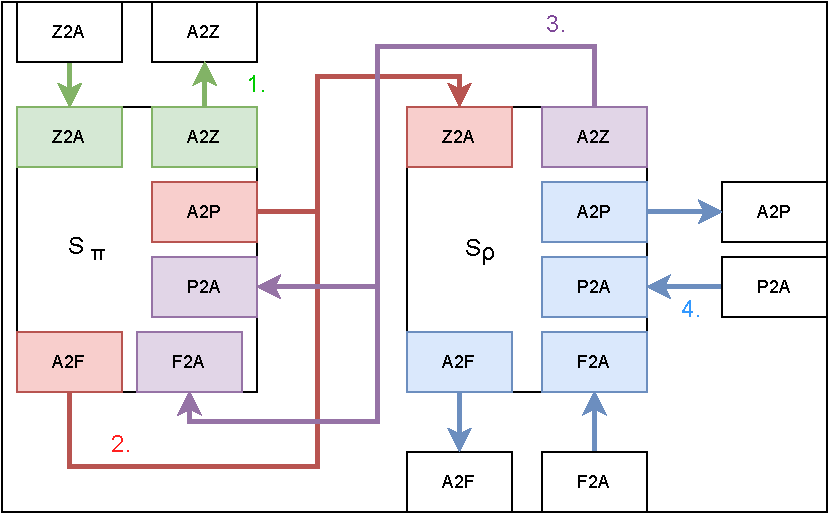
\includegraphics[scale=0.62]{figures/simcomp.pdf}
\caption{The composed simulators for $\F_1 \xrightarrow{\rho \circ \pi} \F_3$. The real world consists of $(\rho \circ \pi, \F_1)$. Inputs from \Z are for $\F_1$ and dummy parties interacting with $\F_1$, which \SIM{\pi} is equipped to handle. Outputs from \SIM{\pi} are for $\F_2$ and dummy parties of $\F_2$ which \SIM{\rho} is equipped to handle. FInally, outputs from \SIM{\rho} are for $\F_3$ and dummy parties of $\F_3$, which is just the ideal world in Theorem~\ref{thm:composition}.}
\label{fig:simcomp}
\end{figure}

%\begin{lstlisting}[basicstyle=\small\BeraMonottFamily, mathescape, frame=single]
%m = recv $\$$p2a ;
%case m (
%  P2A(pid, msg) =>
%   	case msg (
%      Committed =>
%        h = sample r k ;
%        send $\$$z2a P2A2Z(pid, (h)) ;
%      Open(b) =>
%	    x = sample r k ;
%        send $\$$z2a P2A2Z(pid, SMsg(b, x)) ;
%\end{lstlisting}

%When the committer is corrupt, the simulator has to do more work. 
%The key point that makes commitment in the RO model realizable is that \Z acquires commitment to give to the corrupt committer from \Fro through \A. 
%In th ideal world, the simulator recrods all the (key,value) pairs generated by its simulation of \Fro and therefore can always determine the bit \Z is committed to.
%When \Z queries \Sim with \inline{Z2A2F(SHash(b + x))} it stores the value and generates a hash value for it and returns it to \Z. 
%When instructed to give input to the corrupt party the simulator, \Sim gives input \inline{A2P(1, Commit(b))} where $b$ is the bit whos hash was requested.
%
%There is a unique edge case where \Z give some random bit sequence to \S as the commitment which wasn't generated by the random oracle. 
%In this case \S chooses a bit at random annd passes \inline{A2P(1, Commit(b))} to the protocol wrapper where $b$ is randomly selected.
%When prompted to open the commitment, \S does nothing as the real world receiver would fail to confirm whether the commitment corresponds to the bit $b$.




%\subsection{Ideal World}
%We described the functionality \Fcom in detail in Section~\ref{sec:execuc} as well as the functionality wrapper construction around it.
%We now describe how we implement ideal world (dummy) parties.

%We first describe at a high-level, the conversion happening within the functionality wrapper for \Fcom with the \inline{commit} message sent by the sender.
%When the wrapper receives the \inline{commit} message, the functionality wrapper executes the following:
%\begin{lstlisting}[basicstyle=\small\BeraMonottFamily, frame=single, mathescape]
%$\tg{(* l1 : list[pid \textasciicircum sender] *)}$
%case $\$$p2f (
%  yes => 
%    pid = recv $\$$p2f ; msg = recv $\$$p2f ;
%    case msg (
%      Commit(b) => 

%        $\$$ch_ = get_channel_by_pid pid $\$$l1 $\$$l2 ... ;
%        $\$$ch_.commit ;
%        send $\$$ch_ b ;
%        $\$$l2' <- append $\$$ch_ $\$$l2 ;
%\end{lstlisting}
%The wrapper also spawns a process to read from each of \Fcom's outgoing channels, case analyze on their value and send out the corresponding functional message to the protocol wrapper.

%The \msf{execUC} function in Figure~\ref{lst:execuc} accepts some number of type parameter which it spawns the main channels of the protocol with. 
%Most important out of these channels is the types governing communication between \Z and \A and between \Z and the protocol wrapper.
%If the types for these channel in both worlds aren't the same, even the import token expected, then it is trivial for an environment to distinguish the two worlds.
%It suffices to specify the import type parameters (\inline{p2f}, \inline{f2p}, \inline{z2p}, etc.) to \inline{execUC}.
%\paragraph{The Ideal World Execution}
%We summarize the message types in use by describing the type parameters to the ideal world execution.
%For the ideal, \inline{execUC} is invoked as follows (refer to the \inline{execUC} definition in Figure~\ref{lst:execuc} for what each of the parameters refers to):
%\begin{lstlisting}[basicstyle=\small\BeraMonottFamily, frame=single, mathescape]
%$\Type$ z2amsg[a][b] = Z2A2P of pid ^ a 
%                     | Z2A2F of b ;
%$\tg{(* ideal world *)}$
%execUC[K1,K2][comf2p][comp2f][comp2f][comf2p]
%  [comf2p][comp2f][comf2a][coma2f][rof2a][roa2f]
%  [rof2p][rop2f]
%\end{lstlisting}
%%$\tg{(* real world *)}$
%%execUC[K1,K2][comf2p][comp2f][rop2f][rof2p]
%%  [rof2p][rop2f][comf2a][coma2f][rof2a][roa2f]
%%  [rof2p][rop2f]
%Notice that the message types over \inline{p2z} and over \inline{p2f} are the same, because the ideal world parties are dummy parties which simply forward the messages to \Fcom.
%The type parameters for the adversary in the ideal world, though, still take the form of the types of \Fro.
%This is because the inputs \Z gives to both worlds (the dummy adversary in the real world) is intended for \Fro when communicating with the functionality through the adverasary or through corrupt parties 
%
%The party inputs from \inline{a2p} in the ideal world are intended for \Fcom, not \Fro, so they are of the same type \inline{comp2f}.
%Similarly, output from corrupt parties to the adversary in the ideal world is the same as output from \Fcom, and, therefore the message type is the same as \inline{comf2p}.
%The messages type parameters are wrapped in channel-specific types as well.
%For example, the channel \inline{z2a} is typed as follows:
%\begin{lstlisting}[basicstyle=\small\BeraMonottFamily, frame=single, mathescape]
%type z2amsg[a][b] = Z2A2P of pid ^ a
%                      | Z2A2F of b ;
%#z_to_a: comm[z2amsg[a2p][a2f]]
%$\tg{(* a2p=rop2f, a2f=roa2f in execUC above*)}$
%\end{lstlisting}
%
%\paragraph{Ideal Protocol}
%The ideal world protocl is a dummy party which forwards all messages to the functionality. 
%The message content from \inline{z2p} and \inline{p2f} is the same in the ideal world, but it is wrapped in different parameteric typed when it is sent from the \inline{z} or \inline{p}.
%As shown below the messages themselves are the same (\inline{comp2f} but typed differently (\inline{z2pmsg} vs \inline{p2fmsg}):
%\begin{lstlisting}[basicstyle=\small\BeraMonottFamily, frame=single, mathescape]
%$\Type$ z2pmsg[a] = Z2P of pid ^ a ;
%$\Type$ p2fmsg[a] = P2F of pid ^ a ;
%#z_to_p: comm[z2pmsg[comp2f]] ;
%#p_to_f: comm[p2fmsg[comp2f]] ;
%\end{lstlisting}
%The protocol wrapper only needs to forward the message unaltered but using a different type construtor. 

%The ideal functionality \Fcom is the same one introduced in Figure~\ref{fig:fcom} in Section~\ref{sec:nomosuc}. 
%In FIgure~\ref{lst:fcom} we present the Nomos definition of the same functionality and provide the channel types in FIgure~\ref{fig:fcomtypes}.
%We elide some of the clutter of acquiring and releasing shared channels in the form of: \texttt{\$p2f $\leftarrow$ acquire \#p\_to\_f} for clarity. 
%Wherever a linear channel like \texttt{\$p2f} is used it is in fact an acquired shared channel \texttt{\#p\_to\_f}.
%
%The key difference to note between \Fcom and its Nomos version is that the functionality is split up into two processes rather than compressed into one.
%This design decision is required because of how Nomos cycles between processes in a round-robin fashion and the communicator design.
%Therefore, processes must recurse when there is no message to be read and move to the next processes after the first expected message is received--in this case the \msf{P2FCommit(b)} message.
%
%
%\begin{figure}
%\centering
%\msf{type} \msf{Ip2f} = \msf{P2FCommit} of \msf{Bit} | \msf{P2FOpen}
%
%\msf{type} \msf{If2p} = \msf{F2PCommit} | \msf{F2POpen} of \msf{Bit}
%
%\msf{type} \msf{Ip2f} = \msf{SCommit} of Bit | \msf{SOpen}
%
%\msf{type} \msf{If2p} = \msf{RCommit} | \msf{ROpen} of Bit
%
%\msf{type} \msf{Rp2f} = \msf{SHash} of \msf{Int} | \msf{Send} of \msf{pid} \textasciicircum \msf{pid} \textasciicircum \msf{Int}
%
%\msf{type} \msf{Rf2p} = \msf{Pre} of \msf{Int} | \msf{RHash} of \msf{Int} | \msf{MSG} of \msf{pid} \textasciicircum \msf{pid} \textasciicircum \msf{Int}
%
%\caption{Types for the channels in the ideal world for \Fcom. Notice that Ip2f and If2p is the type of the channels \msf{z2p} and \msf{p2z} as they much match for both worlds and the ideal world parties simply forward messages to the functionality. The \msf{p2f} and \msf{f2p} channels are specific to the real and ideal world as the functionalities are not the same. Hence the real-world \msf{p2f} is typed with \msf{Rp2f} for the random oracle and the ideal world \msf{p2f} is typed with \msf{Ip2f} for \Fcom.}
%\label{fig:fcomtypes}
%\end{figure}
%
%\begin{figure*}
%\begin{lstlisting}[basicstyle=\small\BeraMonottFamily]
%proc F_code:
%  (s: sid), (k: Int), (rng: [Bit]), (clist: list[Int]),
%  (#p_to_f: comm[pid ^ Ip2f]{Ip2fn}), (#f_to_p: comm[pid ^ If2p]{If2pn}),
%  (#a_to_f: comm[Ia2f]{Ia2fn}), (#f_to_a: comm[If2a]{If2an})  |- ($ch: FtOE) =
%{
%  case $p2f (
%    yes =>	
%      pid, msg = recv $p2f ;
%      get $pwf {Ip2fn} ;
%      case msg (
%        P2FCommit(b) =>	
%          if pid == 1
%          then
%            send F2PCommit $f2p ;
%            pay {If2pn} $f2p ;
%            $ch <- F_com_open s k rng clist #p_to_f #f_to_p b ;
%          end
%      )
%   | no =>  
%       $ch <- F_code s k rng clist #p_to_f #f_to_p ;
%  )
%}
%
%proc F_code_open:
%{
%  case $p2f (
%    yes =>	
%      pid, msg = recv $p2f ;
%      get $p2f {0} ;
%      case msg (
%        P2FOpen =>	
%          if pid == 1
%          then
%            send F2POpen(b) $f2p ;
%            pay {0} $f2p ;
%            $ch <- 1 ;
%          end
%      )
%   | no =>
%       $ch <- F_code_open s k rng clist #p_to_f #f_to_p b ;
%  )
%}
%\end{lstlisting}
%\end{figure*}
%
%The real world protocol for commitment follows a simple communication patter:
%\begin{enumerate}
%\item On input bit $(\msf{P2FCommit}\ b)$ from the environment, the committer queries the random oracle with the message $(\msf{SHash}\ b | r)$ where $r \xleftarrow{\$} \{0,1\}^k$.
%The returned ``hash value'' is sent to the receiver as the commitment.
%\item On input \msf{P2FOpen} from \Z, the committer sends $(\msf{Send}\ p_L\ b\ r)$ to the receiver.
%\item The receiver checks that the commitment is correct be querying \Fro in the same way and asserting that the has returned $(\msf{RHash}\ h)$ is the same as the one sent by $p_C$.
%\item \todo{the type of Rf2p is kind of wrong so need to correct it}
%\end{enumerate}
%
%We provide only a simulator for the dummy adversary as that guarantees a simulator for all adversaries required our emulation definition.
%The simulator for commitment is relatively simple so we only provide a high-level description here and leave the full simulator code to the appendix.
%The simulator internally simulats the random oracle by maintaining a table of key-value pairs that it can control entirely.
%If the committer is corrupt:
%\begin{enumerate}
%\item The simulator can not determine the bit \Z wants to commit to so selects a random bit when activatd by the environment and gives it as input to the corrupted committer.
%\item When it's asked to open the commitment it simply forwards the request to the corrupt committer and stops.
%\end{enumerate}
%If the receiver is corrupt:
%\begin{enumerate}
%\item When activated by the receiver with (\msf{F2PCommit}), the simulator generates some random string $h$ to represent the commitment, stores it, and sends ($\msf{P2A}\ \msf{MSG}(p_C, p_R, h)$) to \Z.
%\item When it receives ($\msf{F2POpen}\ b$) from the receiver, it returns $(\msf{P2A}\ \msf{MSG}(p_C, p_R, b, r)$ to \Z where $r$ is a randomly generated sequence keeping the pair $(b | r, h)$ as the corresponding entry in the table.
%\item When activated by \Z to check the commitment, \Sim simply returns the commitment hash or creates a new one.
%\end{enumerate}
%
%\paragraph{Simulator Well-Matched}
%It is immediately obvious that the constructed simulator is well-typed if the dummy adversary is well-typed with the given type parameters.
%The simulator receives 1 import token per activation from \Z which suffices to simulated \Fro internally. 
%Subsequently, \Sim keeps all of the import it receives, and, therefore when one of the partiesis corrupt a simple bounding polynomial can be given as:
%\[
%	T_{\Dummysim}(n) = T_{\Fro}(n) + O(1)
%\]
%where $T_{\Fro}$ is a satisfying polynomial for \Fro. The additional constant factor simply accounts for sending messages to the corrupt parties.
%Therefore,
%\begin{gather}
%	\forall \Z, \langle \Z \leftrightarrow \DA \rangle \Rightarrow \langle \Z \leftrightarrow \Dummysim \rangle
%\end{gather}
%
%
%\begin{figure*}
%\begin{lstlisting}[basicstyle=\BeraMonottFamily]
%(* Z2P interface *)
%type Ip2f = P2FCommit of Bit | P2FOpen ;
%type If2p = F2PCommit | F2POpen of Bit ;
%
%(* Ideal World *)
%type Ip2f = SCommit of Bit | SOpen ;
%type If2p = RCommit | ROpen of Bit ;
%
%type Ia2f = 0 ;
%type If2a = 0 ;
%
%type Ia2p = Ip2f ;	(* crupt input is same as z2p *)
%type Ip2a = If2p ;
%
%(* Real World *)
%type Rp2f = SHash of Int | Send of pid ^ pid ^ Int ;
%type Rf2p = Pre of Int | RHash of Int | MSG of pid ^ pid ^ Int ;
%
%type Ra2f = A2Hash of Int ;
%type Rf2a = Hash2A of Int ;
%
%type Ra2p = Rp2f ;
%type Rp2a = Rf2p ;
%
%(* the import here is given as those for the dummy adversary in the real world *)
%p2zn <- 0 ; z2pn <- 1 ;
%a2zn <- 0 ; z2an <- 1 ; 
%
%Rf2pn <- 0 ; Rp2fn <- 1 ;
%Rp2an <- 0 ; Ra2pn <- 1 ;
%Rf2an <- 0 ; Ra2fn <- 1 ;
%
%If2pn <- 0 ; Ip2fn <- 0 ;
%Ip2an <- 0 ; Ia2pn <- 0 ;
%I
%
%(* channels *)
%#z_to_p <- comm[pid ^ Ip2f]
%#p_to_z <- comm[pid ^ If2p]
%#z_to_a <- comm[ z2d[Ra2p][Ra2f] ] ;
%#z_to_z <- comm[ d2z[Rp2a][Rf2a] ] ;
%
%
%(* Real World exec PI *)
%execUC[Ip2f][If2p][Rp2f][Rf2p][Rp2a][Ra2p][Rf2a][Ra2f][a2z][z2a]
%	  {p2zn}{z2pn}{f2pn}{p2fn}{p2an}{a2pn}{f2an}{a2fn}{a2zn}{z2an}
%
%(* Ideal world exec PHI *)
%execUC[If2p][Ip2f][Ip2f][If2p][Ip2a][Ia2p][If2a][Ia2f][a2z][z2a]
%	  {p2zn}{z2pn}
%
%
%
%
%
%
%\end{lstlisting}
%\end{figure*}


The type system in NomosUC helps to identify when the amount of potential that a functionality requires isn't satisfied by the bounding polynomia given.
We illustrate this point using the $\F_{\msf{map}}$. 
The functionality maintains a list that parties can append to the end of or read from.

 


\section{Emulation Continued} \label{app:emulation}
The emulation definition introduces the notation for two NomosUC terms being well-matched. 
It refers to terms that, when connected by a shared channel, results in a well-typed configuration.
The formal definition of \emph{well-matched} is given below.

\begin{ddef}[Well-Matched]\label{def:wellmatched}
\begin{mathpar}
\footnotesize
\inferrule*[right=Well-matched]
{\Tokens_1, K \semi \Delta_1 \vdash e :: \Delta_1' \semi 
\Tokens_2, K \semi \Delta_2 \vdash e' :: \Delta_2' \\ \\
 S \equiv \Delta_1 \bigcap \Delta_2 \neq \emptyset}
%{\Delta_1 \leftrightarrow \Delta_2}
{\Delta_1 \equiv_{S} \Delta_2 \semi e \leftrightarrow e'} 
\end{mathpar}
\end{ddef}



\section{(Unchanged) Base System of Session Types in NomosUC} \label{app:basic}

The core calculus of NomosUC is based on \emph{binary session types}~\cite{caires2010session}:
a type discipline for communication-centric programming derived from a Curry-Howard interpretation
of intuitionistic linear logic~\cite{girard1987linear}.
Under this correspondence, a process term $P$ is assigned to
a logical judgment of the form $A_1, \ldots A_n \vdash C$ and each antecedent as well as the succedent is
labeled with a \emph{channel} to obtain
\[
x_1 : A_1, \ldots, x_n : A_n \vdash P :: (z : C)
\]
The resulting judgment states that process $P$ \emph{provides} a service
of session type $C$ along channel $z$, \emph{using} the services of session
types $A_1, \ldots, A_n$ provided along channels $x_1, \ldots, x_n$ respectively.
We mandate all channel names to be distinct for the judgment
to be \emph{well-formed}.
The linear antecedents are often abbreviated to $\D$.

The operational semantics for session-typed programs are formalized as a
system of \emph{multiset rewriting rules}~\cite{cervesato2009relating}.
These rules consist of semantic objects $\proc{c}{P}$ and $\msg{c}{M}$ describing
process $P$ (or message $M$) providing service along channel $c$.
Remarkably, in this formulation, a message is just a particular form of process,
thereby not requiring any special rules for typing; it can be typed just as processes.

Formally, the typing judgment for processes in NomosUC is written as
$k \semi \Tokens \semi \Psi \semi \D \entailpot{q}{q'} P :: (x : A)$.
Here, $\Psi$ denotes the functional data structures and $\D$ collects the
session-typed channels along with an optional write token $\wt$
(to resolve non-determinism in the semantics).
The process is denoted by $P$ that offers channel $x$ of type $A$.
Finally, token context $\Tokens$ contains the total and current ($=$ received - sent)
tokens of each type contained by the process and $k$ is the globally known \emph{security parameter}.
Similar to import tokens, the natural number annotations $q$ and $q'$ on the turnstile
denote the total and current potential stored in the process.
We also extend the semantic objects to $\proc{c}{w, P}$ and $\msg{c}{w, P}$
where work counter $w$ stores the work performed by process $P$ (resp.
message $M$).
We will gradually explain each component of the language, initiating
with the basic system of session types.
For simplicity of exposition, we will display the yet unexplained
parts of the system in blue.

The Curry-Howard correspondence gives each linear logic connective an
interpretation as a session type.
In this article, we restrict to a subset of these connectives that
are sufficient for our language and purposes.
We follow a detailed description of each of these session type constructors.

\paragraph*{\textbf{Internal Choice}}
The internal choice $\ichoice{\ell : A_\ell}_{\ell \in L}$ constructor
is an $n$-ary labeled generalization of the additive disjunction $A \oplus B$.
A process that provides $x : \ichoice{\ell : A_\ell}_{\ell \in L}$ can send
any label $k \in L$ along $x$ and then continue by providing $x : A_k$. The
corresponding process is written as $(\esendl{x}{k} \semi P)$, where
$P$ is the continuation that provides $A_k$. This typing is formalized
by the \emph{right rule} $\oplus R$ in linear sequent calculus. The
corresponding client branches on the label received along $x$ as specified
by the \emph{left rule} $\oplus L$.
\begin{mathpar}
  \footnotesize
  \infer[{\oplus}R]
  {\B{k \semi \Tokens \semi \Psi} \semi \wt, \D \entailpot{\B{q}}{\B{q'}} (\esendl{x}{k} \semi P) ::
    (x : \ichoice{\ell : A_\ell}_{\ell \in L})}
  {(k \in L) \qquad \B{k \semi \Tokens \semi \Psi} \semi \D \entailpot{\B{q}}{\B{q'}} P :: (x : A_k)}
\end{mathpar}
\begin{mathpar}
  \footnotesize
  \infer[{\oplus}L]
  {\B{k \semi \Tokens \semi \Psi} \semi \D, (x : \ichoice{\ell : A_\ell}_{\ell \in L})
    \entailpot{\B{q}}{\B{q'}} \ecase{x}{\ell}{Q_\ell}_{\ell \in L} :: (z : C)}
  {(\forall \ell \in L) \qquad \B{k \semi \Tokens \semi \Psi} \semi \wt, \D, (x : A_\ell)
    \entailpot{\B{q}}{\B{q'}} Q_\ell :: (z : C)}
\end{mathpar}
Additionally, the provider should possess the write token to be able to send the
label $k$. Dually, the client receives the write token with the label to continue
execution.

Operationally, since communication is asynchronous, the process
$(\esendl{c}{k} \semi P)$ sends a message $k$
along $c$ and continues as $P$ without waiting for it to be received.
As a technical device to ensure that consecutive messages on a
channel arrive in order, the sender also creates a fresh continuation
channel $c'$ so that the message $k$ is actually represented as
$(\esendl{c}{k} \semi \fwd{c}{c'})$ (read: send $k$ along $c$ and
continue as $c'$). The provider substitutes $c'$ for $c$ enforcing
that the next message is sent on $c'$.
The work counter of the process remains unaltered, and the new message
is created with work $0$.
\begin{tabbing}
$(\oplus S) : \proc{c}{w, \esendl{c}{k} \semi P} \step$ \= $\proc{c'}{w, [c'/c]P},$\\
\> $\msg{c}{0, \esendl{c}{k} \semi \fwd{c}{c'}}$
\end{tabbing}
When the message $k$ is received along $c$, the client selects branch
$k$ and also substitutes the continuation channel $c'$ for $c$, thereby
ensuring that it receives the next message on $c'$. This implicit
substitution of the continuation channel ensures the ordering of the
messages.
The client process also collects the work performed by the message.
\begin{tabbing}
$(\oplus C) :$ \= $\msg{c}{w, \esendl{c}{k} \semi \fwd{c}{c'}},
\proc{d}{w', \ecase{c}{\ell}{Q_\ell}}$\\
\> $\qquad \step \proc{d}{w+w',[c'/c]Q_k}$
\end{tabbing}

\paragraph*{\textbf{External Choice}}
The dual of internal choice is \emph{external choice} $\echoice{\ell :
A_\ell}_{\ell \in L}$, the $n$-ary labeled generalization of the
additive conjunction $A \with B$. This dual operator simply reverses
the role of the provider and client. The provider process of
$x : \echoice{\ell : A_\ell}_{\ell \in L}$ branches on receiving a label
$k \in L$ (described in $\with R$), while the client sends this label
(described in $\with L$).
\begin{mathpar}
  \footnotesize
  \infer[\with R]
  {\B{k \semi \Tokens \semi \Psi} \semi \D \entailpot{\B{q}}{\B{q'}} \ecase{x}{\ell}{P_\ell}_{\ell \in L} ::
    (x : \echoice{\ell : A_\ell}_{\ell \in L})}
  {(\forall \ell \in L) \qquad \B{k \semi \Tokens \semi \Psi} \semi \wt, \D
    \entailpot{\B{q}}{\B{q'}} P_\ell :: (x : A_\ell)}
\end{mathpar}
\begin{mathpar}
  \footnotesize
  \infer[\with L]
  {\B{k \semi \Tokens \semi \Psi} \semi \wt, \D, (x : \echoice{\ell : A_\ell}_{\ell \in L})
    \entailpot{\B{q}}{\B{q'}} \esendl{x}{k} \semi Q :: (z : C)}
  {\B{k \semi \Tokens \semi \Psi} \semi \D, (x : A_k) \entailpot{\B{q}}{\B{q'}} Q :: (z : C)}
\end{mathpar}
Dual to internal choice, the client contains the write token which is
sent to the provider along with the label.
The operational semantics rules are just the inverse of internal choice,
and therefore skipped for brevity.

\paragraph*{\textbf{Termination}}
The type $\one$, the multiplicative unit of linear logic, represents
termination of a process, which (due to linearity) is not allowed to use
any channels. A terminating process offering on $x : \one$ simply
closes channel $x$ while the client waits for this close message to arrive.
\begin{mathpar}
  \footnotesize
  \infer[{\one}R]
  {\B{k \semi \Tokens \semi \Psi} \semi \wt \entailpot{\B{q}}{\B{q'}} \eclose{x} :: (x : \one)}
  {\B{q = 0}}
  \and
  \infer[{\one}L]
  {\B{k \semi \Tokens \semi \Psi} \semi \D, (x : \one) \entailpot{\B{q}}{\B{q'}} (\ewait{x} \semi Q) :: (z : C)}
  {\B{k \semi \Tokens \semi \Psi} \semi \wt, \D \entailpot{\B{q}}{\B{q'}} Q :: (z : C)}
\end{mathpar}
Similar to internal choice, the closing process transfers the write
token to its waiting client along with the close message.
Additionally, the terminating process does not store
any potential since it cannot take any further execution steps.
% Operationally, the provider converts into a closing message
% with no continuation since the offered channel terminates.
% \begin{tabbing}
% $(\one S) : \proc{c}{\eclose{c}} \step \msg{c}{\eclose{c}}$ \\
% $(\one C) : \msg{c}{\eclose{c}}, \proc{d}{\ewait{c} \semi Q} \step
% \proc{d}{Q}$
% \end{tabbing}

% The provider receives the branching label $k$ sent by the provider. Both
% processes perform appropriate substitutions to ensure the order of messages
% sent and received is preserved.
% \[
% \begin{array}{lll}
% (\with S) & \proc{d}{\esendl{c}{k} \semi Q} \step \msg{c'}{\esendl{c}{k}
% \semi \fwd{c'}{c}}, \proc{d}{[c'/c]Q} & \fresh{c'} \\
% (\with C) & \proc{c}{\ecase{c}{\ell}{Q_\ell}_{\ell \in L}},
% \msg{c'}{\esendl{c}{k} \semi \fwd{c'}{c}} \step \proc{c'}{[c'/c]Q_k}
% \end{array}
% \]

\paragraph*{\textbf{Exchanging Functional Data}}
Communicating a \emph{value} of the functional fragment along a channel
is expressed at the type level by adding the following two session types.
\begin{center}
\begin{minipage}{0cm}
\begin{tabbing}
$A ::= \ldots \mid \tau \arrow A \mid \tau \product A$
\end{tabbing}
\end{minipage}
\end{center}
Here, $\tau$ describes a functional type, e.g. $\m{int}, \m{bool}, \tau \; \m{list}$, etc
(we assume the language contains standard functional types).
The type $\tau \arrow A$ prescribes receiving a value of type $\tau$
with continuation type $A$, while its dual $\tau \product A$ prescribes
sending a value of type $\tau$ with continuation $A$. The corresponding
typing rules for arrow ($\arrow R, \arrow L$) are given
below (rules for $\product$ are inverse).
\begin{mathpar}
  \footnotesize
  \infer[\arrow R]
  {\B{k \semi \Tokens} \semi \Psi \semi \D \entailpot{\B{q}}{\B{q'}}
  \erecvch{x}{v} \semi P :: (x : \tau \arrow A)}
  {\B{k \semi \Tokens} \semi \Psi, (v : \tau) \semi \wt, \D \entailpot{\B{q}}{\B{q'}}
  P :: (x : A)}
  %
  \and
  %
  \inferrule*[right = $\arrow L$]
  {\B{r' = p+q'} \qquad
  \B{\Psi \share (\Psi_1, \Psi_2)} \qquad
  \Psi_1 \exppot{\B{p}} M : \tau \\
  \B{k \semi \Tokens} \semi \Psi_2 \semi \D, (x : A) \entailpot{\B{q}}{\B{q'}}
  Q :: (z_k : C)}
  {\B{k \semi \Tokens} \semi \Psi \semi \wt, \D, (x : \tau \arrow A)
  \entailpot{\B{q}}{\B{r'}} \esendch{x}{M} \semi Q :: (z : C)}
\end{mathpar}
As indicated in the $\arrow R$ rule, receiving a value $y : \tau$ on a channel
$x : \tau \arrow A$ adds it to the functional context $\Psi$. On the
other hand, sending (value of) expression $M$ on channel $x : \tau \arrow A$
requires that $M$ has type $\tau$ (third premise).
The premises indicated in blue describe how potential is divided across
the functional and session-typed layers and will be described next.
Intuitively, the potential in functional context $\Psi$ is \emph{shared}
between $\Psi_1$ and $\Psi_2$ (second premise); $\Psi_1$ is used to type
$M$ while $\Psi_2$ is passed on to the continuation $Q$.

\subsection{Expressing ITMs With Session Types}
Despite the seemingly stuctured nature of execution in UC, the framework is meant to capture arbitrary connections, communication patterns, or configurations of ITMs. 
In this section we highlight a common pattern in UC that requires additional machinery to be express with session types.

The pattern emerges from the following code: a machine $P$ either writes to another machine $Q$ or is written to by $Q$. 
At first glance, it is a trivial scenario, but we encounter a problem trying to encode this with a single session type.
A example are machines $P$ and $Q$ which execute as follows:
\begin{itemize}
	\item An external machines flips a bit and activates either $P$ or $Q$.
	\item If $P$ is activated it writes to $Q$ and the execution terminates. 
	\item Otherwise, if $Q$ is activated, it writes a message to $P$, $P$ writes something back, and the execution terminates.
\end{itemize}
A single type between $P$ and $Q$ would have to allow either of the two parties to write on the channel, but session types require it to be statically known.

If we try to separate communication between $P$ and $Q$ into two uni-directional channels, we end up with Figure~\ref{fig:pandq}, and can express the session type for each of the channels:
\begin{center}
\parbox{0cm}{
\begin{tabbing}
$\m{PtoQ} = \ichoice{\mb{``one''}: int \tensor 1}$ \\
$\m{QtoP} = \echoice{\mb{``one''}: int \tensor \ichoice{\mb{``end''}: int \tensor 1}}$
\end{tabbing}}
\end{center}

This approach, however, poses another problem. 
Channels are only created by a process offering them, and a process can only offer a single channel.
Without adding any additional processes, $P$ must offer a channel to $Q$ and $Q$ offer one to $P$. 
Each of them becomes both a provider and a client to the other, and provider/client ambiguity is not allowed in Nomos. 
Logically, one process must have spawned the other, and such a cycle would be impossible to realize.

In order to capture this communication, and, in general, to break all possible cycles while still making meaningful use of session types, we propose a construction like Figure~\ref{fig:newpandq}.
We wrap each of $P$ and $Q$ in shell code, call them $S_P$ and $S_Q$, which spawn two dummy proceses to offer each of the channels of type \m{PtoQ} and \m{QtoP} to $P$ and $Q$.
The arrows within each shell represent the direction of communication rather than a provider-client relationship. 
In reality, any of the process can offer any of the channels as long as it doesn't result in a cycle.
\begin{figure}
	\begin{subfigure}{0.3\textwidth}
	\centering
	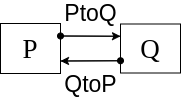
\includegraphics[scale=0.4]{figures/p_and_q.png}
	\caption{Two channels can define capture communication, but provider-client cycles are not allowed in NomosUC.}
	\label{fig:pandq}
	\end{subfigure}
	~ \ \ \ \ 
	\begin{subfigure}{0.6\textwidth}
	\centering
	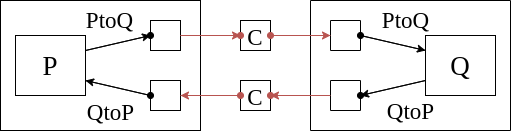
\includegraphics[scale=0.4]{figures/new_p_and_q.png}
	\caption{We can realize the left be intermediating communication with communicators. The direction of messages from $P$ to $Q$ still suggest a cycle but the communicator is provider (dot) to \emph{both} shell codes.}
	\label{fig:newpandq}
	\end{subfigure}
	\caption{Two ITM configurations. One possible with ITMs (left) and one realized in NomosUC (right). Arrows indicate direction of messages and the dot indicates the provider of the channel.}
\end{figure}
Communication between $S_1$ and $S_2$ along channels they each offer results in another cycle. 
Therefore, we break the cycle by intermediating their communication through a \emph{communicator}.
The communicator avoids cycles by offered a \emph{shared channel} rather than the typical linear channel.

\paragraph*{\textbf{Shared Channels}}
\todo{Here I'm not too sure on whether this is enoug information or if it's correct.}
Linear channels are exclusive to the parent and child that are at their endpoints.
Balzer et al.~\cite{balzer2017manifest} proposed a \emph{shared} extension of session types which allows them to capture more natural programming scenarios where cyles naturally occurrs (ring network, dining philosophers, etc.).
Shared channels are still restricted to one provider but can be used by multiple clients to communicate with the provider. 
They introduce non-determinism that isn't present in UC where many clients can be attempting to communciate with the same provider, however, NomosUC borrows the write token from ILC to ensure activation and control are always with only on process at a time.

\paragraph*{\textbf{Communicators}}
Communicators act as channel buffers that two parties can use to communicate to each other.
The shared type of the communicators is given by 
\begin{center}
\parbox{0cm}{
\begin{tabbing}
$\m{comm[a]} = \up \echoice{$\=$\mb{SEND}: \m{a} \product \m \down \m{comm[a]},$\\
\>$\mb{RECV}: \ichoice{$\=$\mb{yes}: \m{a} \product \down \m{comm[a]},$\\
\>\>$\mb{no}: \down \m{comm[a]}}}$
\end{tabbing}}
\end{center}
The $\up$ and $\down$ operations around the session type indicate that it is \emph{shared}, and they denote a \emph{critical section} analogous to traditional concurrency controls like the mutex.
The type suggests that one party can send a message to the communicator, the communicator, buffers the message, and responds with it when asked to \m{RECV} is from a another process.

Returning to the initial example of $P$ and $Q$, although the contruction appears excessive, it is generic and can intermediate communication between any pair of processes in NomosUC. 
It allows us to continue to meaningfully use session types and avoid worrying about cyclical provider/client relationships for the remainder of this paper.
As we show in Section~\ref{sec:execuc}, communicators also help intermediat eocmmunication between each of the main processes of the execution.

\section{The rest of nomos? don't know how to break up this section to include the above.}
\paragraph*{\textbf{Import Tokens}}
A defining aspect of NomosUC is the representation of import tokens in the type system.
This enables a static reasoning of the import mechanism in NomosUC.
To this end, we introduce a novel token context $\Tokens$
in the process typing judgment to denote the real and virtual tokens.
This context contains the information on the total and current tokens
of each type and the \emph{security parameter}.
Before we explain the token context we first motivate the need for virtual tokens
It is a common technique in UC, especially in simulators, to internally run, or simulate, 
the code of other ITIs. In NomosUC, we wish to enable the same sandbox running of processes,
but its channels may have import requirements. It doesn't make sense to
send real import to such a process, because, intuitively the internal process should use the
import and, therefore, potential available to the ``host'' process~\footnote{As far as resource-contraints go, simulating a process should be no different from natively executing its code.}. Therefore, in 
order to satisfy the types of internally simulated processes we introduce a virtual 
tokens construction. 
By default, every process contains a unique real token type $K_0$
and corresponding number of total and current tokens $n$ and $n'$ resp.\
denoted by $K_0 \hookrightarrow (n, n')$.
There is no mechanism to create a real token; they can only be passed on to
a process during its creation, or be exchanged between processes during communication.
Virtual tokens, on the other hand, can be created (under certain conditions,
see below) by a process.
However, all tokens follow a \emph{token hierarchy}: $K_0 \to K_1 \to K_2 \to \ldots K_m$
such that we can only use tokens of type $K_i$ to withdraw tokens of type
$K_{i+1}$~\footnote{ITIs in UC can have arbitrary simulation depth, i.e. a process simulates another process which simulates another process. Despite this, we can statically define the token heirarchy because it is statically known the maximum simulation depth of any process in the UC execution.}.
In addition, we use a global function $\GlobalF$ as the connection
rate between two successive token types.

To maintain well-typedness of a process, an implicit side condition is
that the token context must always be \emph{valid}.
This involves ensuring that if the context contains $m'$ current tokens of type
$K_i$, it can only contain at most $\GlobalF(m,k)$ total tokens of type
$K_{i+1}$. The inductive rules for validity of a token context are below.
\begin{mathpar}
  \infer
  {K_0 \hookrightarrow (t_0, t_0') \;\; \m{valid}}
  {}
  \and
  \infer
  {k \and \Tokens, K_{i+1} \hookrightarrow (t_{i+1}, t_{i+1}')\;\; \m{valid}}
  {\Tokens\;\; \m{valid} \and
  K_{i} \hookrightarrow (t_i, t_i') \in \Tokens \and
  t_{i+1} \leq \GlobalF(t_i',k)}
\end{mathpar}
Since validity of a token context is a side condition, we mandate
that it is implicitly satisfied by all the process typing rules
presented in our paper.
From an implementation point-of-view, this validity check only
needs to be performed when the token context changes (in the
rules that follow).

As a first step in introducing program notation for import tokens, we need 
syntax for creating new tokens of a given token type.
We call this construct $\m{withdrawToken} \; K_i \; n \; K_{i+1}$.
\begin{mathpar}
  \inferrule*[right=$\m{tok}$]
  {k \semi \Tokens, K_{i+1} \hookrightarrow (t_{i+1} + n, t_{i+1}' + n) \semi
  \Psi \semi\wt, \D \entailpot{\B{q}}{\B{q'}} P :: (x : A)}
  {k \semi \Tokens, K_{i+1} \hookrightarrow (t_{i+1}, t_{i+1}') \semi \Psi \semi \wt, \D \entailpot{\B{q}}{\B{q'}} \hspace{4em} \\
    \hspace{5em}\m{withdrawToken} \; K_i \; n\; K_{i+1}  \semi P :: (x : A)}
\end{mathpar}
The above construct generates $n$ new tokens of type $K_{i+1}$ and adds
them to both the total and current count for $K_{i+1}$ in the token
context $\Tokens$.
The implicit side condition of the validity of the token context ensures
that $t_{i+1} + n \leq \GlobalF(t_i',k)$ where $K_i \hookrightarrow (t_i, t_i') \in \Tokens$.
If this side condition fails, the above construct would fail to typecheck.

In addition, we also introduce two dual constructs for exchanging tokens
between processes.
To this end, we first introduce two new type constructors.
\begin{center}
\begin{minipage}{0cm}
\begin{tabbing}
$A ::= \ldots \mid \tpaypot{A}{r : K} \mid \tgetpot{A}{r : K}$
\end{tabbing}
\end{minipage}
\end{center}
The provider of $x : \tgetpot{A}{r : K}$ is required to receive
$r$ import tokens of type $K$ from the client using the construct
$\eget{x}{r : K}$. Dually, the client needs to pay this import
using the construct $\epay{x}{r : K}$.
The corresponding typing rules are
\begin{mathpar}
  \footnotesize
  \infer[\getpot R]
  {k \semi \Tokens, K_i \hookrightarrow (t_i, t_i') \semi \Psi \semi \D \entailpot{\B{q}}{\B{q'}} \eget{x}{r : K_i} \semi P ::
  (x : \tgetpot{A}{r : K_i})}
  {k \semi \Tokens, K_i \hookrightarrow (t_i, t_i'+r) \semi \Psi \semi \wt, \D \entailpot{\B{q}}{\B{q'}} P :: (x : A)}
  %
  \and
  %
  \infer[\getpot L]
  {k \semi \Tokens, K_i \hookrightarrow (t_i, t_i'+r) \semi \Psi \semi \wt, \D, (x : \tgetpot{A}{r : K_i}) \entailpot{\B{q}}{\B{q'}}
  \epay{x}{r : K_i} \semi P :: (z : C)}
  {k \semi \Tokens, K_i \hookrightarrow (t_i, t_i') \semi \Psi \semi \D, (x : A) \entailpot{\B{q}}{\B{q'}} P :: (z : C)}
\end{mathpar}
In the rule $\getpot R$, process $P$ storing $(t_i, t_i')$ import tokens of type $K_i$
receives $r$ additional $K_i$ tokens adding it to the current token counter, thus
the continuation executes with $(t_i, t_i'+r)$ tokens of type $K_i$.
Note that validity of token context is trivially satisfied in this case since the
process is gaining import tokens.
%
In the dual rule $\getpot L$, a process containing $(t_i, t_i'+r)$ tokens of type $K_i$
pays $r$ units along channel $x$ leaving $(t_i, t_i')$ import tokens of type $K_i$ with
the continuation.
In this case, the validity of the token context establishes that $t_{i+1} \leq \GlobalF(t_i',k)$,
a condition that is necessary for successful typechecking.
The typing rules for the dual constructor $\tpaypot{A}{r : K}$
are the exact inverse.
Similar to prior rules, the sender transfers the write token $\wt$
along with the potential to the receiver.

The need for virtual tokens in UC arises because machines often simulate
other machines as part of their construction. The program notation for \msf{withdrawToken}
does not require an inverse to exchange tokens \textit{back} from type $K'$ to $K$.
The reason is that virtual tokens only exist to allow re-use of existing processes 
and satisfy their types. Type $K$ tokens are not deducted when new ones of type $K'$ 
are created is because, in reality, siulating a process by calling it or simply running
its code natively should be equivalent in cost. Therefore, there is also no need to 
include an inverse of \msf{withdrawToken} which exchanges from $K'$ to $K$.

\paragraph*{\textbf{Potential}}
The main purpose of import tokens is to bound the number of execution steps of ITMs.
We achieve that purpose in NomosUC by introducing the notion of \emph{potential}.
Potential is an abstract quantity represented by a natural number stored
within each process.
To take an execution step, a process consumes \emph{one} unit of potential.
Therefore, the total potential stored in a process upper bounds the total
number of execution steps that will ever be taken by the process.
Furthermore, potential is represented syntactically, thus providing a
static upper bound on the execution cost.
Since execution cost needs to eventually connect to the import tokens, all
we need is a mechanism to generate potential using import tokens.
To this end, we introduce a novel construct $\m{genPot} \; r$.
\begin{mathpar}
  \inferrule*[right=$\m{pot}$]
  {q+r \leq \GlobalF(t_{\depth}',k) \and K_{\depth} \hookrightarrow (t_{\depth}, t_{\depth}') \in \Tokens \\\\
  k \semi \Tokens \semi \Psi \semi \wt, \D \entailpot{q+r}{q'+r} P :: (x : A)}
  {k \semi \Tokens \semi \Psi \semi \wt, \D \entailpot{q}{q'} \m{genPot} \; r \semi P :: (x : A)}
\end{mathpar}
A process initially storing $(q, q')$ potential units generates $r$ potential so that
the continuation contains $(q+r, q'+r)$ potential units.
Note, however, that the maximum potential allowed is bounded by the number of import tokens
a process contains.
To this end, we introduce a \emph{token depth}: $\depth$ that signifies the number of token
types that exist in the token hierarchy.
Thus, when generating potential, the typechecker verifies that the total new potential (i.e., $q+r$)
is bounded by $\GlobalF(t_{\depth}',k)$ where $(t_{\depth}, t_{\depth}')$ is the number of tokens
of type $K_{\depth}$, the highest token in the hierarchy.

The purpose of introducing potential into NomosUC is to bound the
number of execution steps.
Therefore, we introduce the $\etick{r}$ construct that consumes $r$
potential from the stored process potential $q$, and the continuation remains with
$p = q-r$ units, as described in the rule below.
\begin{mathpar}
  \footnotesize
  \infer[\m{tick}]
  {k \semi \Tokens \semi \Psi \semi \wt, \D \entailpot{q}{q'+r} \etick{r} \semi P :: (x : A)}
  {k \semi \Tokens \semi \Psi \semi \wt, \D \entailpot{q}{q'} P :: (x : A)}
\end{mathpar}
NomosUC is equipped with a cost instrumentation engine that automatically
inserts a $\etick{1}$ construct before each primitive operation.
This enables us to simulate the cost model that counts the total number of
execution steps.
However, since ticks are not tied directly to the type system, the programmer
can modify the cost model to only count the resource they are interested in
(e.g., message exchange, process spawns, etc.).

% \begin{mathpar}
%   \D_1 \equiv_Z \D_2 \\
%   \D \overset{(import, potential, cost)}{\vDash} P :: \D' \\
%   A \equiv B \\
%   \infer[]
%   {\vars \vdash \D_1, (x : A) \equiv \D_2, (x : B)}
%   {\vars \vdash \D_1 \equiv \D_2 \and \vars \vdash A \equiv B}
% \end{mathpar}

\paragraph*{\textbf{Shared Channels}}
Until now, we have only described the linear fragment of session types
in Nomos.
Unfortunately, this fragment imposes a strong restriction on programs.
The only provision to spawn new processes is when a parent process creates a new
child process, and uses an exclusive linear channel to communicate with the child.
Thus, any two processes connected by a channel inherently maintain this parent-child
relationship.
Intuitively, this leads to a linear tree-like hierarchy among the processes,
thus preventing a cycle in the process graph.

Unfortunately, this restriction precludes practical programming scenarios
where process topologies indeed have a cyclic dependency (e.g. ring networks,
dining philosophers, etc.).
Recognizing this limitation, Balzer et al.~\cite{balzer2017manifest} proposed
a \emph{shared} extension of session types that allows arbitrary process topologies.
The types are extended as follows:
\begin{center}
\begin{minipage}{0cm}
\begin{tabbing}
$A_L ::= \down A_S \mid \ldots \text{(all linear types $A$ so far)}\ldots$\\
$A_S ::= \up A_L$
\end{tabbing}
\end{minipage}
\end{center}
We have found this extension exceedingly helpful in the design and implementation
of cryptographic protocols.

Shared session types impose an \emph{acquire-release} discipline on processes; 
a client must acquire the channel offered by a shared process to interact with it
and must release this channel after the interaction.
The corresponding typing rules are
\begin{mathpar}
  \footnotesize
  \infer[\up L]
  {k \semi \Tokens \semi \Psi \semi \wt, \D, (x : \up A_L)
  \entailpot{q}{q'} \eacquire{y}{x} \semi Q :: (z : C)}
  {k \semi \Tokens \semi \Psi \semi \D, (y : A_L)
  \entailpot{q}{q'} Q :: (z : C)}
  %
  \and
  %
  \infer[\up R]
  {k \semi \Tokens \semi \Psi \semi \D \entailpot{q}{q'}
  \eaccept{y}{x} \semi P :: (x : \up A_L)}
  {k \semi \Tokens \semi \Psi \semi \wt, \D \entailpot{q}{q'} P :: (y : A_L)}
\end{mathpar}
The $\up L$ rule describes a client acquiring a shared channel $x$
and obtaining a private linear channel $y$ along which it can communicate
with the corresponding acquired process.
Correspondingly, the $\up R$ rule describes the shared process
accepting the acquire request and creating the fresh linear channel $y$.
The release-detach rules corresponding to the $\down$ type constructor
are exact dual of acquire-accept.

An important caveat here is that shared channels can introduce non-determinism
in the semantics.
The only source of non-determinism is that a shared process can latch on to
any of the acquiring clients.
To address this problem, we require that the acquiring client \emph{possess
the write token}.
Since write tokens are treated as a linear quantity, only one of the client can
possess it enabling only that process to acquire the shared channel.
Remarkably, this write token can resolve both read and write non-determinism
due to linearity of the channels.


\paragraph*{\textbf{Process Definitions and Sandboxing}}
Process definitions have the form
$\Psi \semi \D \entailpot{q}{q'} f\{\Tokens\} :: (x : A) = P$ where $f$
is the name of the process and $P$ its definition.
We parameterize the process $f$ with the number and type of
real tokens it would need.
All definitions are collected in a fixed global process signature $\Sg$.
Also, since process definitions are mutually recursive, it is required that
for every process in the signature is well-typed w.r.t. $\Sg$.
A new instance of a defined process $f$ can be spawned with
the expression $\procdef{f\{\Tokens\}}{\overline{y}}{x} \semi Q$
where $\overline{y}$ is a sequence of variables matching the
antecedents $\Psi$ and $\D$.
Sometimes a process invocation is a \emph{tail call}, written without
a continuation as $\procdef{f\{\Tokens\}}{\overline{y}}{x}$.
This is a short-hand for
$\procdef{f\{\Tokens\}}{\overline{y}}{x'} \semi \fwd{x}{x'}$ for a
fresh variable $x'$, that is, a fresh channel is created and
immediately identified with $x$.

An important note here is that NomosUC allows executing processes in
a \emph{sandbox}.
Therefore, a process invocation can either be \emph{regular} or in a
\emph{sandbox}.
Syntactically, we use the same term for both but the two invocations
are distinguished via the token type passed into the call.
For a regular call, the parent process passes in a real token type,
while for a sandboxed call, a virtual token type is passed in.
We have a similar distinction for $\m{pay}$ and $\m{get}$ expressions:
if a real token is passed into these terms, it's a regular token
exchange; if a virtual token is passed in, it's a sandboxed $\m{pay}$
and $\m{get}$.

\subsection{Preservation and Progress}
The main type safety theorems that exhibit the deep connection between our type
system and the operational semantics are the usual \emph{type
preservation} and \emph{progress}, sometimes called \emph{session
fidelity} and \emph{deadlock freedom}, respectively.

To exhibit these theorems, we first need to introduce semantic objects
$\proc{c}{w, P}$ and $\msg{c}{w, M}$.
The former (resp. latter) denotes a process (resp. message) executing
expression $P$ (resp. $M$) offering channel $c$ and having performed
work $w$ so far.
The work counter keeps track of execution steps taken by a process,
giving rise to the following semantics rule:
\begin{tabbing}
  $(\m{tick}) : \proc{c}{w, \etick{r} \semi P} \step \proc{c}{w+r, P}$
\end{tabbing}
A multiset of such semantic objects communicating with each other
is known as a \emph{configuration}.
A configuration is typed w.r.t. a signature providing the type declaration
of each process.
A signature $\Sg$ is \emph{well formed} if
(a) every type definition $V = A_V$ is \emph{contractive},
and (b) every process definition
$\Psi \semi \D \vdash f \{\Tokens\} = P :: (x : A)$ in $\Sg$
is well typed according to the process typing judgment, i.e.
$\Tokens \semi \Psi \semi \D \vdash P :: (x : A)$.
 
A key question then is how to type these configurations.
Since they consist of both processes and messages, they
both \emph{use} and \emph{provide} a collection of channels.
Another goal with the type safety theorems is to establish a connection
between the statically determined import tokens of a process,
its total potential, and the dynamically evolving work counters
that account for the total number of execution steps.
We use the following judgment to type a configuration.
\[
\D_1 \overset{(T, Q)}{\underset{W}{\vDash}} \config :: \D_2
\]
It states that the configuration $\config$
uses the channels in the context $\D_1$ and provides the channels in
the context $\D_2$.
In addition, $T$ and $Q$denote the total number of real tokens
potential contained in a configuration.
Similarly, $W$ denotes the total work performed by a configuration.
All these quantities are computed by adding the individual tokens,
potential, and work of each semantic object.
\begin{figure}[t]
\begin{mathpar}
\infer[\m{empty}]
{\D \overset{(0, 0)}{\underset{0}{\vDash}} (\cdot) :: \D}
{}
\and
\infer[\m{compose}]
{\D_0 \overset{(T_1+T_2, Q_1+Q_2)}{\underset{W_1+W_2}{\vDash}} (\config_1 \; \config_2) :: \D_2}
{\D_0 \overset{(T_1, Q_1)}{\underset{W_1}{\vDash}} \config_1 :: \D_1 \qquad
\D_1 \overset{(T_2, Q_2)}{\underset{W_2}{\vDash}} \config_2 :: \D_2}
\and
\infer[\m{proc}]
{\D, \D_1 \overset{(t, q)}{\underset{w}{\vDash}} \proc{c}{w, P} :: (\D, (c : A) )}
{\Tokens, K_0 \hookrightarrow t \semi \cdot \semi \D_1 \entailpot{q} P :: (c : A)}
\and
\infer[\m{msg}]
{\D, \D_1 \overset{(t, q)}{\underset{w}{\vDash}} \msg{c}{w, M} :: (\D, (c : A) )}
{\Tokens, K_0 \hookrightarrow t \semi \cdot \semi \D_1 \entailpot{q} M :: (c : A)}
\end{mathpar}
\caption{Typing rules for a configuration}
\label{fig:config_typing}
\end{figure}

The configuration typing judgment is defined using
the rules presented in Figure~\ref{fig:config_typing}.
%
The rule $\m{empty}$ defines that an empty configuration
is well-typed with $(T, Q, W) = (0, 0, 0)$ and uses and
provides the same set of channels.
The $\m{compose}$ rule combines two configurations by canceling out
the common channels and adding the individual tokens, potential, and work.
The $\m{proc}$ rule creates a configuration out of a single process
and uses its tokens, potential, and work as the annotations for the
configuration.
Similarly, the $\m{msg}$ rule creates a configuration out of a single message.

\begin{theorem}[Type Preservation]
\label{thm:preservation}
Suppose we have a well-typed configuration
$\D \overset{(T_1, Q_1)}{\underset{W_1}{\vDash}} \config_1 :: \D'$ such
that there exists a polynomial $\mathfrak{p}$ such that $\mathfrak{p}(T_1) \geq Q_1+W_1$.
If $\config_1 \step \config_2$, then there exist $T_2$, $Q_2$, and $W_2$ such
that $\D \overset{(T_2, Q_2)}{\underset{W_2}{\vDash}} \config_2 :: \D'$,
and $\mathfrak{p}(T_2) \geq Q_2+W_2$.
\end{theorem}
\begin{proof}
  By case analysis on the transition rule, applying inversion to the
  given typing derivation, and then assembling a new derivation of
  $\dc$.
\end{proof}

A process or message is said to be \emph{poised} if it is trying to
communicate along the channel that it provides.  A poised process is
comparable to a value in a sequential language. A configuration is
poised if every process or message in the configuration is poised.
Conceptually, this implies that the configuration is trying to communicate
externally, i.e. along one of the channel it provides.
The progress theorem then shows that either a configuration can take a
step or it is poised.  To prove this I show first that the typing
derivation can be rearranged to go strictly from right to left and
then proceed by induction over this particular derivation.

\begin{theorem}[Global Progress]
\label{thm:progress}
\mbox{}
If $\cdot \overset{(T, Q)}{\underset{W}{\vDash}} \config :: \D$ then either
\begin{enumerate}
\item[(i)] $\config \mapsto \config'$ for some $\config'$, or
\item[(ii)] $\config$ is poised.
\end{enumerate}
\end{theorem}
\begin{proof}
By induction on the right-to-left typing of $\config$ so that either
$\config$ is empty (and therefore poised) or
$\config = (\dc\; \proc{c}{w, P})$ or
$\config = (\dc\; \msg{c}{w, M})$. By induction hypothesis, $\dc$ can
either take a step (and then so can $\config$), or $\dc$ is poised.  In
the latter case, I
analyze the cases for $P$ and $M$, applying multiple steps of
inversion to show that in each
case either $\config$ can take a step or is poised.
\end{proof}


%\subsection{UC Communicators} \label{sec:communicators}
%% all the processes conncted together leads to a cycle of linear channels ==> Z <--> P so here we use a communicator 
%The UC execution connects the protocol to the environment in both directions of communication.
%This poses a technical challenge where, if linear channels are used, the resulting topology contains a cycle of linear channels: the environmtne offers a channel to the wrapper and the wrapper to the environment.
%Such cycles violate type preservation because a client is acquiring its client~\ref{dasnomos}.
%Therefore, we use a message buffers called communicators which offered shared channels that both ends of the communication can use.
%Communicators are used in the main UC execution in Section~\ref{sec:execuc} to connect the main processes together, as well as within the \partywrapper. 
%
%A communicator has a \emph{sender} and a \emph{receiver}. 
%The shared channel offered by the communicator has the following polymorphic session type:
%\begin{tabbing}
%  $\mi{stype} \; \m{comm[K][msg]\{n\}} =$\\
%  \quad $\up \tgetpot{}{n+1: K} \echoice{$\=$\mb{push} : \m{msg} \arrow
%  \down \m{comm[msg]},$\\
%  \>$\mb{pop} : \ichoice{$\=$\mb{yesmsg} : \m{msg} \product \down \tpaypot{}{n: K} \m{comm[msg]},$\\
%  \>\>$\mb{nomsg} : \down \m{comm[msg]} }}$
%\end{tabbing}
%
%One illustration of the use of shared session types is a \emph{communicator}.
%We use communicators as message buffers between two arbitrary processes: a
%\emph{sender} and a \emph{receiver}.
%The communicator is connected to both the sender and the receiver using a shared
%channel.
%
%Intuitively, the communicator receives \emph{push} requests from the sender followed
%by receiving a message and stores them internally.
%Analogously, the communicator receives \emph{pop} requests from the receiver,
%and responds appropriately with the message if one is stored inside the communicator.
%Formally, a communicator has the following polymorphic session type
%\begin{tabbing}
%  $\mi{stype} \; \m{comm[K][msg]\{n\}} =$\\
%  \quad $\up \tgetpot{}{n+1: K} \echoice{$\=$\mb{SEND} : \m{msg} \arrow
%  \down \m{comm[msg]},$\\
%  \>$\mb{RECV} : \ichoice{$\=$\mb{yes} : \m{msg} \product \down \tpaypot{}{n: K} \m{comm[msg]},$\\
%  \>\>$\mb{no} : \down \m{comm[msg]} }}$
%\end{tabbing}
%The $\up$ indicates that it is a shared channel that must be \emph{acquired} by a process in order to send something over it.
%
%The sender can $\mb{SEND}$ a message into the communicator, and the receiver can periodically try to $\mb{RECV}$ a message from it.
%If there is a message, it responds with $\mb{yes}$, the message of the parameterized type $\m{msg}$, and the import sent with it.
%Note that the communicator retains one unit of import from every message. 
%It needs at least one because it may be activated a polynomial number of times, and, therefore a constant amount of potential is insufficient. 
%At the end of activation, the channel is released with $\down$, and another process can acquire it.

\subsection{Discussion on Realizing Import}
Our adaptation of the import mechanism to resource-aware session types concretizes some parts of the import mechanism like the run-time budget and adds new mechanisms
to facilitate common UC design pattersn such as simulation and virtualization of machines. 
It's important to validate our realization of the import mechanism by ensuring that it faithfully provides the same guarantees.
Furthermore, in this section we discuss existing pitfalls and drawbacks of prior mechanisms that import was created to over come, and assert that our implementation steers clear of them as well.

An important part of our discussion must focus around our sandboxing technique and ensuring that it does not provide a pathway for a process to run infinitely.
The infinite runs problems is a persistent issue in existing length-of-input based approaches to polynoimal time.
It naturally appears in our sandboxing mechanism by the continual creation of new virtual token types. Following from the intent of sandboxing, the NomosUC rule for a valid token context ensures that all virtual token types  \todo{ finish this by deciding which rule to update: \inline{genPot} or \inline{withdrawTokens}}

%\begin{itemize}
%\item Identify design decisions like concretizing potential, sandboxing and virtualizing with withdrawTokens, the valid token context rule, the type system in general
%\item Identify polytime concerns that need to be discussed in the context of our polytime design
%	\begin{itemize}
%	\item is PPT efficiently recognizable?
%	\item address the infinite runs problem and make sure it isn't allowed here with particular attention paid to withdrawTokens and infinite virtualizations
%	\item the type system guarantees we don't have a case where, given some polynomial, a machine just halts mid execution so we avoid any additional information that an environment can use to distinguish based on execution timing in both word
%	\end{itemize}
%\item end with the virtualization point and tie that into proposition 7 and the universal turing machine that can simulate the UC execution. This goes a long way in assuring PPT notion in NomosUC, even thought we aren't dealing exactly with ITMs here.
%\end{itemize}

%The type $\m{comm}$ is parameterized by the type $\m{msg}$, i.e., the type of
%messages in the buffer, and import type parameter, i.e. the amount of import tokens sent with
%the message. 
%The type initiates with an $\up$ denoting that $\m{comm}$ is a shared session type.
%The type prescribes that the communicator needs to be acquired by the sender (or receiver)
%for further interaction.
%Such an acquire-release discipline is automatically enforced by the shared session type.
%Once acquired, the communicator can either receive $\mb{push}$ (from sender) or
%$\mb{pop}$ requests (from receiver).
%In the former case, the communicator receives a message of type $\m{msg}$ and $n+1:K$ import tokens, and
%then detaches from the client using the dual $\down$ operator.
%In the latter case, the communicator checks if it internally contains a message
%for the receiver.
%If yes, the communicator replies with the $\mb{yesmsg}$ label followed by sending
%the message (the $\product$ constructor) and $n:K$ import tokens.
%Otherwise, the communicator replies with the $\mb{nomsg}$ label.
%In either case, the communicator then detaches from the client matching the $\down$
%operator.
%Internally, the communicator stores these messages in a first-in-first-out order.

%It is important to note that our communicators need at least 1 token of import 
%to use themselves to handle a potentially polynomial number of activations. 
%Therefore, it requires $n+1$ units of import from the sender and sends the intended
%$n$ tokens to the receiver when requested.

%The communicator is also the perfect opportunity to implement an unreliable
%message buffer that can drop or reorder messages.
%All we would need to do is change the internal implementation of the communicator
%\emph{without} changing the offered session type.


\section{Selected Typing Rules for NomosUC} \label{app:typing_rules}
\paragraph*{\textbf{Choice Operators}}
The internal choice $\ichoice{\ell : A_\ell}_{\ell \in L}$ constructor
is an $n$-ary labeled generalization of the additive disjunction $A \oplus B$.
A process that provides $x : \ichoice{\ell : A_\ell}_{\ell \in L}$ can send
any label $k \in L$ along $x$ and then continue by providing $x : A_k$. The
corresponding process is written as $(\esendl{x}{k} \semi P)$, where
$P$ is the continuation that provides $A_k$.
On the other end of the channel, the client branches on the label received along $x$.
The provider and client are typed according to the following $\oplus R$ and $\oplus L$
rules respectively.
\begin{mathpar}
  \infer[{\oplus}R]
  {\B{\Tokens \semi \Psi} \semi \wt, \D \entailpot{\B{q}}{\B{q'}} (\esendl{x}{k} \semi P) ::
    (x : \ichoice{\ell : A_\ell}_{\ell \in L})}
  {(k \in L) \qquad \B{\Tokens \semi \Psi} \semi \D \entailpot{\B{q}}{\B{q'}} P :: (x : A_k)}
\and
  \infer[{\oplus}L]
  {\B{\Tokens \semi \Psi} \semi \D, (x : \ichoice{\ell : A_\ell}_{\ell \in L})
    \entailpot{\B{q}}{\B{q'}} \ecase{x}{\ell}{Q_\ell}_{\ell \in L} :: (z : C)}
  {(\forall \ell \in L) \qquad \B{\Tokens \semi \Psi} \semi \wt, \D, (x : A_\ell)
    \entailpot{\B{q}}{\B{q'}} Q_\ell :: (z : C)}
\end{mathpar}
Additionally, the provider should possess the write token to be able to send the
label $k$. Dually, the client receives the write token with the label to continue
execution.

Operationally, since communication is asynchronous, the process
$(\esendl{c}{k} \semi P)$ sends a message $k$
along $c$ and continues as $P$ without waiting for it to be received.
As a technical device to ensure that consecutive messages on a
channel arrive in order, the sender also creates a fresh continuation
channel $c'$ so that the message $k$ is actually represented as
$(\esendl{c}{k} \semi \fwd{c}{c'})$ (read: send $k$ along $c$ and
continue as $c'$). The provider substitutes $c'$ for $c$ enforcing
that the next message is sent on $c'$.
The work counter of the process remains unaltered, and the new message
is created with work $0$.
\begin{tabbing}
$(\oplus S) : \proc{c}{w, \esendl{c}{k} \semi P} \step \proc{c'}{w, [c'/c]P},
\msg{c}{0, \esendl{c}{k} \semi \fwd{c}{c'}} \qquad \qquad \fresh{c'}$
\end{tabbing}
When the message $k$ is received along $c$, the client selects branch
$k$ and also substitutes the continuation channel $c'$ for $c$, thereby
ensuring that it receives the next message on $c'$. This implicit
substitution of the continuation channel ensures the ordering of the
messages.
The client process also collects the work performed by the message, if
there is any.
\begin{tabbing}
$(\oplus C) :$ \= $\msg{c}{w, \esendl{c}{k} \semi \fwd{c}{c'}},
\proc{d}{w', \ecase{c}{\ell}{Q_\ell}}
\step \proc{d}{w+w',[c'/c]Q_k}$
\end{tabbing}

The dual of internal choice is \emph{external choice} $\echoice{\ell :
A_\ell}_{\ell \in L}$, the $n$-ary labeled generalization of the
additive conjunction $A \with B$. This dual operator simply reverses
the role of the provider and client. The provider process of
$x : \echoice{\ell : A_\ell}_{\ell \in L}$ branches on receiving a label
using the expression $\ecase{x}{\ell}{Q_\ell}_{\ell \in L}$,
while the client sends one such label in $L$ using the expression $(\esendl{x}{k} \semi P)$.

\begin{mathpar}
  \infer[\with R]
  {\B{\Tokens \semi \Psi} \semi \D \entailpot{\B{q}}{\B{q'}} \ecase{x}{\ell}{P_\ell}_{\ell \in L} ::
    (x : \echoice{\ell : A_\ell}_{\ell \in L})}
  {(\forall \ell \in L) \qquad \B{\Tokens \semi \Psi} \semi \wt, \D
    \entailpot{\B{q}}{\B{q'}} P_\ell :: (x : A_\ell)}
\and
  \infer[\with L]
  {\B{\Tokens \semi \Psi} \semi \wt, \D, (x : \echoice{\ell : A_\ell}_{\ell \in L})
    \entailpot{\B{q}}{\B{q'}} \esendl{x}{k} \semi Q :: (z : C)}
  {\B{\Tokens \semi \Psi} \semi \D, (x : A_k) \entailpot{\B{q}}{\B{q'}} Q :: (z : C)}
\end{mathpar}
Dual to internal choice, the client contains the write token which is
sent to the provider along with the label.

The provider receives the branching label $k$ sent by the provider. Both
processes perform appropriate substitutions to ensure the order of messages
sent and received is preserved.
\[
\begin{array}{lll}
(\with S) & \proc{d}{w, \esendl{c}{k} \semi Q} \step \msg{c'}{0, \esendl{c}{k}
\semi \fwd{c'}{c}}, \proc{d}{w, [c'/c]Q} \qquad \fresh{c'} \\
(\with C) & \proc{c}{w, \ecase{c}{\ell}{Q_\ell}_{\ell \in L}},
\msg{c'}{w', \esendl{c}{k} \semi \fwd{c'}{c}} \step \proc{c'}{w+w', [c'/c]Q_k}
\end{array}
\]

\paragraph*{\textbf{Termination}}
The type $\one$, the multiplicative unit of linear logic, represents
termination of a process, which is not allowed to use
any linear channels. A terminating process offering on $x : \one$ simply
closes channel $x$ using the expression $\eclose{x}$ while the client waits
for this close message to arrive using the expression $\ewait{x} \semi Q$
and then continues executing $Q$.
\begin{mathpar}
  \infer[{\one}R]
  {\B{k \semi \Tokens \semi \Psi} \semi \wt \entailpot{\B{q}}{\B{q'}} \eclose{x} :: (x : \one)}
  {\B{q = 0}}
  \and
  \infer[{\one}L]
  {\B{k \semi \Tokens \semi \Psi} \semi \D, (x : \one) \entailpot{\B{q}}{\B{q'}} (\ewait{x} \semi Q) :: (z : C)}
  {\B{k \semi \Tokens \semi \Psi} \semi \wt, \D \entailpot{\B{q}}{\B{q'}} Q :: (z : C)}
\end{mathpar}
Similar to internal choice, the closing process transfers the write
token to its waiting client along with the close message.
Additionally, the terminating process does not store
any potential since it cannot take any further execution steps
(explained more in Section~\ref{sec:import}).

Operationally, the provider converts into a closing message
with no continuation since the offered channel terminates.
\begin{tabbing}
$(\one S) : \proc{c}{w, \eclose{c}} \step \msg{c}{w, \eclose{c}}$ \\
$(\one C) : \msg{c}{w, \eclose{c}}, \proc{d}{w'\ewait{c} \semi Q} \step
\proc{d}{w+w', Q}$
\end{tabbing}



\paragraph*{\textbf{Exchanging Functional Data}}
So far, we have discussed the channels in $\D$ in the typing judgment for NomosUC.
Now, we turn out attention to the functional layer $\Psi$ that contains the
traditional data structures and values.
Communicating a \emph{value} of the functional fragment along a channel
is expressed at the type level by adding the following two session types.
\begin{center}
\begin{minipage}{0cm}
\begin{tabbing}
$A ::= \ldots \mid \tau \arrow A \mid \tau \product A$
\end{tabbing}
\end{minipage}
\end{center}
Here, $\tau$ describes a functional type, e.g. $\m{int}, \m{bool}, \tau \; \m{list}$, etc
(we assume the language contains standard functional types).
The type $\tau \arrow A$ prescribes receiving a value of type $\tau$
with continuation type $A$, while its dual $\tau \product A$ prescribes
sending a value of type $\tau$ with continuation $A$. The corresponding
typing rules for arrow ($\arrow R, \arrow L$) are given below.
\begin{mathpar}
  \infer[\arrow R]
  {\B{\Tokens} \semi \Psi \semi \D \entailpot{\B{q}}{\B{q'}}
  \erecvch{x}{v} \semi P :: (x : \tau \arrow A)}
  {\B{\Tokens} \semi \Psi, (v : \tau) \semi \wt, \D \entailpot{\B{q}}{\B{q'}}
  P :: (x : A)}
  %
  \and
  %
  \inferrule*[right = $\arrow L$]
  {\B{r' = p+q'} \qquad
  \B{\Psi \share (\Psi_1, \Psi_2)} \qquad
  \Psi_1 \exppot{\B{p}} M : \tau \\
  \B{\Tokens} \semi \Psi_2 \semi \D, (x : A) \entailpot{\B{q}}{\B{q'}}
  Q :: (z_k : C)}
  {\B{\Tokens} \semi \Psi \semi \wt, \D, (x : \tau \arrow A)
  \entailpot{\B{q}}{\B{r'}} \esendch{x}{M} \semi Q :: (z : C)}
\end{mathpar}
As indicated in the $\arrow R$ rule, receiving a value $y : \tau$ on a channel
$x : \tau \arrow A$ adds it to the functional context $\Psi$. On the
other hand, sending (value of) expression $M$ on channel $x : \tau \arrow A$
requires that $M$ has type $\tau$ (third premise).
The premises indicated in blue describe how potential is divided across
the functional and session-typed layers and will be described further in Section~\ref{sec:import}.
Intuitively, the potential in functional context $\Psi$ is \emph{shared}
between $\Psi_1$ and $\Psi_2$ (second premise); $\Psi_1$ is used to type
$M$ while $\Psi_2$ is passed on to the continuation $Q$.
The $\product$ operator is dual to $\arrow$ reversing the roles of provider and client,
and we omit those rules for brevity.



\paragraph*{\textbf{Shared Channels}}
Shared session types impose an \emph{acquire-release} discipline on processes; 
a client must acquire the channel offered by a shared process to interact with it
and must release this channel after the interaction.
The corresponding typing rules are
\begin{mathpar}
  \infer[\up L]
  {\Tokens \semi \Psi \semi \wt, \D, (x : \up A_L)
  \entailpot{q}{q'} \eacquire{y}{x} \semi Q :: (z : C)}
  {\Tokens \semi \Psi \semi \D, (y : A_L)
  \entailpot{q}{q'} Q :: (z : C)}
  %
  \and
  %
  \infer[\up R]
  {\Tokens \semi \Psi \semi \D \entailpot{q}{q'}
  \eaccept{y}{x} \semi P :: (x : \up A_L)}
  {\Tokens \semi \Psi \semi \wt, \D \entailpot{q}{q'} P :: (y : A_L)}
\end{mathpar}
The $\up L$ rule describes a client acquiring a shared channel $x$
and obtaining a private linear channel $y$ along which it can communicate
with the corresponding acquired process.
Correspondingly, the $\up R$ rule describes the shared process
accepting the acquire request and creating the fresh linear channel $y$.
The release-detach rules corresponding to the $\down$ type constructor
are exact dual of acquire-accept.


\section{Arbitrary Parties} \label{app:arbparties}

The example we've used throughout this paper, \Fcom, supports only a limited number of parties.
We realize the functionality, in Section~\ref{sec:commitment}, with a protocol that uses random oracle \Fro--an idealize hash function.
This functionality allows for an arbitrary number of parties to write to it, and is the first example so far that makes use of the arbitrary parties support.
An environment that uses our arbitrary party mechanism is shown in Figure~\ref{fig:envarb}.

\begin{figure}
	\centering
	\begin{lstlisting}[basicstyle=\footnotesize\BeraMonottFamily, mathescape, frame=single]
$\nproc$ env_ro[K] :
  (k: Int), (rng: [Bit]), (sid: session[a]),
  (#z_to_pw: comm[z2pmsg[rop2f]]), (#pw_to_z: comm[p2zmsg[rof2p]]),
  (#z_to_a: comm[z2amsg[roa2f]]), (#a_to_a: comm[a2zmsg[roz2a]]) |- (#ch: EtoZ[a]) =
{
  ...
  b <- $\yo{sample}$ rng 5 ;
  i = 0 
  $\nwhile$ i < b {
    p <- $\tb{sample}$ rng k ;
    #z_to_pw.SEND ;
    $\tg{(* each call spawns a new party with pid=i *)}$
    $\nsend$ #z_to_pw Z2P(i, QHash(p)) ;
    ...
  }
  $\$$ch.output ;
  $\nsend$ $\$$ch 1 ;
}
	\end{lstlisting}
	\caption{An example of an environment that spawns an arbitrary number of parties. For the sake of clarity we present this example without the use of any import.}
	\label{fig:envarb}
\end{figure}

The environment is well-matched with an execution where dummy parties are used, parties the forward messages from \Z (or \A if they are corrupt) to the functionality, and does the same to messages from \F to \Z.
    	


\section{Dummy Lemma} \label{app:dummy}
\subsection{Dummy Lemma} \label{sec:dummy}
The dummy lemma is a crucial result in UC that reduces the design space of simulators to just one: the one for the dummy adversary in the real world.
The Lemma presents the construction of a simulator from the \DS for any adversary \A. Our constructed Dummy Lemma simulator uses virtual tokens to simulate \DS and \A internall and route messages between them.
At a high level the Lemma asserts that an execution with \DS and the dummy adversary must work for all environments even those running some \A internally.
If the \A moves from \Z into the real world execution as th real adverasry and the ideal world connected to \DS then the emulation must still hold.

A proof of the dummy lemma relies on creating a simulator \Sim for an arbitrary adversary given \DS.
Recall from the original discussion in Section~\ref{sec:dummy} that the intuition behind the Dummy Lemma can be seen from the basic definition of emulation.

Consider UC emulation with respect to the dummy adversary. The emulation definition quantifies over all environments. 
This includes an environment that runs any arbitrary real-world adversary \A, for the protocol, internally, and \Z forwards the outputs from the adversary to the dummy adversary and dummy simulator in the execution.
Consider the modified execution where \A is run in the real execution instead of internally: it is the adversary in the real world and it is run as part of the simulator in the ideal world.
The ideal world simulator runs \A and the dummy sim internally and passes input from \Z to \A and output from \A to \DS.
Moving ITMs from inside \Z to the real world is a common pattern in UC proofs and is used in the composition proof as well.
We depict the intuition in Figure~\ref{fig:dummylemmas}.

\begin{figure}[t!]
	\begin{subfigure}[t]{0.2\textwidth}
	\centering
	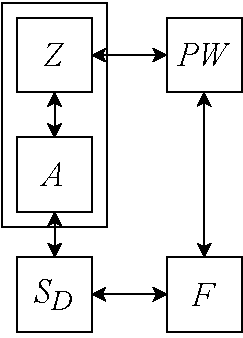
\includegraphics[scale=0.5]{figures/dummylemma_pre.pdf}
	\caption{An environment running \A internally is captured by the $\forall$ quantifier for the emulation definition with respect to the dummy adversary.}
	\label{fig:dummy_pre}
	\end{subfigure}
	~
	\begin{subfigure}[t]{0.2\textwidth}
	\centering
	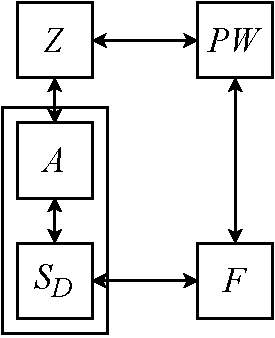
\includegraphics[scale=0.5]{figures/dummylemma_post.pdf}
	\caption{Moving the adverary out of \Z and into the execution results in the same inputs to the protocol and functionalities in both worlds and hence we expect emulation to hold.}
	\label{fig:dummy_post}
	\end{subfigure}
	\caption{Graphical illustration of the intuition behind the Dummy Lemma.}
	\label{fig:dummylemmas}
\end{figure}


We restate the Dummy Lemma here:
\begin{theorem}[Dummy Lemma]\label{thm:dummy}
If \ $\exists \DS$ s.t. $ \DA, \DS \vdash \F_2 \xrightarrow{\pi} \F_1$ then $\forall \A \ \exists \Sim_\A$ s.t. $\Sim_{\A} \vdash  \F_2 \xrightarrow{\pi} \F_1)$ 
\end{theorem}

\begin{proof}
The constructed simulator $\Sim_\A$ runs \A and \DS internally.
$\Sim_\A$ sandboxes the two simulators using our virtual tokens construction.
The construction simulator is straightforward, and we provide sample snippets of code from the simulator.
The adversaries \A and \DS expect to receive input from \Z through communicator.

The simulator creates channels for each of \A and \DS and connects them together.
For example, output from \A on its channel to a party or the functionality is merged 
into input from \Z for \DS.
In the dummy simulator the channels are created as:
\begin{lstlisting}[basicstyle=\footnotesize\BeraMonottFamily, frame=single,  mathescape]
$\$$a2ps <- channel_init[K1][p2f] ;
$\$$a2fs <- channel_init[K1][s2f] ;
$\$$z2s <- channl_init[K1][Z2A[p2f][s2f]] ;
<- a2z_wrap[K][p2f][s2f] <- $\$$a2ps $\$$a2fs $\$$z2s ;
\end{lstlisting}
where \inline{a2z_wrap} simply reads from \inline{$\$$a2ps} and \inline{$\$$a2fs} and wraps it in the type constructor for messages from \Z to \A:
\begin{lstlisting}[basicstyle=\footnotesize\BeraMonottFamily, frame=single,  mathescape]
$\nproc$ a2s_wrap[K][a][b]{an,bn,dsn}:
  ($\$$in2p: a2p[K][a]{an}), ($\$$in2f: a2f[K][b]{bn}), 
  ($\$$out: z2a[K][Z2A[a][b]]{dsn}) |- ($\$$c : 1) =
{
  $\nmatch$ $\$$in2p, $\$$in2f (
    *,A2F => m = $\nrecv$ $\$$in2f ; 
	$\nget$ K {bn} $\$$in2f ;
	$\$$out.Z2A2F ; $\nsend$ $\$$out m ;
	$\npay$ K {dsn} $\$$out ;
    A2P,* => (pid,m) = $\nrecv$ $\$$in2p ;
	$\nget$ K {an} $\$$in2p ;
	$\$$out.Z2A2P ; $\nsend$ $\$$out (pid,m) ;
	$\npay$ K {fsn} $\$$out ;
  )
  $\tg{(* proceed to next reads *)}$
}
\end{lstlisting}

On input from \Z, we simply forward the message with virtual tokens instead of real tokens and outgoing messages from \A as real output to \Z:
\begin{lstlisting}[basicstyle=\footnotesize\BeraMonottFamily, frame=single,  mathescape]
$\nmatch$ $\$$z2a, $\$$a2z' (
  Z2A2P,* => (pid,m) = $\nrecv$ $\$$z2a ;
  	$\nget$ K {z2an} $\$$z2a' ;
    $\nwithdraw$ K K1 {z2an} ;
    #z2a'.Z2A2P; $\nsend$ $\$$z2a' (pid, m);
    $\npay$ K1 {z2an} $\$$z2a' ;
  Z2A2F,*=> m = $\nrecv$ $\$$z2a' ;
  	$\nget$ K {z2an} $\$$z2a' ;
    $\nwithdraw$ K K1 {z2an} ;
    $\$$z2a'.Z2A2F; $\nsend$ $\$$z2a' m ;
    $\npay$ K1 {z2an} $\$$z2a' ;
  $\tg{(* identical in the reverse *)}$
)
\end{lstlisting}
We use the \inline{match} over shared channels as syntax sugar that abstracts away their special handling and receiving the given import and token type from them. 

Input from the ideal world \F or the \partywrapper is forwarded, virtualy, to \DS in the same way as above. 
\end{proof}


\section{Multisession Theorems} \label{app:ms}
In this section we give more extensive code on how themultisession extension work. We also exlore Theorems \ref{thm:squash} and \ref{thm:functor} in greater detail, and, specifically address the proof obligation for both.

\subsection{!\F}
The multisession operator presents the same interface to \inline{execUC} as any other functionality.
However, the shell code that we run it inside operates directly on functional messages from its communicators with \F and the \partywrapper instead of performing any conversion to session-types.
The reason for this choice is that a session type for the operator is not very meaningful as it only provides an interface of ``input'' and ``ouput'' to/from underlying instances of the functionality.

!\F communicates with the \partywrapper through the type
\begin{lstlisting}[basicstyle=\small\BeraMonottFamily, mathescape]
$\yo{type}$ p2ms[a] = P2MS of ssid ^ a ;
$\yo{type}$ ms2p[b] = MS2P of ssid ^ b ;
\end{lstlisting}
and with \A through the type
\begin{lstlisting}[basicstyle=\small\BeraMonottFamily, mathescape]
$\yo{type}$ a2ms[a] = A2MS of ssid ^ a ;
$\yo{type}$ ms2a[b] = MS2A of ssid ^ b ;
\end{lstlisting}
both of which are parameterized by the functionality message types \inline{a} and \inline{b}.


Recall that all functionalities are run inside some shell code, and their shell code communicates with communicators to other parities--we can call this a functionality wrapper as it wraps around the actual functionality code.
The multisession operator runs each instance of the functionaly inside the wrapper, and provides each with ``virtual'' communicators for \A and the \partywrapper.

The !\F, on input from the \partywrapper, reads a message from the communicator and then does the following:
\begin{lstlisting}[basicstyle=\footnotesize\BeraMonottFamily, frame=single, mathescape, numbers=left]
$\nproc$ f_multisession_p2f_input[K][K1]{p2fn,f2pn} : 
  (k: Int), (rng: [Bit]), (sid: session[a]), (crupt: list[pid]),
  (#p2f: comm[p2fmsg[p2ms]][K]), (#f2p: comm[f2pmsg[ms2p]][K]), 
  (#a2f: comm[a2fmsg[a2ms]][K]), (#f2a: comm[f2amsg[ms2a]][K]) |- ($\$$ch: 1) =
{
  ...
  msg = $\nrecv$ #p2f ;
  $\ncase$ msg (
    P2F(pid, P2MS(ssid, msg)) =>
      $\nif$ not ssid in $\$$p2ssid
      $\nthen$
      	#new_p2ssid <- communicator_init[K1][p2f] <- ;
      	#new_ssid2p <- communicator_init[K1][f2p] <- ;
      	#new_a2ssid <- communicator_init[K1][a2f] <- ;
      	#new_ssid2a <- communicator_init[K1][f2a] <- ;
      
      	$\$$p2ssidnew <- pappend $\$$p2ssid #new_p2ssid ;
      	$\$$ssid2pnew <- pappend $\$$ssid2p #new_ssid2p ;
      	$\$$a2ssidnew <- pappend $\$$a2ssid #new_a2ssid ;
      	$\$$ssid2anew <- pappend $\$$ssid2a #new_ssid2a ;
      
      	$\$$chprime <- f_wrapper[K1][f2p,p2f][f2a,a2f] <- 
                           k rng sid clist $\#$p2ssid $\#$ssid2p $\#$a2ssid $\#$ssid2a $\#$z ;
      $\nend$
  
      #ch <- get_channel #p2ssid ssid ;
      $\nwithdraw$ K K1 {p2fn} ;
      $\$$ch.SEND ;
      $\nsend$ $\$$ch P2F(pid, msg) ;
      $\npay$ $\$$ch {p2fn : K1} ;
  	
    $\$$ch <- f_multisession_f2p_i[K][K1] <- .... $\$$p2ssidnew $\$$ssid2pnew $\$$a2ssidnew $\$$ssid2anew 0;	
}
\end{lstlisting}

First it checks whether the \m{ssid} exists. It not it spawns new communcators for the instance \F: two for the \partywrapper and two for \A.
It then grabs the \inline{#p2f} channel for $\F_{\m{ssid}}$, creates the appropriate virtual tokens and sends the message along that channel.
Finally, after handling the incoming message, it moves to the next step of checking for outgoing messages, to the \partywrapper, from each \F by calling \inline{f_multisession_f2p_i}.
The function accepts an integer at the end, in this example 0, which is the index to check in the communicator list. Eventually all communicators in the list are checked.

Recall that the Theorem~\ref{sec:squash} realizes !!\F, a functionality wrapped twice in the multisession operator an indexed by a pair of ssids $(\m{ssid}_1 \product \m{ssid}_2)$.
The real world that realizes it is comprised of a protocol that ``flattens'' the pair of ssids $(\m{ssid}_1, \m{ssid}_2)$ into a single ssid $\m{ssid}_3 = \m{ssid}_1 || \m{ssid}_2$, the concatenation (can be any other one-to-one and invertible function on the pair) of them.
The simulator for this construction is a direct simulation where $\Sim{\m{squash}}$ takes as input one of 
\begin{itemize}
	\item \inline{Z2A2P(pid, P2MS(ssid, msg))}: $\SIM{\m{squash}}$ un-concatenates \inline{ssid} into a pair (\inline{ssid1}, \inline{ssid2}) and forward the message \inline{A2P(pid, P2MS(ssid1, P2MS(ssid2, msg)))}.
	\item \inline{Z2A2F(A2MS(ssid, msg))}: Similar to above, $\SIM{\m{squash}}$ splits the given \inline{ssid} and sends \\ \inline{A2F(A2MS(ssid1, A2MS(ssid2, msg)))}. 
\end{itemize}

\SIM{\m{squash}} also keeps one import for every message it ges and forwards the remainder to either of \F or the \partywrapper.
On input from \Z, \SIM{\m{squash}} does the following; 

\begin{lstlisting}[basicstyle=\footnotesize\BeraMonottFamily, frame=single, mathescape]
proc sim_squash[K][p2f,f2p,a2f,f2a]{p2fn,f2pn,a2fn} :
  (k: Int), (rng: [Bit]), (sid: session[a]), (crupt: list[pid]),
  (#z_to_a: comm[z2amsg]), (#a_to_z: comm[a2zmsg]) ... |- ($\$$ch: 1) =
{
  ...
  $\ncase$ #z_to_a (
    Z2A2P(pid, P2MS(ssid, msg))) =>
      ssid1, ssid2 <- split ssid
      #a_to_p.SEND ;
      $\npay$ #a_to_p {a2pn-1} ;
      $\nsend$ #a_to_p A2P(pid, P2MS(ssid2, P2MS(ssid2, msg)) ;
    Z2A2F(A2MS(ssid, msg)) =>
      ssid1,ssid2 <- split ssid
      #a_to_f.SEND ; 
      $\npay$ #a_to_f {a2fn-1} ;
	  $\nsend$ #a_to_f A2P(A2MS(ssid1, A2MS(ssid2, msg))) ;
  ...
}	  
\end{lstlisting}


\section{Commitment Protocol} \label{app:protcom}
In this section we expand on the real world protocol that realizes \Fcom in the \Fropp-hybrid model.
The type of \Fropp in Figure~\ref{fig:fropptype} builds on the \Fro type presented in Section~\ref{sec:commitment}. 
Because the receiver must receive a message \Fropp and potentially send it a hash query, we split communication between two uni-directional channels.
The adversary type with the functionality which that lets it query hashes isn't shown but requires 1 unit of import to be sent along with a query. 

\begin{figure}
\begin{center}
	\parbox{0cm}{
	\begin{tabbing}
		$\m{sender}[a] =  \ichoice{ $\=$ \mb{query}: \textcolor{red}{\paypot^2} \m{PID} \product \tgr{\m{Int}} \product \m{sender}[a],$ \\
		\>$\mb{sendmsg}: \textcolor{red}{\paypot^1} \m{ PID} \product \m{a} \product \m{sender}[a]}$ \\
		$\m{shash} = \echoice{ \mb{hash}: \m{ PID} \arrow \tgr{\m{Int}} \arrow \m{hash}}$ \\
		$\m{rquery} =  \ichoice{ \mb{query}: \textcolor{red}{\paypot^1} \m{PID} \product \tgr{\m{Int}} \product \m{rquery} }$ \\
		$\m{receive}[a] = \echoice{ $\=$\mb{hash}: \m{PID} \arrow \tgr{\m{Int}} \arrow \m{receive}[a],$ \\
		\>$\mb{msg}: \textcolor{red}{\getpot^1} \m{PID} \arrow \m{a} \arrow \m{receive}[a]}$
	\end{tabbing}}
\end{center}
\caption{The two types for each of the committer and receiver. The first to types are the senders type to \Fropp and the next is received from \Fropp, and the same holds for the next two and the receiver. Two units of import are sent with a message from the committer. One is sent to the receiver so that it has enough import to query the oracle and check the commitment.}
\label{fig:fropptype}
\end{figure}

Due to the fact that there is a single channel connectig the \partywrapper and the functionality, the amount of import send from the \partywrapper to the wrapped \F is constant. Similarly, a constant amount of import is sent back from \F to the \partywrapper.
Recall from Section~\ref{sec:basic}, that as a result of this construction some messages may be sent with more import to the wrapped processes than required.
In general, despite the import on the session type, setting the parameters for that constant amount of import requires careful consideration in order to ensure that the \partywrapper has enough import to handle all messages parties may send out. 

In order to realize the communication attern where the receiver gets no input (and hence no import) from \Z, the type parameters to the providerless channels between, for example, \Z and \partywrapper need to be 4 units of import.  Similarly, as the session type of \Fropp indicates, 2 import is sent from \partywrapper to wrapped \Fropp and 1 import back. 

\begin{figure}
\begin{lstlisting}[basicstyle=\footnotesize\BeraMonottFamily, frame=single, mathescape]
$\tg{(* committer code after receiving a 'commit'}$
        $\tg{message from the environment *)}$
b = $\nrecv$ $\$$z2p ;
$\nget$ $\$$z2p {2} ;
bits = sample (k-1) rng ;
$\$$p2f.query ;
$\npay$ K {2} $\$$p2f ;
$\nsend$ $\$$p2f pid ;
$\nsend$ $\$$p2f (b || bits) ;
$\ncase$ $\$$f2p (
  hash => pid = $\nrecv$ $\$$p2f ; 
    h = $\nrecv$ $\$$p2f ;
    $\$$p2f.sendmsg ;
    $\nsend$ $\$$p2f pid 2 hash;
	$\npay$ K {2} $\$$p2f ;
\end{lstlisting}
\caption{The code for the committer in $\prot{com}$ when it receives a \msf{commit} message from \Z. It obtains a hash of the message from \Fropp over \msf{p2f} and sends it to the receiver (pid=2) through the same functionality.}
\label{lst:committer}
\vspace{-2mm}
\end{figure}

\begin{figure}
\begin{lstlisting}[basicstyle=\footnotesize\BeraMonottFamily, frame=single, mathescape]
$\tg{(* receiver waiting for the commitment opening}$
        $\tg{from the random oracle channel *)}$
sender = $\nrecv$ $\$$f2p ;
p = $\nrecv$ $\tm{recv}$ $\$$f2p ;
b:hs = p
$\nget$ $\$$f2p {1} ; 
$\tg{...}$
$\tg{(* query the hash of b || hs with 1 import *)}$
$\tg{...}$
h = $\nrecv$ $\$$p2f ;
$\nif$ h == hash
$\nthen$
  $\$$z2p.open
$\nend$
\end{lstlisting}
\caption{The code for the receiver checks for a new message and receives the bit and nonce from the committer. If the hash of the bit and nonce matches the commitment it received, it returns \msf{open} to \Z to confirm the commitment.}
\label{lst:receiver}
\vspace{-3mm}
\end{figure}

In Figures~\ref{lst:committer} and \ref{lst:receiver} we see the code for the committer reacting to a $\mb{commit}$ message from \Z and the receiver reacting to an open commit from the committer, respectively. 

%\subsection{Simulation}
%Finally, we present a simulator \simcom, for the dummy adversary, for which the \Fcom is realized by \prot{com} in the \Fropp-hybrid world.
%Recall that the import requirements for the ideal world, in this case for \Fcom. Therefore, the simulator is parameterized by import parameters required in the real world for the parties of $\pi_\m{com}$ and \Fro.
%The simulator is straightforward and internally maintains a table like \Fro and responds to the environments queries for hashes. 
%When the receiver is corrupt:
%\begin{itemize}
%\item \simcom responds with \inline{P2A2Z(2, no)} to all messages by \Z to get a message from the functionality
%\item On \inline{Committed} by the ideal receiver, \simcom generates a random $r$ and sends \inline{P2A2Z(2, RHash(h))} with no import.
%\item On \inline{Open(b)} from the ideal receiver, \simcom generates a random nonce $x$ and stores \inline{b+x : h} in its \Fro table, and sends \inline{Yes(1, (b,x))} to \Z when asked for messages for the corrupt receiver.
%\end{itemize}
%
%The corrupt committer is not much different from the above case. In this case
%the simulator stores the bit $b$, the none $x$, the corresponding hash $h$, and the import that \Z uses to create a commitment.
%When the simulator receives the message to send the commitment to the receiver, it tells the ideal world committer to commit to $b$ along with 2 import given by \Z, and when it's told to open the commitment it opens it in the ideal world. 
%
%It is immediately clear that this simulator satisfied $\Fro \xrightarrow{\prot{com}} \Fcom$ for the dummy adversary.



\section{Coin Flipping} \label{app:flip}
In this section we introduce a coin flip functionality \Fflip and discuss how composition affects its import requirements, and we introduce a design pattern where session types can enforce message ordering across multiple channels. 
\Fflip is realized by protocol $\prot{flip}$ in the $\F_{\msf{comauth}}$-hybrid world (a functionality combining \Fcom with a one-way, one-shot channel, \Fauth, from the receiver to the sender). 
In this section we again go through assigning consatnt import but this time notice how import assignments change when, say, a functionality is used by different protocols. 
%We push the realizing protocols, simulators, and process code to Appendix~\ref{app:flip} and focus here on the \Fflip and \Fropp session types.

\begin{figure*}
	\begin{center}
	\parbox{0cm}{
	\begin{tabbing}
		$\m{flip[K]\{n\}\{m\}} = \ichoice{\mb{init}: \rpaypot{n} \; K \arrow \ichoice{\mb{getflip}: \rpaypot{n}  \echoice{ $\=$\mb{yes}: \rgetpot{m} \; Bit \product 1,$ 
		$ \mb{no}: \rgetpot{m} \; \m{flipped}[K]}}}$ \\
		$\m{receiver[K]\{n\}\{m\}} = \ichoice{\mb{getflip}: \rpaypot{n} \; \echoice{$\=$ \mb{yes}: \rgetpot{m} \; Bit \product 1,$
		$\mb{no}: \rpaypot{m} \; \m{receiver[K]}}}$ \\
		$\m{adv[K]\{n\}} = \echoice{\mb{askflip}: \; K \arrow \echoice{\mb{flipok}: \ichoice{$\=$\mb{yes}: 1,$
		$\mb{no}: 1}}}$
	\end{tabbing}}
	\end{center}
	\vspace{-5mm}
	\caption{The session types describing \Fflip's channels with the flipper, receiver, and the adversary.}
	\label{fig:fliptype}
\end{figure*}

The code for \Fflip is quite simple and shown below and the types \inline{flipper} and \inline{receiver} shown in Figure~\ref{fig:fliptype}.
\begin{lstlisting}[basicstyle=\scriptsize\BeraMonottFamily, frame=single, mathescape]
$\nproc$ F_coinflip[K]{p2fn}{m} :
  (k: Int), (rng: [Bit]), (sid: session[1]),
  ($\$$F: flipper[$\tp{K}$]{$\tp{p2fn}$}{$\tp{f2pn}$}), ($\$$R: receiver[$\tp{K}$]{$\tp{p2fn}$}{$\tp{f2pn}$}),
  ($\$$A: adv[$\tp{K}$]) |- ($\$$c: 1) =
{
  $\ncase$ $\$$F (
    init =>
      x = $\nrecv$ $\$$F ;
      $\nget$ $\$$F {p2fn}
      b = sample 1 rng ;
      $\$$A.flipped ;
      $\nsend$ $\$$A x ;
      $\tg{(* wait for getflips *)}$
      $\$$f <- getflip_f{$\tp{p2fn}$}{$\tp{f2pn}$} <- b $\$$F ;
      $\$$r <- getflip_r[$\tp{K}$]{$\tp{p2fn}$}{$\tp{f2pn}$} <- b x $\$$R ;
  )
}

$\nproc$ getflip_f[K]{p2fn}{m} :
  (k: Int), (rng: [Bit]), (sid: session[s]),
  (b: Bit), ($\$$F: f_flipped[$\tp{K}$]{$\tp{p2fn}$}{$\tp{f2pn}$}),
  ($\$$A: adv[$\tp{K}$]) |- ($\$$c: 1) =
{
  $\ncase$ $\$$F (
    getflip =>
      $\$$A.askflip ;
      $\ncase$ $\$$A (
        yes => 
          $\$$F.yes ; $\nsend$ $\$$F b ;
          $\npay$ {f2pn} K $\$$F ;
        no => $\$$F.no ; $\npay$ {f2pn} K $\$$F ;
      )
  )
}
\end{lstlisting}
The code for  \inline{getflip_r} is identical except it is the receiver. 
It checks for a flip result by either party, \Fflip asks the adversary whether to deliver the output to the party asking for it.
Much like the real-world case where if the corrupt committer never opens its commitment, the simulator here can ensure that only the flipper receives the flip.
As the session type indicates, the adversary responds with a \inline{yes} or \inline{no} to deliver the flip.

\subsection{Protocol for Flipping}
The protocol we use to realize the coin flip uses \Fcom, used throughout this work, and a one-way channel $\F_{\msf{auth}}$ which allows messages to be sent in both directions. 
Its type differs from \Fcom alone.
Again we split communication between two uni-direction channels for each of the committer and receiver unlike \Fcom.
The types of the channels are
\begin{center}
\parbox{0cm}{
\begin{tabbing}
	$\m{commitp2f}[a]\{m\} = $\\
	\qquad $\ichoice{$\=$\mb{commit}: \rpaypot{2} Bit \product \m{committedp2f}[a]}$ \\
    	%\>$\mb{sendmsg}: \rpaypot{m} a \product \m{commitp2f}[a]}$ \\
	$\m{committedp2f}[a]\{m\} = $\\
	\qquad $\ichoice{$\=$\mb{open}: \m{donep2f}[a]}$ \\
		%\>$\mb{sendmsg}: \rpaypot{m} a \product \m{committedp2f}[a]}$ \\
	$\m{commitf2p}[a] = \echoice{\mb{msg}: \rgetpot{m} a \arrow \m{commitf2p}[a]}$ \\
	$\m{receivep2f}[a] = \ichoice{\mb{sendmsg}: \rpaypot{m} a \product \m{receivep2f}[a]}$ \\
	$\m{receivef2p}[a] = \echoice{$\=$\mb{committed}: \m{receivedf2p}[a]}$\\
		%\>$\mb{msg}: \rgetpot{m} a \arrow \m{receiverf2p}[a]}$ \\
	$\m{receivedf2p}[a] = \echoice{$\=$\mb{opened}: Bit \arrow \m{donef2p}[a]}$ \\
	    %\>$\mb{msg}: \rgetpot{m} a \arrow \m{receivedf2p}[a]}$ \\
\end{tabbing}}
\end{center}
Again, this type is seen by wrapped instances of \prot{flip} and, as far as the commitment inputs, is the same type that \Fcom sees (we use different names here to distinguish channels). 

%Notice that the ordering of messages locally for the committer and receiver are still present. 
Notice that the inputs for the committer have not changed, and it additionally has a channel to receive messages from the channel functionality. 
Like the example of $\pi_\msf{com}$ above, we can set the parameters as necessary for $\prot{flip}$.
As you'd expect the commitment functionality takes in some amount of non-zero import, here it's 2 for the random oracle assumption we're working with, to ensure that it's able to perform some polynomial amount of work in computing hashes, 
and that the \mb{sendmsg} branches take an arbitrary amount of import allowing a sender to send $m$ import to the other party. 

The protocol that realizes this functionality, $\pi_{\msf{commauth}}$ is identical to $\pi_{\msf{com}}$ except it forwards $\mb{sendmsg}$ messages to the hybrid functionality \Fropp' that allows for \emph{2-way} communication, that is one-shot in each direction, rather than the original one-way channel. 
Notice that \Fropp' has a two-way channel, because $\pi_{\msf{commauth}}$ will send messages from committer to receiver and vice versa, but the high level $\F_{\msf{commauth}}$ only exposes the new feature of sending messages from the receiver to the committer. 
Getting to the two-way channel from \Fropp only requires the following on top of the session type in Figure~\ref{fig:fropptype}: 
\begin{itemize}
	\item an additional $\mb{sendmsg}$ on \m{rquery} that allows sending 1 import to the committer
	\item and \mb{msg} session in \m{shash} with 1 import token to let the committe receive messages.
\end{itemize}

Again we aim to set the constant amount of import that is sent through \partywrapper with \Z and \F. 
Like the original commitment, the \partywrapper, running wrapped instances of \prot{flip}, needs sends 4 units of import to $\F_{\msf{commauth}}$ on \mb{commit}, \mb{open}, and \mb{sendmsg} inputs due to the protocl that we are using. 
Additionally, the one-way message carrying the randomness $r$ from the receiver to the comitter which, by virtue of the 4 import for the commitment, must result in the \partywrapper sending 4 import to $\F_{\msf{commchan}}$.

Given these import requirements, we can assign a sufficient assignment of import that the \partywrapper receives from \Z. 
We conclude that a constant of 12 import per input from \Z is sufficient to accomdate all $\F_{\msf{commchan}}$ inputs including the message sent from the receiver. 

We elide similar reasoning and assignment for communication betwen the \partywrapper and \A because it is much simpler, however it is clear to see that it is easy to determine such assignments and conclude that the providerless channels construction, import-wise, does not conflict with the generalized composition operator.
All the import assigned here, both for the sessio types seen by the wrapped protocol parties and the constant amounts sent to/from the \partywrapper, are checked and validated by the NomosUC type system. 

%\subsection{Simulator}
%The protocol for the coin flip uses \Fcom. 
%The flipper commits to a bit $b$, the receiver sends the flipper a random bit $r$ in return, the flipper opens its commitment, and both parties compute the flip as $r \oplus b$.
%The simulator for this protocol to realize \Fflip is straightforward:
%\begin{itemize}
%\item If the flipper is corrupt, the simulator tells the flipper to \inline{init} the flip when the environment sends it a \inline{Commit b} message. It gets the flip outcome $f$ from the flipper and simulates the receivers random bit $r = f \oplus b$ for the environment. It never delivers the flip outcome to the receiver unless the environment instructs it to open the flipper's commitment. By setting $r = f \oplus b$, when the environment receives $f$ it can check that $r \oplus b = f$.
%\item If the receiver is corrupt, the simulator waits for \Fflip to inform it that the flip was initiated. It simulates the \inline{Commit} message from \Fcom to the receiver, for \Z. When it receives the random bit that \Z wants the receiver to send, it gets the flip outcome from the receiver, computes $b = r \oplus f$ and sends \inline{Open b} to \Z. Again, \Z can verify $b \oplus r$ similar to the above case.
%nl
%\end{itemize}
%
%\subsection{Composition}
%We describe a composition theorem in the previous section, a composition operator for protocols, and a brief highlight of the composition operator for simulators.
%Composition of the coin flip with the commitment protocol is realized with simulator composition in exactly this way.
%We give a diagram of simulator composition in~\ref{fig:simcomp}.
%\begin{figure}
%\centering
%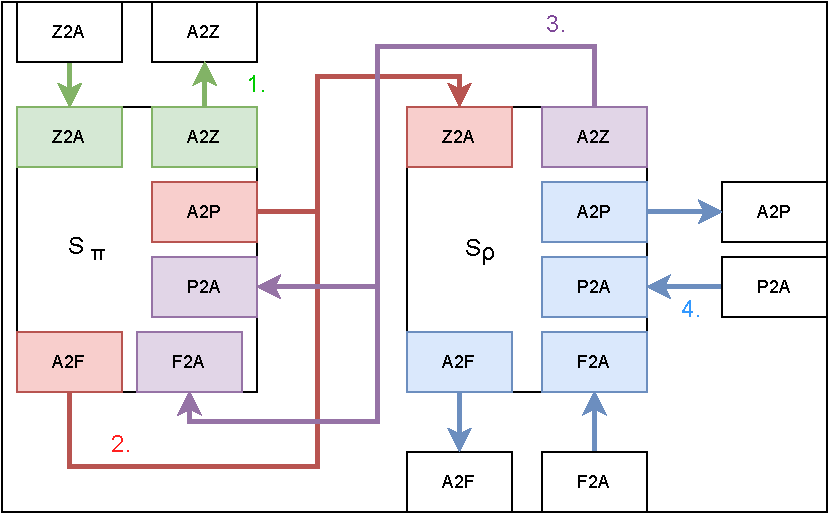
\includegraphics[scale=0.5]{figures/simcomp.pdf}
%\caption{The composed simulators for $\F_1 \xrightarrow{\rho \circ \pi} \F_3$. The real world consists of $(\rho \circ \pi, \F_1)$. Inputs from \Z are for $\F_1$ and dummy parties interacting with $\F_1$, which \SIM{\pi} is equipped to handle. Outputs from \SIM{\pi} are for $\F_2$ and dummy parties of $\F_2$ which \SIM{\rho} is equipped to handle. Finally, outputs from \SIM{\rho} are for $\F_3$ and dummy parties of $\F_3$, which is just the ideal world in Theorem~\ref{thm:composition}.}
%\label{fig:simcomp}
%\end{figure}


\section{Zk} \label{app:zk}
In this section we outline the graph hamiltonicity. Recall $\F_\msf{zk}$ from Section~\ref{sec:commitment}.
$\F_\msf{zk}$ relies on some arbitrary NP relation that can be checked given an instance of a problem and a witness.  

In this section we highlight a zero knowledge protocol that can be built on top of a cryptographic commitment.
The commitment used for this example is more involved than the \Fcom presented in the main body of the paper.
The primary difference is that this \Fcom also possesses an arbitrary message-passing functionality.
It is an important feature as protocols relying on commitment often need a communication channel as well.

We modify the commitment protocol and the simulator for commitment to accomodate this additional functionality. 

\subsection{Commitment With Message Passing}
The types of the channels for this version of \Fcom are summarized before. The type and ordering for the committer and receiver are the same,
but additional labels, for each type, are added to send and receive arbitrary messages. 
\begin{tabbing}
    $\mi{type} \; \m{sender}[a]\{n\} = \ichoice{$\=$ \textcolor{red}{\paypot^2} \mb{Commit}: \m{Int} \product \m{scommitted}[a]\{n\},$ \\
    \>$\textcolor{red}{\paypot^1} \mb{Sendmsg}: \m{a} \product \m{sender}[a]\{n\}}$ \\
    $\mi{senderf2p}[a]\{n\} = \echoice{ \textcolor{red}{\getpot^1} \mb{Recvmsg}: \m{a} \arrow \m{senderf2p}}$
\end{tabbing}
The $\m{Sendmsg}$ label exist along side the other label $\mb{Open}$ as well.
Similarly, the receiver session type from the functionality is edited to add a recvmsg.
\begin{tabbing}
    $\mi{type} \; \m{receiver}[a]\{n\} = \echoice{$\=$\textcolor{red}{\getpot^0} \mb{Commit}: \m{rcommitted}[a]\{n\},$ \\
    \>$\textcolor{red}{\getpot^1} \mb{Recvmsg}: \m{a} \arrow \m{receiver}[a]\{n\}}$ \\
    $\mi{type} \; \m{receiverp2f}[a]\{n\} = \ichoice{\textcolor{red}{\paypot^1} \mb{Sendmsg}: \m{a} \product \m{receiverp2f}[a]\{n\}}$
\end{tabbing}
Finally, the adversary has a special message to get leaked messages from \Fcom:
\begin{tabbing}
    $\mi{type} \; \m{adv}[a] = \ichoice{ \mb{getLeak}: \echoice{$\=$\mb{yes}: \m{a} \arrow \m{adv}[a],$ \\
    \>$\mb{no}: \m{adv}[a]}}$
\end{tabbing}

The protocol $\pi_\msf{com}$ changes in subtle ways. Primarly, the messages they exchange over the channel functionality
is of type 
\begin{lstlisting}[basicstyle=\footnotesize\BeraMonottFamily, frame=single, mathescape]
$\Type$ commsg[a] = Commit | Open Int Int | Msg a 
\end{lstlisting}
This way there is differentiation of messages for both $\Sim_\msf{com}$ and $\pi_\msf{com}$ to know when to output received messages.
Because of this simple change, $\Sim_\msf{com}$ for the corrupt sender, from the main body of the paper, changes only slightly
to accept messages from the enviroment asking for new message leaks from the ideal functionality:
\begin{lstlisting}[basicstyle=\footnotesize\BeraMonottFamily, frame=single, mathescape]
Z2A2F,*,* =>
  $\nget$ {2} K $\$$z_to_a ;
  let m = $\nrecv$ $\$$z_to_a ;
  $\ncase$ m (
    GetLeak =>
      $\$$a_to_f.A2F ;
      $\nsend$ $\$$a_to_f GetLeak ;
      $\ncase$ $\$$a_to_f (
        yes => m = $\nrecv$ $\$$a_to_f ;
               $\$$a_to_z.F2AZ ; $\nsend$ $\$$a_to_z m ;
        no => ()
      )
      $\$$ch <- sim_com_sender[K][K1] <- (* args *) 
    $\tg{(* rest of the cases *)}$
\end{lstlisting}

\subsection{ZK Hamiltonian Cycle}
A zero-knowledge proof of the Hamiltonian Cycle relation is the canonical example of a zk-proof
that can be constructed in UC out of \Fcom~\cite{uccommitments}.

The protocol $\pi_\msf{hampath}$ and the functionality \Fzk rely on a relation checker for a graph
and a possible hamiltonian path. We give the type definition of the process that checks this relation:
\begin{lstlisting}[basicstyle=\footnotesize\BeraMonottFamily, frame=single, mathescape]
$\yo{type}$ Vertex = Int ;
$\yo{type}$ Edge = (Vertex, Vertex) ;
$\yo{type}$ Graph = (Vertex, [Edge]) ; 

$\yo{type}$ zk_relation[a][b] = &{ pair: a $\rightarrow$ b $\rightarrow$ 
  +{ yes: 1, no: 1}}

$\nproc$ ham_relation : . 
  $\vdash$ ($\$$R: zk_relation[Graph][[Edge]]) =
{
  $\ncase$ $\$$R(
    pair =>
      (* v = check the ham cycle *)
      $\nif$ v $\nthen$
        $\$$R.yes ;
      $\nelse$
        $\$$R.no ;
      $\nend$
  )
}
\end{lstlisting}

The hamiltonian path zero knowledge proof protocol uses the multisession extension of \Fcom, $!\Fcom$,
for in order to perform multiple commitments. Notice the type for a party communicating with $!\Fcom$ in 
the type definition of $\pi_\msf{hampath}$ below.
Recall that when wrapped in the multisession wrapper type, the messages from the $\pi_\msf{hampath}$ to $!\Fcom$
passes functional types without ordering even though within \Fcom the session type is being used.
The types that the typedef of $\pi_\msf{hampath}$ are the following (notice they are functional type equivalents of the session types we're seen already):
\begin{lstlisting}[basicstyle=\footnotesize\BeraMonottFamily, frame=single, mathescape]
type comp2f[a] = Commit of Bit | Open | Send of a ;
type comf2p[a] = Commit | Open of Bit | Recv of a ;
type coma2f[a] = GetLeak ;
type comf2a[a] = Yes of a | No ;
\end{lstlisting}

\begin{figure*}
\centering
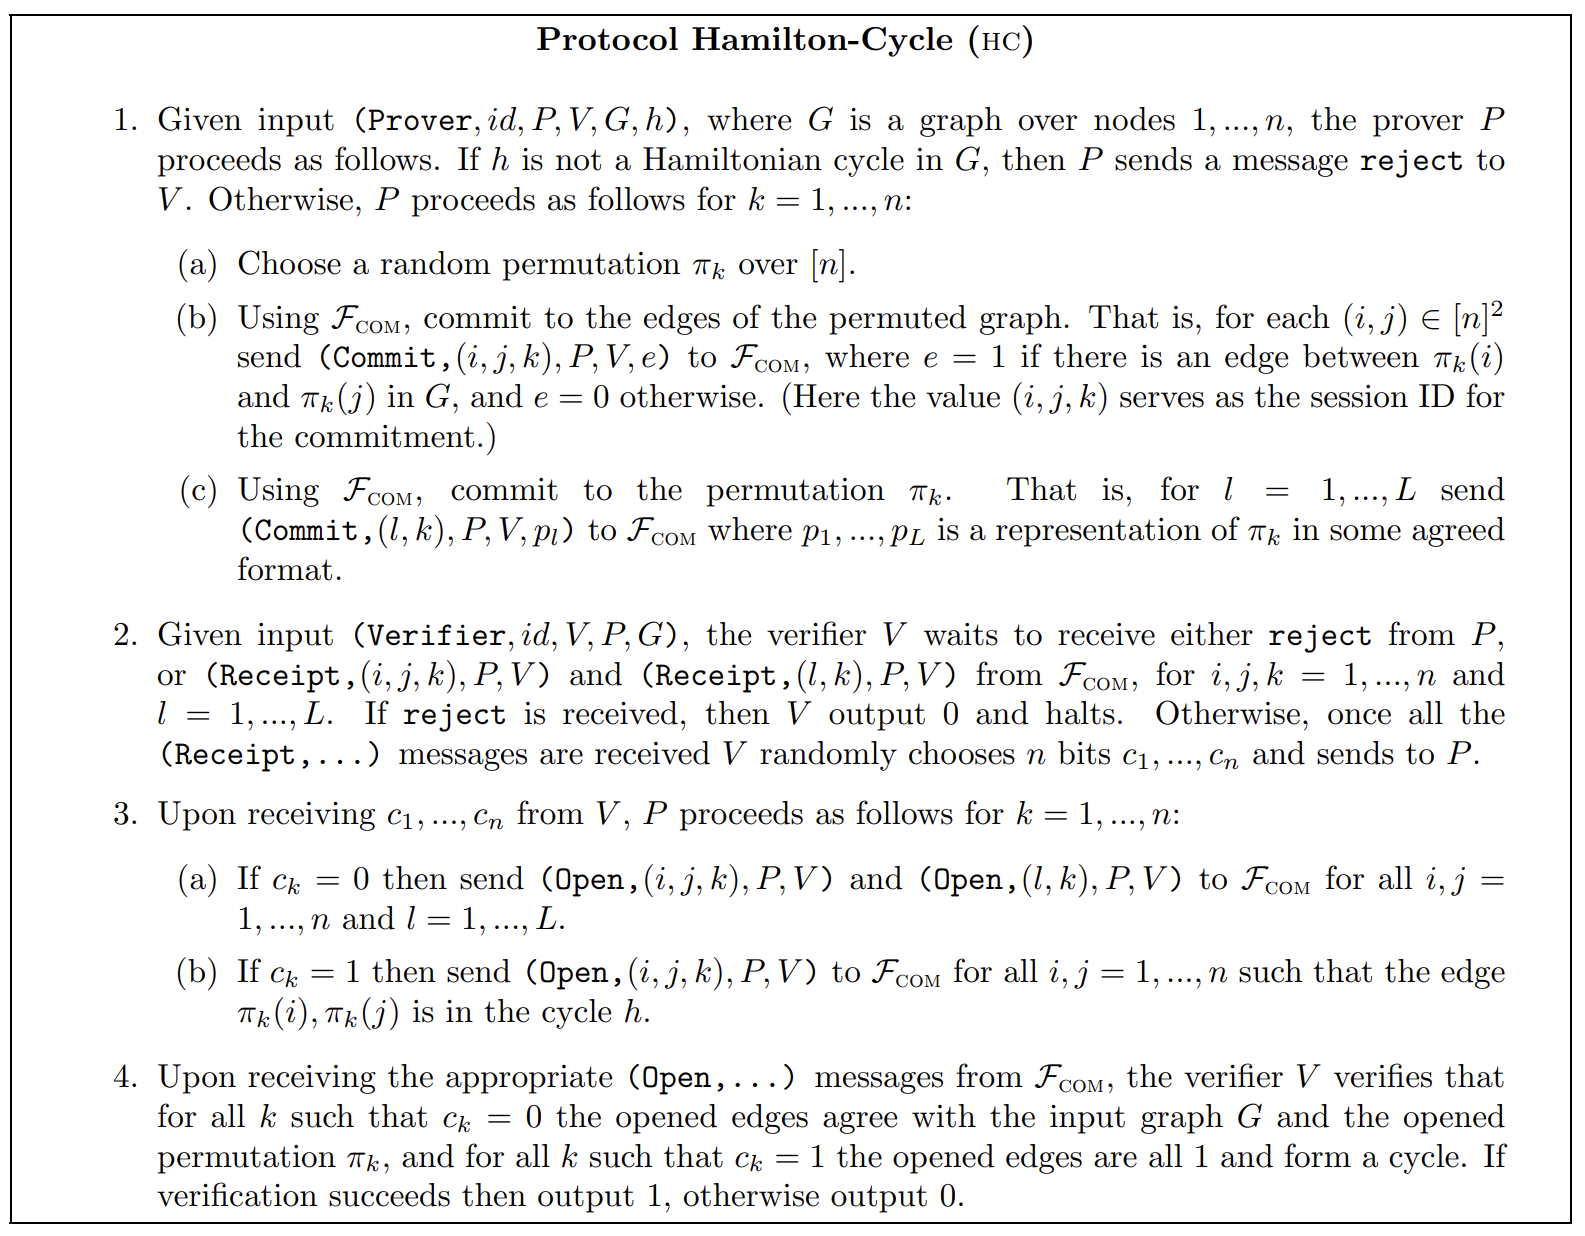
\includegraphics[scale=0.25]{figures/hampathprot.png}
\caption{The UC protocol for a zk-Hamiltonian Cycle protocol in the \Fcom-hybrid world.}
\label{fig:hampathzk}
\end{figure*}

Roughly, the protocol proceeds as follows, and is detailed in Figure~\ref{fig:hampathzk}.
If the hamiltonian cycle given by \Z to the prover passes \inline{ham_relation} it create $k \in \{1..n\}$ different
permutation $\pi_k$ of the nodes and for each one, it creates a commitment for every pair of nodes $i,j$ and creates $n^3$ commitments
where the \m{ssid} is $(i,j,k)$ as detailed by $\inline{ham_sid}$ below. The bit being committed to
is the whether $\pi_k(i)$ and $\pi_k(j)$ have an edge in the original graph. 
Finally the prover commits to each of the $k$ permutations of the graph.  
The verifier selects a series of the $n$ bits which determines, out of the $k$ permutations whether
the open the commitment to the the whole permutation or or open the commitment to the edges that form a cycle
in the permutation. 
The verifier performs the checks described in Figure~\ref{fig:hampathzk}


We detail how the prover code. First we highlight the type for the prover and the verifier.
\begin{tabbing}
    $\mi{type} \; \m{prover}[a]\{n\} = \ichoice{$\=$ \textcolor{red}{\paypot^n} \mb{Commitment}: a \product$ \\ 
    \>$\echoice{ \mb{Yes}: 1, \mb{No}: 1 }}$ \\
    $\mi{type} \; \m{verifier}[a,b]\{n\} = \ichoice{ \textcolor{red}{\paypot^n} \mb{witness}: a \product b \product \m{activate}[a,b]\{n\}}$ \\
    $\mi{type} \; \m{activate}\{n\} = \ichoice{ \textcolor{red}{\paypot^n} \mb{domore}: \m{activate}\{n\}}$
\end{tabbing}

The pro
The prover code for hamiltonian path that sends commitments to $!\Fcom$:
\begin{lstlisting}[basicstyle=\footnotesize\BeraMonottFamily, frame=single, mathescape]
type ham_sid = (Int, Int, Int)

$\nproc$ prot_ham_prover :
  (k: Int), (rng: [Bit]), (sid: session[1]),
  ($\$$z2p: prover[Graph][[Edge]]), ($\$$p2z: 1), 
  ($\$$p2f: p2ms[ham_sid][comp2f]{2}), ($\$$f2p: p2ms[ham_sid][comf2p]{0}) |- ($\$$ch: 1) =
{
  $\ncase$ $\$$z2p (
    witness =>
      $\nget$ \{3\} K $\$$z2p ;
      graph = $\nrecv$ $\$$z2p ; hpath = $\nrecv$ $\$$z2p ;
      $\$$R <- ham_relation <- ;
      $\$$R.pair ; $\nsend$ $\$$R (graph, hpath) ;
      $\ncase$ $\$$R (
        yes => 
          let n = size graph ;
          $\nfor$ k in [1..n] $\nthen$
            $\$$p <- graph_permute ;
            $\$$p.permute ; $\nsend$ $\$$p graph ;
            $\ncase$ $\$$p ( permutation =>
              let newnodes = recv $\$$p ;
              $\nfor$ i in [1..n] $\nthen$
                $\nfor$ j in [1..n] $\nthen$
                  let ssid = (i, j, k)
                  let pi = geti newnodes i
                  let pj = geti newnodes j
                  let e = isedge graph pi pj 
                  $\$$p2ms.p2bf ; $\npay$ \{2\} ;
                  $\nsend$ $\$$p2ms ssid ;
                  $\nsend$ $\$$p2ms (Commit e) ;
                  $\nif$ (j<n) $\nthen$
                    $\ncase$ $\$$z2p ( domore => 
                      $\nget$ {3} K $\$$z2p; )
                  $\nelse$ ()
                $\nend$
                $\nif$ (i<n) $\nthen$
                  $\ncase$ $\$$z2p ( domore => 
                    $\nget$ {3} K $\$$z2p; )
                $\nelse$ ()
              $\nend$
            )
          $\nif$ (k<n) $\nthen$
            $\ncase$ $\$$z2p ( domore => $\nget$ {3} K $\$$z2p; )
          $\nelse$ ()
        no => 
          $\tg{* reject input *)}$
      )
  )
}
\end{lstlisting}

The type of the simulator is straightforward and makes sense given the type of the protocol above. It
relies on some generic template types we haven't seen yet:

\begin{lstlisting}[basicstyle=\footnotesize\BeraMonottFamily, frame=single, mathescape]
$\nproc$ sim_ham_prover[K][K1] :
  (k: Int), (rng: [Bit]), (sid: session[1]),
  ($\$$z_to_a: z2a[K][p2ms[comp2f]][a2ms[coma2f]]{3}), 
  ($\$$a_to_z: a2z[K][ms2p[comf2p]][ms2a[coma2f]]{0}),
  ($\$$p_to_a: p2a[K][zkp2f]{3}), ($\$$a_to_p: a2p[K][zkp2f]{3}), 
  ($\$$a_to_f: zka2f{1}), ($\$$f_to_a: zkf2a{0}),
  ($\$commitment: [Edge]) |- ($\$$c: 1)
\end{lstlisting}

The type of this simulator indicates that it accepts messages from \Z for corrupt protocol parties
according to the real world ideal functionality $!\Fcom$. Therefore, messages are wrapped in the 
\inline{p2ms} type mentioned. 

When composing two protocols, we are already guarantees that the types of protocol being swapped in for the functionality is identical. 
This include the import exchanged as well. 
Recall that composition operator in Section~\ref{sec:execuc}. Applying the operator to the protocol above with $\pi_\msf{com}$ is quite straightforward as the tokens exchanged are the same.
Similarly, composing simulators is trivial as we simply take output for the protocol parties and $\Fcom$ from $\Sim_\msf{com}$ and casts it as \inline{z2p} input for $\Sim_\msf{hampath}$ using an operator as generic as the composition operator itself.


\section{ITM Completeness} \label{app:itm}
%Want to show that NomosUC can capture any ITM configuration and does not capture non-ITM behvior. 
%This corresponds to a compiler in both direction: ITM confiuration $C \Leftrightarrow$ NomosUC configuration $C'$
%
%\paragraph{ITM $\Rightarrow$ NomosUC}.
%The main departure of NomosUC from ITMs is that ITMs work on tapes that are externally writeable whereas processes in NomosUC are connected via channels.
%In the UC literature, a configuration of ITMs is accompanied by a control function that determines which other ITMs a machine can write to.
%NomosUC makes this mechanism explicit by creating channels for two processes to communicated over. 
%At a high level, at any given point an ITM can either wait to received something on its input tape, perform some computation, or write to an externally writeable tape of another ITM.
%A configuration $C$ of ITMs has an equivalent NomosUC configuration $\D \overset{T}{\underset{W}{\vDash}} C' :: \D'$ where channels $\msf{ch} \in \D$ correspond to the communication set of ITM configuration $C$.
%The NomosUC typing rules account for all possible steps an ITM can take: writing with the external/internal choice rules, spawning a new ITM with new channels and composing with the current configuration, etc. \todo{ make more precise but at a high level this argument is pretty clear to see }.

We want to show a bisimulation between NomosUC terms and ITMs.
An ITM $M$ is defined by a unique identity \ID{M} and its code $\mu_M$. 
A system of ITMs is defined by a single initial ITM $I$ with some \ID{I} and a control function \cf.
The control function is applied to every message an ITM sends and defines which ITMs are able to communincate with each other.
In UC, for example, \cf enforces rules such as prohibiting ITMs of different sessions from communicating and stopping \Z from writing input to a corrupt protocol party. 
The control function also serves the imporant purpose that it spwans ITMs when a message is sent to a receiver that doesn't exist yet. It only spawns a machine $M' = (\ID{M'}, \mu_{M'})$ if the message sent to it by some $M$ is \emph{allowed}.

NomosUC differs from this approach to communication in two crucial ways:
\begin{itemize}
	% \item Unlke the single entity that is the ITM, representations of ITMs in NomosUC may span several processes that \emph{become} each other (we define one process \emph{becoming} another later on). We group such processes into a term that represents one ``ITM''. 
	\item NomosUC represents ITMs through multiple processes that act as one. The type system esuresthese processes share import, potential, and work done. For the remainder of this section we will refer to a process or term to be all of the processes that make up one ITM. 
	\item In NomosUC identity mechanism and control function are replaced by channels that directly connect parties that are allowed to communicate. Channels distinguish processes and make an identity mechanism useless. 
		In some cases where shared channels are used, a process might expect multiple others to write to it. In this case, we can assume that protocols implement a mechanism to identify themselves.
	\item In UC, \cf spawns new ITMs went messages are sent to a non-existent ID. A process $P$ spawning $Q$ first creates its channels, then spawns $Q$, and then may send it a message.
\end{itemize}

We show how to convert from an ITM system to a NomosUC configuration, and how to conver a NomosUC term into an ITM. 
In general, the control function can be arbitrary but here we discuss ITM systems specifically with the UC control function.

% %
\subsection{NomosUC $C' \Rightarrow$ ITMs $M'$}
%In NomosUC a process can \emph{step} into a another process and become it. The new process can have different paraeters of different types but retains the same import, potential, state and work done as the previous process. In this sense, it \emph{becomes} another process. 
%For example, an ideal functionality may be captured by three processes $P_1$, $P_2$, and $P_3$ where $P_1$ reads and message from either channels $c_1$ and $c_2$ and steps into $P_2$. 
%$P_2$ may read only from $c_2$ and then step to $P_3$. 
%Finally, $P_3$ waits for another messages from $c_2$ and steps back to $P_1$. 

%Compiling a term or configuration of terms in NomosUC requires two parts: defining a control function, ITM identities, and determing how actions in NomosUC translate to ITM actions.
%ITMs communicate by sending messages that contain the unique identity of the receiver, the code of the receiving ITM, and some amount of import.
%A control function \cf is applied to each message and determines whether the message is \emph{allowed}.
%If a message is \emph{allowed}, \cf delivers the message. If the receiver doesn't exist yet, \cf spawns it with the given identity and code and then delivers the message.
%NomosUC terms carry no name or identifier. We describe below how ITMs are assigned random $k$-bit strings as identities. 
We begin with an initial NomosUC term $e$ and create the initial ITM $M_e$ with a \sid and \pid that are both $k$-bit strings. As no other processes exist, $e$ does not hold any channels to any other processes and must spawn new processes itself.
In UC, this initial ITM is \Z whose code determines the session ID for the rest of the ITMs in the execution.
Notation: from now we call $M_P$ the ITM form of process $P$ (or $P_P$). 

\begin{itemize}
%	\item {\bf Computation Steps.} 
%		Computation is handled differently in NomosUC and ITMs. For example, one computation step in NomosUC may translate to several computation steps in ITMs. Therefore, for the purposes of bisimulation it is important to note that a sufficient bounding polynomial for the resulting ITMs can always be determined that ensures that write operations both fail and succeed in the ITM system if and only if they do in NomosUC.
	\item {\bf Invoking a New Process.} 
		%Terms in NomosUC are frequently run inside of a shell process $shell(\cdot)$ that connects to other shells via communicators but presents a session-typed interface to the process within.~\footnote{This is done for several reasons as explained previously and shown in Figure~\ref{fig:newpandq} as a part of ``providerless channels''}
		All processes in NomosUC derive from some process with an \sid and \pid, and, in the way of UC, when process $P$ spawns process $Q$ we consider the $Q$ to be a subsidiary of $P$.
		Subsidiary processes may not have any explicit ID passed to them in NomosUC so for such processes we follow the UC convention.
		$M_P = (\ID{M_P} = (\sid_P, \pid_P, \mu_{M_P})$ spawns $M_Q$ with the $\ID{M_Q} = (\sid_P, k \xleftarrow{\$} \{0,1\}^k)$.
		Notice that $P$ doesn't need to be the process that spawns $Q$, it just needs to be the first to send it a message.
		%Terms in NomosUC are run in a shell process $shell(\cdot)$ that connects to other shells with communicators, and the shell internally spawns dummy processes that offer linearly typed channels to the actual process. 
		%We dub thiis configuration a ``providerless channel''. 
		%When a term $P$ spawns a new process $Q$ it first creates the communicators that $shell(Q)$ will use and passes their offered channels, the set $\D_Q$, as parameters to $shell(Q)$. 
		%ITM $M_P$ generates a random $k$-bit string as \ID{M_Q} and creates an external write message to ITM $(\ID{M_Q}, \mu_Q)$ with an empty message (recall when processes are spawned in NomosUC no message is sent to them).  \todo{i think you need to give import to spawn the machine, but maybe not because the control function does not use import}
		%When $Q$ is spawned, $P$ holds the endpoints for all of $Q$'s channels so we update \cf to allow communication between \ID{M_P} and \ID{M_Q}.
	\item {\bf Giving a New Process an Existing Channel.} 
		When a process $P$ spawns a process $X$ and gives it a linear channel (with $Q$) endpoint as a paremeter, $P$ relinquishes the endpoint and can no longer communicate on it. 
		%When a shared channel is passed to $X$ both $P$ and $X$ can send/receive on the channel.
		The change from $P$ to $X$ is hidden from $Q$, but in the ITM system without channels we need to define a zero-input message, \msf{commUpdate}, that updates the code of $M_Q$. 
		$M_P$ sends \msf{commUpdate(\ID{M_P}, \ID{M_X})} to $M_Q$ which replaces all message reads/writes to/from $M_P$ with $\ID{M_X}$ if $P$.
	\item {\bf Sending a Message.} 
		Sending messages requires no special treatment when translating from NomosUC to ITMs. The identities of the recipients are known to the sending ITMs, and the NomosUC construction ensures that sending channels to other processes never results in a violation of the UC control function.
		In UC it is important to specify what tape a message is being written on but the UC \cf enforces such rules.
	\item {\bf Reading a Message.} 
		NomosUC terms are explicit about which channels they read on, and, in general attempt to read on all channels at once. This corresponds nicely to the ITM setting where an ITM $M_P$ can mimic the behavior of $P$ by only accepting messages from ITMS $M_X$ where $X$ is connected to $P$ by a channel. 
\end{itemize}

% %
\subsection{ITMs $M' \Rightarrow$ NomosUC $C'$}
We first point out that coverting ITMs to NomosUC terms requires defining the types for communication between different pairs of ITMs.
In fact, for an ITM $M_P$ all possible message types that $P$ may communicate with must be defined at compiled time. 

\paragraph{Naming and Defining Types.}
We provide a minimal structure for the types defined for the resulting NomosUC terms.
Namely, we can simplify the construction by capturing all communication using communiators and the shared channels that they offer. 
Recall that with providerless channels we only care about interaction between the shell processes. 
%For the purposes of this argument this greatly simplified the construction~\footnote{Providerless channels are an abstraction created specifically to capture the UC framework in a way that session types are meaningful and useful to the programmer.}
Along with communicators, we make use of the existing addressin scheme in the ITM model, and ensure all messages sent by some $P$ carries \ID{M_P} alogside it.

%For example, say an ITM $M_1$ may communicate with $M_2$ and $M_3$, and the reslting types between $P_1$ \& $P_2$ and $P_1$ \& $P_3$ are different.
%Then the resulting $P_1$ is parameterized by at least two shared channes of type $\msf{comm}[(ID, a)]$ and $\msf{comm}[(ID, b)]$ where \inline{type ID = Int}, a $k$-bit number.
We start with a system with the initial ITM $I$ and the UC control function \cf.
The NomosUC process for $I$ has no channels as input parameters as no other processes exist yet.
\cf is easily captures by NomosUC as \msf{execUC} spawns all the main parties of the execution and the type system prevents sending channels to other ITMs over channels and enabling communication between, say, the environment and a corrupt party.

\begin{itemize}
	\item {\bf Invoking a New ITM.} 
		When a process $P_M$ spawns a new $P_N$ it first creates the channels $P_N$ communicates over. 
		For each message type $t$ that $P_N$ may communicate through, $P_M$ spawns a communicator parameterizes with $t$.
		At a bare minimum at least one channel is required per message type that $P_N$ accepts as defined by \cf. 
		This ensures a generic way to handle an arbitrary number of connections (for each message type) where messages include the $\ID{sender}$.
		Much like an ITM, $P_N$ attempts to read from all of its channels and uses \ID{sender} to perform some computation.
		%When spawned, $P_N$ then reads the message sent by $P_M$ (corresponds to the message $M_M$ sends $M_N$ causing the ITM to be spawned).
	\item {\bf Sending a message.} 
		All messages from some $P_m$ in the resulting configuration are sent with \ID{M_m} because we rely on shared channels to realize the ITM system (as opposed to one channel per ITM/term). 
		A key departure from the ITM model is that the static nature of types requires that the same amount of import be sent with every message, however sending more import than necessary doesn't pose any trouble. We discussed, briefly, how to handle import in NomosUC in a previous section.   
		%This requirement can be overcome by defining the type for communication between some $P$ and $Q$ to be the maximum ever sent between $M_P$ and $M_Q$. 
		% Propoagating this approach to defining import requirements to all types in the system, we ensure we arrive at a satisfying assignment of import. 
	\item {\bf Reading a message.} 
		Reading messages is more explicit in NomosUC than in ITMs. 
		In NomosUC individual processes must be explicit with  what channels to read on. 
		For the sake of simplicity every resulting process waits to read on all channels (unless their type sugests otherwise) and executes the ITM code in response to messages.
\end{itemize}



%The challenge here is that the channels of a NomosUC process are are defined at the time that the process is invoked. This fixes the set of machines that $P$ can communicate with static.
%$P$ can spawn its own processes and communicate with more processes that way. 
%This poses a problem because an arbitrary ITM system may randomly decide any comunication structure that NomosUC may not be able to capture. 
%The real question comes down to: can NomosUC capture every control function? I think with provider-less channels that is possible.
%
%An example that shows this off is the following:
%\begin{itemize}
%	\item An initial ITM $M_1$ spawns ITMs $M_2, M_3, M_4$. $M_3$ flips a coin and spawns either only $M_31$ or both 
%	\item The control function states that $M_1$ can communicate with all other ITMs and that $M_2$ and $M_3$ an communicate and $M_4$ can communicate with $M_31$ and $M_32$.
%\end{itemize}
%
%NomosUC version
%\begin{itemize}
%	\item Initial process $P_1$. 
%	\item $P_1$ creates the communicators for the providerless channels of $P_2, P_3$ and $P_4$. \todo{ What is the type of the linear channels that the processes see?}.
%	\item $P_2$ and $P_3$ are given the communicator channel for their connection. $P_3$ is given the communicator channel connecting for $P_4$.
%	\item $P_3$ flips a coin and spawns one of $P_31$ or $P_32$ and gives it the channel for the communicator with $P_4$.
%\end{itemize}
%In this setting because the communicator channel is a shared resource each of the processes that has ever obtained it can acquire the channel and communicate using it. 
%In the above example it means that $M_1$, $M_3$ and $M_4$ can all communicate with $M_31$, $M_32$. If the control function prohibits such communication we must rely on the code the process to not communicate
%over the channels. 
%The providerless channels are virtually running the process and giving it linear channels for its communication. The type of the communicator between $P_31$/$P_32$ and $P_4$ means that it remains abstract in $P_3$ and is concretized in $P_31$/$P_32$.
%
%Proving this direction is straihtforward. The proof proceeds by describing how to compile an ITM configuration into a NomosUC configuration and ever ITM action into a process action.
%
%\paragraph{Compiling an ITM Configuration to NomosUC}
%As described above an ITM configuration consits of ITMs and a control function which defines the communication set for each ITM.
%The operations available to an ITM are to take a computation step, write something to another ITM's tape, or read some input on on of its tapes. 
%In NomosUC, our external $\with$ and internal $\ichoiceop$ and the typing rules $\oplus R$ and $\oplus L$ capture sending and receiving messages between a pair of ITMs. 
%\todo{ some transition text here }
%
%
%% need to show up to translate and existing configuration from ITM to NomosUC
%% need to show how to translate every possible action that an ITM takes to a NomosUC action --> show how that preserves the same properties of import as in ITMs
%% need to show how to spawn new ITMs/processes 
%Given a configuration $C$ of ITMs:
%\begin{itemize}
%\item For every ITM $M \in F$ with communication set $C_M$: for every $M' \in C_M$ we spawn processes $M$ and all $M'$ and connect them with a providerless channel of type specified by the code of machines $M'$ and the definition of the process code.
%\item The basic computation step in an ITM is different from the fundamental computation step of a NomosUC process. 
%However, by manipulating the bouding polynomial, we can equate multiple computation steps in an ITM to a single step of a process and vice versa.
%Modulo the conversation rate between computation steps in ITMs vs NomosUC processes, the token context validity rules in Section~\ref{sec:basic} ensure that ITMs and their corresponding processes halt after the same number of computationsl steps, i.e. $T(n)$ steps where $n$ is the net import held.
%\item The same reasoning applies to write operations where the token validty rule ensures that for security parameter $k$ write operations succeed only if there is available import \todo{tis sounds so hand wavy and imprecise I hate it}
%\item When an ITM $M \in F$ spawns a new ITM $M'$ such that $M' \in C_M$: the Nomos process creates the providerless channels for ITM $M'$ and stores them to communicate with $M'$ in the future.
%\end{itemize}


%\begin{itemize}
%	\item When a term $P$ spawns a new process $Q$ it creates the channels that $Q$ will use and passes them as parameters to $Q$. ITM $M_P$ creates an external write message with the code for term with a randomly generated $k$-bit string as the ID for new ITM $M_Q$, and the ITM code for process $Q$ (including its initial state). The control function is updated $\forall X$ s.t. $X$ shares and endpoint of a channel of $Q$, we update the control function $C$ to allow $M_Q$, $M_X$ to write to each other.
%	\item When a term $P$ spawns a new process $Q$ and gives it an exisitng channel $c$ connecting $P$ and some $X$, we update $C$ to allow communication between $M_X$ and $M_Q$ and disallow communication between $M_P$ and $M_X$. We require that all ITMs accept special messages informing them of the ITM change. In this example, $M_P$ sends a zero import message to $M_X$ informing it of the identity of $M_Q$ and telling it to replace $ID(M_P)$ with $ID(M_Q)$ for the remainder of its code. $M_X$ accepts the message and activates $M_P$ again that then spawns $M_X$.
%	\item \todo{actually when spawning a channel with no other endpoint, the spawning process is the endpoint so we can set control function to do that then use the above defined message when the endpoint is actually given to someone else.}
%\end{itemize}
%The fundamental unit of computation in ITMs and Nomos process is different so by manipulation of the bounding polynomial our type system ensures that messages sent with import succeed if and only if they do so in the corresponding ITM system.
%
%\paragraph{Compiling NomosUC Terms into ITMs.}
%Like ITMs, terms in NomosUC can do one of three things: execute a computation step, wait to read a message, and send a message.
%We describe how these operations in NomosUC are captured by ITMs.
%\begin{itemize}
%	\item {\bf Computation Steps.} The fundamental computation unit that NomosUC potential is able to track is not the same as the ITM. Therefore, we need to ensure that operations in an ITM fail or succeed the same way as the corresponding NomosUC process. If the bounding polynomial of a NomosUC term is $T(x)$ then this is trivially achieved by relaxing the corresponding bounding polyomial for ITMs to account for the greater number of computation steps per NomosUC instruction. 
%	\item {\bf Write Operations.} From the previous discussion, the ITM $M_P$ is updated to reflect which processes hold the endpoints of the channels of $P$. On write operations, there is nothing special that needs to be done to accomodate this. By definition, $M_P$ will never attempt to write to an ITM that doesn't exist as the NomosUC channel always has processes at each endpoint. The import is handled similar to the above case.
%	\item {\bf Reading a Message.} NomosUC process an read on any number of channels at a given time. For example a Nomos term may be composed of two processes $P_1$ and $P_2$ where $P_1$ waits on a channels with $Q$ and $Q'$ then step to process $P_2$ that waits only on a channel with $Q$. In such cases, the ITM code is simply modeled to reflect this decision and any ``unexpected'' writes from ITMs that the code is not explicitly expecting messages from are ignored and the receiving ITM never relinquishes activation. Like the NomosUC code, the program is locked and can no longer make any progress. 
%\end{itemize}
%
%\paragraph{Handling Import.}
%We emphasize again that the fundamental unit of computation for ITMs is not the same as that of NomosUC terms. 
%However, this is easily dealt with selecting a larger bounding polynomial for the ITM system than for the NomosUC term. 
%This takes care of differences in amount of computation while ensuring messages can carry/deliver the same import and succeed if and only if they succeed in the ITM system.




%\paragraph{Modelling processes as ITMs.}
%Read operations in NomosUC are blocking and must specify which channels are being read from. In the toy example above, and ITM that captures $P_2$ would only react to messages written to its tape by an ITM for the protocol party and ignore messages from the adversary.
%
%
%
%We provide a compiler from a NomosUC configuration to an ITM system. 
%More specifically, we show how to convert a term $e$ into an ITM. 
%Terms in NomosUC can be made up of multiple process terms and are the logical equivalent of an ITM in NomosUC. 
%
%Take a simple process configuration:
%\begin{itemize}
%	\item Tree processes P1, P2, and P3. 
%	\item Processes P1 becomes process P2 at some point.
%	\item Processes P1 and P2 are connected to P3 through a providerless channels A and B.
%	\item Process p1 waits on both channels A and B with the choice operator.
%	\item P3 flips a coin and chooses to write on one of channels A or B.
%	\item Once P1 reads one of the channels it becomes P2.
%	\item P2 only attemps reads on channel A.
%\end{itemize}
%
%We collected processes like $P_1$, $P_2$ into a single terms as they share the same state, channels, import, potential, and work done.
%Our compilation step converts terms into ITMs rather than individual processes. 
%
%
%\subsection{Control Function}
%The control function in UC enforces communication rules between ITMs and their identities.
%NomosUC has no inherent naming scheme for processes because it directly connects processes with channels. 
%We propose the following nameing scheme and control function. Suppose an initial process $PI$ that is not connected by channels to any other process.
%The initial ITM corresponding to $PI$ is $MI = (ID, \mu)$ where $ID$ is a random $k$-bit string and $\mu$ is its code.
%
%When $PI$ spawns a new processi $P_1$, it creates channels for the process to use and passes them as parameters to $P_1$. 
%Machine $MI$  

%This direction is more complicated than the previous subsection. Here, we must show that NomosUC configurations can be represented as an ITM system and that NomosUC does not allow non-ITM behavior.
%NomosUC must capture the activation rules of ITMs, ensure an ITM never performs more computation than its import provides, and never performs super-polynomial computation. 
%The first of these requirements is satisfied by the write token $\wt$ that ensures no NomosUC programs cannot perform computation and write to other processes without first being written to, i.e. activated.
%We further fall back to our definition of a valid token context which ensures that both regular ITMs and sandboxed ITMs (through $\m{withdrawTokens}$) never perform computation over a fixed polynomial in their \emph{net} import.
%
%So far we have only shown that NomosUC configurations share the same properties as ITM systems. 
%We describe how to compile NomosUC configurations into ITM systems.
%In NomosUC, a process $P1$ with $ID = (SID, pid)$ can step to another process $P2$, with the same $ID$,  that may step to another process eventually stepping back to $P1$. 
%We compile such collections of processes into a single ITM $M$ with the communication set $C$, where $C$ is the the set of $ID$s of all processes the collection of processes has a channel to. 
%For example, a process $P_1 :: A$ becomes $P_2 :: B$ in the future, $P_2$ becomes $P_3 :: C$ at some point, $P_3$ becomes $P_2$, and the cycle repeats. 
%If $P_3$ shares channels to processes with IDs $x$, $y$, and $z$, we set the commnucation set of the corresponding ITM to $\{ x, y, z \}$.

%Given a NomosUC configuration $\D_0 \overset{T}{\underset{W}{\vDash}} \config :: \D_1$:
%\begin{itemize}
%\item For every process $(\Sg \semi k \semi \Tokens \semi \Psi \semi D \entailpot{q}{q'} P :: x) \in \config$ we create an ITM $M$ with communication set specified by the endpoint for every $c \in D$ 
%\end{itemize}
%
%% nomosuc can capture non-ITM behavior but if we assume we start with some valid ITM configuration then we're good
%% need to translate every step that the NomosUC configuration can take to an ITM step
%% show that none of the possible processes actions in NomosUC lead to a configuration without an ITM analog
%% for the above need explicit compiler from NomosUC to ITMs and need to determine when compilation is not possible
%% potentially, the above means that we need to first define what constitutes non-ITM behavior: import computations fail / non-polynomial, write before read / activation rules
%\begin{itemize}
%\item Spawning ITMs: \todo{ there's a key difference herer in that with regular ITM systems when a new ITM is spawned it is initialized with a communication set that can include machines that aren't the spawning machine. But in NomosUC we have that the spawning rocess creates the chanels and stores them but can not send the send them over a channel to another ITM. It can only spawn other new processes which can communicate with other spawned machines. }
%\item internl/external choice (write operation)
%\item taking a single computation step (refine above bullet point)
%\item simulating other ITMs through withdrawTokens and sandboxing
%\end{itemize}





\pagebreak

\end{document}
